% **************************************************************************************************************
% A Classic Thesis Style
% An Homage to The Elements of Typographic Style
%
% Copyright (C) 2015 André Miede http://www.miede.de
%
% If you like the style then I would appreciate a postcard. My address 
% can be found in the file ClassicThesis.pdf. A collection of the 
% postcards I received so far is available online at 
% http://postcards.miede.de
%
% License:
% This program is free software; you can redistribute it and/or modify
% it under the terms of the GNU General Public License as published by
% the Free Software Foundation; either version 2 of the License, or
% (at your option) any later version.
%
% This program is distributed in the hope that it will be useful,
% but WITHOUT ANY WARRANTY; without even the implied warranty of
% MERCHANTABILITY or FITNESS FOR A PARTICULAR PURPOSE.  See the
% GNU General Public License for more details.
%
% You should have received a copy of the GNU General Public License
% along with this program; see the file COPYING.  If not, write to
% the Free Software Foundation, Inc., 59 Temple Place - Suite 330,
% Boston, MA 02111-1307, USA.
%
% **************************************************************************************************************
\RequirePackage{fix-cm} % fix some latex issues see: http://texdoc.net/texmf-dist/doc/latex/base/fixltx2e.pdf
\documentclass[ twoside,openright,titlepage,numbers=noenddot,headinclude,%1headlines,% letterpaper a4paper
                footinclude=true,cleardoublepage=empty,abstractoff, % <--- obsolete, remove (todo)
                BCOR=5mm,paper=a4,fontsize=11pt,%11pt,a4paper,%
                francais,ngerman,american,%
                ]{scrreprt}

%********************************************************************
% Note: Make all your adjustments in here
%*******************************************************
% ****************************************************************************************************
% classicthesis-config.tex 
% formerly known as loadpackages.sty, classicthesis-ldpkg.sty, and classicthesis-preamble.sty 
% Use it at the beginning of your ClassicThesis.tex, or as a LaTeX Preamble 
% in your ClassicThesis.{tex,lyx} with % ****************************************************************************************************
% classicthesis-config.tex 
% formerly known as loadpackages.sty, classicthesis-ldpkg.sty, and classicthesis-preamble.sty 
% Use it at the beginning of your ClassicThesis.tex, or as a LaTeX Preamble 
% in your ClassicThesis.{tex,lyx} with % ****************************************************************************************************
% classicthesis-config.tex 
% formerly known as loadpackages.sty, classicthesis-ldpkg.sty, and classicthesis-preamble.sty 
% Use it at the beginning of your ClassicThesis.tex, or as a LaTeX Preamble 
% in your ClassicThesis.{tex,lyx} with \input{classicthesis-config}
% ****************************************************************************************************  
% If you like the classicthesis, then I would appreciate a postcard. 
% My address can be found in the file ClassicThesis.pdf. A collection 
% of the postcards I received so far is available online at 
% http://postcards.miede.de
% ****************************************************************************************************


% ****************************************************************************************************
% 0. Set the encoding of your files. UTF-8 is the only sensible encoding nowadays. If you can't read
% äöüßáéçèê∂åëæƒÏ€ then change the encoding setting in your editor, not the line below. If your editor
% does not support utf8 use another editor!
% ****************************************************************************************************
\PassOptionsToPackage{utf8}{inputenc}
	\usepackage{inputenc}

% ****************************************************************************************************
% 1. Configure classicthesis for your needs here, e.g., remove "drafting" below 
% in order to deactivate the time-stamp on the pages
% ****************************************************************************************************
\PassOptionsToPackage{eulerchapternumbers,listings,drafting,%
					 pdfspacing,%floatperchapter,%linedheaders,%
					 %subfig,
					 beramono,eulermath,parts}{classicthesis}                                        
% ********************************************************************
% Available options for classicthesis.sty 
% (see ClassicThesis.pdf for more information):
% drafting
% parts nochapters linedheaders
% eulerchapternumbers beramono eulermath pdfspacing minionprospacing
% tocaligned dottedtoc manychapters
% listings floatperchapter subfig
% ********************************************************************


% ****************************************************************************************************
% 2. Personal data and user ad-hoc commands
% ****************************************************************************************************
\newcommand{\myTitle}{Measurement-based inter-domain traffic engineering\xspace}
\newcommand{\mySubtitle}{scalability, data interpretation and network event visibility\xspace}
%\newcommand{\myDegree}{Doktor-Ingenieur (Dr.-Ing.)\xspace}
\newcommand{\myName}{Wenqin Shao\xspace}
\newcommand{\myProf}{Luigi Ianonne\xspace}
%\newcommand{\myOtherProf}{Put name here\xspace}
\newcommand{\mySupervisor}{Jean-Louis Rougier\xspace}
\newcommand{\myFaculty}{INFRES\xspace}

\newcommand{\myDepartment}{Department of Network and Computer Science\xspace}
\newcommand{\myUni}{Télécom ParisTech\xspace}
\newcommand{\myLocation}{Paris\xspace}
\newcommand{\myTime}{August 2017\xspace}
\newcommand{\myVersion}{version 0.3\xspace}

% ********************************************************************
% Setup, finetuning, and useful commands
% ********************************************************************
\newcounter{dummy} % necessary for correct hyperlinks (to index, bib, etc.)
\newlength{\abcd} % for ab..z string length calculation
\providecommand{\mLyX}{L\kern-.1667em\lower.25em\hbox{Y}\kern-.125emX\@}
\newcommand{\ie}{i.\,e.}
\newcommand{\Ie}{I.\,e.}
\newcommand{\eg}{e.\,g.}
\newcommand{\Eg}{E.\,g.} 
% ****************************************************************************************************


% ****************************************************************************************************
% 3. Loading some handy packages
% ****************************************************************************************************
% ******************************************************************** 
% Packages with options that might require adjustments
% ******************************************************************** 
%\PassOptionsToPackage{ngerman,american}{babel}   % change this to your language(s)
% Spanish languages need extra options in order to work with this template
%\PassOptionsToPackage{spanish,es-lcroman}{babel}
	\usepackage{babel}                  

\usepackage{csquotes}
\PassOptionsToPackage{%
    %backend=biber, %instead of bibtex
	backend=bibtex8,bibencoding=ascii,%
	language=auto,%
	style=numeric-comp,%
    %style=authoryear-comp, % Author 1999, 2010
    %bibstyle=authoryear,dashed=false, % dashed: substitute rep. author with ---
    sorting=ynt, % name, year, title
    maxbibnames=10, % default: 3, et al.
    %backref=true,%
    natbib=true % natbib compatibility mode (\citep and \citet still work)
}{biblatex}
    \usepackage{biblatex}

\PassOptionsToPackage{fleqn}{amsmath}       % math environments and more by the AMS 
    \usepackage{amsmath}
    \usepackage{amssymb}

% ******************************************************************** 
% General useful packages
% ******************************************************************** 
\PassOptionsToPackage{T1}{fontenc} % T2A for cyrillics
    \usepackage{fontenc}     
\usepackage{textcomp} % fix warning with missing font shapes
\usepackage{scrhack} % fix warnings when using KOMA with listings package          
\usepackage{xspace} % to get the spacing after macros right  
\usepackage{mparhack} % get marginpar right
\usepackage{fixltx2e} % fixes some LaTeX stuff --> since 2015 in the LaTeX kernel (see below)
%\usepackage[latest]{latexrelease} % will be used once available in more distributions (ISSUE #107)
\PassOptionsToPackage{printonlyused,smaller}{acronym} 
    \usepackage{acronym} % nice macros for handling all acronyms in the thesis
    %\renewcommand{\bflabel}[1]{{#1}\hfill} % fix the list of acronyms --> no longer working
    %\renewcommand*{\acsfont}[1]{\textsc{#1}} 
    %\renewcommand*{\aclabelfont}[1]{\acsfont{#1}}
    %\renewcommand*{\aclabelfont}[1]{\acsfont{#1}}
   	%\def\bflabel#1{{#1\hfill}}
   	\def\bflabel#1{{\acsfont{#1}\hfill}}
  	\def\aclabelfont#1{\acsfont{#1}}
\usepackage{fancyvrb}
\usepackage{algorithmicx, algpseudocode}

\usepackage{mathtools}

\usepackage{amsthm}
\newtheorem*{assumption*}{\assumptionnumber}
\providecommand{\assumptionnumber}{}
\makeatletter
\newenvironment{assumption}[2]
 {%
  \renewcommand{\assumptionnumber}{Assumption #1-\textit{#2}}%
  \begin{assumption*}%
  \protected@edef\@currentlabel{#1-\textit{#2}}%
 }
 {%
  \end{assumption*}
 }
\makeatother

\newtheorem*{heuristic*}{\heuristicnumber}
\providecommand{\heuristicnumber}{}
\makeatletter
\newenvironment{heuristic}[2]
 {%
  \renewcommand{\heuristicnumber}{Heuristic #1-\textit{#2}}%
  \begin{heuristic*}%
  \protected@edef\@currentlabel{#1-\textit{#2}}%
 }
 {%
  \end{heuristic*}
 }
\makeatother


\usepackage{multicol}
\usepackage{multirow}
\usepackage{booktabs}
% ****************************************************************************************************


% ****************************************************************************************************
% 4. Setup floats: tables, (sub)figures, and captions
% ****************************************************************************************************
\usepackage{tabularx} % better tables
    \setlength{\extrarowheight}{3pt} % increase table row height
\newcommand{\tableheadline}[1]{\multicolumn{1}{c}{\spacedlowsmallcaps{#1}}}
\newcommand{\myfloatalign}{\centering} % to be used with each float for alignment
\usepackage{caption}
% Thanks to cgnieder and Claus Lahiri
% http://tex.stackexchange.com/questions/69349/spacedlowsmallcaps-in-caption-label
% [REMOVED DUE TO OTHER PROBLEMS, SEE ISSUE #82]    
%\DeclareCaptionLabelFormat{smallcaps}{\bothIfFirst{#1}{~}\MakeTextLowercase{\textsc{#2}}}
%\captionsetup{font=small,labelformat=smallcaps} % format=hang,
\captionsetup{font=small} % format=hang,
%\usepackage{subfig}
\usepackage{subcaption}

\usepackage{rotating}
\usepackage{pdflscape}

% ****************************************************************************************************


% ****************************************************************************************************
% 5. Setup code listings
% ****************************************************************************************************
\usepackage{listings} 
%\lstset{emph={trueIndex,root},emphstyle=\color{BlueViolet}}%\underbar} % for special keywords
\lstset{language=[LaTeX]Tex,%C++,
    morekeywords={PassOptionsToPackage,selectlanguage},
    keywordstyle=\color{RoyalBlue},%\bfseries,
    basicstyle=\small\ttfamily,
    %identifierstyle=\color{NavyBlue},
    commentstyle=\color{Green}\ttfamily,
    stringstyle=\rmfamily,
    numbers=none,%left,%
    numberstyle=\scriptsize,%\tiny
    stepnumber=5,
    numbersep=8pt,
    showstringspaces=false,
    breaklines=true,
    %frameround=ftff,
    %frame=single,
    belowcaptionskip=.75\baselineskip
    %frame=L
} 
% ****************************************************************************************************             


% ****************************************************************************************************
% 6. PDFLaTeX, hyperreferences and citation backreferences
% ****************************************************************************************************
% ********************************************************************
% Using PDFLaTeX
% ********************************************************************
\PassOptionsToPackage{pdftex,hyperfootnotes=false,pdfpagelabels}{hyperref}
    \usepackage{hyperref}  % backref linktocpage pagebackref
\pdfcompresslevel=9
\pdfadjustspacing=1 
\PassOptionsToPackage{pdftex}{graphicx}
    \usepackage{graphicx} 
 

% ********************************************************************
% Hyperreferences
% ********************************************************************
\hypersetup{%
    %draft, % = no hyperlinking at all (useful in b/w printouts)
    colorlinks=true, linktocpage=true, pdfstartpage=3, pdfstartview=FitV,%
    % uncomment the following line if you want to have black links (e.g., for printing)
    %colorlinks=false, linktocpage=false, pdfstartpage=3, pdfstartview=FitV, pdfborder={0 0 0},%
    breaklinks=true, pdfpagemode=UseNone, pageanchor=true, pdfpagemode=UseOutlines,%
    plainpages=false, bookmarksnumbered, bookmarksopen=true, bookmarksopenlevel=1,%
    hypertexnames=true, pdfhighlight=/O,%nesting=true,%frenchlinks,%
    urlcolor=webbrown, linkcolor=RoyalBlue, citecolor=webgreen, %pagecolor=RoyalBlue,%
    %urlcolor=Black, linkcolor=Black, citecolor=Black, %pagecolor=Black,%
    pdftitle={\myTitle},%
    pdfauthor={\textcopyright\ \myName, \myUni, \myFaculty},%
    pdfsubject={},%
    pdfkeywords={},%
    pdfcreator={pdfLaTeX},%
    pdfproducer={LaTeX with hyperref and classicthesis}%
}   

\usepackage{bookmark}
% ********************************************************************
% Setup autoreferences
% ********************************************************************
% There are some issues regarding autorefnames
% http://www.ureader.de/msg/136221647.aspx
% http://www.tex.ac.uk/cgi-bin/texfaq2html?label=latexwords
% you have to redefine the makros for the 
% language you use, e.g., american, ngerman
% (as chosen when loading babel/AtBeginDocument)
% ********************************************************************
\makeatletter
\@ifpackageloaded{babel}%
    {%
       \addto\extrasamerican{%
			\renewcommand*{\figureautorefname}{Figure}%
			\renewcommand*{\tableautorefname}{Table}%
			\renewcommand*{\partautorefname}{Part}%
			\renewcommand*{\chapterautorefname}{Chapter}%
			\renewcommand*{\sectionautorefname}{Section}%
			\renewcommand*{\subsectionautorefname}{Section}%
			\renewcommand*{\subsubsectionautorefname}{Section}%     
                }%
       \addto\extrasngerman{% 
			\renewcommand*{\paragraphautorefname}{Absatz}%
			\renewcommand*{\subparagraphautorefname}{Unterabsatz}%
			\renewcommand*{\footnoteautorefname}{Fu\"snote}%
			\renewcommand*{\FancyVerbLineautorefname}{Zeile}%
			\renewcommand*{\theoremautorefname}{Theorem}%
			\renewcommand*{\appendixautorefname}{Anhang}%
			\renewcommand*{\equationautorefname}{Gleichung}%        
			\renewcommand*{\itemautorefname}{Punkt}%
                }%  
            % Fix to getting autorefs for subfigures right (thanks to Belinda Vogt for changing the definition)
            \providecommand{\subfigureautorefname}{\figureautorefname}%             
    }{\relax}
\makeatother


% ****************************************************************************************************
% 7. Last calls before the bar closes
% ****************************************************************************************************
% ********************************************************************
% Development Stuff
% ********************************************************************
\listfiles
%\PassOptionsToPackage{l2tabu,orthodox,abort}{nag}
%   \usepackage{nag}
%\PassOptionsToPackage{warning, all}{onlyamsmath}
%   \usepackage{onlyamsmath}

% ********************************************************************
% Last, but not least...
% ********************************************************************
\usepackage{classicthesis} 
% ****************************************************************************************************


% ****************************************************************************************************
% 8. Further adjustments (experimental)
% ****************************************************************************************************
% ********************************************************************
% Changing the text area
% ********************************************************************
%\linespread{1.05} % a bit more for Palatino
%\areaset[current]{312pt}{761pt} % 686 (factor 2.2) + 33 head + 42 head \the\footskip
%\setlength{\marginparwidth}{7em}%
%\setlength{\marginparsep}{2em}%

% ********************************************************************
% Using different fonts
% ********************************************************************
%\usepackage[oldstylenums]{kpfonts} % oldstyle notextcomp
%\usepackage[osf]{libertine}
%\usepackage[light,condensed,math]{iwona}
%\renewcommand{\sfdefault}{iwona}
%\usepackage{lmodern} % <-- no osf support :-(
%\usepackage{cfr-lm} % 
%\usepackage[urw-garamond]{mathdesign} <-- no osf support :-(
%\usepackage[default,osfigures]{opensans} % scale=0.95 
%\usepackage[sfdefault]{FiraSans}
% ****************************************************************************************************

% ****************************************************************************************************  
% If you like the classicthesis, then I would appreciate a postcard. 
% My address can be found in the file ClassicThesis.pdf. A collection 
% of the postcards I received so far is available online at 
% http://postcards.miede.de
% ****************************************************************************************************


% ****************************************************************************************************
% 0. Set the encoding of your files. UTF-8 is the only sensible encoding nowadays. If you can't read
% äöüßáéçèê∂åëæƒÏ€ then change the encoding setting in your editor, not the line below. If your editor
% does not support utf8 use another editor!
% ****************************************************************************************************
\PassOptionsToPackage{utf8}{inputenc}
	\usepackage{inputenc}

% ****************************************************************************************************
% 1. Configure classicthesis for your needs here, e.g., remove "drafting" below 
% in order to deactivate the time-stamp on the pages
% ****************************************************************************************************
\PassOptionsToPackage{eulerchapternumbers,listings,drafting,%
					 pdfspacing,%floatperchapter,%linedheaders,%
					 %subfig,
					 beramono,eulermath,parts}{classicthesis}                                        
% ********************************************************************
% Available options for classicthesis.sty 
% (see ClassicThesis.pdf for more information):
% drafting
% parts nochapters linedheaders
% eulerchapternumbers beramono eulermath pdfspacing minionprospacing
% tocaligned dottedtoc manychapters
% listings floatperchapter subfig
% ********************************************************************


% ****************************************************************************************************
% 2. Personal data and user ad-hoc commands
% ****************************************************************************************************
\newcommand{\myTitle}{Measurement-based inter-domain traffic engineering\xspace}
\newcommand{\mySubtitle}{scalability, data interpretation and network event visibility\xspace}
%\newcommand{\myDegree}{Doktor-Ingenieur (Dr.-Ing.)\xspace}
\newcommand{\myName}{Wenqin Shao\xspace}
\newcommand{\myProf}{Luigi Ianonne\xspace}
%\newcommand{\myOtherProf}{Put name here\xspace}
\newcommand{\mySupervisor}{Jean-Louis Rougier\xspace}
\newcommand{\myFaculty}{INFRES\xspace}

\newcommand{\myDepartment}{Department of Network and Computer Science\xspace}
\newcommand{\myUni}{Télécom ParisTech\xspace}
\newcommand{\myLocation}{Paris\xspace}
\newcommand{\myTime}{August 2017\xspace}
\newcommand{\myVersion}{version 0.3\xspace}

% ********************************************************************
% Setup, finetuning, and useful commands
% ********************************************************************
\newcounter{dummy} % necessary for correct hyperlinks (to index, bib, etc.)
\newlength{\abcd} % for ab..z string length calculation
\providecommand{\mLyX}{L\kern-.1667em\lower.25em\hbox{Y}\kern-.125emX\@}
\newcommand{\ie}{i.\,e.}
\newcommand{\Ie}{I.\,e.}
\newcommand{\eg}{e.\,g.}
\newcommand{\Eg}{E.\,g.} 
% ****************************************************************************************************


% ****************************************************************************************************
% 3. Loading some handy packages
% ****************************************************************************************************
% ******************************************************************** 
% Packages with options that might require adjustments
% ******************************************************************** 
%\PassOptionsToPackage{ngerman,american}{babel}   % change this to your language(s)
% Spanish languages need extra options in order to work with this template
%\PassOptionsToPackage{spanish,es-lcroman}{babel}
	\usepackage{babel}                  

\usepackage{csquotes}
\PassOptionsToPackage{%
    %backend=biber, %instead of bibtex
	backend=bibtex8,bibencoding=ascii,%
	language=auto,%
	style=numeric-comp,%
    %style=authoryear-comp, % Author 1999, 2010
    %bibstyle=authoryear,dashed=false, % dashed: substitute rep. author with ---
    sorting=ynt, % name, year, title
    maxbibnames=10, % default: 3, et al.
    %backref=true,%
    natbib=true % natbib compatibility mode (\citep and \citet still work)
}{biblatex}
    \usepackage{biblatex}

\PassOptionsToPackage{fleqn}{amsmath}       % math environments and more by the AMS 
    \usepackage{amsmath}
    \usepackage{amssymb}

% ******************************************************************** 
% General useful packages
% ******************************************************************** 
\PassOptionsToPackage{T1}{fontenc} % T2A for cyrillics
    \usepackage{fontenc}     
\usepackage{textcomp} % fix warning with missing font shapes
\usepackage{scrhack} % fix warnings when using KOMA with listings package          
\usepackage{xspace} % to get the spacing after macros right  
\usepackage{mparhack} % get marginpar right
\usepackage{fixltx2e} % fixes some LaTeX stuff --> since 2015 in the LaTeX kernel (see below)
%\usepackage[latest]{latexrelease} % will be used once available in more distributions (ISSUE #107)
\PassOptionsToPackage{printonlyused,smaller}{acronym} 
    \usepackage{acronym} % nice macros for handling all acronyms in the thesis
    %\renewcommand{\bflabel}[1]{{#1}\hfill} % fix the list of acronyms --> no longer working
    %\renewcommand*{\acsfont}[1]{\textsc{#1}} 
    %\renewcommand*{\aclabelfont}[1]{\acsfont{#1}}
    %\renewcommand*{\aclabelfont}[1]{\acsfont{#1}}
   	%\def\bflabel#1{{#1\hfill}}
   	\def\bflabel#1{{\acsfont{#1}\hfill}}
  	\def\aclabelfont#1{\acsfont{#1}}
\usepackage{fancyvrb}
\usepackage{algorithmicx, algpseudocode}

\usepackage{mathtools}

\usepackage{amsthm}
\newtheorem*{assumption*}{\assumptionnumber}
\providecommand{\assumptionnumber}{}
\makeatletter
\newenvironment{assumption}[2]
 {%
  \renewcommand{\assumptionnumber}{Assumption #1-\textit{#2}}%
  \begin{assumption*}%
  \protected@edef\@currentlabel{#1-\textit{#2}}%
 }
 {%
  \end{assumption*}
 }
\makeatother

\newtheorem*{heuristic*}{\heuristicnumber}
\providecommand{\heuristicnumber}{}
\makeatletter
\newenvironment{heuristic}[2]
 {%
  \renewcommand{\heuristicnumber}{Heuristic #1-\textit{#2}}%
  \begin{heuristic*}%
  \protected@edef\@currentlabel{#1-\textit{#2}}%
 }
 {%
  \end{heuristic*}
 }
\makeatother


\usepackage{multicol}
\usepackage{multirow}
\usepackage{booktabs}
% ****************************************************************************************************


% ****************************************************************************************************
% 4. Setup floats: tables, (sub)figures, and captions
% ****************************************************************************************************
\usepackage{tabularx} % better tables
    \setlength{\extrarowheight}{3pt} % increase table row height
\newcommand{\tableheadline}[1]{\multicolumn{1}{c}{\spacedlowsmallcaps{#1}}}
\newcommand{\myfloatalign}{\centering} % to be used with each float for alignment
\usepackage{caption}
% Thanks to cgnieder and Claus Lahiri
% http://tex.stackexchange.com/questions/69349/spacedlowsmallcaps-in-caption-label
% [REMOVED DUE TO OTHER PROBLEMS, SEE ISSUE #82]    
%\DeclareCaptionLabelFormat{smallcaps}{\bothIfFirst{#1}{~}\MakeTextLowercase{\textsc{#2}}}
%\captionsetup{font=small,labelformat=smallcaps} % format=hang,
\captionsetup{font=small} % format=hang,
%\usepackage{subfig}
\usepackage{subcaption}

\usepackage{rotating}
\usepackage{pdflscape}

% ****************************************************************************************************


% ****************************************************************************************************
% 5. Setup code listings
% ****************************************************************************************************
\usepackage{listings} 
%\lstset{emph={trueIndex,root},emphstyle=\color{BlueViolet}}%\underbar} % for special keywords
\lstset{language=[LaTeX]Tex,%C++,
    morekeywords={PassOptionsToPackage,selectlanguage},
    keywordstyle=\color{RoyalBlue},%\bfseries,
    basicstyle=\small\ttfamily,
    %identifierstyle=\color{NavyBlue},
    commentstyle=\color{Green}\ttfamily,
    stringstyle=\rmfamily,
    numbers=none,%left,%
    numberstyle=\scriptsize,%\tiny
    stepnumber=5,
    numbersep=8pt,
    showstringspaces=false,
    breaklines=true,
    %frameround=ftff,
    %frame=single,
    belowcaptionskip=.75\baselineskip
    %frame=L
} 
% ****************************************************************************************************             


% ****************************************************************************************************
% 6. PDFLaTeX, hyperreferences and citation backreferences
% ****************************************************************************************************
% ********************************************************************
% Using PDFLaTeX
% ********************************************************************
\PassOptionsToPackage{pdftex,hyperfootnotes=false,pdfpagelabels}{hyperref}
    \usepackage{hyperref}  % backref linktocpage pagebackref
\pdfcompresslevel=9
\pdfadjustspacing=1 
\PassOptionsToPackage{pdftex}{graphicx}
    \usepackage{graphicx} 
 

% ********************************************************************
% Hyperreferences
% ********************************************************************
\hypersetup{%
    %draft, % = no hyperlinking at all (useful in b/w printouts)
    colorlinks=true, linktocpage=true, pdfstartpage=3, pdfstartview=FitV,%
    % uncomment the following line if you want to have black links (e.g., for printing)
    %colorlinks=false, linktocpage=false, pdfstartpage=3, pdfstartview=FitV, pdfborder={0 0 0},%
    breaklinks=true, pdfpagemode=UseNone, pageanchor=true, pdfpagemode=UseOutlines,%
    plainpages=false, bookmarksnumbered, bookmarksopen=true, bookmarksopenlevel=1,%
    hypertexnames=true, pdfhighlight=/O,%nesting=true,%frenchlinks,%
    urlcolor=webbrown, linkcolor=RoyalBlue, citecolor=webgreen, %pagecolor=RoyalBlue,%
    %urlcolor=Black, linkcolor=Black, citecolor=Black, %pagecolor=Black,%
    pdftitle={\myTitle},%
    pdfauthor={\textcopyright\ \myName, \myUni, \myFaculty},%
    pdfsubject={},%
    pdfkeywords={},%
    pdfcreator={pdfLaTeX},%
    pdfproducer={LaTeX with hyperref and classicthesis}%
}   

\usepackage{bookmark}
% ********************************************************************
% Setup autoreferences
% ********************************************************************
% There are some issues regarding autorefnames
% http://www.ureader.de/msg/136221647.aspx
% http://www.tex.ac.uk/cgi-bin/texfaq2html?label=latexwords
% you have to redefine the makros for the 
% language you use, e.g., american, ngerman
% (as chosen when loading babel/AtBeginDocument)
% ********************************************************************
\makeatletter
\@ifpackageloaded{babel}%
    {%
       \addto\extrasamerican{%
			\renewcommand*{\figureautorefname}{Figure}%
			\renewcommand*{\tableautorefname}{Table}%
			\renewcommand*{\partautorefname}{Part}%
			\renewcommand*{\chapterautorefname}{Chapter}%
			\renewcommand*{\sectionautorefname}{Section}%
			\renewcommand*{\subsectionautorefname}{Section}%
			\renewcommand*{\subsubsectionautorefname}{Section}%     
                }%
       \addto\extrasngerman{% 
			\renewcommand*{\paragraphautorefname}{Absatz}%
			\renewcommand*{\subparagraphautorefname}{Unterabsatz}%
			\renewcommand*{\footnoteautorefname}{Fu\"snote}%
			\renewcommand*{\FancyVerbLineautorefname}{Zeile}%
			\renewcommand*{\theoremautorefname}{Theorem}%
			\renewcommand*{\appendixautorefname}{Anhang}%
			\renewcommand*{\equationautorefname}{Gleichung}%        
			\renewcommand*{\itemautorefname}{Punkt}%
                }%  
            % Fix to getting autorefs for subfigures right (thanks to Belinda Vogt for changing the definition)
            \providecommand{\subfigureautorefname}{\figureautorefname}%             
    }{\relax}
\makeatother


% ****************************************************************************************************
% 7. Last calls before the bar closes
% ****************************************************************************************************
% ********************************************************************
% Development Stuff
% ********************************************************************
\listfiles
%\PassOptionsToPackage{l2tabu,orthodox,abort}{nag}
%   \usepackage{nag}
%\PassOptionsToPackage{warning, all}{onlyamsmath}
%   \usepackage{onlyamsmath}

% ********************************************************************
% Last, but not least...
% ********************************************************************
\usepackage{classicthesis} 
% ****************************************************************************************************


% ****************************************************************************************************
% 8. Further adjustments (experimental)
% ****************************************************************************************************
% ********************************************************************
% Changing the text area
% ********************************************************************
%\linespread{1.05} % a bit more for Palatino
%\areaset[current]{312pt}{761pt} % 686 (factor 2.2) + 33 head + 42 head \the\footskip
%\setlength{\marginparwidth}{7em}%
%\setlength{\marginparsep}{2em}%

% ********************************************************************
% Using different fonts
% ********************************************************************
%\usepackage[oldstylenums]{kpfonts} % oldstyle notextcomp
%\usepackage[osf]{libertine}
%\usepackage[light,condensed,math]{iwona}
%\renewcommand{\sfdefault}{iwona}
%\usepackage{lmodern} % <-- no osf support :-(
%\usepackage{cfr-lm} % 
%\usepackage[urw-garamond]{mathdesign} <-- no osf support :-(
%\usepackage[default,osfigures]{opensans} % scale=0.95 
%\usepackage[sfdefault]{FiraSans}
% ****************************************************************************************************

% ****************************************************************************************************  
% If you like the classicthesis, then I would appreciate a postcard. 
% My address can be found in the file ClassicThesis.pdf. A collection 
% of the postcards I received so far is available online at 
% http://postcards.miede.de
% ****************************************************************************************************


% ****************************************************************************************************
% 0. Set the encoding of your files. UTF-8 is the only sensible encoding nowadays. If you can't read
% äöüßáéçèê∂åëæƒÏ€ then change the encoding setting in your editor, not the line below. If your editor
% does not support utf8 use another editor!
% ****************************************************************************************************
\PassOptionsToPackage{utf8}{inputenc}
	\usepackage{inputenc}

% ****************************************************************************************************
% 1. Configure classicthesis for your needs here, e.g., remove "drafting" below 
% in order to deactivate the time-stamp on the pages
% ****************************************************************************************************
\PassOptionsToPackage{eulerchapternumbers,listings,drafting,%
					 pdfspacing,%floatperchapter,%linedheaders,%
					 %subfig,
					 beramono,eulermath,parts}{classicthesis}                                        
% ********************************************************************
% Available options for classicthesis.sty 
% (see ClassicThesis.pdf for more information):
% drafting
% parts nochapters linedheaders
% eulerchapternumbers beramono eulermath pdfspacing minionprospacing
% tocaligned dottedtoc manychapters
% listings floatperchapter subfig
% ********************************************************************


% ****************************************************************************************************
% 2. Personal data and user ad-hoc commands
% ****************************************************************************************************
\newcommand{\myTitle}{Measurement-based inter-domain traffic engineering\xspace}
\newcommand{\mySubtitle}{scalability, data interpretation and network event visibility\xspace}
%\newcommand{\myDegree}{Doktor-Ingenieur (Dr.-Ing.)\xspace}
\newcommand{\myName}{Wenqin Shao\xspace}
\newcommand{\myProf}{Luigi Ianonne\xspace}
%\newcommand{\myOtherProf}{Put name here\xspace}
\newcommand{\mySupervisor}{Jean-Louis Rougier\xspace}
\newcommand{\myFaculty}{INFRES\xspace}

\newcommand{\myDepartment}{Department of Network and Computer Science\xspace}
\newcommand{\myUni}{Télécom ParisTech\xspace}
\newcommand{\myLocation}{Paris\xspace}
\newcommand{\myTime}{August 2017\xspace}
\newcommand{\myVersion}{version 0.3\xspace}

% ********************************************************************
% Setup, finetuning, and useful commands
% ********************************************************************
\newcounter{dummy} % necessary for correct hyperlinks (to index, bib, etc.)
\newlength{\abcd} % for ab..z string length calculation
\providecommand{\mLyX}{L\kern-.1667em\lower.25em\hbox{Y}\kern-.125emX\@}
\newcommand{\ie}{i.\,e.}
\newcommand{\Ie}{I.\,e.}
\newcommand{\eg}{e.\,g.}
\newcommand{\Eg}{E.\,g.} 
% ****************************************************************************************************


% ****************************************************************************************************
% 3. Loading some handy packages
% ****************************************************************************************************
% ******************************************************************** 
% Packages with options that might require adjustments
% ******************************************************************** 
%\PassOptionsToPackage{ngerman,american}{babel}   % change this to your language(s)
% Spanish languages need extra options in order to work with this template
%\PassOptionsToPackage{spanish,es-lcroman}{babel}
	\usepackage{babel}                  

\usepackage{csquotes}
\PassOptionsToPackage{%
    %backend=biber, %instead of bibtex
	backend=bibtex8,bibencoding=ascii,%
	language=auto,%
	style=numeric-comp,%
    %style=authoryear-comp, % Author 1999, 2010
    %bibstyle=authoryear,dashed=false, % dashed: substitute rep. author with ---
    sorting=ynt, % name, year, title
    maxbibnames=10, % default: 3, et al.
    %backref=true,%
    natbib=true % natbib compatibility mode (\citep and \citet still work)
}{biblatex}
    \usepackage{biblatex}

\PassOptionsToPackage{fleqn}{amsmath}       % math environments and more by the AMS 
    \usepackage{amsmath}
    \usepackage{amssymb}

% ******************************************************************** 
% General useful packages
% ******************************************************************** 
\PassOptionsToPackage{T1}{fontenc} % T2A for cyrillics
    \usepackage{fontenc}     
\usepackage{textcomp} % fix warning with missing font shapes
\usepackage{scrhack} % fix warnings when using KOMA with listings package          
\usepackage{xspace} % to get the spacing after macros right  
\usepackage{mparhack} % get marginpar right
\usepackage{fixltx2e} % fixes some LaTeX stuff --> since 2015 in the LaTeX kernel (see below)
%\usepackage[latest]{latexrelease} % will be used once available in more distributions (ISSUE #107)
\PassOptionsToPackage{printonlyused,smaller}{acronym} 
    \usepackage{acronym} % nice macros for handling all acronyms in the thesis
    %\renewcommand{\bflabel}[1]{{#1}\hfill} % fix the list of acronyms --> no longer working
    %\renewcommand*{\acsfont}[1]{\textsc{#1}} 
    %\renewcommand*{\aclabelfont}[1]{\acsfont{#1}}
    %\renewcommand*{\aclabelfont}[1]{\acsfont{#1}}
   	%\def\bflabel#1{{#1\hfill}}
   	\def\bflabel#1{{\acsfont{#1}\hfill}}
  	\def\aclabelfont#1{\acsfont{#1}}
\usepackage{fancyvrb}
\usepackage{algorithmicx, algpseudocode}

\usepackage{mathtools}

\usepackage{amsthm}
\newtheorem*{assumption*}{\assumptionnumber}
\providecommand{\assumptionnumber}{}
\makeatletter
\newenvironment{assumption}[2]
 {%
  \renewcommand{\assumptionnumber}{Assumption #1-\textit{#2}}%
  \begin{assumption*}%
  \protected@edef\@currentlabel{#1-\textit{#2}}%
 }
 {%
  \end{assumption*}
 }
\makeatother

\newtheorem*{heuristic*}{\heuristicnumber}
\providecommand{\heuristicnumber}{}
\makeatletter
\newenvironment{heuristic}[2]
 {%
  \renewcommand{\heuristicnumber}{Heuristic #1-\textit{#2}}%
  \begin{heuristic*}%
  \protected@edef\@currentlabel{#1-\textit{#2}}%
 }
 {%
  \end{heuristic*}
 }
\makeatother


\usepackage{multicol}
\usepackage{multirow}
\usepackage{booktabs}
% ****************************************************************************************************


% ****************************************************************************************************
% 4. Setup floats: tables, (sub)figures, and captions
% ****************************************************************************************************
\usepackage{tabularx} % better tables
    \setlength{\extrarowheight}{3pt} % increase table row height
\newcommand{\tableheadline}[1]{\multicolumn{1}{c}{\spacedlowsmallcaps{#1}}}
\newcommand{\myfloatalign}{\centering} % to be used with each float for alignment
\usepackage{caption}
% Thanks to cgnieder and Claus Lahiri
% http://tex.stackexchange.com/questions/69349/spacedlowsmallcaps-in-caption-label
% [REMOVED DUE TO OTHER PROBLEMS, SEE ISSUE #82]    
%\DeclareCaptionLabelFormat{smallcaps}{\bothIfFirst{#1}{~}\MakeTextLowercase{\textsc{#2}}}
%\captionsetup{font=small,labelformat=smallcaps} % format=hang,
\captionsetup{font=small} % format=hang,
%\usepackage{subfig}
\usepackage{subcaption}

\usepackage{rotating}
\usepackage{pdflscape}

% ****************************************************************************************************


% ****************************************************************************************************
% 5. Setup code listings
% ****************************************************************************************************
\usepackage{listings} 
%\lstset{emph={trueIndex,root},emphstyle=\color{BlueViolet}}%\underbar} % for special keywords
\lstset{language=[LaTeX]Tex,%C++,
    morekeywords={PassOptionsToPackage,selectlanguage},
    keywordstyle=\color{RoyalBlue},%\bfseries,
    basicstyle=\small\ttfamily,
    %identifierstyle=\color{NavyBlue},
    commentstyle=\color{Green}\ttfamily,
    stringstyle=\rmfamily,
    numbers=none,%left,%
    numberstyle=\scriptsize,%\tiny
    stepnumber=5,
    numbersep=8pt,
    showstringspaces=false,
    breaklines=true,
    %frameround=ftff,
    %frame=single,
    belowcaptionskip=.75\baselineskip
    %frame=L
} 
% ****************************************************************************************************             


% ****************************************************************************************************
% 6. PDFLaTeX, hyperreferences and citation backreferences
% ****************************************************************************************************
% ********************************************************************
% Using PDFLaTeX
% ********************************************************************
\PassOptionsToPackage{pdftex,hyperfootnotes=false,pdfpagelabels}{hyperref}
    \usepackage{hyperref}  % backref linktocpage pagebackref
\pdfcompresslevel=9
\pdfadjustspacing=1 
\PassOptionsToPackage{pdftex}{graphicx}
    \usepackage{graphicx} 
 

% ********************************************************************
% Hyperreferences
% ********************************************************************
\hypersetup{%
    %draft, % = no hyperlinking at all (useful in b/w printouts)
    colorlinks=true, linktocpage=true, pdfstartpage=3, pdfstartview=FitV,%
    % uncomment the following line if you want to have black links (e.g., for printing)
    %colorlinks=false, linktocpage=false, pdfstartpage=3, pdfstartview=FitV, pdfborder={0 0 0},%
    breaklinks=true, pdfpagemode=UseNone, pageanchor=true, pdfpagemode=UseOutlines,%
    plainpages=false, bookmarksnumbered, bookmarksopen=true, bookmarksopenlevel=1,%
    hypertexnames=true, pdfhighlight=/O,%nesting=true,%frenchlinks,%
    urlcolor=webbrown, linkcolor=RoyalBlue, citecolor=webgreen, %pagecolor=RoyalBlue,%
    %urlcolor=Black, linkcolor=Black, citecolor=Black, %pagecolor=Black,%
    pdftitle={\myTitle},%
    pdfauthor={\textcopyright\ \myName, \myUni, \myFaculty},%
    pdfsubject={},%
    pdfkeywords={},%
    pdfcreator={pdfLaTeX},%
    pdfproducer={LaTeX with hyperref and classicthesis}%
}   

\usepackage{bookmark}
% ********************************************************************
% Setup autoreferences
% ********************************************************************
% There are some issues regarding autorefnames
% http://www.ureader.de/msg/136221647.aspx
% http://www.tex.ac.uk/cgi-bin/texfaq2html?label=latexwords
% you have to redefine the makros for the 
% language you use, e.g., american, ngerman
% (as chosen when loading babel/AtBeginDocument)
% ********************************************************************
\makeatletter
\@ifpackageloaded{babel}%
    {%
       \addto\extrasamerican{%
			\renewcommand*{\figureautorefname}{Figure}%
			\renewcommand*{\tableautorefname}{Table}%
			\renewcommand*{\partautorefname}{Part}%
			\renewcommand*{\chapterautorefname}{Chapter}%
			\renewcommand*{\sectionautorefname}{Section}%
			\renewcommand*{\subsectionautorefname}{Section}%
			\renewcommand*{\subsubsectionautorefname}{Section}%     
                }%
       \addto\extrasngerman{% 
			\renewcommand*{\paragraphautorefname}{Absatz}%
			\renewcommand*{\subparagraphautorefname}{Unterabsatz}%
			\renewcommand*{\footnoteautorefname}{Fu\"snote}%
			\renewcommand*{\FancyVerbLineautorefname}{Zeile}%
			\renewcommand*{\theoremautorefname}{Theorem}%
			\renewcommand*{\appendixautorefname}{Anhang}%
			\renewcommand*{\equationautorefname}{Gleichung}%        
			\renewcommand*{\itemautorefname}{Punkt}%
                }%  
            % Fix to getting autorefs for subfigures right (thanks to Belinda Vogt for changing the definition)
            \providecommand{\subfigureautorefname}{\figureautorefname}%             
    }{\relax}
\makeatother


% ****************************************************************************************************
% 7. Last calls before the bar closes
% ****************************************************************************************************
% ********************************************************************
% Development Stuff
% ********************************************************************
\listfiles
%\PassOptionsToPackage{l2tabu,orthodox,abort}{nag}
%   \usepackage{nag}
%\PassOptionsToPackage{warning, all}{onlyamsmath}
%   \usepackage{onlyamsmath}

% ********************************************************************
% Last, but not least...
% ********************************************************************
\usepackage{classicthesis} 
% ****************************************************************************************************


% ****************************************************************************************************
% 8. Further adjustments (experimental)
% ****************************************************************************************************
% ********************************************************************
% Changing the text area
% ********************************************************************
%\linespread{1.05} % a bit more for Palatino
%\areaset[current]{312pt}{761pt} % 686 (factor 2.2) + 33 head + 42 head \the\footskip
%\setlength{\marginparwidth}{7em}%
%\setlength{\marginparsep}{2em}%

% ********************************************************************
% Using different fonts
% ********************************************************************
%\usepackage[oldstylenums]{kpfonts} % oldstyle notextcomp
%\usepackage[osf]{libertine}
%\usepackage[light,condensed,math]{iwona}
%\renewcommand{\sfdefault}{iwona}
%\usepackage{lmodern} % <-- no osf support :-(
%\usepackage{cfr-lm} % 
%\usepackage[urw-garamond]{mathdesign} <-- no osf support :-(
%\usepackage[default,osfigures]{opensans} % scale=0.95 
%\usepackage[sfdefault]{FiraSans}
% ****************************************************************************************************


%********************************************************************
% Bibliographies
%*******************************************************
\addbibresource{Bibliography.bib}
\addbibresource[label=ownpubs]{ownpub.bib}

%********************************************************************
% Hyphenation
%*******************************************************
%\hyphenation{put special hyphenation here}

% ********************************************************************
% GO!GO!GO! MOVE IT!
%*******************************************************
\begin{document}
\frenchspacing
\raggedbottom
\selectlanguage{american} % american ngerman
%\renewcommand*{\bibname}{new name}
%\setbibpreamble{}
\pagenumbering{roman}
\pagestyle{plain}
%********************************************************************
% Frontmatter
%*******************************************************
%*******************************************************
% Little Dirty Titlepage
%*******************************************************
\thispagestyle{empty}
%\pdfbookmark[1]{Titel}{title}
%*******************************************************
\begin{center}
    \spacedlowsmallcaps{\myName} \\ \medskip                        

    \begingroup
        \color{Maroon}\spacedallcaps{\myTitle}
    \endgroup
\end{center}        

%*******************************************************
% Titlepage
%*******************************************************
\begin{titlepage}
    % if you want the titlepage to be centered, uncomment and fine-tune the line below (KOMA classes environment)
    \begin{addmargin}[-1cm]{-3cm}
    \begin{center}
        \large  

        \hfill

        \vfill

        \begingroup
            \color{Maroon}\spacedallcaps{\myTitle} \\ \bigskip
        \endgroup

        \spacedlowsmallcaps{\myName}

        \vfill

        
\includegraphics[width=6cm]{gfx/telecom.eps} \\ \medskip

        \mySubtitle \\ \medskip   
        %\myDegree \\
        %\myDepartment \\                            
        %\myFaculty \\
        %\myUni \\ \bigskip

        \myTime\ -- \myVersion

        \vfill                      

    \end{center}  
  \end{addmargin}       
\end{titlepage}   
\thispagestyle{empty}

\hfill

\vfill
\noindent \textbf{\spacedlowsmallcaps{keywords}}: Internet routing, traffic engineering, performance measurements, time series, changepoint analysis, congestion, interactive data visualization \\ \medskip

\noindent\textbf{\myName}: \myTitle -- \textit{\mySubtitle}, %\myDegree, 
\textcopyright\ \myTime

%\bigskip
%
%\noindent\spacedlowsmallcaps{Supervisors}: \\
%\myProf \\
%\myOtherProf \\ 
%\mySupervisor
%
%\medskip
%
%\noindent\spacedlowsmallcaps{Location}: \\
%\myLocation
%
%\medskip
%
%\noindent\spacedlowsmallcaps{Time Frame}: \\
%\myTime

%\cleardoublepage%*******************************************************
% Dedication
%*******************************************************
\thispagestyle{empty}
%\phantomsection 
\refstepcounter{dummy}
\pdfbookmark[1]{Dedication}{Dedication}

\vspace*{3cm}

\begin{center}
    \emph{Ohana} means family. \\
    Family means nobody gets left behind, or forgotten. \\ \medskip
    --- Lilo \& Stitch    
\end{center}

\medskip

\begin{center}
    Dedicated to the loving memory of Rudolf Miede. \\ \smallskip
    1939\,--\,2005
\end{center}
%\cleardoublepage\include{FrontBackmatter/Foreword}
\cleardoublepage%*******************************************************
% Abstract
%*******************************************************
%\renewcommand{\abstractname}{Abstract}
\begingroup
\let\clearpage\relax
\let\cleardoublepage\relax
\let\cleardoublepage\relax

\pdfbookmark[1]{Abstract}{Abstract}
\chapter*{Abstract}
As transit price continues to drop, mulithoming has now become a common practice among many medium and even small size networks. Yet, improving the transmission performance over multiple Internet paths remains challenging.
%Yet, how to improve the transmission performance through wise employment of multiple Internet paths remains challenging. 
One major difficulty comes from the current Internet routing protocol \acf{BGP}.
It is not performance-aware in propagating and choosing routes. 
On top of that, \ac{BGP} is not going to obsolete shortly.

To bypass the limitations of \ac{BGP}, some previous studies and industrial solutions suggest regular measurement of transmission performance over all available paths.
Then, the best routes are chosen for each destination considering not alone policies but as well measurements. That is the main idea of measurement-based \acf{TE}.
In transferring this idea into designs/systems that can cope with real network requirements, plenty of  issues are still left open.

First, measurement-based TE has to deal with the huge number of potential destinations.
This heavy measurement load is further multiplied by the number of available paths/providers.
Instead of covering the entire address space, it is more resource efficient to focus on several important destinations.
To verify the feasibility of that intuition, we studied working traffic traces from real networks.
The results showcased that most traffic is indeed concentrated on a small fraction of destinations.
Based on these findings, we devised simple methods to predict those `heavy-hitter' destinations.

Second, measurement-based TE requires insightful measurement interpretation.
In this work, we mainly cared about round-trip latency on Internet paths.
We first identified and diagnosed several data quality issues that were previously unattended.
Guidelines to mitigate their impacts were discussed.
Further, we tried to cluster latency time series with similar characters, e.g. overall variation level, a particular shape at a given moment.

We encountered difficulties in meaningfully clustering latency measurements. 
These difficulties led us to the detection of moments of significant changes for individual latency time series.
Moments of performance change can be regarded as a compact data representation of latency time series. They therefore have the potential to facilitate the grouping/clustering operation.
Ultimately, these moments are when route re-selection is potentially needed for the measured destinations.
Because otherwise traffic toward these destinations might suffer from avoidable performance degradation.
To that end, we applied \textit{changepoint analysis} methods to latency time series.
We devised an evaluation framework to quantify the robustness and sensitivity of diverse detection methods.
With the open-sourced evaluation method, we aimed at encouraging as well further efforts on methodological improvements.

Last but not the least, we tried to infer the network locations that are responsible for significant latency changes. This visibility allows performance-aware route selection for certain destinations that can not be measured directly.
When paths toward these destinations traverse change causes, we reasonably assume similar performance changes on these paths as well.
We since developed a series of inference procedures to attribute the cause of latency changes to \acf{AS} or inter-AS links.
Change detection methods previously studied were employed to first detect performance changes and then to group paths that underwent a same performance change.
To better illustrate the inference process and the identified causes for latency change, we built two interactive visualization tools to plot the results on a topology graph.

In this dissertation, we tackled some of the most pronounced challenges in measurement-based TE for interdomain routing. Contributions are brought to measurement scalability, interpretation of performance data and visibility on causes of performance changes. 
\vfill

\newpage

\begin{otherlanguage}{french}
\pdfbookmark[1]{Résumé}{Résumé}
\chapter*{Résumé}
Avec la baisse du prix de transit, multihoming a maintenant devenu une pratique courante parmi les réseaux de moyenne même petite taille.
Toutefois, il reste difficile de réellement améliorer la performance de transmission via ces multiple chemin désormais disponibles.
Une des difficultés est d’originaire du protocole de routage employé dans ce contexte : \acf{BGP}.
Le protocole ne prend pas en compte les éléments de performance lors de la sélection et la propagation des routes.
De plus, ce protocole va probablement continuer à dominer les routages d’Internet.

Pour pouvoir contourner les contraints du \ac{BGP}, des études dans le passé et des solutions industrielles suggèrent de mesurer régulièrement les multiples chemin Internet.
Puis, la meilleure route à chaque destination est sélectionnée selon les données de ces mesures. C’est ce que nous appelons l’ingénierie du trafic (TE) alimenté par la mesure.
En réalisant cette idée et satisfaisant les requis des vrais réseaux, pleine de problèmes sont laissés ouverts.

D’abord, un system comme tel doit pouvoir gérer énorme de destinations.
Cela pesse lourdement sur la fonctionnalité de mesure.
En plus, cette charge est multipliée par le nombre de chemins disponibles.
Au lieu de couvrir la totalité des destinations, il est clairement plus sage de se focaliser sur certains unes les plus importantes.
Afin de vérifier que ce soit faisable, nous avons étudié des vrais trafics sur les vrais réseaux à profils variés.
Le résultat montre qu’effectivement une grande partie de trafic se concentre sur une petite collection de destinations.
De plus, les trafics associés aux ces destinations sont relativement plus facile à prédire que le reste.
S’appuyant sur ces découverts, nous avons identifié des moyens simples mais efficaces à capter ces destinations d’importance.

Deuxièmement, les données récoltées par le system de mesure restent à être interpréter.
Dans cette thèse, nous nous occupons principalement la latence d’aller-retour comme l’indicateur de performance d’un chemin.
Nous avons commencé par identifier et analyser certains problèmes liés à la qualité de données.
Nous avons également discuté comment atténuer ces impacts.
En outre, nous avons essayé de grouper ensemble des séries temporelles de latence qui partage des traits similaires, par exemple vécus un changement au même moment.

En donnant des sens pratiques aux groups résulté, nous avons rencontré des difficultés.
Ils nous ont dirigé vers la détection de changement pour des séries temporelles de latence.
Les moments de changement significatif se peuvent être regardés comme un représentation compacte pour les données de performance. 
Ils nous facilitent ainsi l’opération de regroupage plus tard. 
Finalement, ces changements servent également comment déclencheur à la réévaluation des routes sélectionnées.
Car quand un changement de performance est survenu sur l’un des chemins mesurés, il indique soit une dégradation potentielle soit des espaces à l’amélioration. 
S’en rendant compte, nous avons mis en pratique des méthodes de \textit{changepoint analysis} sur des séries temporelles de latence.
Nous avons même conçu un mécanisme d’évaluation de la qualité de détection pour données de type latence Internet.
Les implémentations de cet outils et données labélisées sont rendu publique, dans l’objectif d’encourager les efforts à venir sur la méthodologie de détection.

Finalement, nous avons essayé d’inférer les endroits dans l’Internet qui sont susceptibles d’être la cause des changements de performance détectés.
Cette visibilité permet de réagir aux accidents pour certain destinations que nous n’arrivions pas à mesurer directement.
Quand certains chemins vers ces destinations traversent une cause de changement, il est probable que ces chemins non mesurés ont vécu le même changement que les autres mesurés.
Basant sur cette hypothèse, nous avons développé une sérié de logique qui attribue la cause de chaque changement de performance à un réseau sur le chemin ou un bout de lien entre deux réseaux.
Les méthodes de changpoint analysis étudiées plutôt nous aident d’abord à identifier les changements de performance sur chaque chemin mesuré, et puis à regrouper les chemins par les changements qu’ils ont vécu.
Pour mieux illustrer le processus et les résultats de l’inférence, nous avons développé des outils interactifs projetant les outputs de chaque étape sur une graphe de topologie.

Dans cette thèse, nous avons entrepris des défis les plus remarqués concernant l’ingénierie du trafic alimenté par la mesure dans routage Internet. Nous avons apporté des contributions sur la scalabilité, l’interprétation des données et la visibilité sur la cause de variation de performance.
\vfill
\end{otherlanguage}

\newpage

\begin{otherlanguage}{french}
\pdfbookmark[1]{Condensé du Manuscrit}{Condensé du Manuscrit}
\chapter*{Condensé du Manuscrit}

\section*{Introduction}
Internet est une collection de réseaux gérés individuellement.
Son système de gestion et de routage distribué lui permet de se développer rapidement.
Cependant, la distribution du trafic sous-optimale à partir d'une vue globale 
est également d'originaire de ce comportement distributé.
Ce problème se manifeste souvent par la congestion lorsqu'il existe encore de la capacité disponible.
De nombreux efforts ont donc été consacrés à une meilleure performance de la transmission,
en allégeant ou en évitant la congestion.

La congestion se produit sur un chemin Internet partagé par plusieurs flux lorsque la demande totale dépasse la capacité de liaison.
En évitant la concurrence vicieuse qui finit par bloquer tous les flux, le mécanisme de contrôle de la congestion de bout en bout joue un rôle important. 
Il améliore les performances de transmission de manière distribuée.
Il vise à 1) utiliser pleinement la bande passante tout en 
2) introduisant un minimum de delai de transmission supplémentaire (longueur de file d'attente courte) et en
3) assurant un partage équitable des ressources~\cite{Jacobson1988, mathis1997macroscopic, Cardwell2016}.

Les performances de transmission peuvent être encore améliorées avec une capacité de liaison suffisamment importante pour satisfaire la demande de tous les flux.
À cette fin, il est nécessaire de dimensionner régulièrement le réseau en fonction de la croissance des demandes de trafic~\cite{pioro2004routing}.
Pourtant, la construction d'infrastructures tout seul ne suffit pas.
Premièrement, le déploiement du réseau se déroule sur une période beaucoup plus longue que les fluctuations du trafic. 
Avant que la capacité supplémentaire ne soit déployée, certains liens peuvent devenir saturés alors que 
d'autres restent presque non-consommé en raison de la variation sporadique la demande de trafic. 
Deuxièmement, le surdimensionnement est coûteux, étant donné que les technologies futures réduiront considérablement le coût par unité de bande passante.

Par conséquent, des schémas de routage réactifs et flexibles sont nécessaires, complémentaires au dimensionnement du réseau.
Ils maximisent la capacité de réseaux qui peut être réellement utilisée.
Au sein d'un réseau (intra-domaine), l'administrateur peut en premier lieu estimer/modéliser la matrice de trafic qui traverse son réseau. 
Ensuite, chaque flux peut être divisé et cheminé sur plusieurs routes pour s'adapter au mieux à la capacité disponible~\cite{Xu2011, Jain2013}.
Parmi différents réseaux (inter-domaines), la marge d'amélioration des performances provient principalement de plusieurs chemins Internet 
entre les réseaux source et ceux de destination.
C'est parce que la capacité de bout en bout est potentiellement élargie avec des chemins Internet plus riches.
Une telle diversité de chemins peut déjà être obtenue via multihoming sous \acf{BGP}. 
Avec le multihoming, un réseau achète l'accès au reste de l'Internet via plusieurs fournisseurs.
De nombreuses propositions encouragent également la propagation de plusieurs chemins Internet, 
pour ne citer que quelques-un : BGP add-path~\cite{addpath}, MIRO~\cite{Xu2006}, NIRA~\cite{Yang2007}, YAMR~\cite{Ganichev2010}, Pathlet~\cite{Godfrey09}, IDRD~\cite{Misseri2013}, etc.
Cependant, dans le routage inter-domaine, chaque réseau n'a toujours pas la visibilité en dehors de son propre territoire, 
par exemple, la capacité d'une liaison distante et la demande de trafic concurrente  provenant d'autres réseaux sur ce lien.
Ceci est particulièrement vrai avec \ac{BGP}, le protocole de routage inter-domaine de facto qui ne va pas être obsolète prochainement.
Par conséquent, il n'est pas possible pour les réseaux actuels de déterminer quels chemins disponibles offrent les meilleures performances vers une destination donnée.
En d'autres termes, le défi est de savoir comment mieux utiliser la capacité Internet disponible avec un protocole agnostique de performance \ac{BGP}.
Nous entreprenons ce défi dans cette dissertation.

Une approche directe de rendre la décision de la route ayant conscience de la performance est la mesure. 
Par exemple, en connectant avec les autres réseaux, Facebook et Google utilisent des instruments intégrés dans leurs applications 
pour apprendre les aspects performances de bout en bout sur plusieurs chemins disponibles~\cite{Yap2017, Schlinker2017}.
Au fur et à mesure que le prix du transit diminue, le multi-homing devient plutôt une pratique courante dans de nombreux réseaux de petite et moyenne taille.
Ces réseaux ont également un besoin immédiat d'amélioration des performances, de sorte que leurs buinesses puissent survivre.

Malgré le besoin concret d'ingénierie du trafic inter-domaine basée sur des mesures, de nombreuses questions restent sans réponse ou partiellement traitées.
Un réseau typique peut communiquer régulièrement avec des destinations différentes $\sim$ 100k.
Mesurer continuellement la performance de toutes ces destinations est coûteux et n'est pas nécessaire.
Quelles sont les destinations les plus importantes? Est-ce que ces destinations changent au fil du temps? Comment les identifier?
En outre des mesures de volume de traffic, comment les mesures de performance doivent-elles être traitées? Ont-ils besoin de nettoyage?
Si oui, quels sont les problèmes potentiels de qualité des données? Quelles sont les origines de ces problèmes? 
Comment pouvons-nous mettre en valeur et atténuer leurs impacts sur la sélection des itinéraires?
En outre, afin de réagir dynamiquement aux changements de performance, 
comment détecter en premier lieu des changements significatifs dans les mesures de performance? 
Comment le faire sans paramètres codés en dur ou d'une manière ad hoc? Comment atteindre un niveau de robustesse acceptable?
Enfin, une fois qu'un changement de performance est détecté, comment pouvons-nous en savoir plus sur les aspects réseau? 
Où cela arrive-t-il? Cela peut-il avoir un impact sur d'autres chemins Internet actuellement utilisés?
Dans cette thèse, nous cherchons à explorer les réponses aux questions posées ci-dessus, 
afin que la fabrication d'un système TE basé sur des mesures avance dans ces aspects: 
scalabilité du system de mesure, interprétation des données de performance et visibilité des causes de changement de performance.

\section*{Le context}
Nous mettons en scène les travaux de cette thèse sous BGP, tout en réalisant pleinement \ac{LISP}, \ac{SDN}, etc. sont des pistes de recherche prometteuses.
C'est parce que BGP sera encore le protocole de routage \textit {de facto} d'Internet dans un avenir prévisible.
Et le déploiement d'un nouveau mécanisme de routage doit être incrémentiel.
Avant la prédominance de tout ce qui n'est pas BGP, BGP est ce qu'une majorité d'\acf{AS} doit vivre avec.
Il y a donc des besoins immédiats d'amélioration.

Nous nous concentrons sur la TE pour trafic sortant dans cette thèse.
Car la TE entrante est intrinsèquement difficile sous BGP, en raison d'un manque de méthode efficace de guidage le trafic entrant.

Nous ciblons les \ac{AS} stub (potentiellement en multi-homing).
C'est parce que \acf{CP}, \acf{HP} et \acf{ISP}, étant les principaux types de réseaux parmi les AS stub, sont ceux qui ont le plus besoin de TE.
De plus, la re-sélection de chemin dynamique dans ces réseaux ne générera pas de problèmes de convergence de routes BGP sur l'ensemble de l'Internet.

Enfin, nous supposons que l'amélioration des performances de transmission est aujourd'hui la principale motivation pour la TE sortante.
L'acheminement du trafic sur Internet fait désormais face à moins de contraintes monétaires grâce à la baisse du prix de transit~\cite{transitprice, drpeering} 
et de la présence des \ac{IXP} de plus en plus dense dans le monde entier~\cite{pchixp}.
En revanche, en vu de la demande pour la diversité géographique et topologique de connexion~\cite{Chiu2015}, un défi de performance reste à relever.

Afin de réaliser réellement ce gain de performance provenant de multiples chemins d'Internet, 
une sélection de route dynamique basée sur des mesures de performance est requise, c'est-à-dire \textit{TE basé sur la mesure}.
\citet{Akella2008} a montré une preuve de concept d'un tel system.
Seulement 100 destinations sont émulées dans ce travail.
Ce nombre est beaucoup moins par rapport à l'échelle réelle qu'un AS stub peut faire face sur une base quotidienne.
Dans ce travail, le meilleur chemin pour chaque destination est choisi en fonction de \acf{EWMA} sur des mésures de \acf{RTT} dans le passé.
Les résultats montrent que la meilleure performance de transmission sur toutes les destinations est atteinte 
lorsque la décision d'itinéraire est prise selon uniquement la dernière mesure de \ac{RTT}.
Cependant, compte tenu de la nature bruissante des mesures \ac{RTT}, une telle approche simpliste peut conduire à des changements de chemin extrêmement fréquents.
En outre, traiter Internet comme une boîte noire pour les mesures de latence ne fournit pas une visibilité des événements de réseau sous-jacents, 
qui est utile et parfois nécessaire .
Ces événements de réseau, par ex. les changements de chemin et la congestion sont les causes réelles 
d'une dégradation significative des performances et ainsi les raisons du changement de route.

Afin de répondre aux préoccupations ci-dessus prononcées et de réduire l'écart entre le concept et un système qui fonctionne~\cite{b6},
nous étudions dans cette thèse multiples types de mesure dans des vrai réseaux et l'Internet lui même 
pour améliorer la scalabilité du system qui collecte des mesures, l'interprétation des mesures et la visibilité sur des événements réseaux ayant impact sur la performance.

Une plate-forme TE (pour traffic inter-domaine) basée sur la mesure a deux éléments essentiels.
Ils sont illustrés en noir sur la figure~\ref{fig:archi}: (i) le system qui mesure la performance des chemins utilisables et 
(ii) l'intelligence qui selectionne des chemins.
La performances de bout en bout est ainsi mesurée, plus précisément la latence aller-retour \acf{RTT}, 
sur toutes les chemins disponibles vers en semble de préfixe de destination donné.
Dans chaque préfixe de destination, quelques hôtes avec des ports ouverts, par ex. 80, 443, sont découverts puis utilisés comme destination de mesure.
Une fois alimenté par les mesures de performance, le moteur de décision choisit pour chaque destination les meilleurs chemins à chaque instant et les implémente sur les routeurs BGP.

\section*{La sélection de préfixes les plus importants}

Un réseau client ayant besoin de \acf{TE} inter-domaine est souvent de type \acf{ISP}, \acf{HP}, \acf{CP}.
Il envoie du trafic vers un large éventail de destinations, en général entre 10k à 100k de prefixes BGP.
Le système de mesure et de décision de chemin illustré sur la figure~\ref{fig:archi} fait donc face à un défi 
qui est de suivre et d'optimiser en temps réel les performances de transmission vers toutes ces destinations.
Cependant, il est bien connu que la plupart du volume du trafic est généralement concentré sur une petite partie des préfixes BGP~\cite{Fang1999, Feamster2003, Papagiannaki2005, Sarrar2012}.
Il est donc possible et raisonnable de se concentrer uniquement sur les préfixes de destination les plus importants, .

% \ marginpar {la proposition}
A cette fin, il faut prévoir quels préfixes correspondront aux volumes du trafic les plus importants dans un proche avenir.
Deux blocs fonctionnels supplémentaires sont ainsi ajoutés à la figure~\ref{fig:archi}): 
(iii) la collecte de statistiques sur le volume de trafic; 
(iv) la sélection de préfixe, qui identifie parmi l'ensemble des destinations celles les plus importantes (c'est-à-dire ceux ayant le volume le plus élevé dans un avenir prévisible) 
et communique l'ensemble de préfixes sélectionné aux composants qui effectuent les mesure de performance et décident les chemins.

% \ marginpar {challenges}
Deux raisons nous obligent à \textit{prédictivement} sélectionner des préfixes de volume important et 
à concevoir des mécanismes spécifiques pour cette tâche.
Tout d'abord, le volume de trafic par préfixe évolue avec le temps, 
de même que l'ensemble des préfixes qui représentant un volume important.
Walleriche et al.~\cite{Wallerich2006} ont montré que le classement de la bande passante des flux 
peut changer radicalement d'un moment à l'autre.
Afin de maintenir un ensemble de préfixes d'importance, 
il faut donc prévoir répétitivement le volume de trafic pour chaque préfixe.
À notre connaissance, aucune étude n'a fait l'objet d'une enquête approfondie 
sur l'évolution dans le temps du volume de trafic associé aux préfixes BGP.

Deuxièmement, en prévoyant le volume de trafic pour chaque préfixe individuel, des méthodes plus efficaces sont nécessaires.
Les modèles bien établis \acf{TSF} et \acf{ANN} ont déjà été utilisés dans la prédiction du trafic~\cite{Papagiannaki2005, Cortez2006, Otoshi2013}.
Ces travaux ciblaient le trafic inter-\acf{PoP} pour les tâches hors ligne, telles que le dimensionnement de réseau.
Ces modèles sont non seulement lourds en termes de calcul, 
mais ils nécessitent également des pré-traitements des données et du réglage des paramètres d'une manière trace par trace. 
Ces coûts rendent ces méthodes moins applicables dans le contexte de l'inter-domaine TE qui implique jusqu'à 100k préfixes. 
Par conséquent, des méthodes de prédiction moins complexes sont nécessaires.

Nous avons analysé dans cette partie les traces du trafic réel provenant de neuf réseaux différents situés dans cinq pays 
pour comprendre la distribution du volume de trafic associé aux préfixes BGP, ainsi que sa variation dans le temps.
Nous avons observé que les préfixes les plus importants (représentant le plus grand volume sur une semaine) 
sont généralement stables dans le temps, avec de légères variations autour de leur volume moyen par heure.
Sur la base de cette observation, nous avons proposé trois simples
% et resource-economic% GgX: Comment une métrique peut-elle demander des ressources? Son calcul fait mais pas la métrique tiself
métriques (également faciles à calculer) pour sélectionner de manière proactive les préfixes ayant un volume de trafic prévisible important.
Nous avons démontré que les métriques que nous avons proposées conduisent à une meilleure couverture des volumes par rapport aux solutions existantes.
De plus, nous avons évalué les performances de transmission pour les préfixes de destination sélectionnés en utilisant plusieurs fournisseurs de transit.
Nous avons également simulé un algorithme qui selectionne des routes dynamiquement dans le temps.
Les résultats ont montré que même avec un mécanisme assez basique, 
la performance RTT globale pourrait être améliorée de $20\%$ dans certains réseaux étudiés par rapport au meilleur fournisseur de transit disponible.

\section*{La qaulité des mesures}

À partir d'ici, notre étude se concentre sur les mesures de latence et de trajectoires.
Ces mesures sont disponibles sur les platesformes TE chez les clients, de même que les données de volume étudiées dans le chapitre~\ref{sec:pref_selec}.
Cependant, dans un souci de reproductibilité, nous avons décidé de passer aux mesures effectuées par RIPE Atlas, une plateforme de mesure mondiale offrant un accès ouvert aux données. 

\subsection*{La complétude des données}

En plus de la reproductibilité, la qualité des données est un autre aspect clé pour les recherches en métrologie.
Grâce à des études antérieures~\cite{Holterbach2015a, Bajpai2015}, il est maintenant connu que en case de RIPE Atlas, la charge a des impacts évidents sur la précision et l'ordonnancement des mesures.
Nous nous concentrons sur la complétude des données, un autre aspect de la qualité des mesures qui a reçu moins d'attention jusqu'ici. 
Des mesures manquantes peuvent entraîner diverses conséquences indésirables.
En dehors de l'élargissement de l'intervalle de confiance de l'inférence~\cite{Fontugne2016}, 
il nécessite en général des adaptations méthodologiques, par ex. dans l'analyse spectrale~\cite{Babu2010, Luckie2014, shao2016}, 
sinon l'estimation serait biaisée~\cite{Baraldi2010}.
% Il est donc important de s'interroger sur la nature des mesures manquantes.

Une raison évidente de l'absence de données est que la sonde RIPE Atlas ne fonctionne pas (ou pas correctement), par ex. éteinte~\cite{schedule}.
Tant qu'une sonde est alimentée, elle essaie de maintenir une connexion à un contrôleur pour soumettre les mesures et recevoir les allocations des tâches comme indiqué sur la figure~\ref{fig:ripe_atlas_archi}.
Par conséquent, l'activité de connexion de la sonde fournit une bonne indication de la disponibilité de la sonde et 
est utilisée dans les investigations menées par RIPE sur la stabilité du système d'exploitation de la sonde~\cite{1look, 2look, 3look}.

Afin de déduire l'existence possible d'autres causes, nous avons comparé les horodatages de mesure avec 
les moments où un sonde se connecte et se déconnecte du système de contrôleur d'Atlas.
Si les mesures manquantes coïncident avec la déconnexion de la sonde, 
il y a de fortes chances que la raison de cette manque est que la sonde soit dysfonctionnelle, par ex. éteinte.
Cependant, si les mesures sont perdues lorsque la sonde est bien connectée, 
il faut s'attendre à quelque chose d'anormal, au-delà du problème connu du système d'exploitation de la sonde.

Dans notre analyse couvrant un grand nombre de sondes sur un mois, seulement $60\%$ des sondes v3 Atlas ont des mesures complètes. 
D'environ $1/3$ des segments de manques semblent étroitement liés à la période déconnectée. 
Le problème de stabilité du système d'exploitation de la sonde pourrait avoir contribué à de tels manques, 
comme le suggère la distribution à queue lourde de la longueur des segments manques.

Cependant, $2/3$ des segments de manques restants se sont produits pendant que les sondes sont connectées.
La moitié d'entre eux ne durent pas plus de 2 datapoints et sont donc susceptibles d'être causés par des problèmes d'ordonnancement. 
Cependant, environ $25\%$ de cette catégorie dure longtemps ($\geq 1h$).

Nous avons signalé la découverte à l'équipe d'ingénierie de RIPE avec un cas spécifique qu'ils pourraient examiner.
La dernière réponse de l'équipe RIPE a confirmé que la cas que nous avons cité dans le rapport avait des problèmes de synchronisation de l'heure. 
Pour aider à faire avancer l'enquête, nous avons partagé avec l'équipe RIPE tous les segments de manque de données de longue durée que nous avons identifiés. 
Ces échanges peuvent être trouvés sur le forum RIPE Atlas à \url{https://www.ripe.net/participate/mail/forum/ripe-atlas}, avec le titre ``Actual measurement interval much larger than planned''.

Bien que le résultat final ne soit pas concluant ni révélateur en termes de mécanisme sous-jacent, cette étude a aidé à réaliser un problème concernant la complétude des données et à le traiter sérieusement.
Ce problème peut être évité ou largement atténué, si les sondes sont correctement choisies comme source de données de mesure.
Avec des données complètes et relativement complètes au fil du temps, de nombreuses étapes de nettoyage de données peu justifiables peuvent être évitées.

\subsection*{La variation supplémentaire dans les mésures de latence}

Dans la TE inter-domaine, la qaulité de mesure depend aussi du fait \textit{si la mesure RTT reflète principalement les caractéristiques des chemins AS}.

La fonction de sélection d'itinéraire dans la figure~\ref{fig:archi} repose sur les mesures de performance de chemin (plus de détails dans le chapitre~\ref{sec:cpt_rtt}).
Toutefois, les mesures RTT peuvent être ``polluées'' par des facteurs non liés au réseau, par exemple des problèmes locaux tels que la surcharge du processeur,
 ou des problèmes de réseau au niveau sub-AS non qui ainsi ne sont pas pertinent, par exemple la congestion locale du réseau de la destination.
Réagir à ces problèmes n'est pas l'objectif principal de TE dans l'inter-domaine, car ce dernier tout seul ne se suiffit pas.
Cependant, aucun de ces travaux antérieurs~\cite{Goldenberg2004, Akella2008} n'a réalisé l'importance de ce problème.

Ce problème de qualité des données soulève une série de questions:
\textit{si nous mesurons un même chemin AS avec différents hôtes dans le préfixe de la destination, 
à quoi ressembleront ces différentes séries temporelles RTT? 
Auront-ils des traits similaires? 
Si non, comment pouvons-nous choisir celles qui conviennent le mieux aux fins de TE dans l'inter-domaine?}
Nous essayons de répondre à ces questions en effectuant des regroupements sur un tel ensemble de séries temporelles de RTT.
Sans connaissance préalable ou hypothèse, l'étude vise à révéler automatiquement les structures inhérentes de ces séries temporelles de RTT.

Dans cette étude, nous avons analysé des séries temporelles RTT entre deux AS.
Nous avons découvert que ces séries temporelles de RTT recueillies dans cette étude démontrent diverses formes de variation, 
bien qu'un chemin d'AS en commun soit mesurée.
Il a confirmé que les mesures RTT doivent être ``nettoyée''.
Nous avons regroupé ces séries temporelles RTT en extrayant
plusieurs caractéristiques comme leur représentation.
Les clusters résultants ont réussi à séparer les traces bruyantes des traces lisses selon l'intuition humaine et l'expertise.
De plus, nous avons localisé l'emplacement qui cause la plupart des variations dans les mesures RTT de bout en bout,
en appliquant les méthodes de regroupement aux premiers sauts des mesures traceroute.
Nos résultats ont confirmé le bon sens que la plupart des variations proviennent du réseau d'accès.

\section*{Détecter les changements dans les séries temporelles de RTT}

Les mesures RTT interviennent dans TE inter-domaine basé sur la mesure à deux phases.
Premièrement, les mesures RTT révèlent les moments où la resélection de l'itinéraire est nécessaire. % sinon la performance de transmission peut subir une dégradation évitable.
Deuxièmement, les mesures RTT servent de matériel de prise de décision dans la sélection de la route. 
Nous nous reportons sur le délai mesuré, les coûts de transmission et les politiques de routage, etc., 
pour décider quel chemin/fournisseur de transit est le meilleur choix pour atteindre chaque destination.
Nous discutons dans cette partie l'emploi des mesures RTT pendant cette première phase.

Les moments où la re-sélection de route est nécessaire sont essentiellement lorsque 
la performances sur certains chemins AS changent.
Le défi de la détection de changement de performance provient principalement de deux aspects.
Premièrement, les mesures RTT sont bruyantes.
De nombreux facteurs le long du trajet mesuré peuvent contribuer aux variations du délai de bout en bout, 
par ex. fluctuation de la charge sur l'hôte final, l'arrivé soudaine de traffic en grand volume, etc.
Cela nécessite des méthodes de détection du changement qui tolèrent des bruits tel que des diviation de courte durée,
tout en restant sensible aux événements qui comptent vraiment, tels que la congestion persistante.
Deuxièmement, les caractéristiques de latence sur les différents chemins peuvent se différer beaucoup.
Il est donc souhaitable de détecter les changements pour ces séries temporelles 
sans emploi de paramètres qui dépendant du chaqu chemin/destination.
Beaucoup de pratiques courantes ne satisfont pes les exigences énumérées ci-dessus.

% Les changements de chemin et l'encombrement sont connus pour être les principales raisons des changements RTT.
Il est généralement admis que les changements de routage inter-domaines ont un impact important sur le niveau de RTT.
Pucha et al.~\cite{Pucha2007} ont montré que les changements de routage inter-domaines 
entraînent une plus grande variation sur le médiane de RTT que les changements intra-domaine.
Rimondini et al.~\cite{Rimondini2014} ont confirmé que $72.5\%$ des changements de route BGP 
dans leur étude sont associés aux changements RTT.
%% Mesure de RIPE Atlas et RIPE RIS en 2013, seulement 55 AS sont considérés.
Des observations similaires ont été faites dans un grand \ac{CDN}, 
où les changements de routage inter-domaine sont responsables de plus de $40\%$ de dégradation de l'expérience utilisateur sévère~\cite{Zhu2012}.

Les événements intra-domaines ne sont pas moins importants. 
Pucha et al.~\cite{Pucha2007} ont découvert que les changements de chemin intra-domaine peuvent provoquer 
des changements RTT d'amplitude comparable à ceux inter-domaine.
En outre, ils ont souligné que ce sont les changements de chemin intra-domaine, et non la congestion, 
qui sont responsables de la majorité ($86\%$) des changements de RTT. % au lieu de la congestion.
Une découverte différente a cependant été faite par Schwartz et al.~\cite{Schwartz2010}. 
Ils ont observé que la plupart des variations RTT se situaient plutôt sur les chemins (c'est-à-dire en raison de la congestion) 
que parmi les chemins (c'est-à-dire en raison des changements de chemin).

Les conflits dans les travaux précédents pourraient être causés par les différents emplacements d'où les mesures ont été lancées.
Par exemple, Chandrasekaran et al.~\cite{Chandrasekaran} ont observé que les changements de chemin d'AS 
n'ont qu'un impact marginal sur RTT dans le noyau d'Internet. 
Cependant ces travaux précédents~\cite{Pucha2007, Schwartz2010} incluent aussi des réseaux d'accès.
Les résultats pourraient aussi changer avec le temps. 
Par exemple, la topologie Internet ``aplatie'', la quantité croissante de trafic dans les CDN au cours de la dernière décennie~\cite{Labovitz2011, Roughan2011}
pourrait avoir modifié les caractéristiques du changement de chemin et aussi de la congestion, et par conséquent, leur impact sur RTT.

En gardant cela à l'esprit, nous aimerions souligner les efforts sur les méthodes et les outils.
Ils permettent une analyse itérative dans le temps, 
au-delà de l'observation ou de l'analyse ponctuelle sur un ensemble de données spécifique.

La discussion et la découverte des travaux précédents sont éclairantes, 
mais leurs méthodes de traitement de mesure RTT peuvent difficilement être appliquées à la TE intra-domaine.
Dans~\cite{Pucha2007, Schwartz2010, Chandrasekaran},
les mesures RTT sont d'abord groupées par des chemins sous-jacents;
l'impact des changements de route sur RTT est ensuite estimé par la comparaison des statistiques de RTT associées, par ex. des centiles.
Cependant, dans un système TE  esquissé dans la figure~\ref{fig:archi}, 
les RTT sont mesurés avec une fréquence plus élevée que les chemins.
Ainsi, on n'est pas tout le temps sûr sur le chemin emprunté par une mésure RTT à un moment donnée. 
Les raisons sous-jacentes sont triples.
Premièrement, les mesures RTT sont en général moins coûteuses.
Compte tenu du nombre potentiel de destinations à surveiller (voir section~\ref {sec:pref_selec}), 
les mesures de chemin sont mieux limitées.
Deuxièmement, un RTT plus petit est l'objectif de TE, nous avons donc l'incitation à suivre de près son évolution. 
Cependant, le chemin est juste un des résultats de l'optimisation.
Troisièmement, les changements RTT se produisent généralement plus fréquemment que les changements de chemin.
Une raison importante est la congestion.
Le regroupement des mesures de RTT par des changements de route ne peut pas éclairer la présence de tels événements.
Par conséquent, nous devons explorer des méthodes qui permettent d'identifier les changements RTT inhérents, 
au lieu de s'appuyer sur des mesures externes telles que les changements de chemin pour décrire la variation des performances de transmission.

Parmi les études approfondies sur les méthodes de détection des changements et leurs applications dans divers domaines~\cite{Zhang2007, Reeves2007, Yu2008},
Rimondini et al.~\cite{Rimondini2014} sont parmi les premiers à utiliser la détection de changement dans l'analyse de mesure de RTT.
Cependant, ils ont réglé la sensibilité de détection de telle sorte que 
les changements détectés correspondent le mieux aux changements de route BGP vers le préfixe de destination mesuré 
parmi d'autres préfixes choisis au hasard.
Cette approche risque d'ignorer les changements RTT dus aux changements de chemin dans intra-domaine et à la congestion.
De plus, un tel réglage est potentiellement nécessaire pour chaque destination individuelle, donc difficile à mettre à l'échelle.
Pour obtenir une approche plus générale et découplée des mesures de chemin, 
nous proposons dans cette partie un cadre d'évaluation pour la sélection et l'étalonnage des méthodes de détection des changements 
dans leur applications sur les mesures RTT.

Quelle méthode (parmi les nombreuses propositions existantes) est la plus appropriée 
pour les séries temporelles de RTT dans l'Internet n'est toujours pas prononcée.
De plus, de nombreuses méthodes de détection de changement sont paramétriques.
Identifier les meilleurs paramètres pour les entrées de type RTT reste aussi obsure.
L'absence d'un cadre d'évaluation est un problème fondamental pour résoudre les problèmes susmentionnés.

Un cadre d'évaluation quantifie la performance d'une certaine méthode de détection sur un ensemble de données de référence.
Avec l'évaluation quantifiée, différents paramètres d'une même méthode ou différentes méthodes peuvent être comparés et réglés 
afin de fournir les meilleurs résultats de détection.
Naturellement, un cadre d'évaluation devrait être composé de deux parties: 
1) un ensemble de données de ``vérité terrain'', 2) une méthode de notation.

Cet ensemble de données de ``vérité terrain'' n'est pas seulement un ensemble de séries temporelles RTT 
représentatives des caractères de latence sur Internet.
Il devrait aussi porter des étiquettes indiquant les moments de changement.
Nous ne sommes pas au courant d'un tel ensemble de données qui soit publiquement disponible à ce jour.
% Nous avons étiqueté manuellement 50 séries temporelles réelles RTT de RIPE Atlas contenant 408 087 mesures RTT.
% Les détails sont donnés dans la section ~ \ ref {sec:label}.
Nous expliquons dans la section~\ref{sec:label} comment nous le construisons avec beaucoup de soin.
Quant à la méthode de notation, elle quantifie la similarité/différence entre la ``vérité terrain'' 
et les points de changement détectés par les méthodes.
Nous expliquons dans la section~\ref{sec:score} que la classification classique vrai/faux positif est trop rigide 
pour l'étiquetage manuel et la détection de changement dans les séries temporelles de RTT.
Nous explorons et relevons les défis de la comparaison entre deux ensembles d'horodatages avec une tolérance de décalage temporel.

Avec le cadre d'évaluation prêt, il ouvre la porte à l'exploration de la méthode de détection de changement 
les plus performants pour les mesures RTT.
Pour la famille de détection présentée dans la section~\ref{sec:cpt}, 
deux principaux paramètres doivent être définis: la pénalité et la fonction de coût (qui depend de l'hypothèse de la distribution).
Nous considérons la combinaison entre tous les critères d'information introduits (AIC, BIC, MBIC et Hannan-Quinn), 
et tous les types de distribution supportés (Gaussiane, Poisson, Exponentiel et Gamma), y compris l'approche non-paramétrique basée sur la distribution empirique.

Avec quelques tests préliminaires, nous avons rapidement réalisé que la détection avec 
la distribution normale tend à être sur-sensible, 
sous tous les configuration possibles de pénalité.
Beaucoup de variations de courte durées et insignifiants au term d'amplitude sont marqués comme des changements.
C'est parce que la moyenne et la variance de la distribution normale sont indépendamment contrôlées par deux paramètres distincts, 
ce qui augmente les chances de s'adapter aux changements subtils.
D'un autre côté, les distributions exponentielle, Gamma et de Poisson sont trop engourdies.
La moyenne et la variance de Poisson et de la distribution exponentielle sont couplées par un paramètre,
qui restreint leur flexibilité d'ajustement~\footnote{Poisson, mean = variance = $\lambda$; exponentielle, moyenne / variance = $\lambda$, moyenne = $1/\lambda$.}.
La distribution gamma est confrontée au même problème, mais avec une histoire plus compliquée.
Une distribution gamma peut être décrite par deux paramètres $\alpha$ et $\beta$: mean = $\frac{\alpha}{\beta}$, variance = $\frac{mean}{\beta}$.
\cite{Killick2013a}, l'implémentation que nous utilisons, nécessite une entrée \textit{a priori} pour $\alpha$, qui détermine en fait la sensibilité globale.
Seul $\beta$ est ajusté pour la détection de changement.
Avec un plus grand $\alpha$, un $\beta$ plus grand est nécessaire pour maintenir la même estimation moyenne pour un segment donné.
Une moyenne fixe avec un plus grand $\beta$ impose une plus petite tolérance de variation, donc plus susceptible de diviser le segment donné en raison de changements de variance plus petits.
En bref, un plus grand $\alpha$ conduit à une détection plus sensible.
L'option par défaut définit $\alpha$ à 1, ce qui dégénère la distribution Gamma en distribution exponentielle.
Nous avons également essayé $\alpha$ de 1 à 100, avec l'étape égale à 1.
Aucun d'entre eux ne surpasse les meilleurs paramètres affichés plus tard.
Nous ne considérons donc plus la distribution Gamma.

En supposant une distribution exponentielle et de Poisson, 
nous remarquons que le niveau moyen d'une série temporelles de RTT décide d'une certaine manière la tolérance de variation.
Par exemple, pour un chemin incluant des liaisons transpacifiques, nous nous attendons à un RTT minimum supérieur à $80msec$.
Dans ce cas, la distribution de Poisson correspondante pourrait facilement tolérer des déviations RTT de $20msec$, 
ce qui est déjà non négligeable.
Cependant, le fait d'avoir une moyenne et une variance couplées peut aussi être une caractéristique souhaitable.
Nous avons observé au cours de l'étiquetage que le niveau d'un segment RTT et sa variance sont souvent positivement liés au cours des périodes de congestion.

Pour tirer parti de la caractéristique décrite ci-dessus et augmenter la sensibilité de détection, 
nous proposons pour la distribution exponentielle et de Poisson une \textit{transformation de données}: 
d'abord soustraire la série temporelle de RTT par sa valeur minimum (baseline) pour abaisser son niveau global; 
les changements sont ensuite détectées.
Ce paramètre est noté \texttt{cpt\_poisson} et \texttt{cpt\_exp} respectivement.
Pour l'intérêt de comparaison, nous considérons également la distribution de Poisson \textbf{sans transformation de données} 
et nous l'indiquons comme \texttt{cpt\_poisson\_naive}.
La distribution normale \texttt{cpt\_normal} et l'approche non-paramétrique \texttt{cpt\_np} 
sont appliquées directement sur les séries temporelles initiales.

Toutes les combinaisons entre les types de distribution et les choix de pénalité sont evaluées.
Pour chaque type de distribution, nous montrons seulement son paramètre de pénalité le plus performant en termes de score $F_2$ pondéré dans la figure~\ref {fig_eval_eval}.

Plus de $75\%$ de changements, en termes de poids, peuvent être détectés 
pour plus de la moitié des séries temporelles avec peu n'importe quel distribution.
Tous ces types de distribution ont montré une meilleure performance en considerant le $F_2$ pondéré que le $F_2$ classique, 
indiquant que certains changement non-détectés sont en effet de peu d'importance opérationnelle.
Cependant, il semble avoir un grand espace d'améliorations.
Des efforts sont particulièrement nécessaires pour augmenter la précision de detection.

La précision de \texttt{cpt\_normal} est particulièrement mauvaise.
Cela confirme que \texttt{cpt\_normal} est en effet sur-sensible sur les données de type RTT.
Au contraire, le rappel de \texttt{cpt\_normal} est remarquable parmi tous les candidats.
Cependant, ses scores $F_2$ sont les plus faibles parmi tous les candidats.
La pauvre performance globale de la détection souligne l'importance de trouver un juste équilibre entre la sensibilité et la pertinence.
Pour les autres méthodes, leurs performances sont relativement proches.
Par rapport à \texttt{cpt\_poisson\_naive} (sans transformation de données), 
\texttt{cpt\_poisson} obtient un rappel plus élevé sans sacrifier de façon évidente la précision.
Par conséquent, \texttt{cpt\_poisson} présente un léger avantage sur les performances globales.
En fait, sans transformation de données, en supposant la distribution exponentielle ne détecte 
aucun changement pour une grande partie des séries temporelles dans l'ensemble de données de vérité terrain.
Ce sont toutes des preuves que la transformation de données proposée améliore 
la performances de détection pour la distribution de Poisson et exponentielle.

Nous détectons aussi les changements de chemin rencontrés par les mesures RTT collectées.
Les changements de chemin de niveau AS et IP sont pris en compte.
Ils sont connus pour avoir un impact potentiel sur RTT.
Le but de la détection de changement de chemin n'est pas de répéter des études précédentes,
tel que quel type de changement de chemin contribue le plus au changement RTT.
Cela aide plutôt à améliorer la compréhension de la détection de changements pour les mesures RTT.

Le tableau~\ref{tab:corr_overview} détaille le nombre de correspondances entre les changements de chemin et ceux de RTT.
Chaque cellule indique le nombre de correspondances entre la ligne (type de changement de chemin) et 
la colonne (méthode de détection de changement RTT).
La dernière colonne contient le nombre total de changements de chemins de chaque type.
De même, la dernière ligne fournit le nombre total de changements RTT détectés par les deux méthodes.

La fraction des changements de chemin d'AS correspondant aux changements de RTT dans cet étude 
est beaucoup plus faible que ce taux de $72.5\%$ dans~\cite{Rimondini2014}.
Il semble que les changements de chemin AS ont un impact moins significatif sur RTT que la compréhension précédente.
Y a-t-il quelque chose de particulier dans nos données ou nos méthodes?
De plus, le nombre de changements de chemin d'AS correspondant à un changement de RTT par \texttt{cpt\_np} 
n'est que d'une moitié de celui par \texttt{cpt\_possion}. Pourquoi?
Tous ces phénomènes sont très intrigants.
Nous explorons les raisons sous-jacentes dans la section~\ref{sec:corr}.
Dans ce condensé, nous expliquons uniquement une de ces observations: 
pourquoi il y a une grande partie de changement RTT correspondent à aucun changements de chemin.

D'abord, nous n'avons pas été en mesure de mesurer le chemin de reoutr avec RIPE Atlas.
Par conséquent, il est impossible de détecter les changements de chemin sur cette partie-là.
Cependant, ces changements de chemin pourraient avoir contribué aux changements de RTT.
Notamment dans le contexte du routage inter-domaines où les chemins dans les deux sont souvent asymétriques.
Cela implique que les changements RTT provoqués par les changements de chemin sur le sens de retour 
sont probablement différents de ceux provoqués par les changements de chemin sur le sens d'aller.

Deuxièmement, la congestion.
La congestion peut être indépendante des changements de chemin et causer des variations significatives sur RTT.
La figure~\ref{fig:case_26328} donne un exemple typique de changements RTT probablement causés par la congestion.
Il y a trois augmentations transitoires de RTT qui peuvent être visuellement remarquées dans la sériee temporelle illustrée.
Nous disons que les deux derniers sont probablement de la congestion.
Premièrement, ils ne correspondent à aucun changement de chemin, au moins sur le sens d'aller.
Deuxièmement, ces augmentations sont probablement causées par le remplissage des files d'attente le long du chemin.
Parce que, les valuers RTT ne sont pas ``plates''.
Sur un chemin légèrement chargé, nous nous attendons à des mesures RTT relativement constantes.
C'est parce que les files d'attente sont presque vides, donc pas de place pour la variation de délai.
La valeur de RTT est dominée par la latence de propagation.
Cependant, les variations de RTT à l'intérieur de la bosse est 
probablement une manifestation de l'évolution de la demande de trafic, et comment ce dernier change la longueur des files d'atteinte.
Les deux bosses/congestion s'écartent de la value de base (la latence de propagation) et durent plusieurs heures.
Ils ont donc un impact significatif sur les performances de transmission.
Nous les avons détectés avec succès avec les méthodes de détection de changement étudiés dans cette thèse.
Cependant, une telle détection n'est pas possible avec la méthode précédemment proposée~\cite{Luckie2014}.
Il effectue une analyse spectrale sur les séries temporelles de RTT pour identifier des congestions périodiques.
Une telle congestion persistante est normalement due au manque de capacité du réseau.
Alors, la congestion transitoire dans la figure~\ref {fig:case_26328} est plus probablement causée 
par la variation de trafic soudaine.
La TE basé sur la mesure vise à éviter les deux types de congestion 
lorsqu'il existe des chemins alternatifs avec la capacité suiffisante.

Troisièmement, la détection sur-sensible.
Si nous supposons hardiment que les changements de chemin sur le sens de retour provoquent 
une quantité comparable de changements de RTT comme le font les changements de chemin sur le sens d'aller, 
il y a encore beaucoup de changements RTT non appariés.
Certains d'entre eux pourraient être effectivement attribués à la congestion, comme expliqué ci-dessus.
Les modifications RTT non appariées restantes sont manifestement le résultat d'une détection trop sensible.
Nous relevons,  à partir d'une vue macroscopique dans la section~\ref{sec:cpt_trace} et la section~\ref {sec:as_match_diff}, 
que \texttt{cpt\_poisson} a tendance à surestimer le nombre de changement lorsque la série temporelle de RTT est bruyante.
Des exemples individuels sont données dans la figure~\ref{fig:case_sensitivity} pour illustrer 
la nuance de sensibilité à partir d'une vue microscopique.
Dans la figure~\ref{fig:case_28002}, \texttt{cpt\_np} a détecté toute la congestion périodique de petite amplitude.
C'est en fait assez impressionnant, car ces changements sont à peine visibles pour les experts humains.
Les changements marqués par \texttt{cpt\_np} ont en effet mis en évidence leur présence, 
et les ont rendus plus faciles à remarquer visuellement.
Dans la figure~\ref{fig:case_26328}, les deux méthodes ont identifié les deux grandes bosses près de la fin de la série temporelle.
La différence est que\texttt{cpt\_poisson} a également marqué les changements de niveau intermédiaire.
Ces changements intermédiaires ne sont pas corrélés aux changements de chemin.
En plus de cela, ils sont également redondants en informant la congestion qui se produisait à ce moment-là.
La raison d'une telle sur-sensibilité était due à son incompétence  de l'ajustement de la sensibilité de détection en fonction du niveau de variance. 
Ce problème est exploré et expliqué dans la section~\ref{sec:over_sensitive}.

Pour résumer le travail de cette section, nous avons proposé un cadre d'évaluation pour la détection des changements sur les séries temporelles RTT.
Le cadre est robuste avec l'ensemble de données étiqueté manuellement et pondère les changements RTT en fonction de leur importance dans l'opération du réseau.
Nous avons en outre conçu une transformation de données adaptée aux mesures RTT pour améliorer la sensibilité de détection de certaines méthodes de détection.
Enfin, nous corrélons les changements RTT et path détectés en établissant une correspondance entre eux.
Nous avons étudié la distinction de sensibilité entre différentes méthodes de détection des changements.

\section*{Déduire l'emplacement responsable de changements RTT}
Cette idée provient d'abord de l'étude de cas dans la section~\ref{sec:ripe_case_study} 
sur les changements RTT partagés par plusieurs séries temporelles RTT traversant des différents chemins AS.
Nous avons réalisé que ces changements RTT ne sont pas exclusifs aux mesures sur un chemin Internet spécifique, 
mais impactent plutôt plusieurs séries temporelles RTT simultanément, comme le montre la figure~\ref {fig:rtt3d_mp_cls2}.
Optimiser le routage inter-domaine contre la cause de tels changements de RTT 
serait alors une approche plus fondamentale et plus efficace que de traiter chaque préfixe individuel et chaque chemin vers eux.

Afin de déduire l'emplacement des causes, une hypothèse raisonnable est que 
de tels changements RTT partagés sont plus probablement causés par les parties communes de ces chemins, 
au lieu d'être la conséquence d'une synchronisation parfaite entre plusieurs problèmes dispersés dans divers endroits.
Avec cela, il est alors possible d'affiner la portée des causes possibles avec des mesures 
ayant à la fois des parties communes et des parties divergentes.
Un exemple de jeu d'inférence est donné dans la figure~\ref{fig:chap5_toy_inference}.
Avec l'hypothèse, nous pouvons d'abord étendre la cause aux liens 1 et 4, aux nœuds 2 et 5.
Comme il y a une mesure sans changement de RTT, celui traversant lien 1 et le nœud 2.
lien 1 et le nœud 2 sont ainsi moins probable d'être la cause.
En consequence, le lien 4 et le nœud 5 sont alors plus susceptibles d'être la cause.
%Dans la section~\ref{sec:inference}, nous décrirons plus formellement les hypothèses et la logique d'inférence pour l'investigation des nœuds et des liens sous tous les modèles de topologie et distributions de mesures possibles.

Nous sommes intéressés à identifier l'endroit dans l'Internet, aussi précise que possible, 
qui est responsable des changements RTT détectés.
Ceux que nous avons en entrée sur la plates-formes TE chez les clients sont 
1) les mesures RTT provenant de sources multiples vers des destinations multiples pour les utilisations TE; 
2) les chemins AS sous-jacents pour ces mesures RTT.
Les sources de mesures sont les plates-formes clientes et 
les destinations sont les préfixes auxquels les clients envoient leur trafic.
La source des mesures peut être multiple si nous fusionnons des mesures provenant de plusieurs plates-formes clientes 
ou si le client a plusieurs sites avec différentes options de fournisseur.

La figure~\ref{fig:chap5_sys_design} décrit les composants pour l'inférence de la cause de changement de RTT. 
La détection de changement (section~\ref{sec:cpt_rtt}) transforme les séries temporelles de RTT en séquences d'evènement de change.
La construction de la topologie construit un graph pour les AS et les liaisons traversés par les mesures RTT.
Ce graphe de topologie est une étape intermédiaire dans la conception d'une métrique d'inférence 
pour chaque nœud et chaque lien présents dans la topologie. 
Comme on le voit sur la figure~\ref{fig:chap5_toy_inference}, le fait que si un nœud/lien est la cause du changement RTT
dépend non seulement des mesures qui le traversent, mais aussi de celles à coté. 
L'identification de tels ensembles de mesures pour chaque nœud/lien nécessite des connaissances sur la topologie. 
De plus, le graphe de topologie sert aussi à visualiser l'endroit des cause inférés.
La valeur exacte de ces métriques d'inférence à chaque instant est calculée à partir de séquences d'événements de changement RTT. 
Ensuite, l'inférence de cause est effectuée pour chaque nœud et chaque lien en fonction de la valeur de leurs métriques d'inférence.
% Les séquences d'événements de modification RTT instancient les métriques d'inférence sur lesquelles l'inférence de cause est effectuée.
La sortie de l'ensemble du système indique les liens et les noeuds responsables des changements RTT à un moment donné.

Afin d'initier l'inférence, nous avons fait deux hypothèses.
\begin{assumption}{1}{cause unique}
Pour chaque changement RTT détecté, il n'y a qu'une seule cause, nœud ou lien, sur le chemin mesuré.
\end{assumption}
C'est une hypothèse courante faite dans les études de congestion de TCP~\cite{mathis1997macroscopic, Cardwell2016}. 
S'il y a une congest le long du chemin, il se stabilisera finalement sur le lien avec la bande passante la plus faible.
Nous étendons cette hypothèse aux liens inter-AS et AS pour s'adapter à la granularité d'inférence.

\begin{assumption}{2}{parties communes}
Si les mesures sur plusieurs chemins subissent un changement RTT partagé, 
les parties communes de ce chemin mesuré sont plus susceptibles d'être la cause.
\end{assumption}
Il décrit une façon possible de satisfaire l'hypothèse précédente lorsque plusieurs mesures RTT avec des intersections sur leur chemins sont considérées.
C'est simplement un cas plus probable que d'avoir simultanément plusieurs parties éloignées dans l'Internet provoquent un changement significatif à la même instant. 
Nous utilisons cette hypothèse pour concevoir des ensembles de mesures spécifiques (métrique d'inférence) pour chaque nœud et chaque lien dans le graph de topologie.
Ensuit, nous examinons chaque lien et chaque nœud sur le graph à l'intervalle de 10 minutes.

Pour vérifier si un nœud (AS) est la cause exclusive d'un changement RTT partagées, nous
concevoir pour elle un ensembles de mesures (métrique d'inférence), dans lesquels le seul élément commun est le nœud lui-même. 
Si une majorité des mesures dans un tel ensemble vivre en même temps un changement de RTT, 
nous pouvons alors le localiser au nœud en question, selon l'hypothèse~\ref{as:1}.

Après inférence de cause pour chaque nœud, nous pouvons exclure tous les liens avec l'un de ses deux nœuds inférés comme cause, selon l'hypothèse~\ref{as:2}.
Ensuite, si un lien provoque effectivement un changement de RTT, 
nous nous attendons à ce qu'une majorité de mesures traversant ce lien subissent simultanément (dans un même intervalle de temps) un changement de RTT, 
condition nécessaire mais non suffisante pour la responsabilité de lien. 
En d'autres termes, en violant cette condition, le lien peut être exempté d'être cause du changement RTT.

Pour les liens restantes, leur responsabilité dépend des liens adjacents et non adjacents. 
Imaginez qu'un incident se produise au cœur d'Internet ou à un grand IXP, 
un large éventail de mesures traversant des liens périphériques peut être potentiellement impacté. 
Pourtant, les liens périphériques ne sont pas responsables du changement RTT.
Pour retracer la véritable cause du changement, différents critères sont nécessaires pour les liens dans différentes configurations topologiques.

Nous avons implémenté un outil de visualisation interactif pour inspecter le nombre normalisé d'événements de changement RTT 
et le résultat d'inférence de chaque lien/nœud sur le graph de topologie.
La figure~\ref{fig:case_event_count} est un capture d'écran de l'outil qui montre l'intensité de changement RTT sur chaque lien.

\section*{Conclusion}

Cette thèse est développée autour d'une poursuite de 
\textit{mieux utiliser les diverses mesures de réseau dans l'ingénierie du trafic sortant en inter-domaine pour les AS stub}.

Nous avons souligné la nécessité de se concentrer sur les destinations les plus importantes.
Grâce à l'étude du dynamisme temporel des volumes par préfixe BGP,
nous sommes arrivés avec des méthodes simples qui sélectionnent efficacement l
es préfixes de destination avec des volumes de trafic importants.
La scalabilité du système de mesure peut ainsi être améliorée.

Plus tard, nous nous sommes concentrés sur les mesures de latence.
Nous avons présenté et diagnostiqué certains problèmes de qualité des données.
Des lignes directrices pour atténuer leurs impacts sur le traitement des données et la sélection de route ont été discutées.

Afin de mieux interpréter les mesures de performance, 
nous avons introduit la detection de changement dans le traitement des séries temporelles RTT.
Ces méthodes détectent des changements significatifs sur la performance du chemin et 
servent de déclencheur pour la re-sélection de route.
Pour permettre et encourager les efforts futurs, nous avons construit un cadre d'évaluation 
sur la détection de changement pour les mesures RTT dans l'Internet.

Enfin, avec l'aide de la detection de changement, nous avons été en mesure de qualifier 
le pourcentage d'un groupe de mesures qui subissent des changements RTT au même moment.
Nous avons en outre inféré les endroits dans l'Internet qui ont potentiellement provoqué ces changements.
Cette visibilité permet d'optimiser le routage ver des préfixes que nous n'avons pas pu mesurer directement.
Afin de mieux illustrer le processus d'inférence et les causes identifiées, 
nous avons conçu des outils de visualisation interactifs afin de tracer les métriques d'inférence et 
aussi les résultats d'inférence sur un graphe de topologie au niveau AS.

\vfill

\end{otherlanguage}
\endgroup			

%\vfill

\cleardoublepage%*******************************************************
% Publications
%*******************************************************
\pdfbookmark[1]{Publications}{publications}
\chapter*{Publications}\graffito{This is just an early --~and currently ugly~-- test!}
This might come in handy for PhD theses: some ideas and figures have appeared previously in the following publications:

%\noindent Put your publications from the thesis here. The packages \texttt{multibib} or \texttt{bibtopic} etc. can be used to handle multiple different bibliographies in your document.

\begin{refsection}[ownpubs]
    \small
    \nocite{*} % is local to to the enclosing refsection
    \printbibliography[heading=none]
\end{refsection}

\emph{Attention}: This requires a separate run of \texttt{bibtex} for your \texttt{refsection}, \eg, \texttt{ClassicThesis1-blx} for this file. You might also use \texttt{biber} as the backend for \texttt{biblatex}. See also \url{http://tex.stackexchange.com/questions/128196/problem-with-refsection}.
\cleardoublepage%*******************************************************
% Acknowledgments
%*******************************************************
\pdfbookmark[1]{Acknowledgments}{acknowledgments}

\begin{flushright}{\slshape    
    We have seen that computer programming is an art, \\ 
    because it applies accumulated knowledge to the world, \\ 
    because it requires skill and ingenuity, and especially \\
    because it produces objects of beauty.} \\ \medskip
    --- \defcitealias{knuth:1974}{Donald E. Knuth}\citetalias{knuth:1974} \citep{knuth:1974}
\end{flushright}



\bigskip

\begingroup
\let\clearpage\relax
\let\cleardoublepage\relax
\let\cleardoublepage\relax
\chapter*{Acknowledgments}
Put your acknowledgments here.

Many thanks to everybody who already sent me a postcard!

Regarding the typography and other help, many thanks go to Marco 
Kuhlmann, Philipp Lehman, Lothar Schlesier, Jim Young, Lorenzo 
Pantieri and Enrico Gregorio\footnote{Members of GuIT (Gruppo 
Italiano Utilizzatori di \TeX\ e \LaTeX )}, J\"org Sommer, 
Joachim K\"ostler, Daniel Gottschlag, Denis Aydin, Paride 
Legovini, Steffen Prochnow, Nicolas Repp, Hinrich Harms, 
 Roland Winkler, Jörg Weber, Henri Menke, Claus Lahiri, 
 Clemens Niederberger, Stefano Bragaglia, Jörn Hees, 
 and the whole \LaTeX-community for support, ideas and 
 some great software.

\bigskip

\noindent\emph{Regarding \mLyX}: The \mLyX\ port was intially done by 
\emph{Nicholas Mariette} in March 2009 and continued by 
\emph{Ivo Pletikosi\'c} in 2011. Thank you very much for your 
work and for the contributions to the original style.


\endgroup




\pagestyle{scrheadings}
\cleardoublepage%*******************************************************
% Table of Contents
%*******************************************************
%\phantomsection
\refstepcounter{dummy}
\pdfbookmark[1]{\contentsname}{tableofcontents}
\setcounter{tocdepth}{2} % <-- 2 includes up to subsections in the ToC
\setcounter{secnumdepth}{3} % <-- 3 numbers up to subsubsections
\manualmark
\markboth{\spacedlowsmallcaps{\contentsname}}{\spacedlowsmallcaps{\contentsname}}
\tableofcontents 
\automark[section]{chapter}
\renewcommand{\chaptermark}[1]{\markboth{\spacedlowsmallcaps{#1}}{\spacedlowsmallcaps{#1}}}
\renewcommand{\sectionmark}[1]{\markright{\thesection\enspace\spacedlowsmallcaps{#1}}}
%*******************************************************
% List of Figures and of the Tables
%*******************************************************
\clearpage

\begingroup 
    \let\clearpage\relax
    \let\cleardoublepage\relax
    \let\cleardoublepage\relax
    %*******************************************************
    % List of Figures
    %*******************************************************    
    %\phantomsection 
    \refstepcounter{dummy}
    %\addcontentsline{toc}{chapter}{\listfigurename}
    \pdfbookmark[1]{\listfigurename}{lof}
    \listoffigures

    \vspace{8ex}

    %*******************************************************
    % List of Tables
    %*******************************************************
    %\phantomsection 
    \refstepcounter{dummy}
    %\addcontentsline{toc}{chapter}{\listtablename}
    \pdfbookmark[1]{\listtablename}{lot}
    \listoftables
        
    \vspace{8ex}
%   \newpage
    
    %*******************************************************
    % List of Listings
    %*******************************************************      
      %\phantomsection 
    \refstepcounter{dummy}
    %\addcontentsline{toc}{chapter}{\lstlistlistingname}
    \pdfbookmark[1]{\lstlistlistingname}{lol}
    \lstlistoflistings 

    \vspace{8ex}
       
    %*******************************************************
    % Acronyms
    %*******************************************************
    %\phantomsection 
    \refstepcounter{dummy}
    \pdfbookmark[1]{Acronyms}{acronyms}
    \markboth{\spacedlowsmallcaps{Acronyms}}{\spacedlowsmallcaps{Acronyms}}
    \chapter*{Acronyms}
    \begin{acronym}[UMLX]
    		\acro{TE}{Traffic Engineering}
    		\acro{IGP}{Interior Gateway Protocol}
    		\acro{BGP}{Border Gateway Protocol}
    		\acro{AS}{Autonomous System}
    		\acro{RTT}{Round-Trip Time}
    		\acro{CDN}{Content Delivery Network}
    		\acro{LB}{Load Balancing}
    		\acro{IFP}{IP Forwarding Pattern}
    		\acro{EWMA}{Exponentially Weighted Moving Average}
    		\acro{PoP}{Point of Presence}
    		\acro{DM}{Divergent Measurement}
    		\acro{FM}{Feature Measurement}
    		\acro{EXT}{Extension Link}
    		\acro{iEXT}{Impacted Extension Link}
    \end{acronym}                     
\endgroup

%********************************************************************
% Mainmatter
%*******************************************************
\cleardoublepage\pagenumbering{arabic}
%\setcounter{page}{90}
% use \cleardoublepage here to avoid problems with pdfbookmark
\cleardoublepage
\chapter{Introduction}
\label{sec:intro}

Better transmission performance has been an ever-lasting pursuit of network engineers and researchers since the dawn of Internet. 
%The pursuit is stemmed from the distributed routing behavior that ensures the prevalence of this collection of individually manged networks.
Within the realm of Internet, networks and hosts alike selfishly compete for resources on common parts of paths.
Such behavior gives rise to congestion and sub-optimal traffic distribution from a global view.

Congestion takes place on an Internet path shared by multiple flows when the total demand exceeds the link capacity.
Avoiding vicious competition that eventually blocks all flows, end-to-end congestion control mechanism plays an important role. It improves transmission performance in a distributed manner.
It aims at 1) fully utilizing bottleneck bandwidth while 2) introducing minimum additional transmission delay (short queue length) and 3) ensuring fair share of resources~\cite{Jacobson1988, mathis1997macroscopic, Cardwell2016}.

The transmission performance can be further improved with big enough link capacity to satisfy the demand of all flows. To that end, it is necessary to regularly dimension the network according to the growth of traffic demands~\cite{pioro2004routing}. 
%Among all the sections of Internet, access network has a notorious reputation as bottleneck.
%Over last years, new generations of access methods~\cite{Kramer2002, kazovsky2007next} have greatly enlarged the pipe of this `last mile'. 
Yet, infrastructure-building alone is not enough. First, network deployment happens on a much longer time span than traffic fluctuations. Before extra capacity is deployed, some links may become saturated while others remain almost idle, due to changes in traffic demand. Second, over-dimensioning is costly, given that future technologies will drastically reduce the cost per bandwidth unit.

Therefore, reactive and flexible routing schemes are needed, complementary to network dimensioning.
They maximize the actual usable capacity.
Within a network (intradomain), the administrator may in first place estimate/shape the traffic matrix 
that comes across its network. Then, each flow can be split onto multiple paths to best fit in the available capacity~\cite{Xu2011, Jain2013}.
Across different networks (interdomain), the room for performance improvement comes mainly from multiple Internet paths between source and destination networks.
It is because the end-to-end bottleneck capacity is potentially enlarged with richer Internet paths.
Such path diversity can already be obtained through multihoming under current \acf{BGP}. With multihoming, a network purchases the access to the rest of the Internet via multiple providers. Many other propositions as well encourage the propagation of multiple Internet paths, to name a few BGP Add-path~\cite{addpath}, MIRO~\cite{Xu2006}, NIRA~\cite{Yang2007}, YAMR~\cite{Ganichev2010}, Pathlet routing~\cite{Godfrey09}, IDRD~\cite{Misseri2013}, and etc.
However, in interdomain routing, each network generally does not have the visibility outside its own territory, e.g. capacity of a remote link and competing traffic demand from other networks on that link.
This is particularly true with \ac{BGP}, the de facto interdomain routing protocol that is not going to obsolete shortly.
Therefore, it is not possible for current networks to figure out which available paths offer the best performance toward a certain destination.
In other words, the challenge is how to make better use of available Internet capacity with a performance agnostic protocol \ac{BGP}.
We undertake this challenge in this dissertation.

One straightforward way to make the route decision performance-aware is through measurement. In engineering their interdomain peering edge, both Facebook and Google employ instrumentation embedded in their applications to learn end-to-end performance over multiple available paths~\cite{Yap2017, Schlinker2017}.
As transit price drops, multihoming becomes rather a common practice of numerous medium and small size networks. 
These networks as well have the immediate need for performance improvements, so that their business could survive.

Despite the concrete need for measurement-based interdomain traffic engineering, many questions remain unanswered, or partially addressed.
A typical network can communicate with $\sim$ 100k different destinations regularly. 
Continuously measuring the performance to all that many destinations are costly and not necessary. 
What are the most important destinations to focus on? Do these destinations change over time? How to identify them?
Besides volume measurements, how should performance measurements be processed? Do they need cleaning?
If yes, what are the potential data quality issues? What are the origins of these issues? How can we showcase and mitigate their impacts on route selection?
Further, in order to dynamically react to performance changes, how to detect in first place significant changes in performance measurements? How to do so without hard-coded or ad hoc parameters? How to achieve at the meantime an acceptable level of robustness?
Finally, once a performance change is detected, how can we learn more about this event from a network perspective? Where does it happen? Does it potentially impact other Internet paths currently in use? 
We aim to explore answers to the above questions in this dissertation, so that the building of measurement-based route selection system advances in these aspects: measurement scalability, interpretation of performance data and visibility on causes of performance changes. 

\chapter{Background, scope and roadmap}
\section{Intradomain Routing}
\begin{figure}[!htb]
\centering
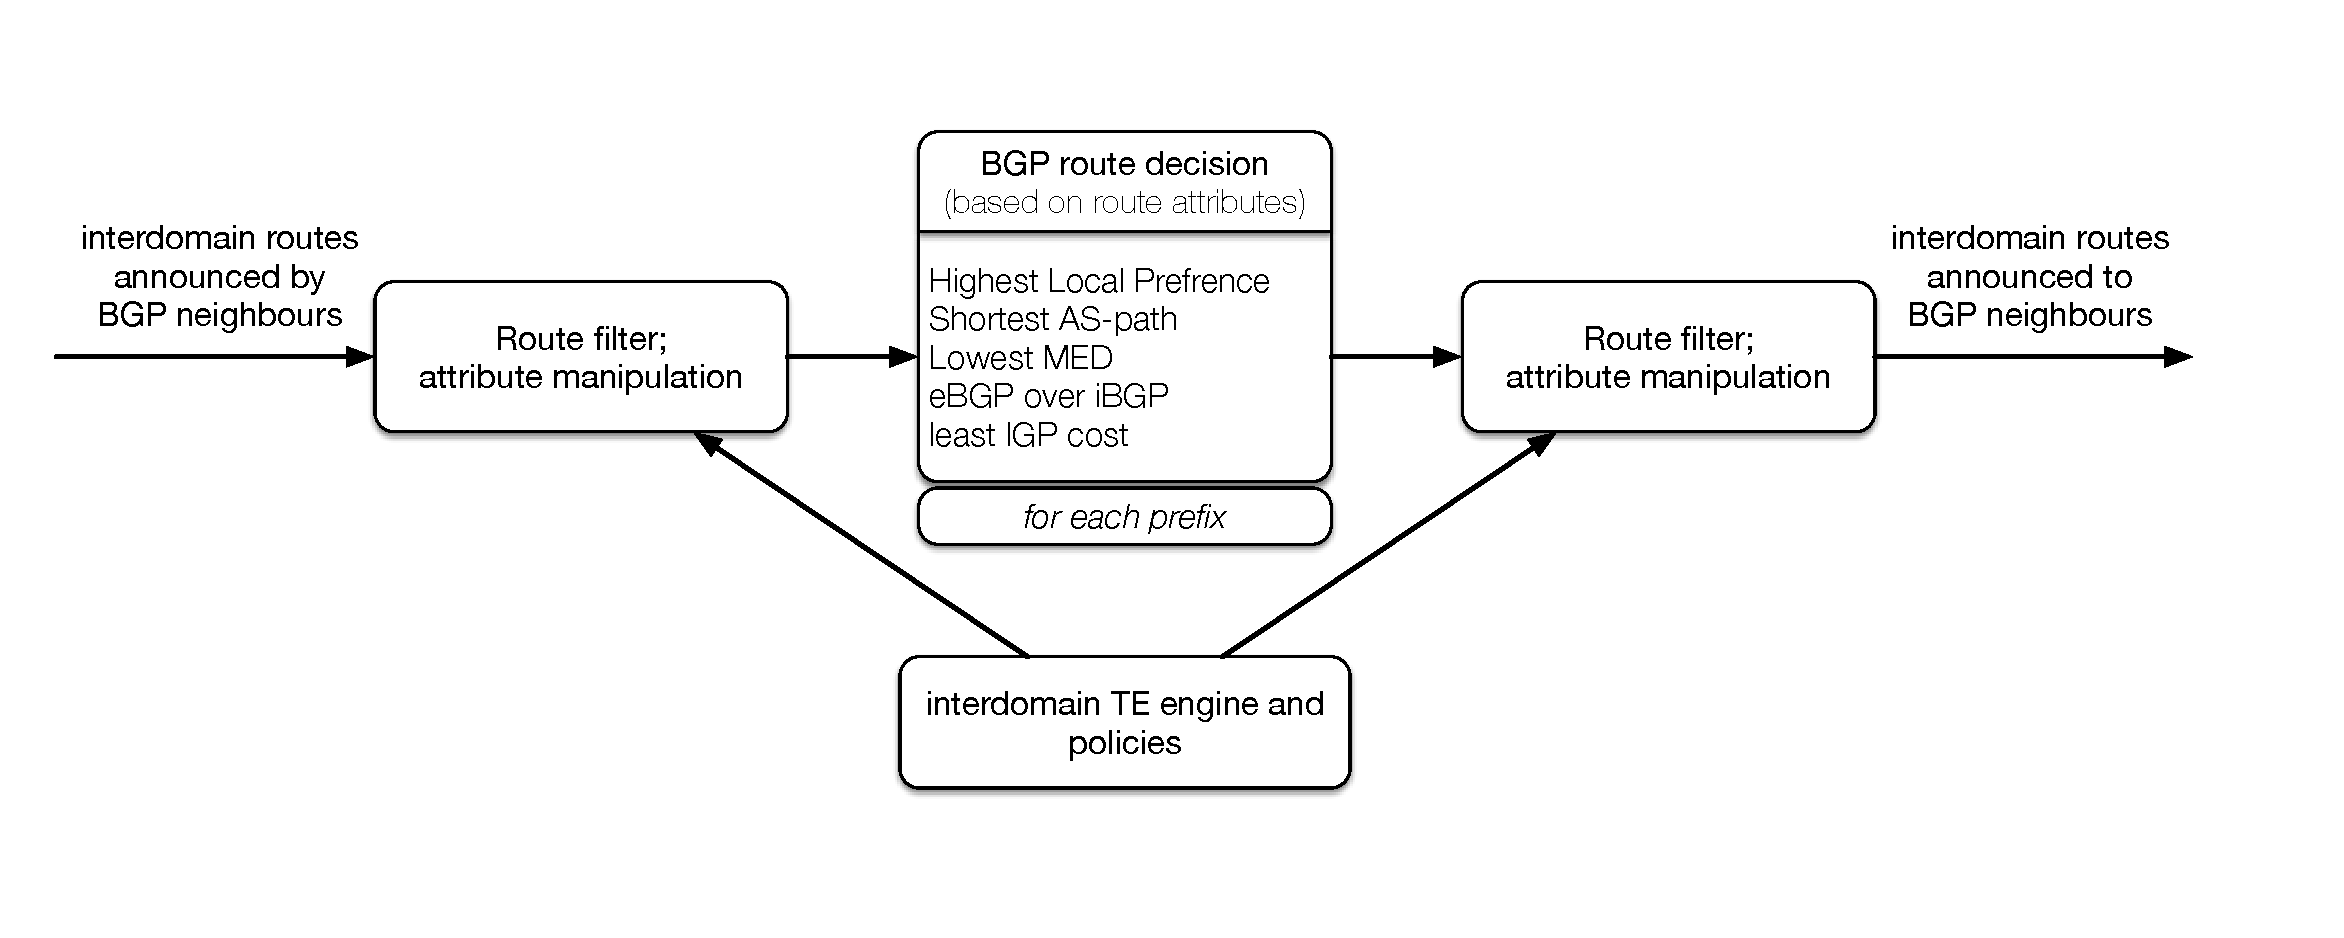
\includegraphics[width=1.3\textwidth]{gfx/chap1/bgp_decision.pdf}
\caption{Workflow of \acf{BGP} route selection and propagation within an \acf{AS}.}
\label{fig:bgp_decision}
\end{figure}

Interconnection of tens of thousands of independently manged networks forms Internet.
Each individual network is as well called an \acf{AS}.
Routing that happens among those ASes is referred to as 
\textit{interdomain routing}.
In order to exchange interdomain routes, each AS uses \acf{BGP}~\cite{bgp4}, a path vector routing protocol, to communicate with other ASes.
Each AS announces its own routes (routes towards its own prefixes) along with other routes to its BGP neighbors.
For each prefix as destination, one single best route is selected by the BGP route decision process.
The selection considers the BGP attributes attached to each route, as illustrated in Figure.~\ref{fig:bgp_decision}.
According to configured TE polices, each route can be filtered or altered based on its attributes~\cite{Quoitin2003, Gao2001a}.
Such operations can take place before BGP route decision and as well before route advertisement to its neighbors.

\begin{figure}[!htb]
\centering
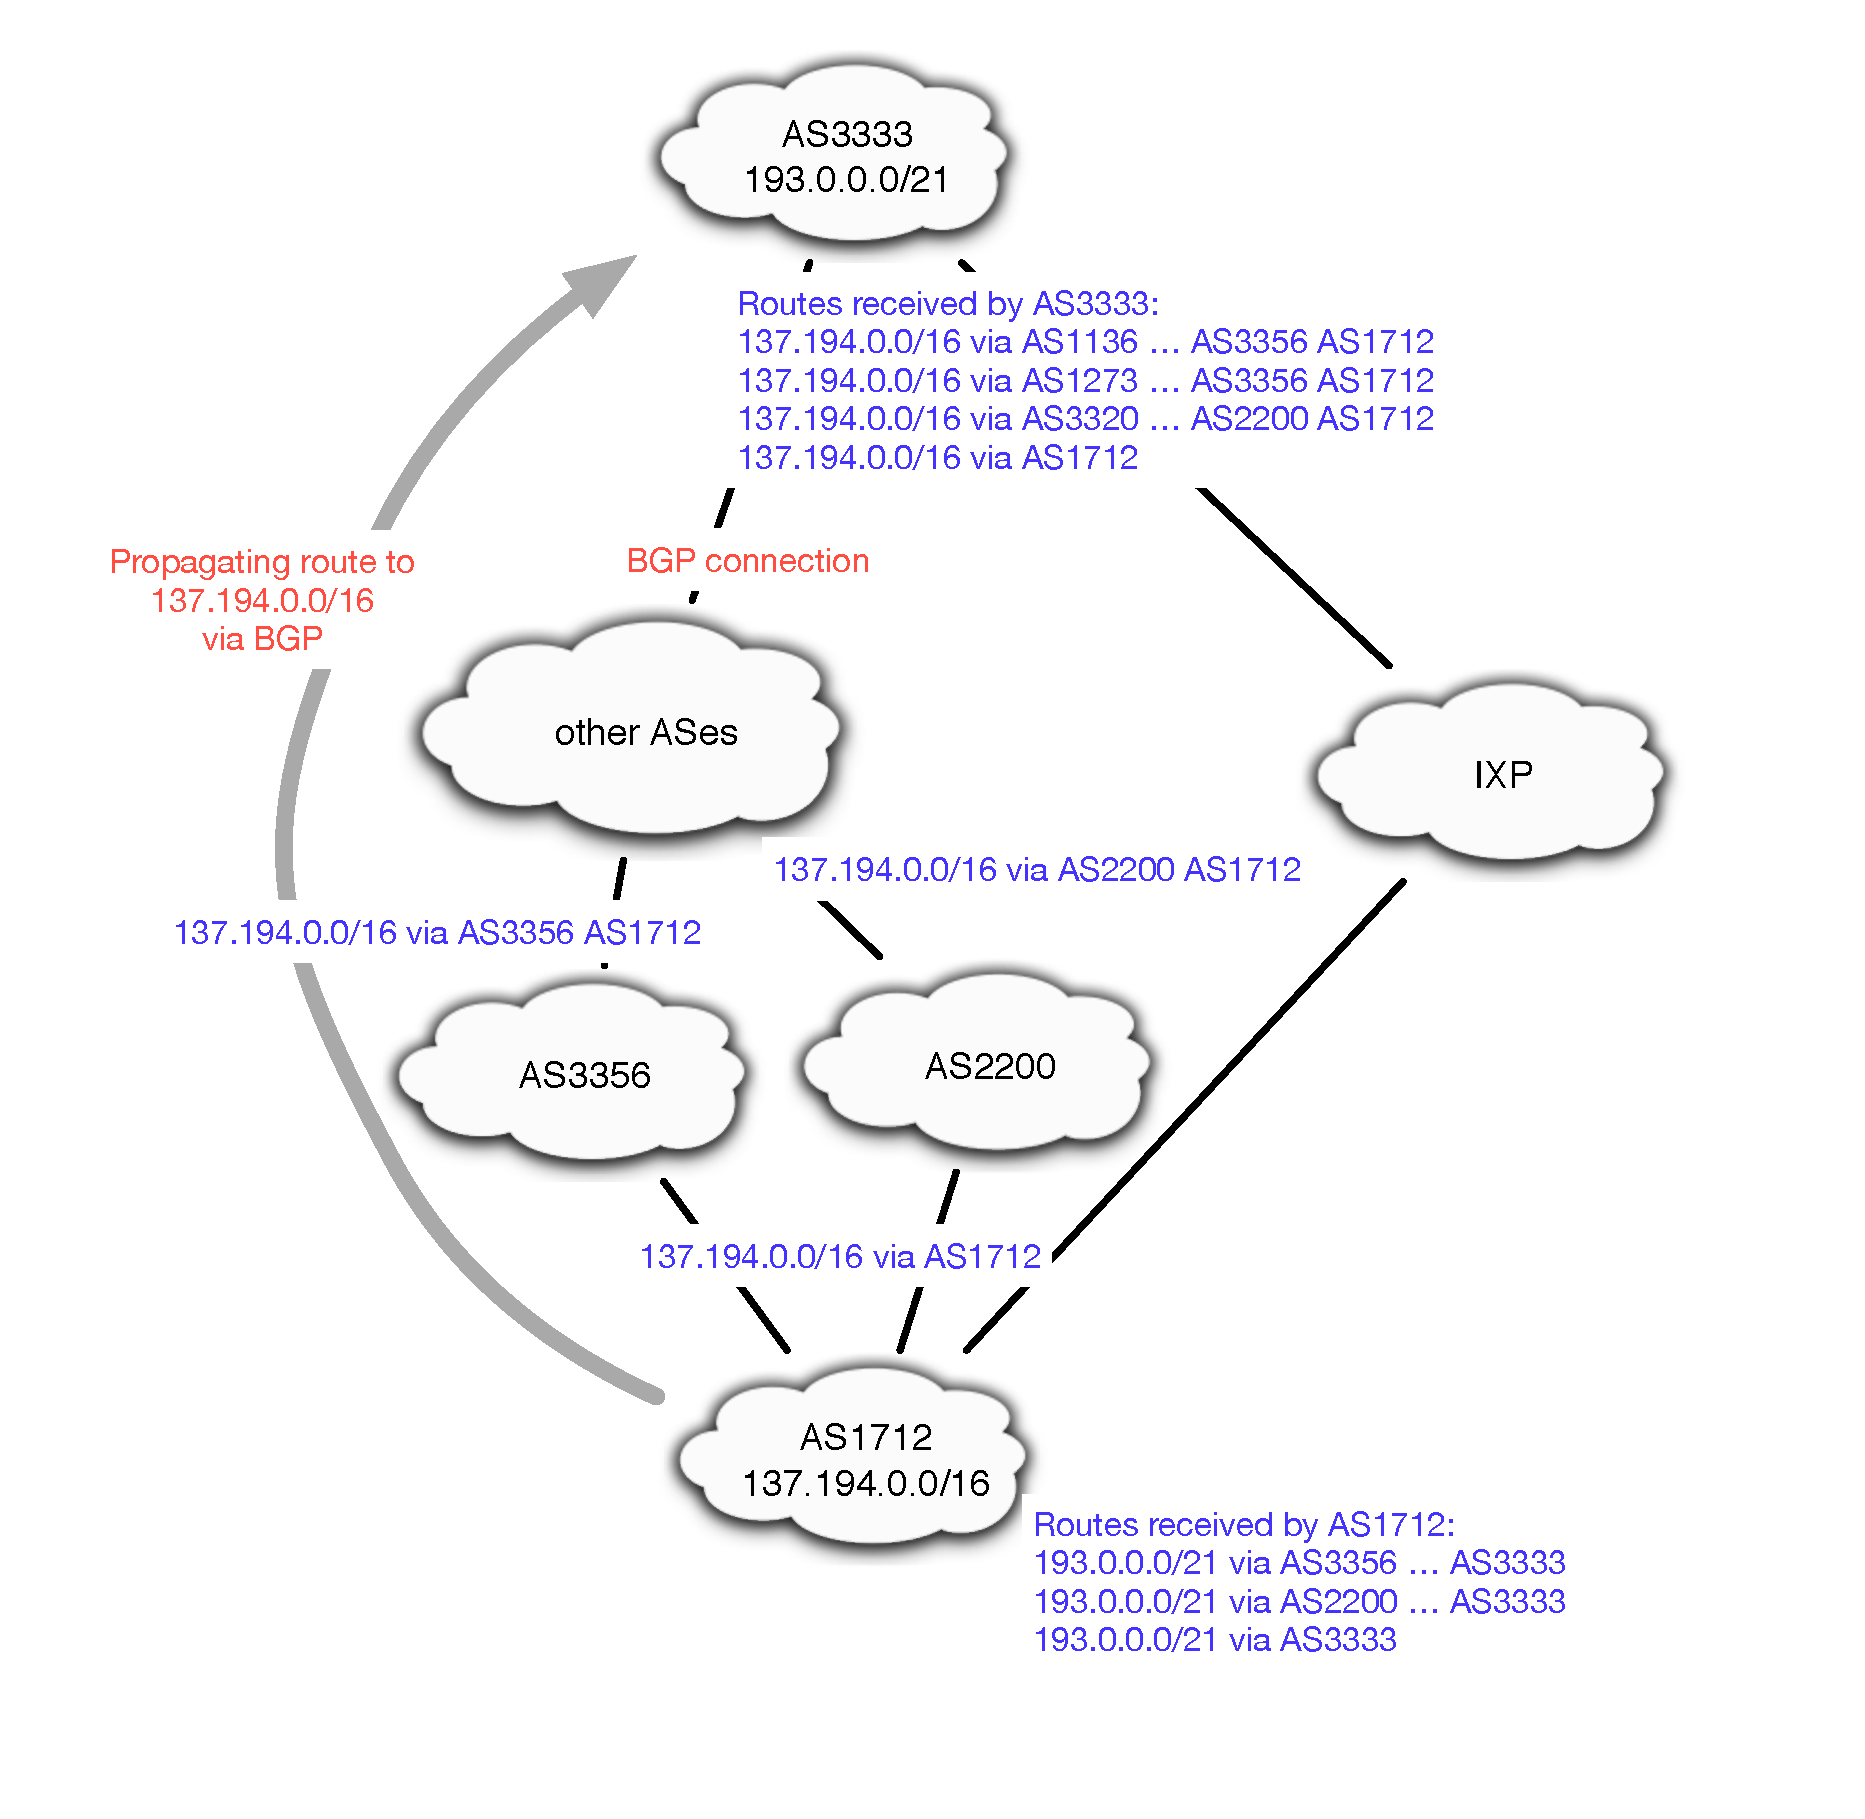
\includegraphics[width=1.1\textwidth]{gfx/chap1/bgp_route_propagation.pdf}
\caption{Interdomain route propagation via \ac{BGP}, an example of \texttt{137.194.0.0/16}. Networks illustrated are fictional.}
\label{fig:bgp_propa}
\end{figure}

Fig.~\ref{fig:bgp_propa} illustrates the propagation of interdomain routes to prefix \texttt{137.194.0.0/16} of AS1712 via BGP exchanges. Each AS inserts its own AS number when announcing the route to other ASes, thus forming an AS path at the receiver side. After AS3333 learns the routes to \texttt{137.194.0.0/16} and AS1712 learns routes to \texttt{193.0.0.0/21} in a similar way, the two ASes can exchange traffic across Internet using these two prefixes.

There are two types of ASes in the above BGP exchanges: \textit{transit provider} and \textit{stub AS}.
Transit provider refers to ASes that offer to route traffic not originated from nor sent to itself, as a commercial service.
For that purpose, a transit provider announces to its clients all the interdomain routes its learns and to its other BGP neighbors the routes to its clients.
In Figure~\ref{fig:bgp_propa}, AS3356 and AS2200 are transit providers of AS1712. They help announce the route to prefix \texttt{137.194.0.0/16}
to the rest of Internet.
On the contrary, a stub AS only cares about sending out its own traffic and becoming reachable to others.
Accordingly, it only announces to its transit providers its own routes. 
AS1712 is a stub AS in Figure~\ref{fig:bgp_propa}, as it does not relay interdomain routes for other ASes. For example, AS1712 will not announce to AS3356 the route to \texttt{193.0.0.0/21} learnt from AS2200. Consequently no traffic toward ASes other than itself shall arrive at it.

Besides the relationship described above, peering is another type of exchange under BGP. Two ASes in peering relationship exchange with each other their own routes, so that they can directly communicate without employing a transit provider.
In Figure~\ref{fig:bgp_propa}, AS1712 and AS3333 directly peer at an \ac{IXP}.
\ac{IXP} is a collocation facility that eases establishment of peering relationship, thus is transparent to BGP route exchanges.

\section{Interdomain TE}
Thanks to transit and peering relationship, AS3333 and AS1712 in Figure~\ref{fig:bgp_propa} may receive multiple routes to send out traffic.
Meanwhile, they may as well receive traffic from multiple neighbors.
Such diversity in route brings up two questions: 1) which routes are the best; 2) how to route corresponding traffic on the desired paths.
The efforts spared in answering these two questions are referred to as \textit{interdomain \ac{TE}}~\cite{Quoitin2004a,Quoitin2003,Feamster2003}.

The first question deals with the objective of \ac{TE}. In general, a network aims at optimizing the cost and/or performance of transmission.
The second question explores the method to steer traffic.
We summarize the current practices, their limitations and challenges for incoming and outgoing traffic separately in this section.

\subsection{Outbound interdomain TE}
%Outbound TE consists in 1) how to identify the best routes for each destination prefix and send out the traffic on these routes 
In sending traffic to a destination prefix, an AS has total control over the routes to be employed. One One common practice is to tune \textit{local preference} BGP attributes~\cite{Wang2008} before BGP route decision (Figure~\ref{fig:bgp_decision}). 
Therefor the challenge is rather on the composition of best routes in terms of cost and performance.

The cost of interdomain transmission depends on the the $95^th$ percentile bandwidth consumption on links purchased from transit providers, i.e. transit links~\cite{drpeering-95th}.
Meanwhile, whether these transit links are congested impacts in return the transmission performance.
Hence, outbound TE resolves in dynamically calculating the appropriate amount of traffic to be routed on each transit link.
The objective of such traffic re-distribution is to lower the overall transit cost, under the constraint of not saturating any transit link at any instant (if possible).

\citet{Goldenberg2004} formulated this quest as a minimum-cost multi-commodity flow problem.
\citet{Uhlig2004b} fulfills the same goal while minimizing the number of route changes by predicting the traffic volume.
\citet{Zhu2014} avoids congestion on transit links by including border router queue length in route decision.

Performance-wise, it is clearly sub-optimal to greedily saturate the cheapest transit link while other transit links remain idle.
However, there are other factors that may as well put transmission performance in danger.
The minimum delay of Internet transmission is dominated by the physical length traversed by a route. 
However, neither AS path length nor transit cost reveals/correlates to the underlying distance.
On top of that, transient events like congestion can as well happen remotely~\cite{Akella2003, Luckie2014}, independent of traffic load on transit links.
To identify performance difference across multiple routes, end-to-end measurements are indispensable.
They cumulatively reflect the contribution along the entire path, including the transit links.


\subsection{Inbound interdomain TE}
Inbound TE takes care of the incoming traffic distribution on available transit links.
Through Figure~\ref{fig:bgp_decision} and \ref{fig:bgp_propa}, we learn that the paths that incoming traffic takes are decided by remote senders.
For instance, AS3333 decides which routes to use to send traffic to \texttt{137.194.0.0/16} of AS1712.
What AS1712 can do to influence the the route decision of AS3333 is to control its route advertisement.
Shown in Figure ~\ref{fig:bgp_decision}, an AS can filter routes or change certain BGP attributes before advertisement.
Some common practices are: selective announcement, more specific announcement, AS path prepending, setting \ac{MED}~\cite{Wang2008}.

These approaches are not perfect. 
Selective announcement introduces reachability risks.
More specific announcement gives rise to \ac{RIB} inflation. 
AS path prepending is shown to be feeble in avoiding a specific ingress link~\cite{Quoitin2004a}. 
BGP community~\cite{Donnet2008, Shao2015} and redistributed communities~\cite{Quoitin2002} allow finer grained operations with better certainty. 
However, it requires the support from transit providers. 

Under BGP, it appears to be very difficult to have a fine control over the paths/ingress links of incoming traffic. 
In this context, many efforts were focused on incoming traffic steering mechanism.
Traffic ingress point can be dictated by setting the source address of outbound traffic to that of the desired ingress interface.
Such address `spoofing' can be achieved through encapsulation~\cite{Liu2008} or \ac{NAT}~\cite{Sun2015}. However, outgoing traffic could be dropped, for security considerations.
Because it seems to come from outside the prefixes that the AS announces\cite{filtering}.
\ac{LISP} pushes such approach to a revolutionary level by introducing a separate addressing space in the core of Internet that enables various TE operations that are impossible with mere BGP~\cite{lisp}. Studies show fine-grained and dynamic inbound optimization is feasible with \ac{LISP}~\cite{Iannone2007, saucez2011mechanisms, quoitin2007evaluating}.
Yet, the protocol deployment remains limited.

\subsection{Software Defined Networking and interdomain TE}
Recently, \acf{SDN} brings as well new possibilities to interdomain TE. 
One idea is to delegate the TE tasks of an AS to a third party.
The third party performs route decision and traffic steering in a centralized manner, in accordance to \ac{SDN} design philosophy.
It is advocated that the interdomain TE can hence be done in a more cooperative way.
Since conflicts of interest involving multiple ASes are solved centrally, an overall optimality can be achieved.
\citet{Kotronis2012} advances that such AS clusters under same TE service provider can form and expand in a gradual way thanks to network effect.
\citet{Gupta2014} focuses on the application of \ac{SDN} in a more specific network environment, \ac{IXP}.
The members of an IXP by nature forms a cluster of ASes.
They exchange their routing information along with their TE polices within one centrally managed facility. 
Application specific peering, e.g. only peer for the exchange of video traffic, is made possible under this framework.

\section{Scope of this thesis}
We stage the works of this thesis under BGP, while fully realizing \ac{LISP}, \ac{SDN} and etc. are promising directions to pursuit.
It is because BGP is still going to be the \textit{de facto} routing protocol of Internet in the foreseeable future.
And the deployment of any new routing mechanism must be incremental.
Before the takeover of anything non-BGP,  BGP is what a majority of ASes have to live with. 
There are thus immediate needs for improvements.

We focus on outbound TE in this thesis.
Inbound TE has been shown to be inherently difficult with BGP, due to lack of effective traffic steering method.

We target stub ASes (potentially multi-homed).
It is because \ac{CP}, \ac{HP} and \ac{ISP}, being major network types among stub ASes, are those who need most outbound TE.
Moreover, dynamic route re-selection in those networks will not cast Internet-wide BGP route convergence issues.

Finally, we assume improving transmission performance is nowadays the major motivation for outbound TE.
Routing traffic across Internet now faces fewer monetary constraints thanks to decreasing transit price~\cite{transitprice, drpeering} and high \ac{IXP} growth rate worldwide~\cite{pchixp}.
Instead, through demand for geographical and topological connection diversity~\cite{Chiu2015}, a performance challenge remains to be addressed.

\section{Measurement-based TE and motivations}
BGP route decision mechanism is unaware of the performance characteristics of candidate paths~\cite{Yannuzzi2005}, as shown in Figure~\ref{fig:bgp_decision}.
Yet, the transmission performance toward a destination varies over different interdomain routes.
\citet{Akella2003} pointed out that bandwidth bottleneck can be within certain transit providers or on the links between remote ASes.
This observation suggests that the choice of transit provide is of relevance to transmission performance.
Further, \citet{Akella2003a} revealed a $30\%$ potential performance gain that an AS could achieve with multi-homing.
%\cite{Akella2004} advocates that this gain is not far away from that of overlay networking.

In order to actually realize this performance gain, dynamic route selection based on performance measurements is required, i.e. \textit{measurement-based TE}.
\citet{Akella2008} presented a demo implementation of a measurement-based TE system.
Only 100 destinations are emulated in this work.
This number is far less from the actually scale that a stub AS might face on a daily base. 
In the work, the best route for each destination is chosen based on the \ac{EWMA} of past \acf{RTT} measurements. 
The results show that the best transmission performance over all destinations is achieved when route decision is made upon last single measurement.
However, considering the noisy nature of \ac{RTT} measurements, such a simplistic approach can lead to overwhelmingly frequent path changes. 
Moreover, treating Internet as a blackbox for delay measurements fails to provide useful and sometimes necessary insight into the underlying network events.
These network events, e.g. path changes and congestion, are the actual causes for significant performance degradation and the reasons of route change.

In order to address the above concerns and narrow down the gap between the concept and a working system~\cite{b6}, 
we study in this thesis traffic volume, delay and path measurements to improve the scalability, measurement interpretation and performance visibility of measurement-based interdomain TE.


\section{Roadmap}
\subsection{Building blocks of measurement-based TE}

\begin{figure}[!htb]
\centering
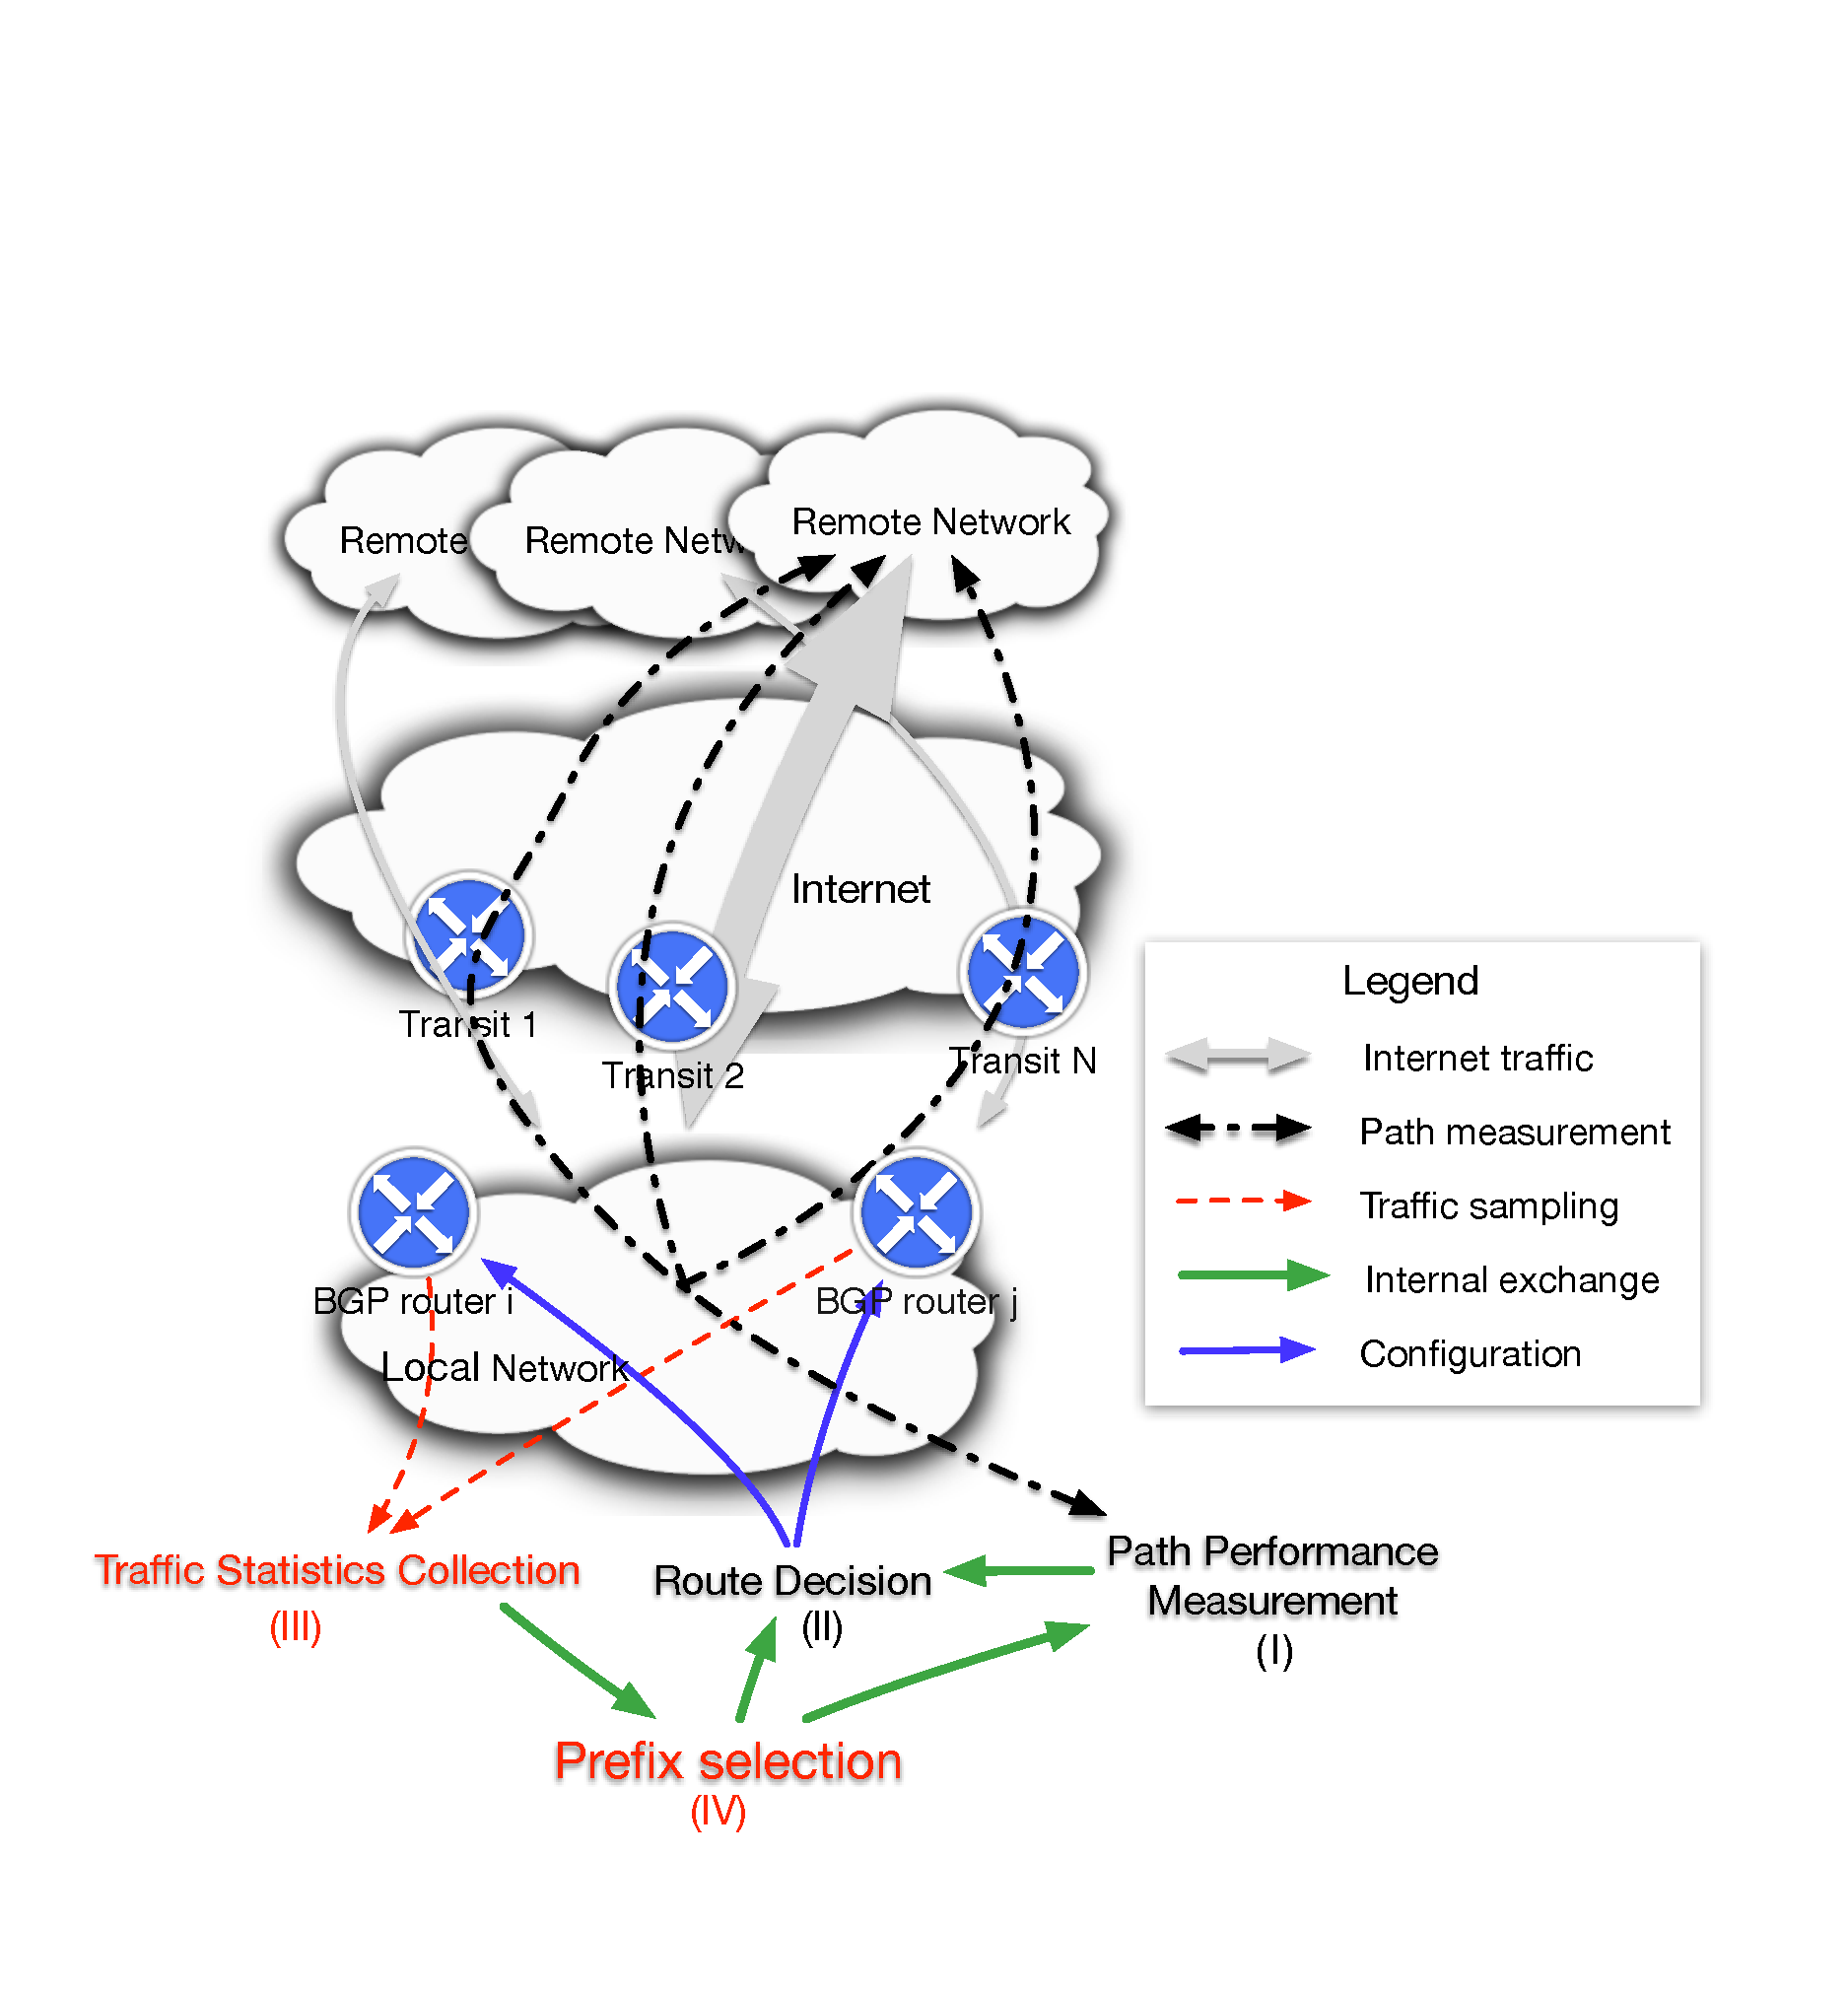
\includegraphics[width=\textwidth]{gfx/chap1/archi.pdf}
\caption{Building blocks of measurement-based inter-domain TE system.}
\label{fig:archi}
\end{figure}

A measurement-based interdomain TE platform has two essential building blocks.
They are illustrated in black in Figure~\ref{fig:archi}: (i) path performance measurement and (ii) route decision.
The platform measures the end-to-end performance, more specifically \acf{RTT}, over all the available routes towards a given destination prefix. 
Within in each destination prefix, a couple of hosts with open ports, e.g. 80, 443, are discovered and then used as probing destination in active delay measurements.
Once fed with performance measurements, route decision engine dictates for each destination the best routes at each moment and imposes them on BGP border routers.

\subsection{Prefix selection: focus on most important destinations}
A scalability issue presents in the above design.
A stub AS can exchange with up to around 100k destination prefixes.
Continuous performance monitoring to all these destinations over all available paths could be prohibitively costly.
\citet{Feamster2003} already realized this issue and proposed to focus on popular destinations.
However, no exact solution was given.
In Chapter~\ref{sec:pref_selec}, we tackle the selection of prefixes associated with important traffic volume.
Through study on their temporal dynamism at different time resolutions, we arrive at very simple yet efficient mechanisms. 
As a part of the proposition, two additional building blocks are added to the system architecture (highlighted in red in Figure~\ref{fig:archi}).

\subsection{RTT measurements with RIPE Atlas}
Studies in Chapter~\ref{sec:pref_selec} base solely on the measurement data collected by a proprietary TE platform~\cite{b6} from client networks. 
Working trace from real networks increases the credibility of our observation. 
However, it brings as well reproducibility concerns.
In Chapter~\ref{sec:ripe_atlas}, we first justify our choice of using RIPE Atlas~\cite{atlas} as source for path and delay measurements in later researches.
We then discuss a data quality issue originated from the measurement platform.

Further, we investigated another data quality issue that is specific to interdomain TE. 
We employ unsupervised learning methods to reveal the inherent structure of a group of delay measurements on a same AS path.

During the above study, we notice an interesting case where several RTT time series exclusively share a similar shape at about the same moment.
We thus find it promising to infer the actually location of shared RTT changes by grouping RTT time series of similar shapes. 
To that end, we study the application of time series clustering methods to RTT measurements and discuss their limitations.

\subsection{Change detection for RTT measurements}
Difficulties in grouping RTT time series with similar shapes leads to further studies in Chapter~\ref{sec:cpt_rtt} and \ref{sec:infer}. 
Chapter~\ref{sec:cpt_rtt} studies the application of \textit{changepoint analysis} methods to RTT measurements. 
These methods aim at detecting significant changes in time series.
We regard the resulted change moment as an expressive way to simplify the representation of RTT time series. 
Meantime, we realize that the detected moments of change can serve as an informative and robust trigger for route re-selection.

To quantify the change detection performance on RTT measurements, we build an evaluation framework and benchmark several candidate methods.
The temporal correlation between RTT changes and routing events are as well studied and illustrated.

\subsection{Inferring the location of RTT changes}
With simplified data representation enabled by changepoint detection, we try to infer the location of detected RTT changes in Chapter~\ref{sec:infer}.
Knowing the location of RTT changes are of significance in measurement-based interdomain TE.
It is especially useful when we hope to optimize the routing to destinations that we are not able to measure directly.
Such network visibility allows avoiding certain problematic paths when end-to-end measurements are absent.

For that purpose, we first group RTT time series undergoing same RTT changes with the help of changepoint analysis.
We come up with a series of inference logic to attribute RTT change to ASes and inter-AS links.
Visualization tools are provided to illustrate the inference process and the inferred locations of change on an AS-level topology.

\cleardoublepage
\chapter{Scalable prefix selection}
\label{sec:pref_selec}

\section*{Abstract}
The growing size of global \acf{RIB} seems to pose a challenge to measurement-based interdomain \acf{TE}. However not all destination prefixes are important to a client network at a certain moment. On average, merely $0.1\% \sim 1\%$ of them are used in forwarding each hour, depending on the network. On top of that, some of them are responsible for much more traffic than the rest, which is known as the highly uneven internet traffic distribution.
Therefore, a nature reflection is to perform TE only for those prefixes that matter.
However, traffic volume associated to a prefix varies over time. And we have little knowledge on the temporal dynamism of traffic across \acf{BGP} prefixes. 
Moreover, it is not trivial predictively identifying prefixes of significance among the crowd, since sophisticated methods predicting volume for each single prefix won't scale in this context.

We revealed in this chapter the relationships among prefix volume importance, stability and predictability basing on working traffic traces from 9 networks of diverse profiles. 
With these findings, we proposed three resource-efficient metrics to predictively select prefixes of important volume. The proposed metrics yielded both satisfying volume coverage and pretty low prefix churn. Furthermore, we showcased that the performance in terms of RTT could differ a lot among different transit providers, which calls for fine-grained dynamic route selection mechanism to drain this gain. The route selection algorithm simulated in the work outperformed the best available transit by $20\%$ on certain networks. 
\clearpage

\section{Prefix selection: a problem of scalability}
\marginpar{what's the problem}
A client network in need of measurement-based interdomain \acf{TE}, often of type \acf{ISP}, \acf{HP}, \acf{CP} and etc., sends out traffic to a wide range of destinations, from several 10k to 100k BGP prefixes.
The measurement and route decision sub-system illustrated in Fig.~\ref{fig:archi} thus faces a scalability issue tracking and optimizing in real time the transmission performance to these destinations.
However, it is well-known that most traffic volume-wide is generally concentrate on only a fraction of the BGP prefixes~\cite{Fang1999, Feamster2003, Papagiannaki2005, Sarrar2012}, 
making it possible and reasonable to focus only on those important destination prefixes in measurement and route re-selection. 

\marginpar{the proposition}
Confine measurement-based TE to important prefixes requires predicting which prefixes will correspond to the most important traffic volumes in the near future.  
To this end, two additional function blocks are added to the system design in Fig.~\ref{fig:archi}): (iii) traffic volume statistics collection; (iv) prefix selection process, which selects the set of the most important prefixes (i.e., the ones with the highest volume in the foreseeable future) and communicates the selected prefix set to measurement and route decision function blocks.

\marginpar{challenges}
Two reasons oblige us to \textit{predictively} select prefixes of important volume and devise specific mechanisms for that task.
First, traffic volume per prefix evolves over time, so does the set of prefixes representing important traffic volume. Walleriche et al.~\cite{Wallerich2006} showed that the bandwidth ranking of a 5-tuple flow can change drastically from one moment to another.
In order to maintain a set of prefixes of importance, one thus has to predict traffic volume for each prefix repeatedly.
To our best knowledge, no study has given an in-depth investigation on the evolution in time of the traffic volume associated with BGP prefixes.

Second, in predicting traffic volume for each individual prefix, more efficient methods are needed.
Well established \acf{TSF} models and \acf{ANN} have been used previously in traffic prediction \cite{Papagiannaki2005, Cortez2006, Otoshi2013}.
These works targeted on highly aggregated inter-\acf{PoP} traffic for off-line tasks, such as network dimensioning.
These models are not only computationally heavy, but also require data pre-processing and parameter tuning to fit well to each individual volume trace, which makes them less applicable in the context of inter-domain TE involving upto some 100k prefixes. Therefore, less complex prediction methods are needed. 


\marginpar{contributions}
The rest of this chapter is organized as following:
\begin{itemize}
\item Section~\ref{sec:chp2_related_work} reviews some related works on Internet traffic dynamism, \ac{FIB} caching and the performance gain of interdomain TE.
\item Section~\ref{sec:chp2_chara} studies mainly the temporal dynamism of Internet traffic at BGP prefix scale with working traffic traces from networks of diverse profiles (\ac{ISP}, \ac{HP} and \ac{CP}) located in different countries (France, Germany, Poland, Spain, UK and USA).
It as well quantitatively describe the burstness of traffic, closely related to predictivity, from each of these client networks. 
\item Section~\ref{sec:sele} proposes three metrics for the prediction of important prefixes based on the findings established in Section~\ref{sec:chp2_chara}. 
These methods are evaluated and compared to Grey model employed in one previous work on \ac{FIB} caching. 
Results show that the proposed schemes out-perform the Grey model in terms of volume coverage and prefix churn. 
\item Finally, the end-to-end path performance through each available transit provider are measured from the nine client networks toward their own selected prefixes of volume importance. The transit provider performance evaluation confirmed former studies on the significant differences among transit providers in multihoming -- highlighting, therefore, that the potential gain of measurement-based interdomain \ac{TE}.
\end{itemize}


\section{Related work}
\label{sec:chp2_related_work}
Some previous works \cite{Feamster2003, Akella2008, Goldenberg2004} acknowledged the importance of performing inter-domain TE only for destinations that truly matter.
However, no general solution was proposed to predictively select the BGP prefixes with important traffic volume.

\marginpar{FIB caching}
Some other works leveraged the skewed distribution of Internet traffic to downsize \ac{FIB}, 
which aims at installing only a small part of the Internet routes, due to some software or hardware limitations~\cite{Iannone2007, Ballani2009, Kim2009, Zhang2012, Sarrar2012, Liu2015}.
In these works, traffic dynamism on much smaller time scales, e.g. seconds and minutes, is of relevance. 
In our work, we used traffic traces of coarser time resolution over longer period of time --- conditions more adapted to the complicated operations required in inter-domain TE, especially path performance measurement.
Nonetheless, we have compared as well our prefix selection methods to these works in the belief that our study could be of value for their problem as well. 

\marginpar{traffic temporal dynamism}
When it comes to the understanding on traffic dynamism, Zhang et al.\ \cite{Zhang2012} assumed that the stability and popularity of Internet traffic is positively correlated without verification. 
Papagiannaki et al.\ \cite{Papagiannaki2004} showed that this correlation is not evident for 5-tuple flows on 5 minute interval. 
Our work studied this relationship for BGP prefixes using working traffic traces collected from networks of diverse profiles.

\marginpar{performance gain of interdomain TE}
Regarding the performance benefit of actually taking advantage of multiple paths in multi-homing, Akella et al.\ \cite{Akella2003a} quantified the performance gain using traces from a large CDN network more than ten years ago. 
In a latter work \cite{Akella2008}, they evaluated a dynamic route selection system on a testbed, but with only 100 destinations. 
We evaluated this gain by performing delay measurements from real client networks toward important prefixes predictively selected with approaches proposed in this article.

\section{Characters of Internet traffic over BGP prefixes}
\label{sec:chp2_chara}
\begin{table}[!tb]
\centering
\setlength{\tabcolsep}{0.5em}
\begin{tabular}{cccccccccc}
\toprule
 & \textbf{SA} & \textbf{SB} & \textbf{SC} & \textbf{SD} & \textbf{SE} & \textbf{SF} & \textbf{SG} & \textbf{SH} & \textbf{SI} \\
\midrule
\textbf{Type} & CP & ISP & HP & HP & CP & CP & ISP & CP & HP \\
\textbf{Vol.} & 133 & 528 & 6.7 & 1129 & 1871 & 5.1 & 0.2 & 29.9 & 6.2 \\
\bottomrule
\end{tabular}
\caption{Average traffic volume per hour (in GB) for the different measured networks}
\label{tab:network_type}
\end{table}

\marginpar{dataset}
We base our study on working traffic traces collected from 9 client networks of very different profiles listed in Table~\ref{tab:network_type}. 
They are either \ac{CP}, \ac{HP} or \ac{ISP}. 
Traffic traces covers a time period of two entire weeks, from May 25th, 2015 to June 8th, 2015, from all networks except SB and SD, for which the traces only cover the second week (starting from June 1st, 2015).
These traces were sampled from real traffic, similarly to previous works concerning FIB caching \cite{Kim2009, Zhang2012}.
It has been shown that the bias introduced by sampling is negligible especially when we focus on large volume prefixes.

\marginpar{time bin size}
Traffic volume toward each BGP prefix is cumulatively bucketed in 1 hour bins.
In comparison, studies concerning FIB caching \cite{Sarrar2012, Zhang2012} use shorter time bins, from 1 second to 10 minutes, to capture instant variations of traffic characters.
In our case, we argue that 1 hour is an appropriate update interval for 
prefix selection, as each prefix selection round is followed by time consuming operations, e.g. finding reliable hosts cane be actively probed within a newly selected prefix. 
%Moreover, changing the set of popular prefixes too frequently might lead to BGP route changes and cause packet re-ordering.

\subsection{Traffic distribution over BGP prefixes}
\label{sec:dis}

\begin{figure}[!th]
\centering
        \begin{subfigure}[b]{0.49\textwidth}
				\centering
                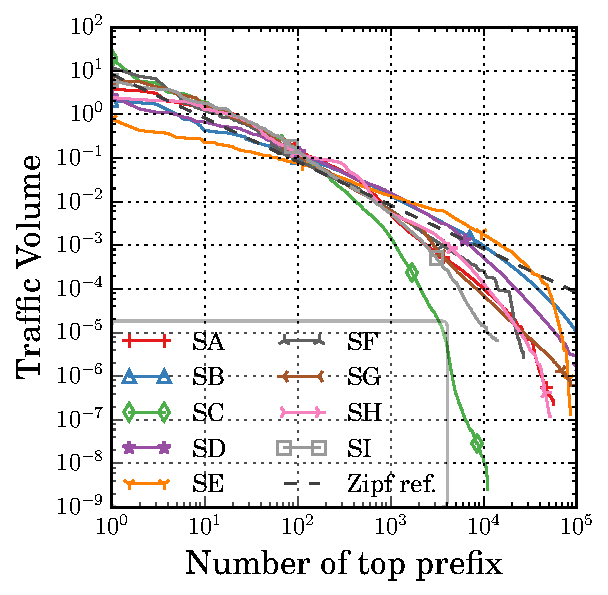
\includegraphics[width=\textwidth]{gfx/chap2/loglog_multi_site.pdf}
                \caption{Week volume share, log-log.}
                \label{fig:week_zipf}
        \end{subfigure}  
        \hfill
        \begin{subfigure}[b]{0.49\textwidth}
        		\centering
                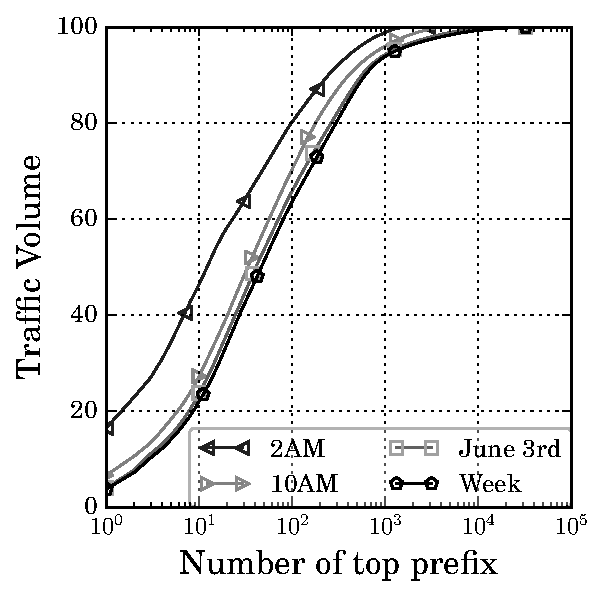
\includegraphics[width=\textwidth]{gfx/chap2/cdf_multi_time.pdf}
                \caption{CDF, different time spans, SA.}
                \label{fig:sa_cdf_multi_time}
        \end{subfigure}    
\caption{Traffic distribution among BGP prefixes.}\label{fig:traffic_dis_site}
\end{figure}

As outlined earlier, the feasibility of prefix selection is based on the fundamental assumption that most traffic concentrates on a few popular destinations, as some previous work have shown \cite{Fang1999,Feamster2003, Wallerich2006}. We showcase that our dataset demonstrates as well this property of uneven traffic distribution across destination prefixes.

In Fig.~\ref{fig:week_zipf}, the volume share of each BGP prefix is plotted for the week starting from June 1st.
Prefixes are decreasingly sorted along the X-axis according to their cumulative volume fraction over the week.
We observe that the week volume associated with BGP prefixes can be approximately described by a reference Zipf's distribution with $N=10^5, s=1$ (dashed line).\footnote{Zipf's law defines that the $k^{th}$ most popular element among total $N$ elements has an occurrence share of $f(k,s,N)=\frac{1/k^s}{\sum_{n=1}^{N}1/n^s}$.} 
%Wenqin: If this footnote is removed, I'm afraid that the N and s become unclear to readers.
Fig.~\ref{fig:sa_cdf_multi_time} compares the traffic distribution of SA at different time resolution: volumes within one hour time (at 2AM and 10AM), traffic accumulated over 24 hours (on June 3rd) and that through out the full week.
As expected, these graphs confirm that Internet traffic is highly concentrated on a few prefixes over multiple different time resolutions, even after years of rapid RIB increase~\cite{potaroo}.
However, Fig.~\ref{fig:sa_cdf_multi_time} demonstrates that the level of traffic concentration over BGP prefixes is not stable but rather varies within a day, for example the $1^{st}$ ranking prefix at 2AM represents almost $20\%$ of all traffic, while at other time or time spans, this ratio is much lower. This observation leads to the study in the following section.

\subsection{Temporal dynamism of traffic over BGP prefixes}
\label{sec:dyna}

\subsubsection{Coefficient of Variation}

Each destination prefix $P$ ever active during a week is associated with a time series $v(P)={\left\{ v(P)_h\right\} }_{h=1, \dots, 168}$ that
stores its traffic volume over the week at hour interval. 
We define the Coefficient of Variation ($c_v$) for prefix $P$'s hour volume series over the week as
\begin{equation*}
c_v(P) = \frac{\delta(v(P))}{\mu(v(P))},
\label{eq:cv}
\end{equation*}
where $\delta$ denotes the standard deviation of the hour volume series and $\mu$ is the mean hour volume over the week.
$c_v$ is a measure of traffic volume variation in relation to its hourly mean over a week.
A large $c_v(P)$ value indicates a large range of variation w.r.t. its average level, and consequently more difficult to anticipate the traffic volumes for this prefix $P$~\cite{He2005}.\footnote{By construction, the maximum $c_v$ for a hourly volume series of 168 in length is $\sqrt{167}$, corresponding to the case where the prefix in question is active during only one single hour throughout the entire week.}

\begin{figure}[!htb]
\centering
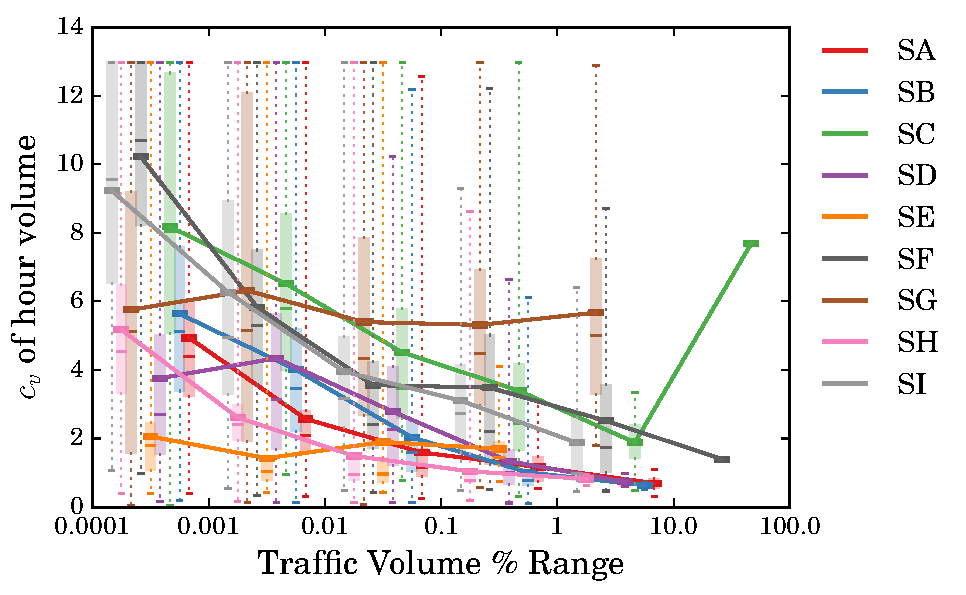
\includegraphics[width=1\textwidth]{gfx/chap2/cv_bin.pdf}
\caption{Relation between $\{c_v(P)\}_P$  and  week volume share for all BGP prefixes $P$. 
}
\label{fig:cv}
\end{figure}

Fig.~\ref{fig:cv} depicts the relation between the coefficient of variation and the volume ``importance'' of the prefix over a week. For each prefix $P$,  the X-axis corresponds to its fraction of volume over the week, grouped in six bins in percentage: $[10^{-4}, 10^{-3})$, $\dots$, to $[10,100)$. Along the Y-axis, we use a  box-plot to describe the $c_v$ distribution for prefixes within each bin, mean, median, 25-75 percentile.
We observe that, for all the networks except SG and SE, $c_v$ of large volume prefixes tends to be smaller in average and constrained in a narrower box. On the contrary, the prefixes with smaller week volume share tend to have larger coefficient of variation. 
This is an interesting property, as it allows us to capture a significant part of the overall traffic (represented by these stable prefixes) by simply selecting the prefixes with large average hour volume. 

\subsubsection{\textit{Core} presence intensity}

We describe traffic dynamism from another perspective:
for each hour $h$, we define the $core_h$ as the set containing top prefixes that represent $95\%$ of total traffic. 
Table~\ref{tab:core_size} lists the average number of prefixes included in the \textit{core} and its percentage with regard to the average number of active prefixes each hour. 

\begin{table}[!htb]
\centering
\begin{tabular}{cccc}\toprule
\textbf{Name} & \textbf{Avg. prefix \#} & \textbf{$\%$ w.r.t active prefix} & \textbf{Max prefix \#}\\
\midrule
SA & 629  & 17.87  & 1051\\
SB & 5264 & 9.45  & 13934\\
SC & 73  & 4.59    & 177\\
SD & 2481  & 17.35 & 3757\\
SE & 15501  & 53.61 & 20900\\
SF & 377  & 30.73    & 772\\
SG & 570 & 7.76    & 1766\\
SH & 965  & 19.42   & 1731\\
SI & 175  & 21.00    & 415\\
\bottomrule
\end{tabular}
\caption{Core prefix set statistics.}
\label{tab:core_size}
\end{table}

If a prefix is inside the \textit{core} at a certain hour, it can be regarded important for bringing a significant amount of traffic.
We thus defined the ``\textit{core} presence'' for a prefix $P$ at each hour $h$ as:
\begin{equation*}
cp(P)_i = \begin{dcases*}
        1  & when $P \in$ $\textit{core}_i$,\\
        0 & otherwise,
        \end{dcases*}
\label{eq:cp}
\end{equation*}
% $cp(P)$ is a time series with which we can further describe the frequency or likelihood of prefix being present in the \textit{core} over the week: 
The \textit{core} presence intensity over one week $I_{cp}(P, 168)$ is then defined as:
$I_{cp}(P,168) = \frac{1}{168} \sum_{i=1}^{168} cp(P)_i$.

\begin{figure}[!tb]
\centering
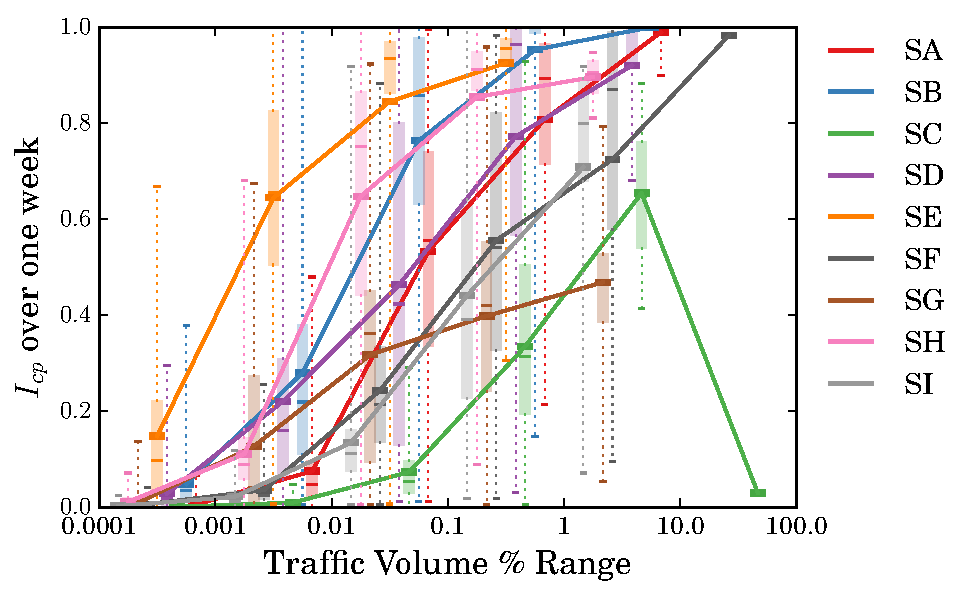
\includegraphics[width=1\textwidth]{gfx/chap2/cp_bin.pdf}
\caption{Relation between $I_{cp}$ over the week and week volume fraction of BGP prefixes.}
\label{fig:cpi}
\end{figure}

Fig.~\ref{fig:cpi} plots the $I_{cp}$ over one week of each prefix (Y-axis) against its week volume fraction (X-axis), using the same presentation as Fig.~\ref{fig:cv} described above.
For all the networks, we can see that prefixes with bigger week volume share are less likely to have a low $I_{cp}$ over the week, i.e. they appear frequently in the \textit{core}.
We can conclude that, by focusing on prefixes that intensively appear in the \textit{core} through the week, we will be able to capture a large part of the prefixes associated with important traffic volume over the week, and thus cover a large part of the overall traffic.

\subsubsection{Relationship between $I_{cp}$ and $c_v$}
\begin{figure}
		\centering
        \begin{subfigure}[b]{0.49\textwidth}
                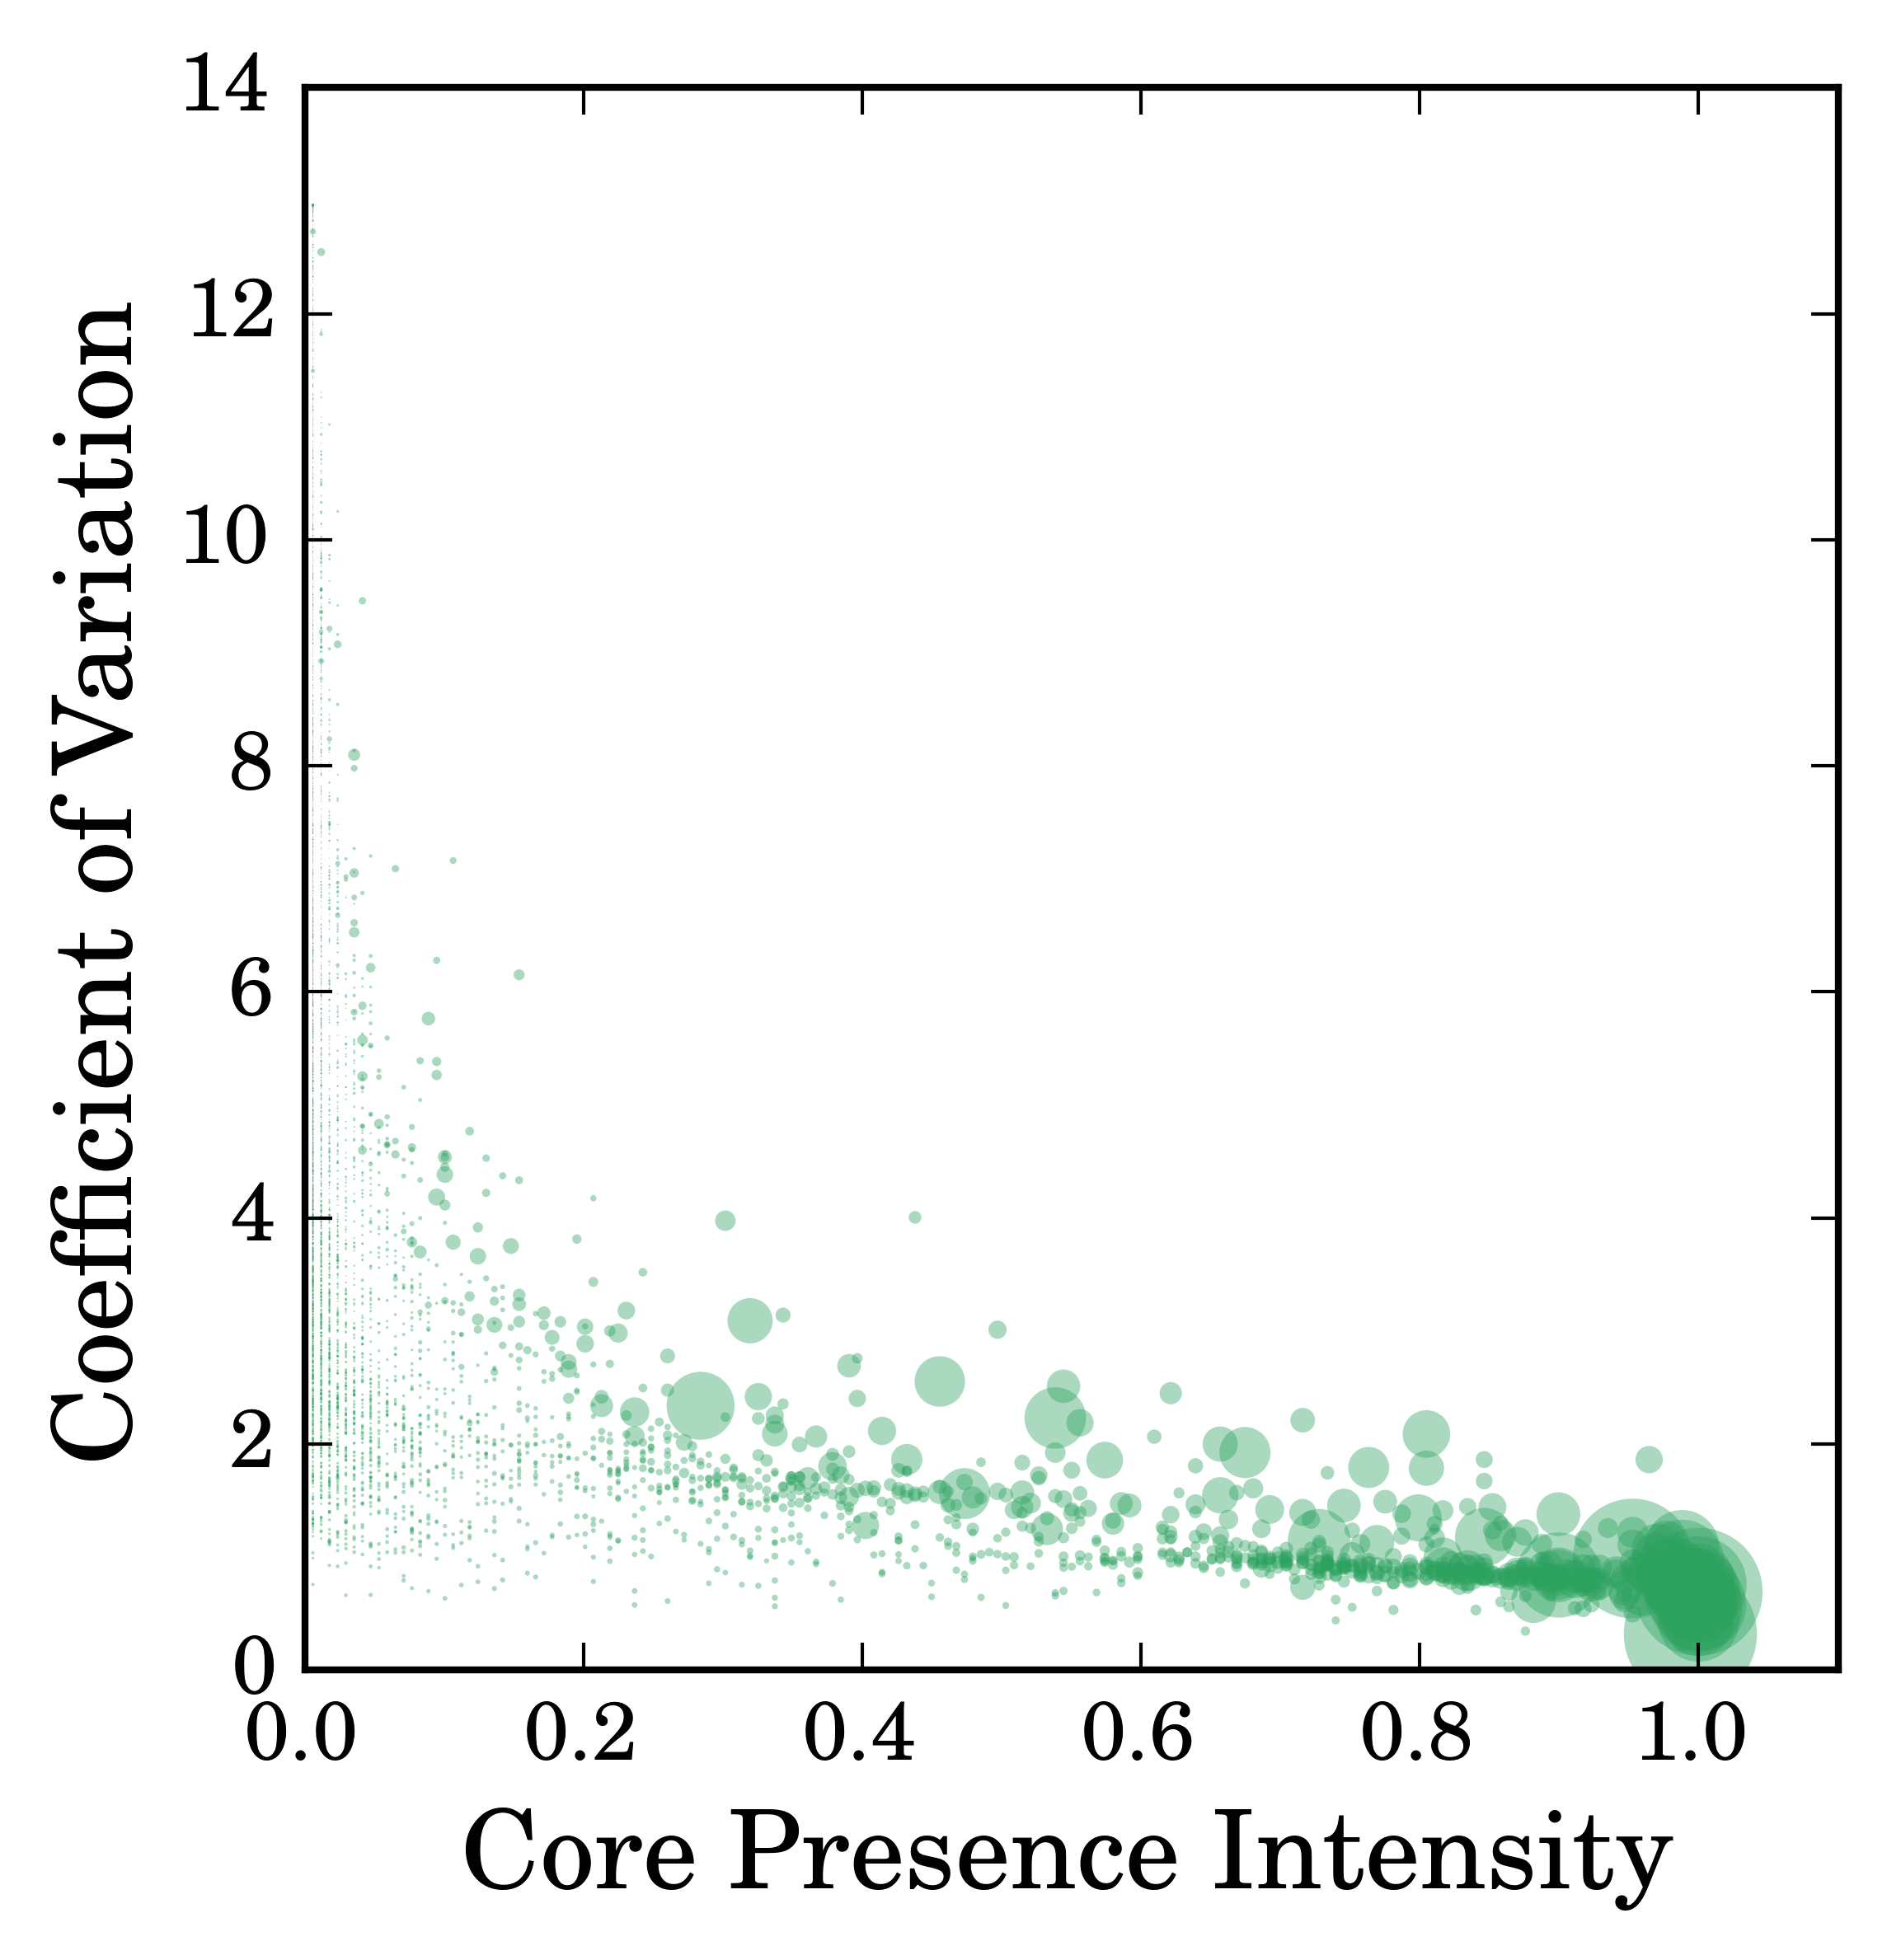
\includegraphics[width=\textwidth]{gfx/chap2/corre_cv_cp_sa.png}
                \caption{SA, 56684 prefixes}
                \label{fig:cv_cp_sa}
        \end{subfigure}
        \begin{subfigure}[b]{0.49\textwidth}
                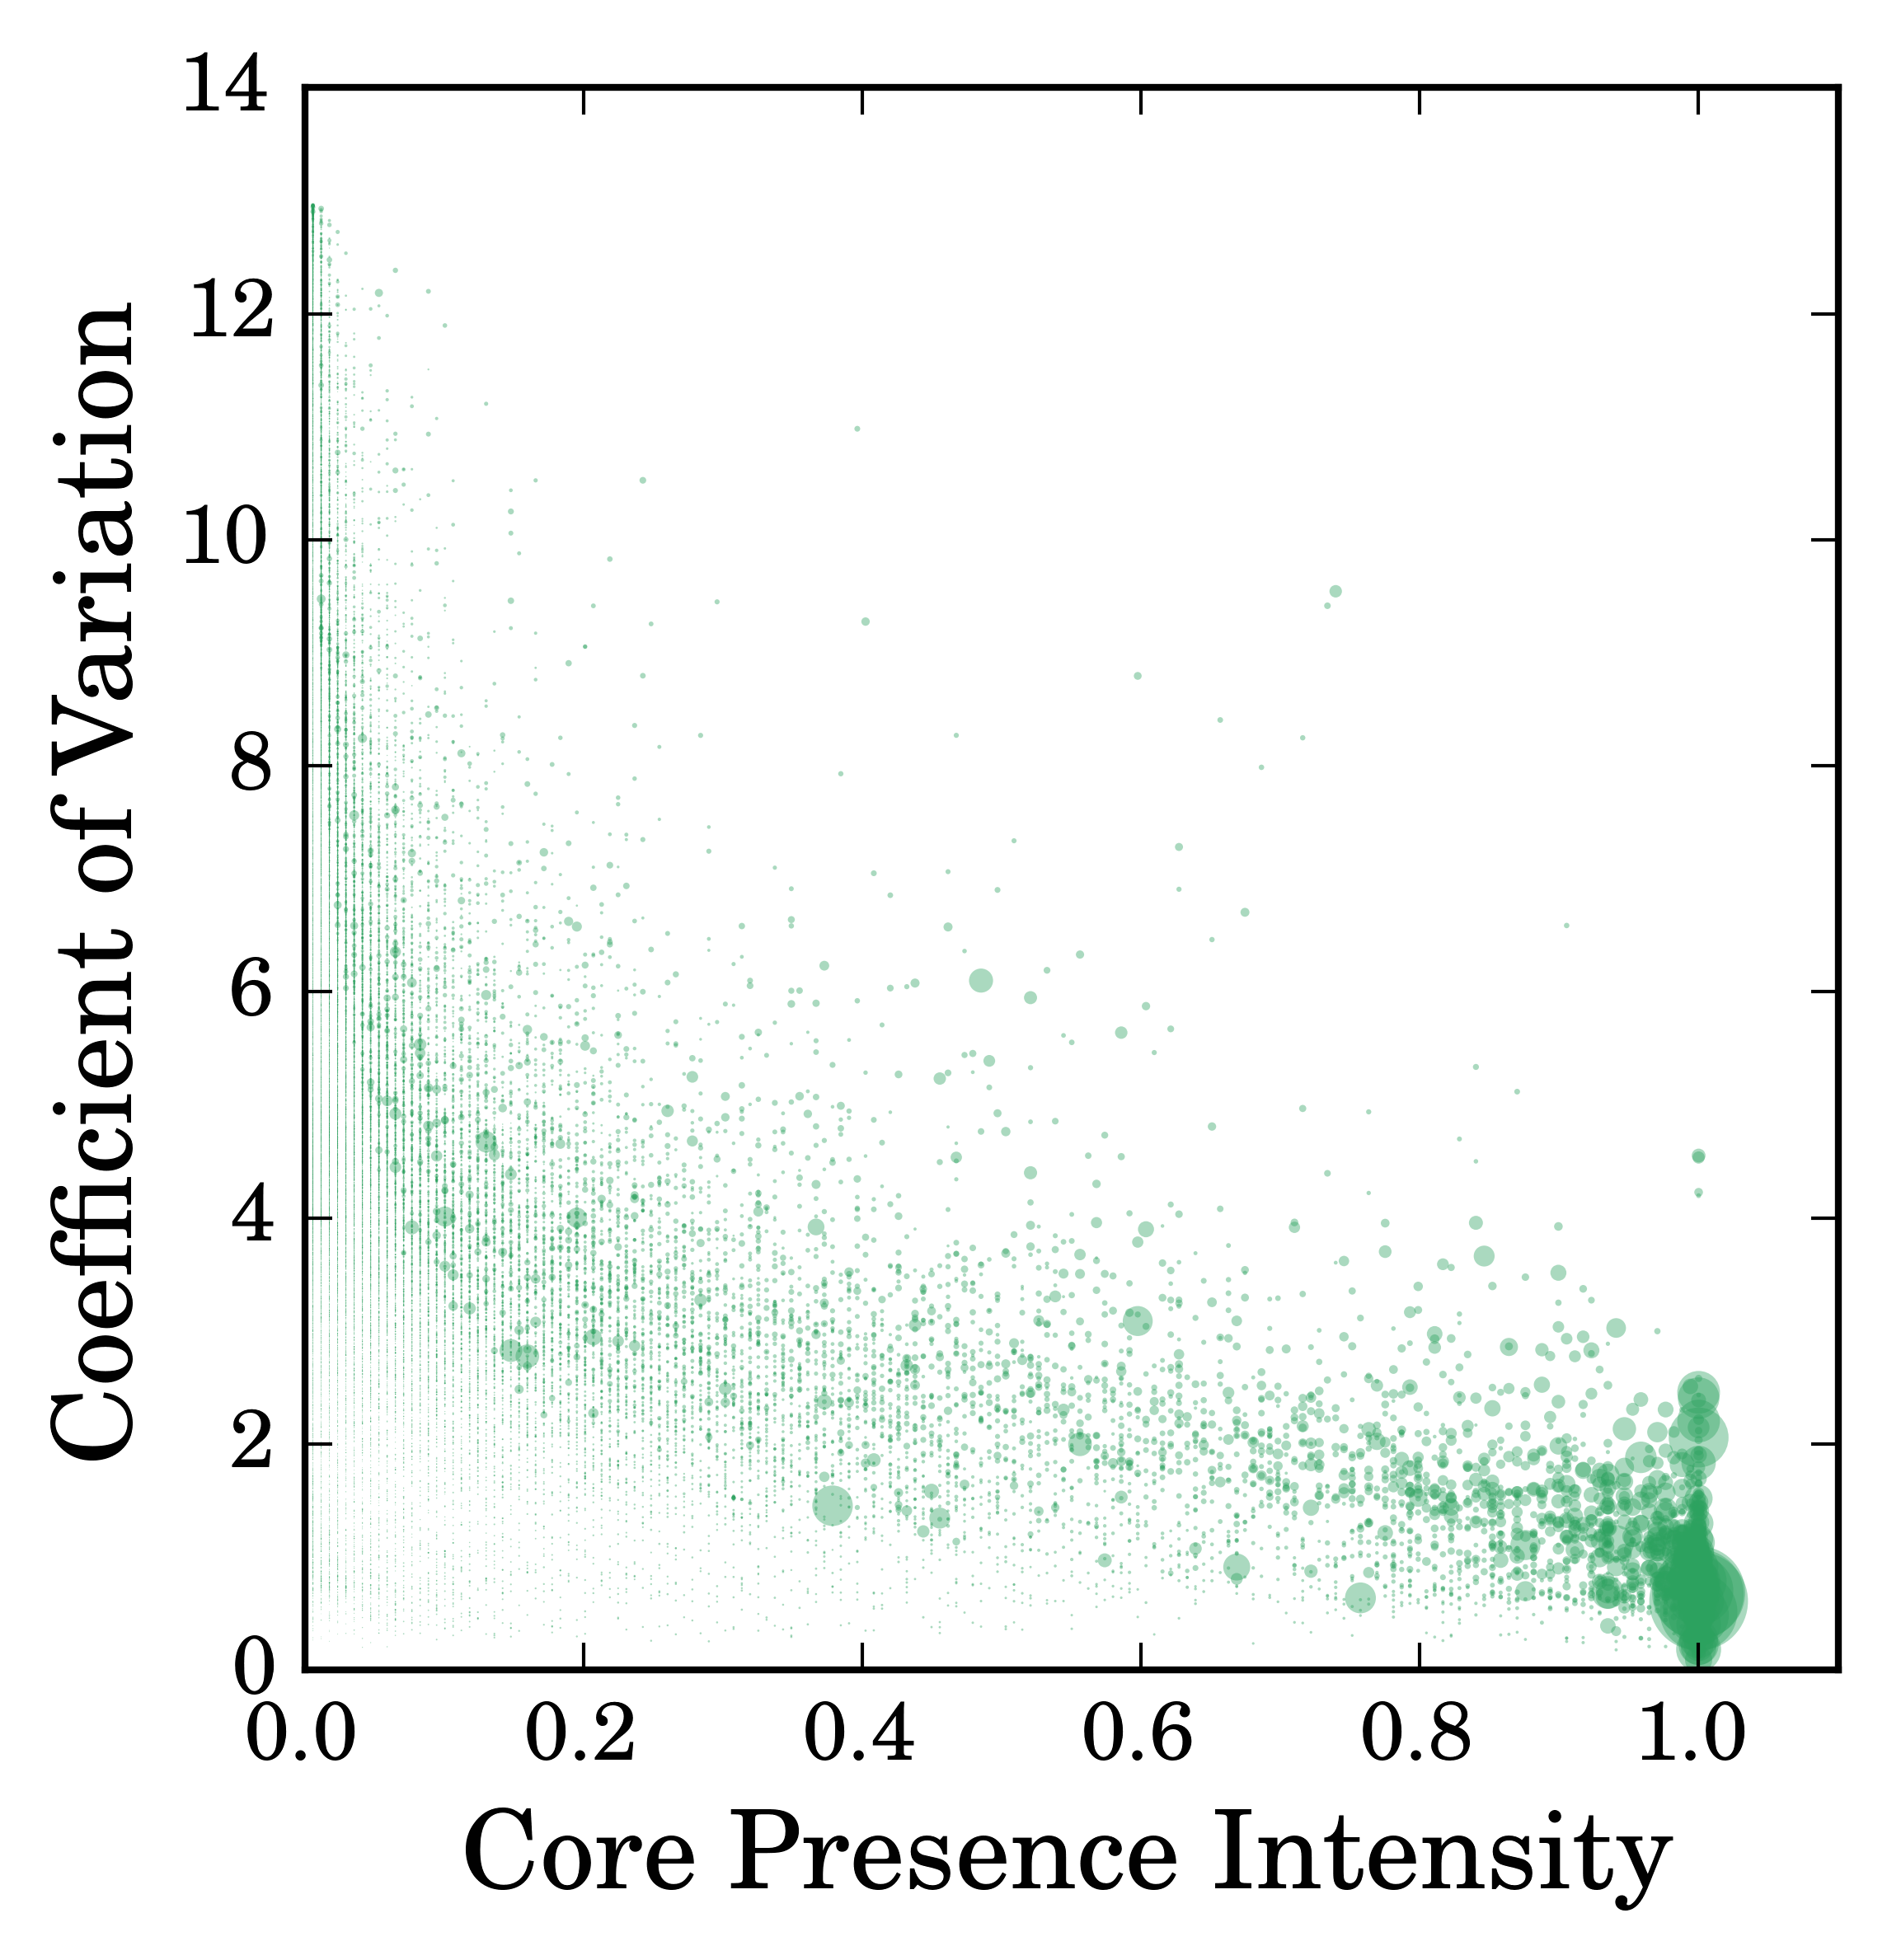
\includegraphics[width=\textwidth]{gfx/chap2/corre_cv_cp_sb.png}
                \caption{SB, 504707 prefixes}
                \label{fig:cv_cp_sb}
        \end{subfigure}
        \begin{subfigure}[b]{0.49\textwidth}
                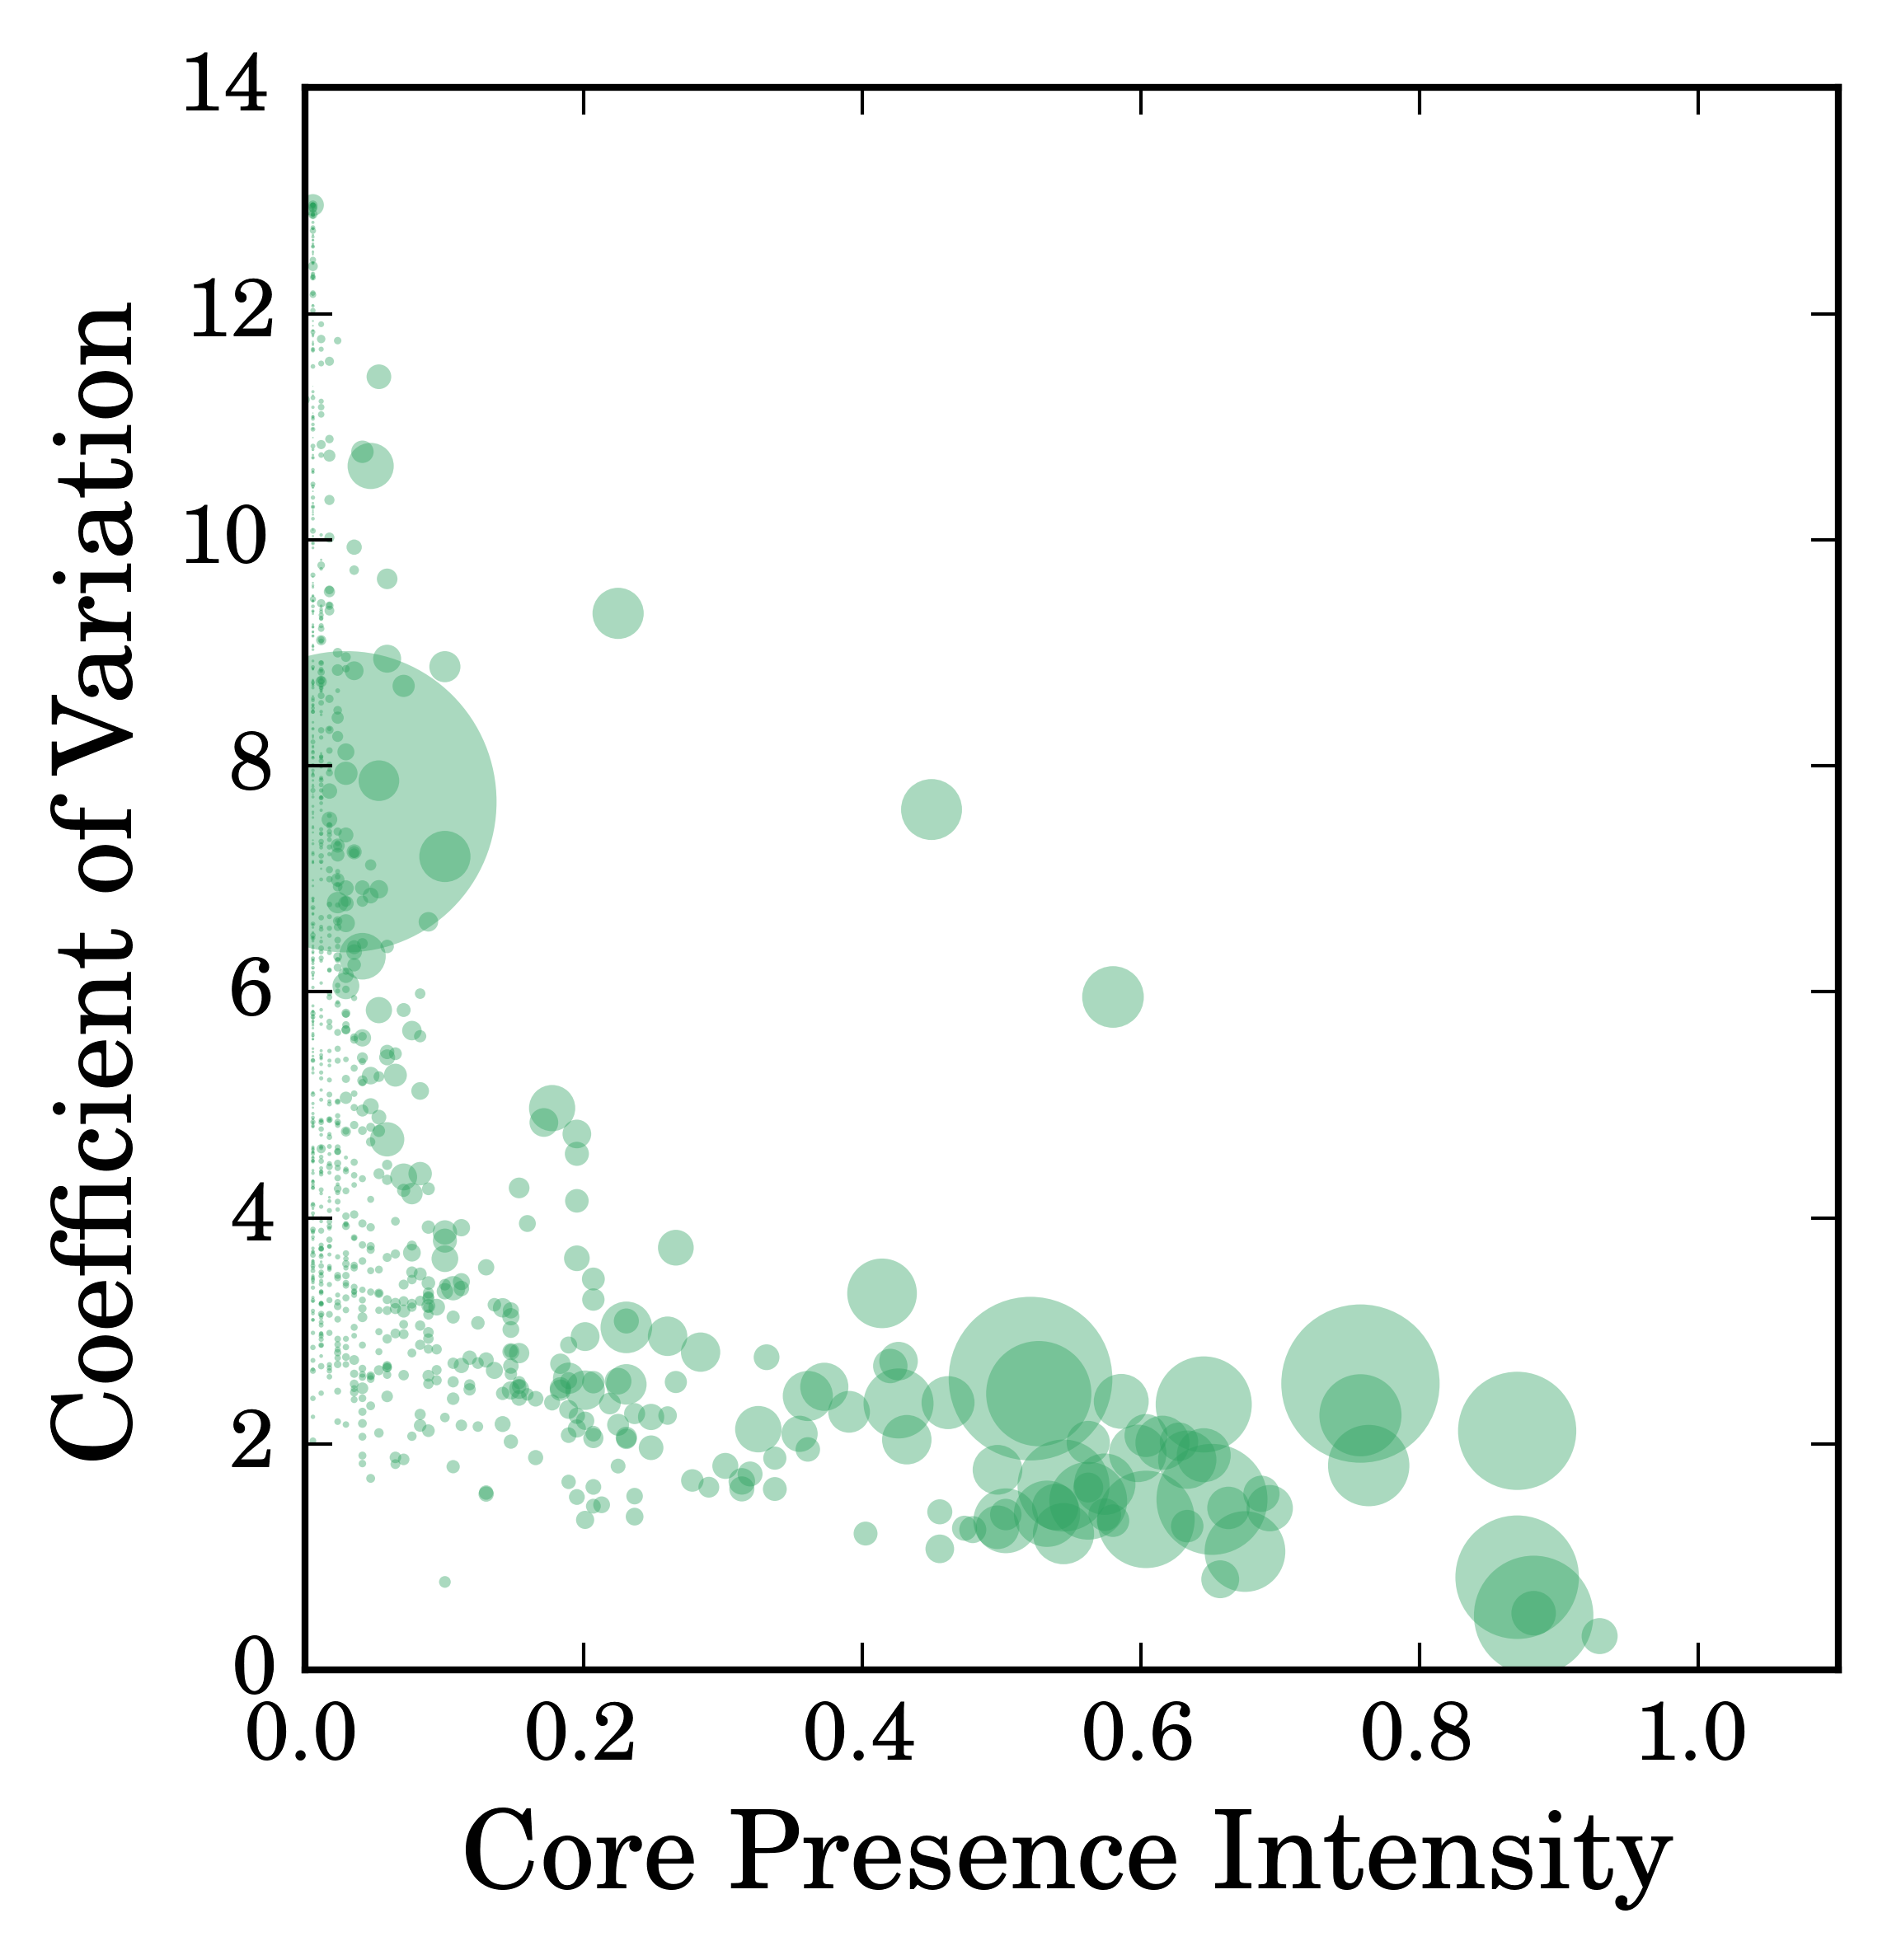
\includegraphics[width=\textwidth]{gfx/chap2/corre_cv_cp_sc.png}
                \caption{SC, 11065 prefixes}
                \label{fig:cv_cp_sc}
        \end{subfigure}
        \begin{subfigure}[b]{0.49\textwidth}
                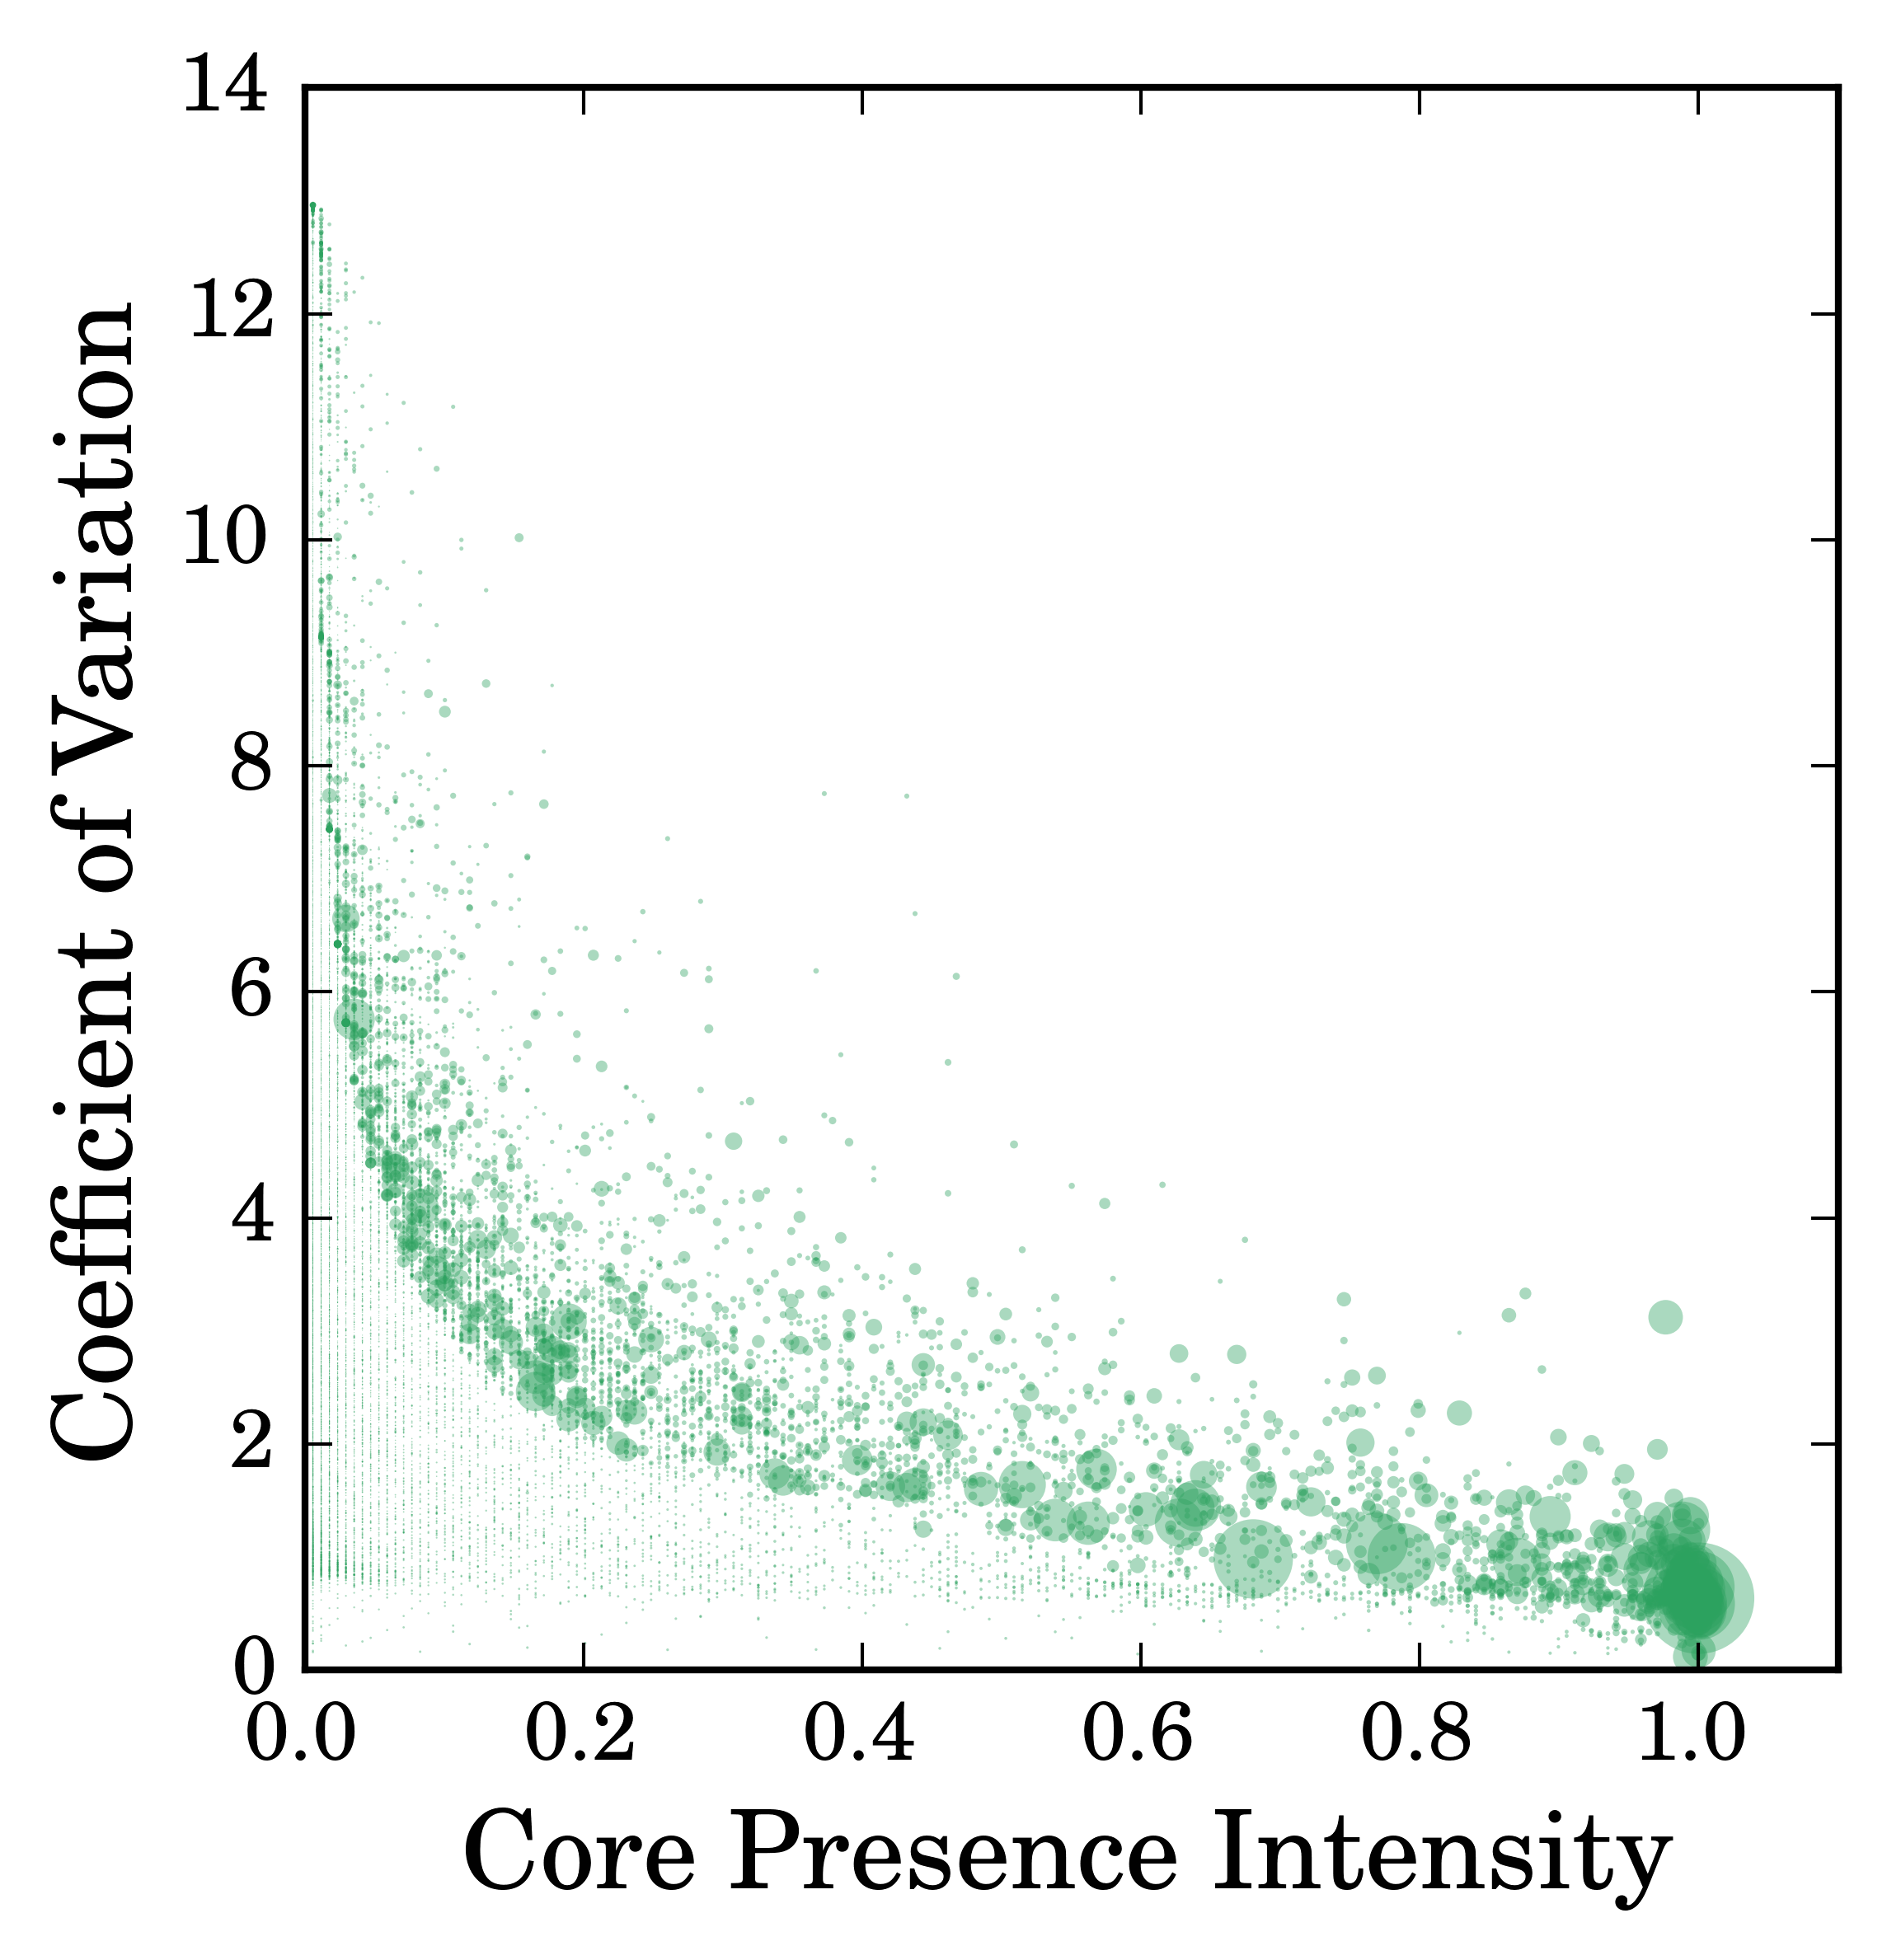
\includegraphics[width=\textwidth]{gfx/chap2/corre_cv_cp_sd.png}
                \caption{SD, 140700 prefixes}
                \label{fig:cv_cp_sd}
        \end{subfigure}
        \begin{subfigure}[b]{0.49\textwidth}
                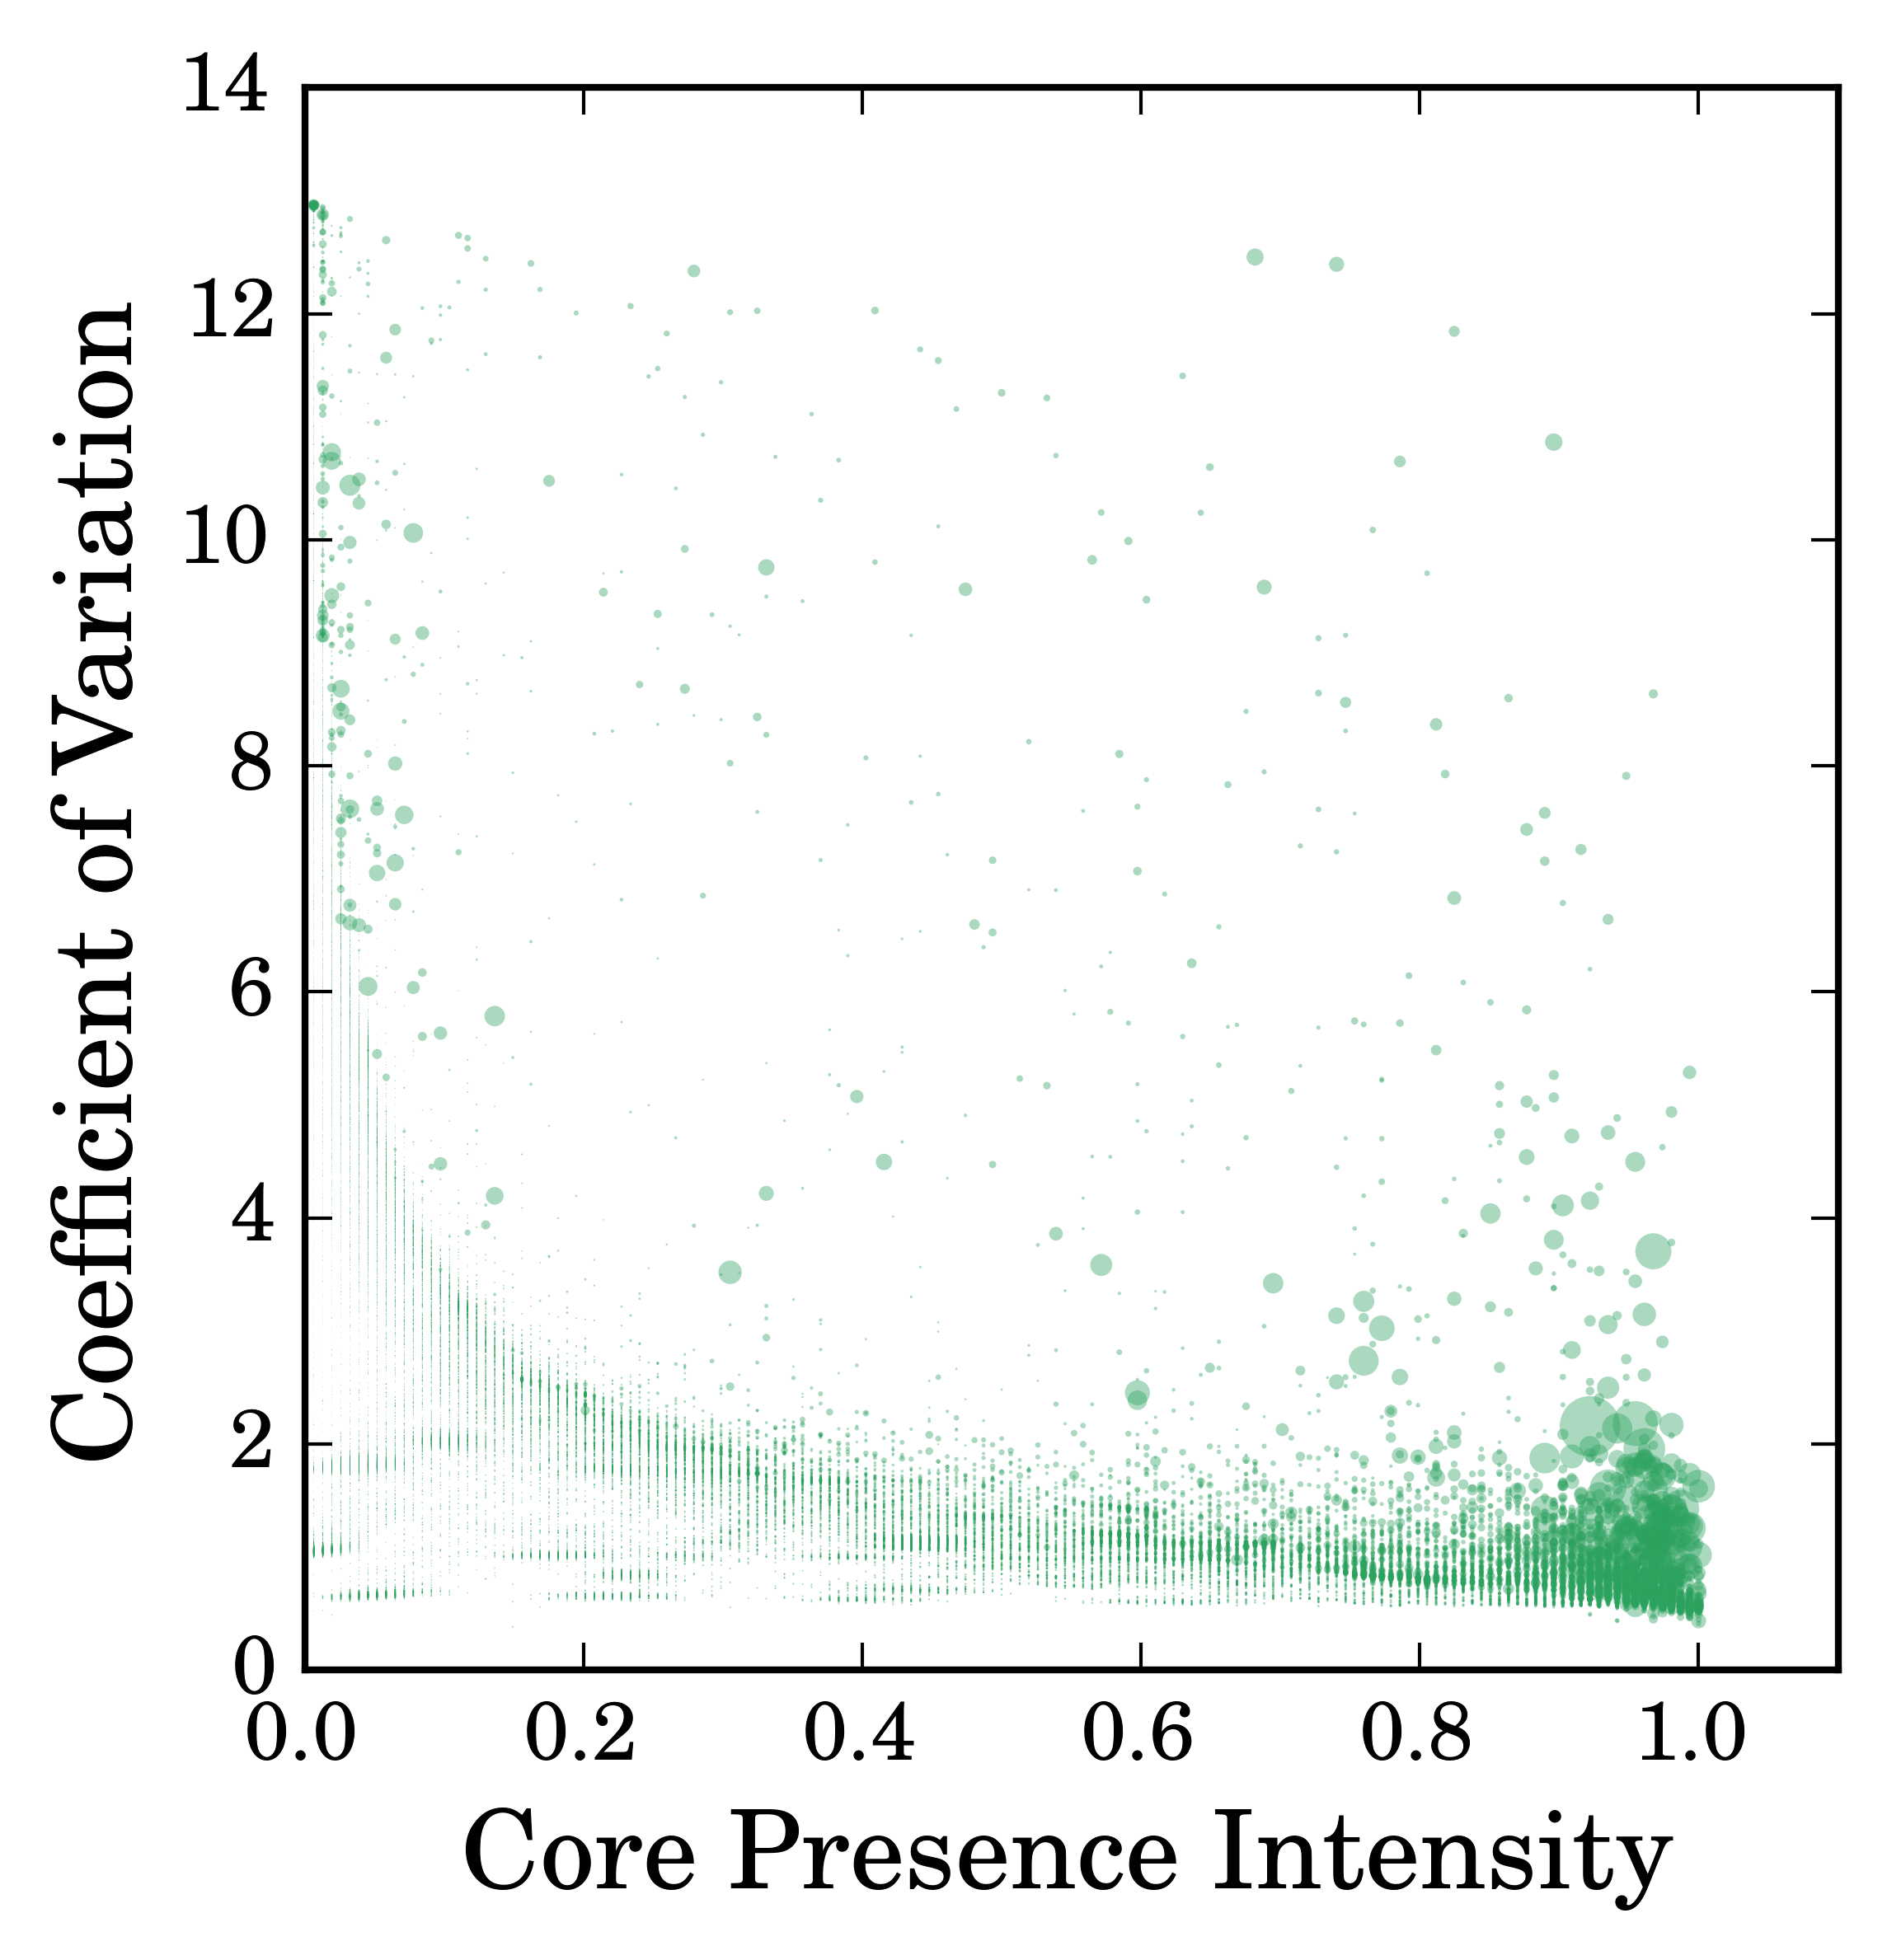
\includegraphics[width=\textwidth]{gfx/chap2/corre_cv_cp_se.png}
                \caption{SE, 86014 prefixes}
                \label{fig:cv_cp_se}
        \end{subfigure}
        \begin{subfigure}[b]{0.49\textwidth}
                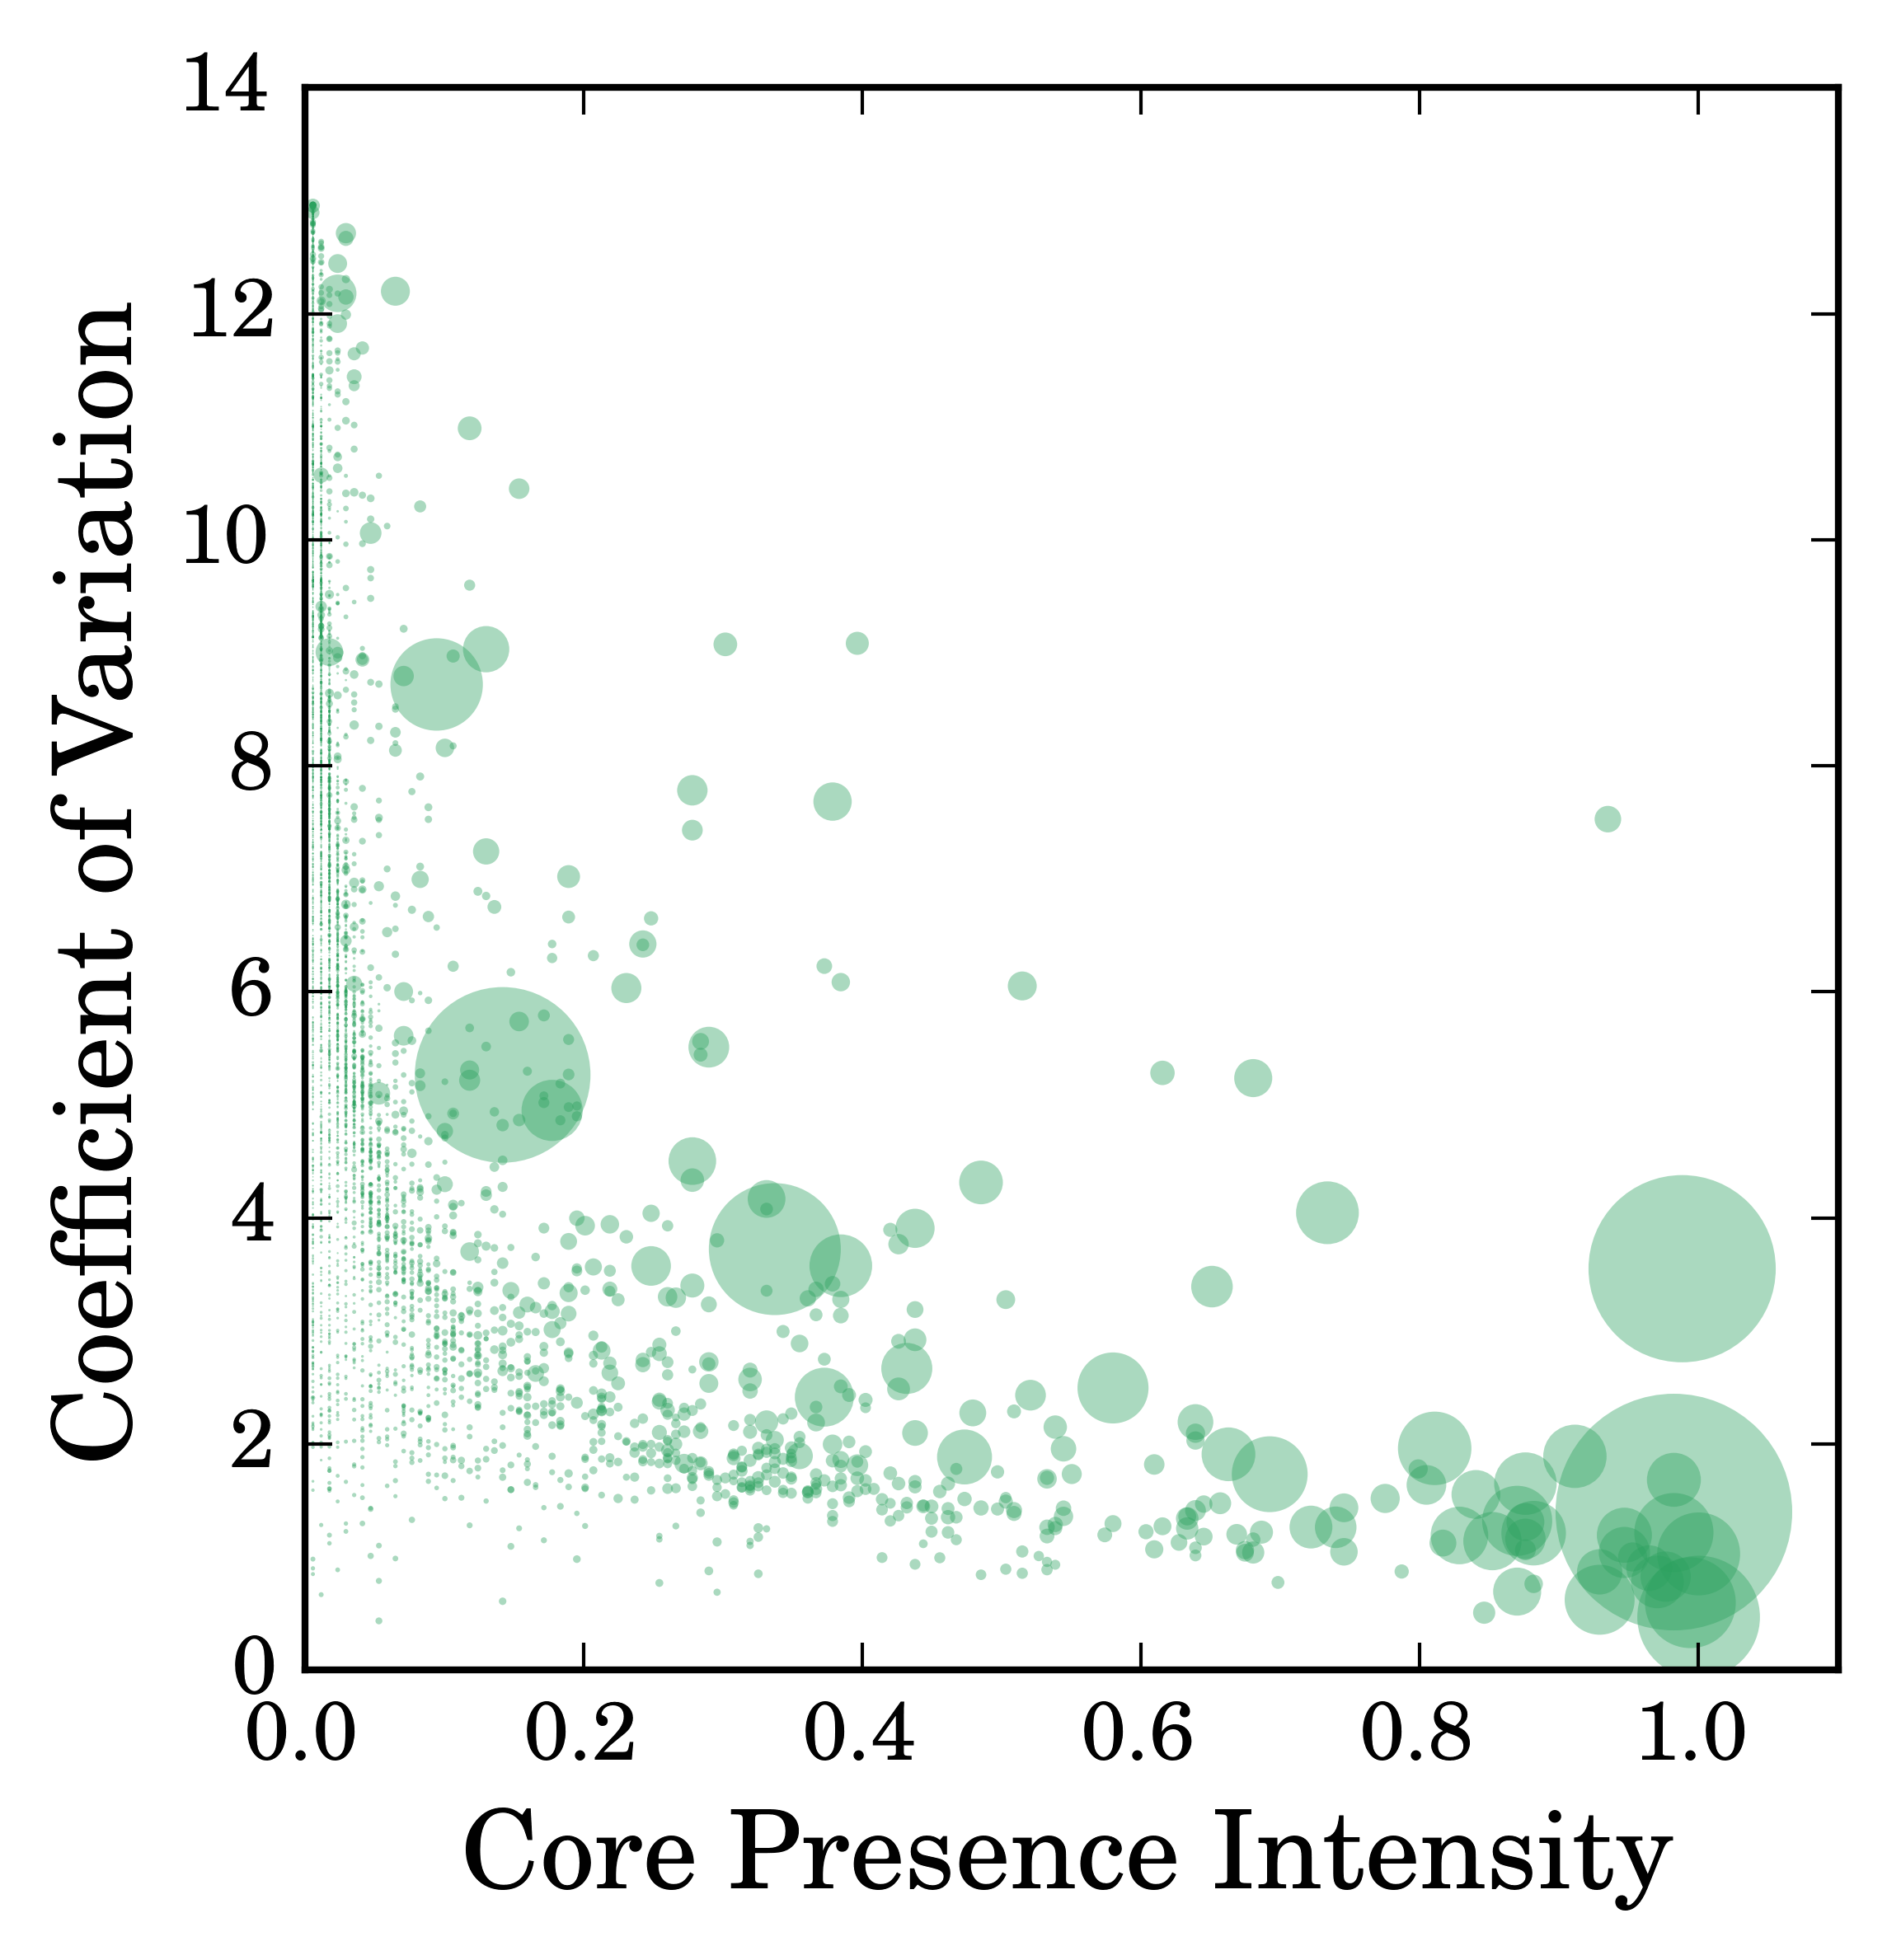
\includegraphics[width=\textwidth]{gfx/chap2/corre_cv_cp_sf.png}
                \caption{SF, 26907 prefixes}
                \label{fig:cv_cp_sf}
        \end{subfigure}
\caption{Relation between $I_{cp}$ over one week and $c_v$ of hour volume over the week from June 1st, 2015. Each circle stands for a prefix. Number of active prefixes plotted is each sub-graph throughout the week is also given. Circle size is proportional to the week volume fraction of the prefix the circle represents and is of the same scale for all networks.}
\label{fig:cv_cp}
\end{figure}
\begin{figure}\ContinuedFloat
	\centering
        \begin{subfigure}[b]{0.49\textwidth}
                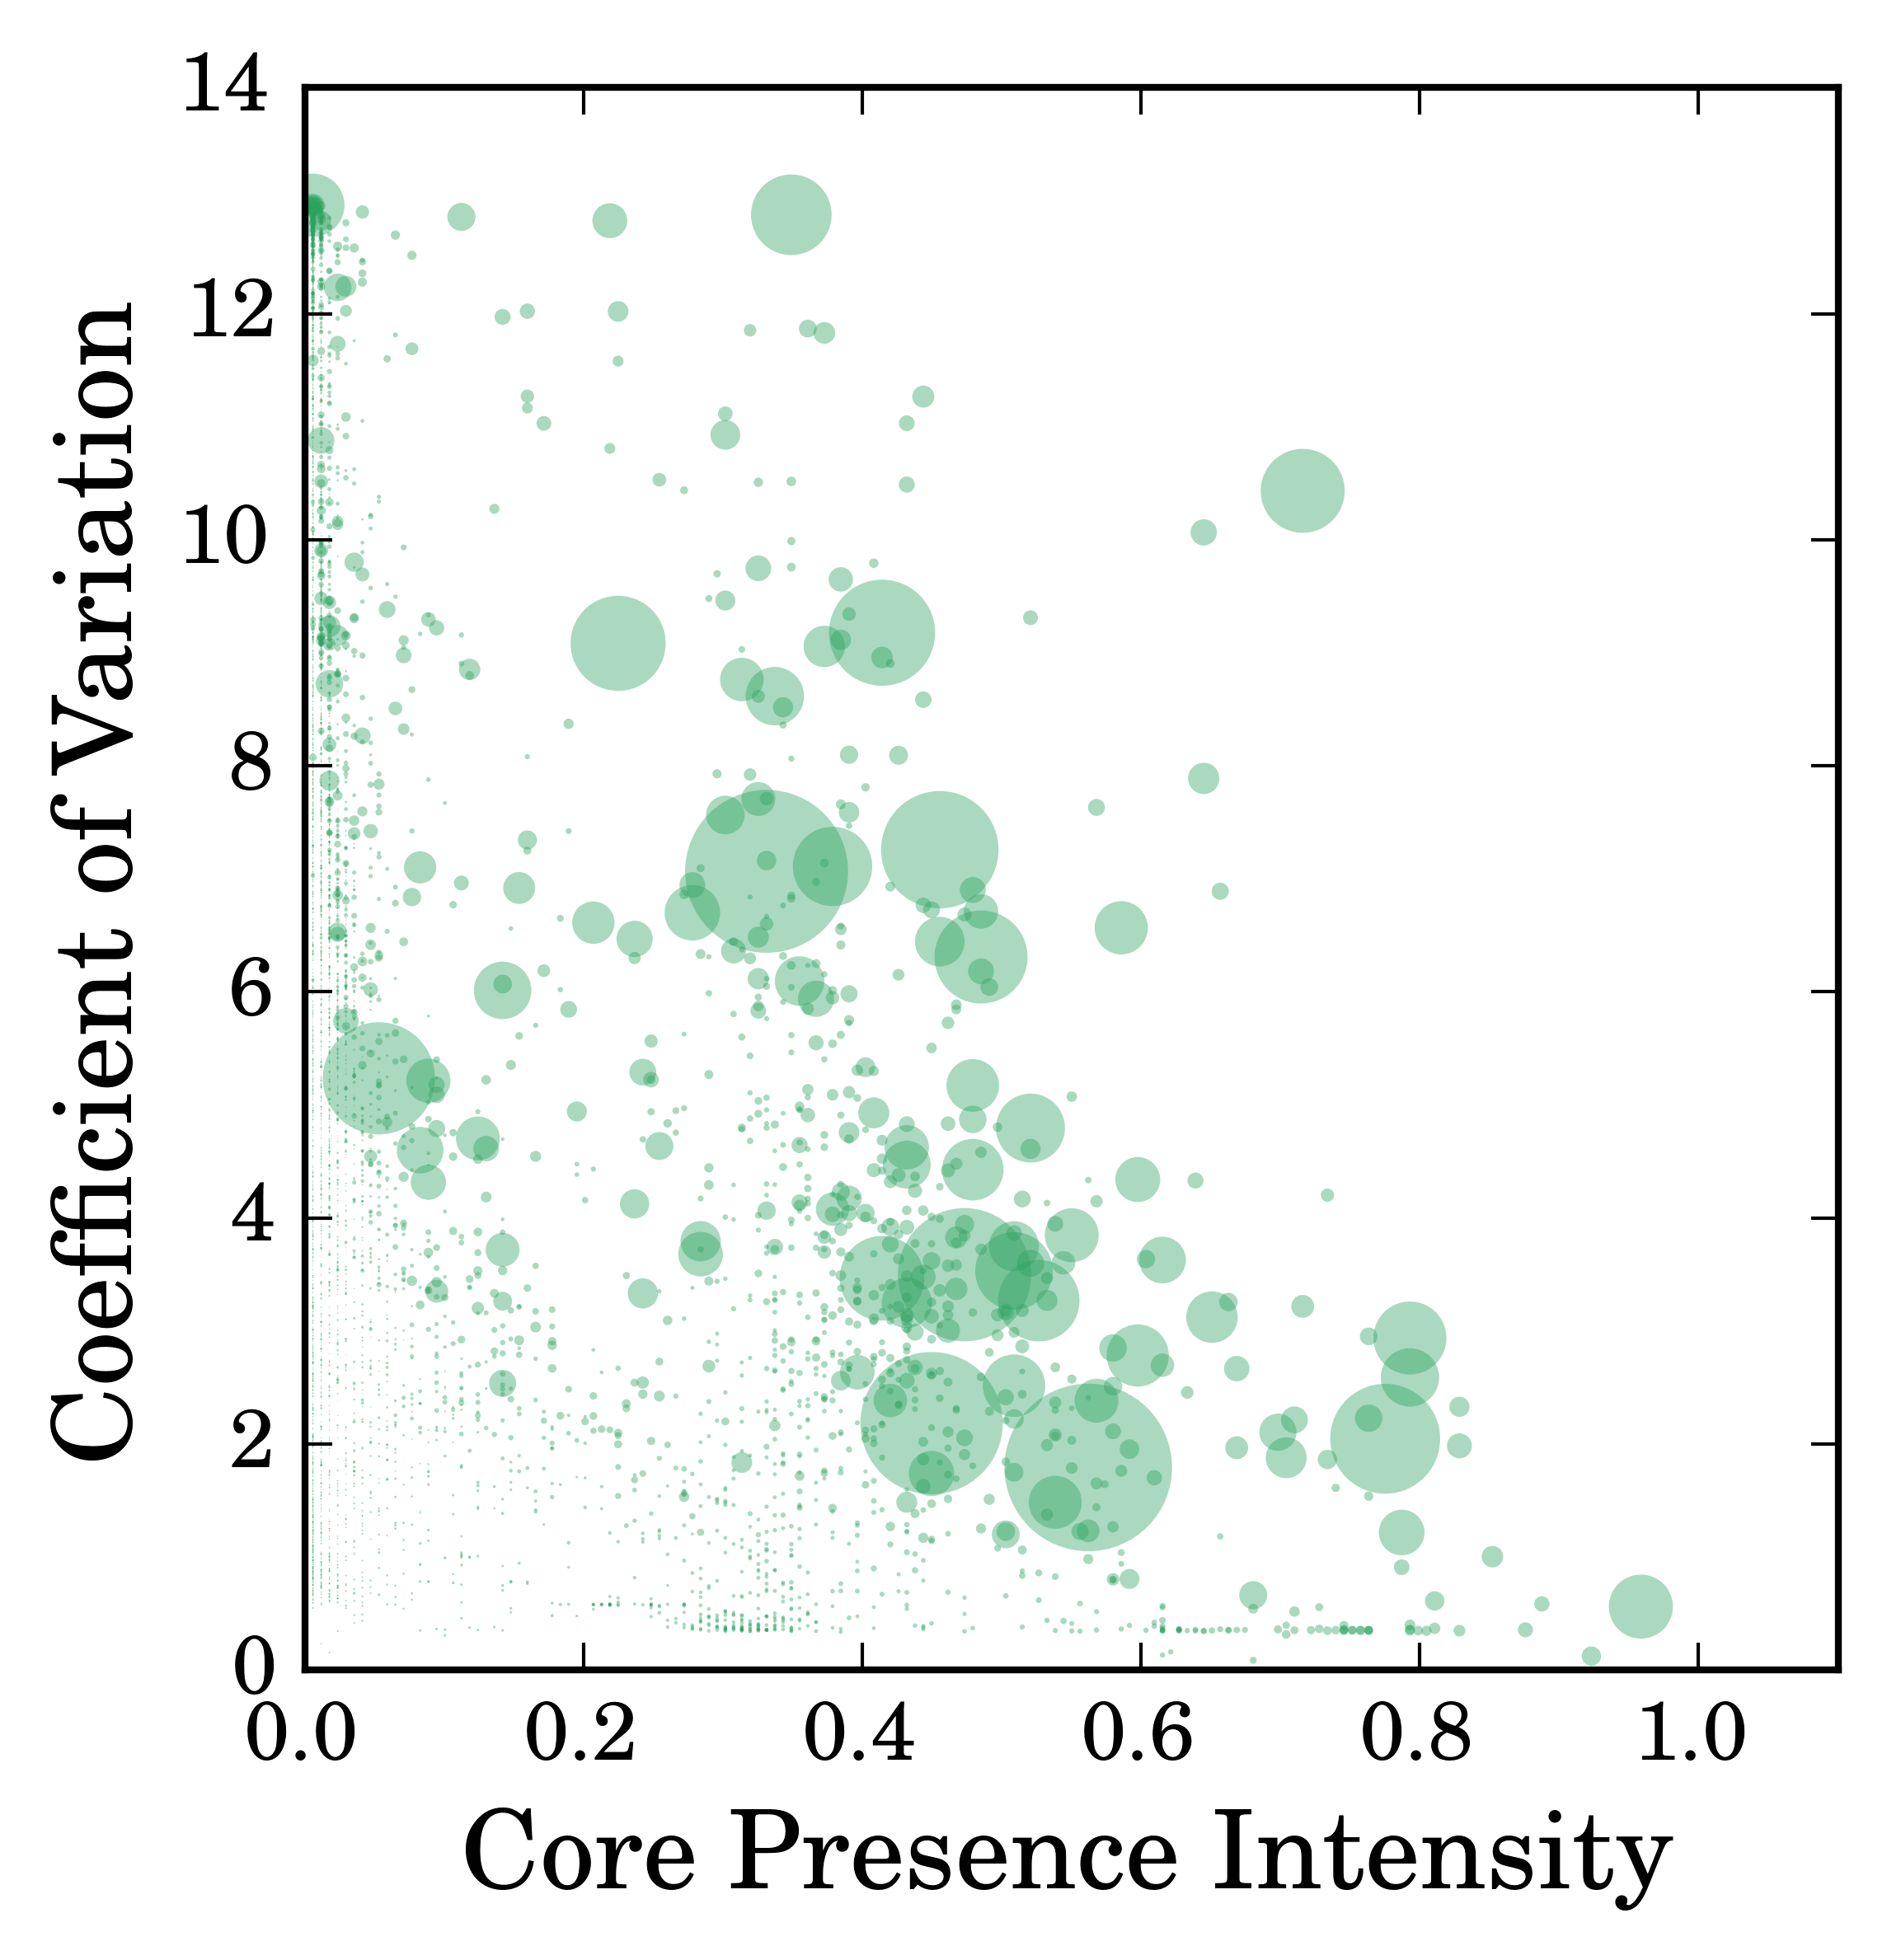
\includegraphics[width=\textwidth]{gfx/chap2/corre_cv_cp_sg.png}
                \caption{SG, 104425 prefixes}
                \label{fig:cv_cp_sg}
        \end{subfigure}
        \begin{subfigure}[b]{0.49\textwidth}
                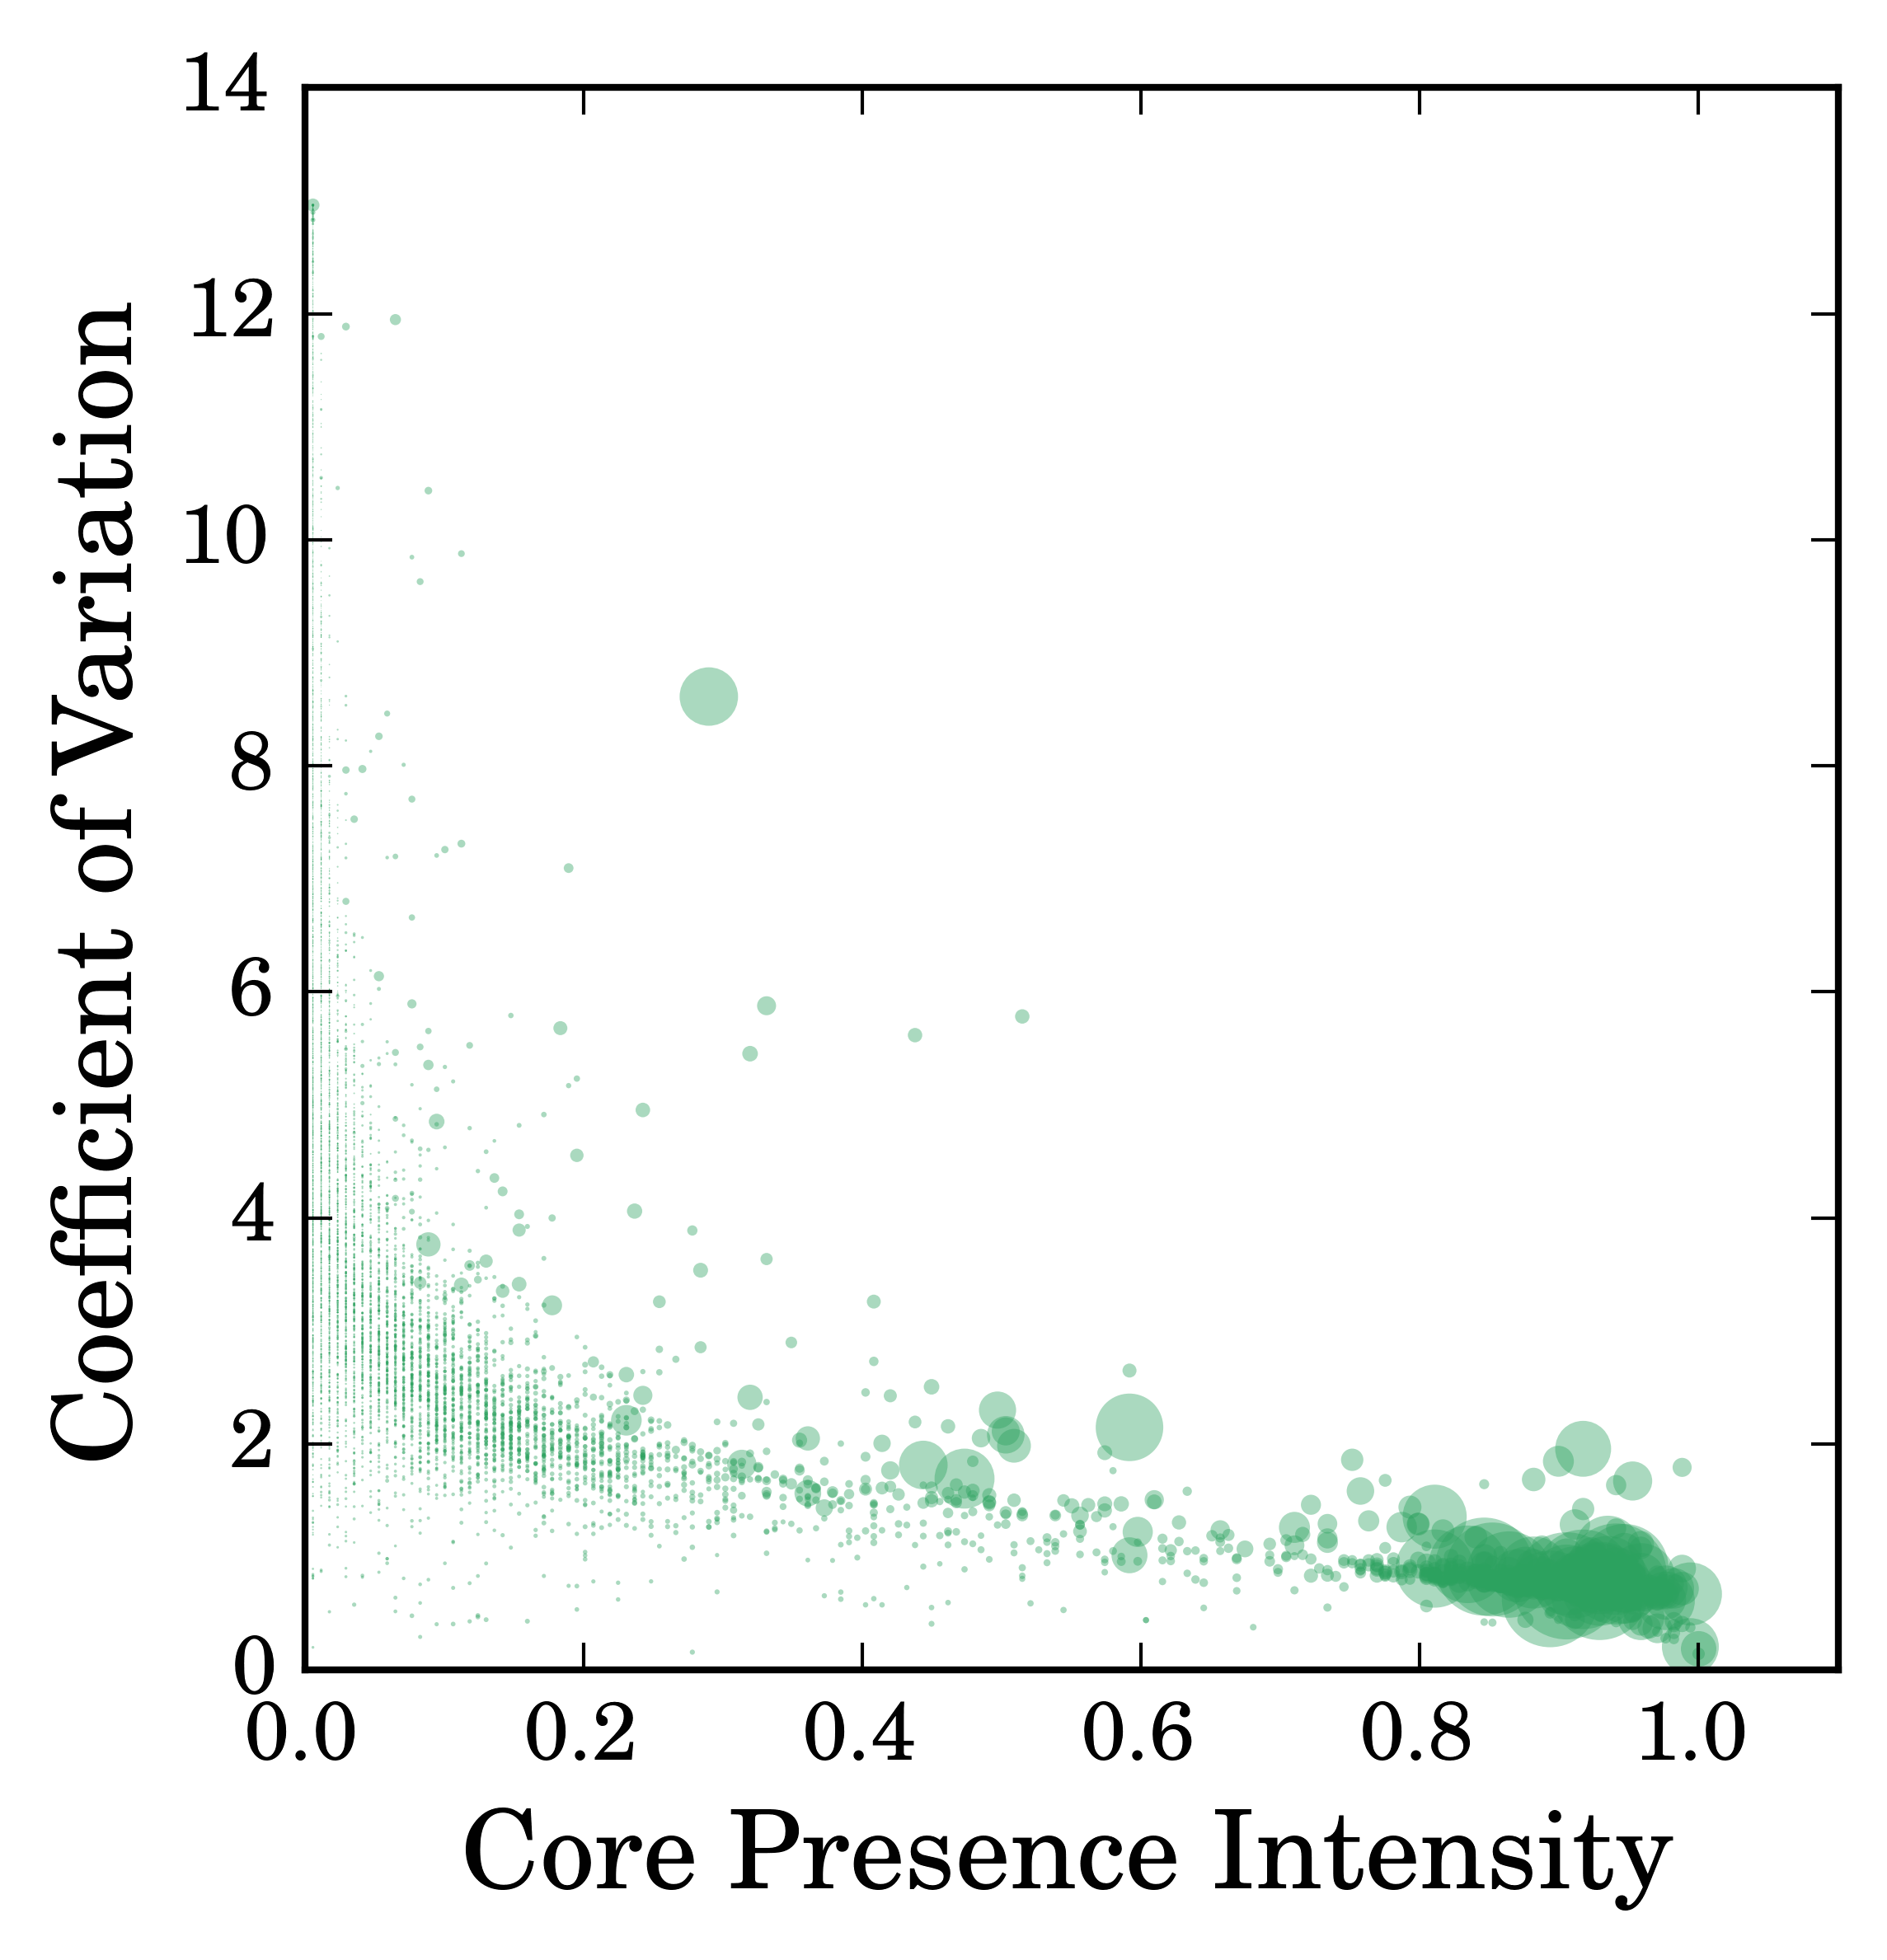
\includegraphics[width=\textwidth]{gfx/chap2/corre_cv_cp_sh.png}
                \caption{SH, 52061 prefixes}
                \label{fig:cv_cp_sh}
        \end{subfigure}
        \begin{subfigure}[b]{0.49\textwidth}
                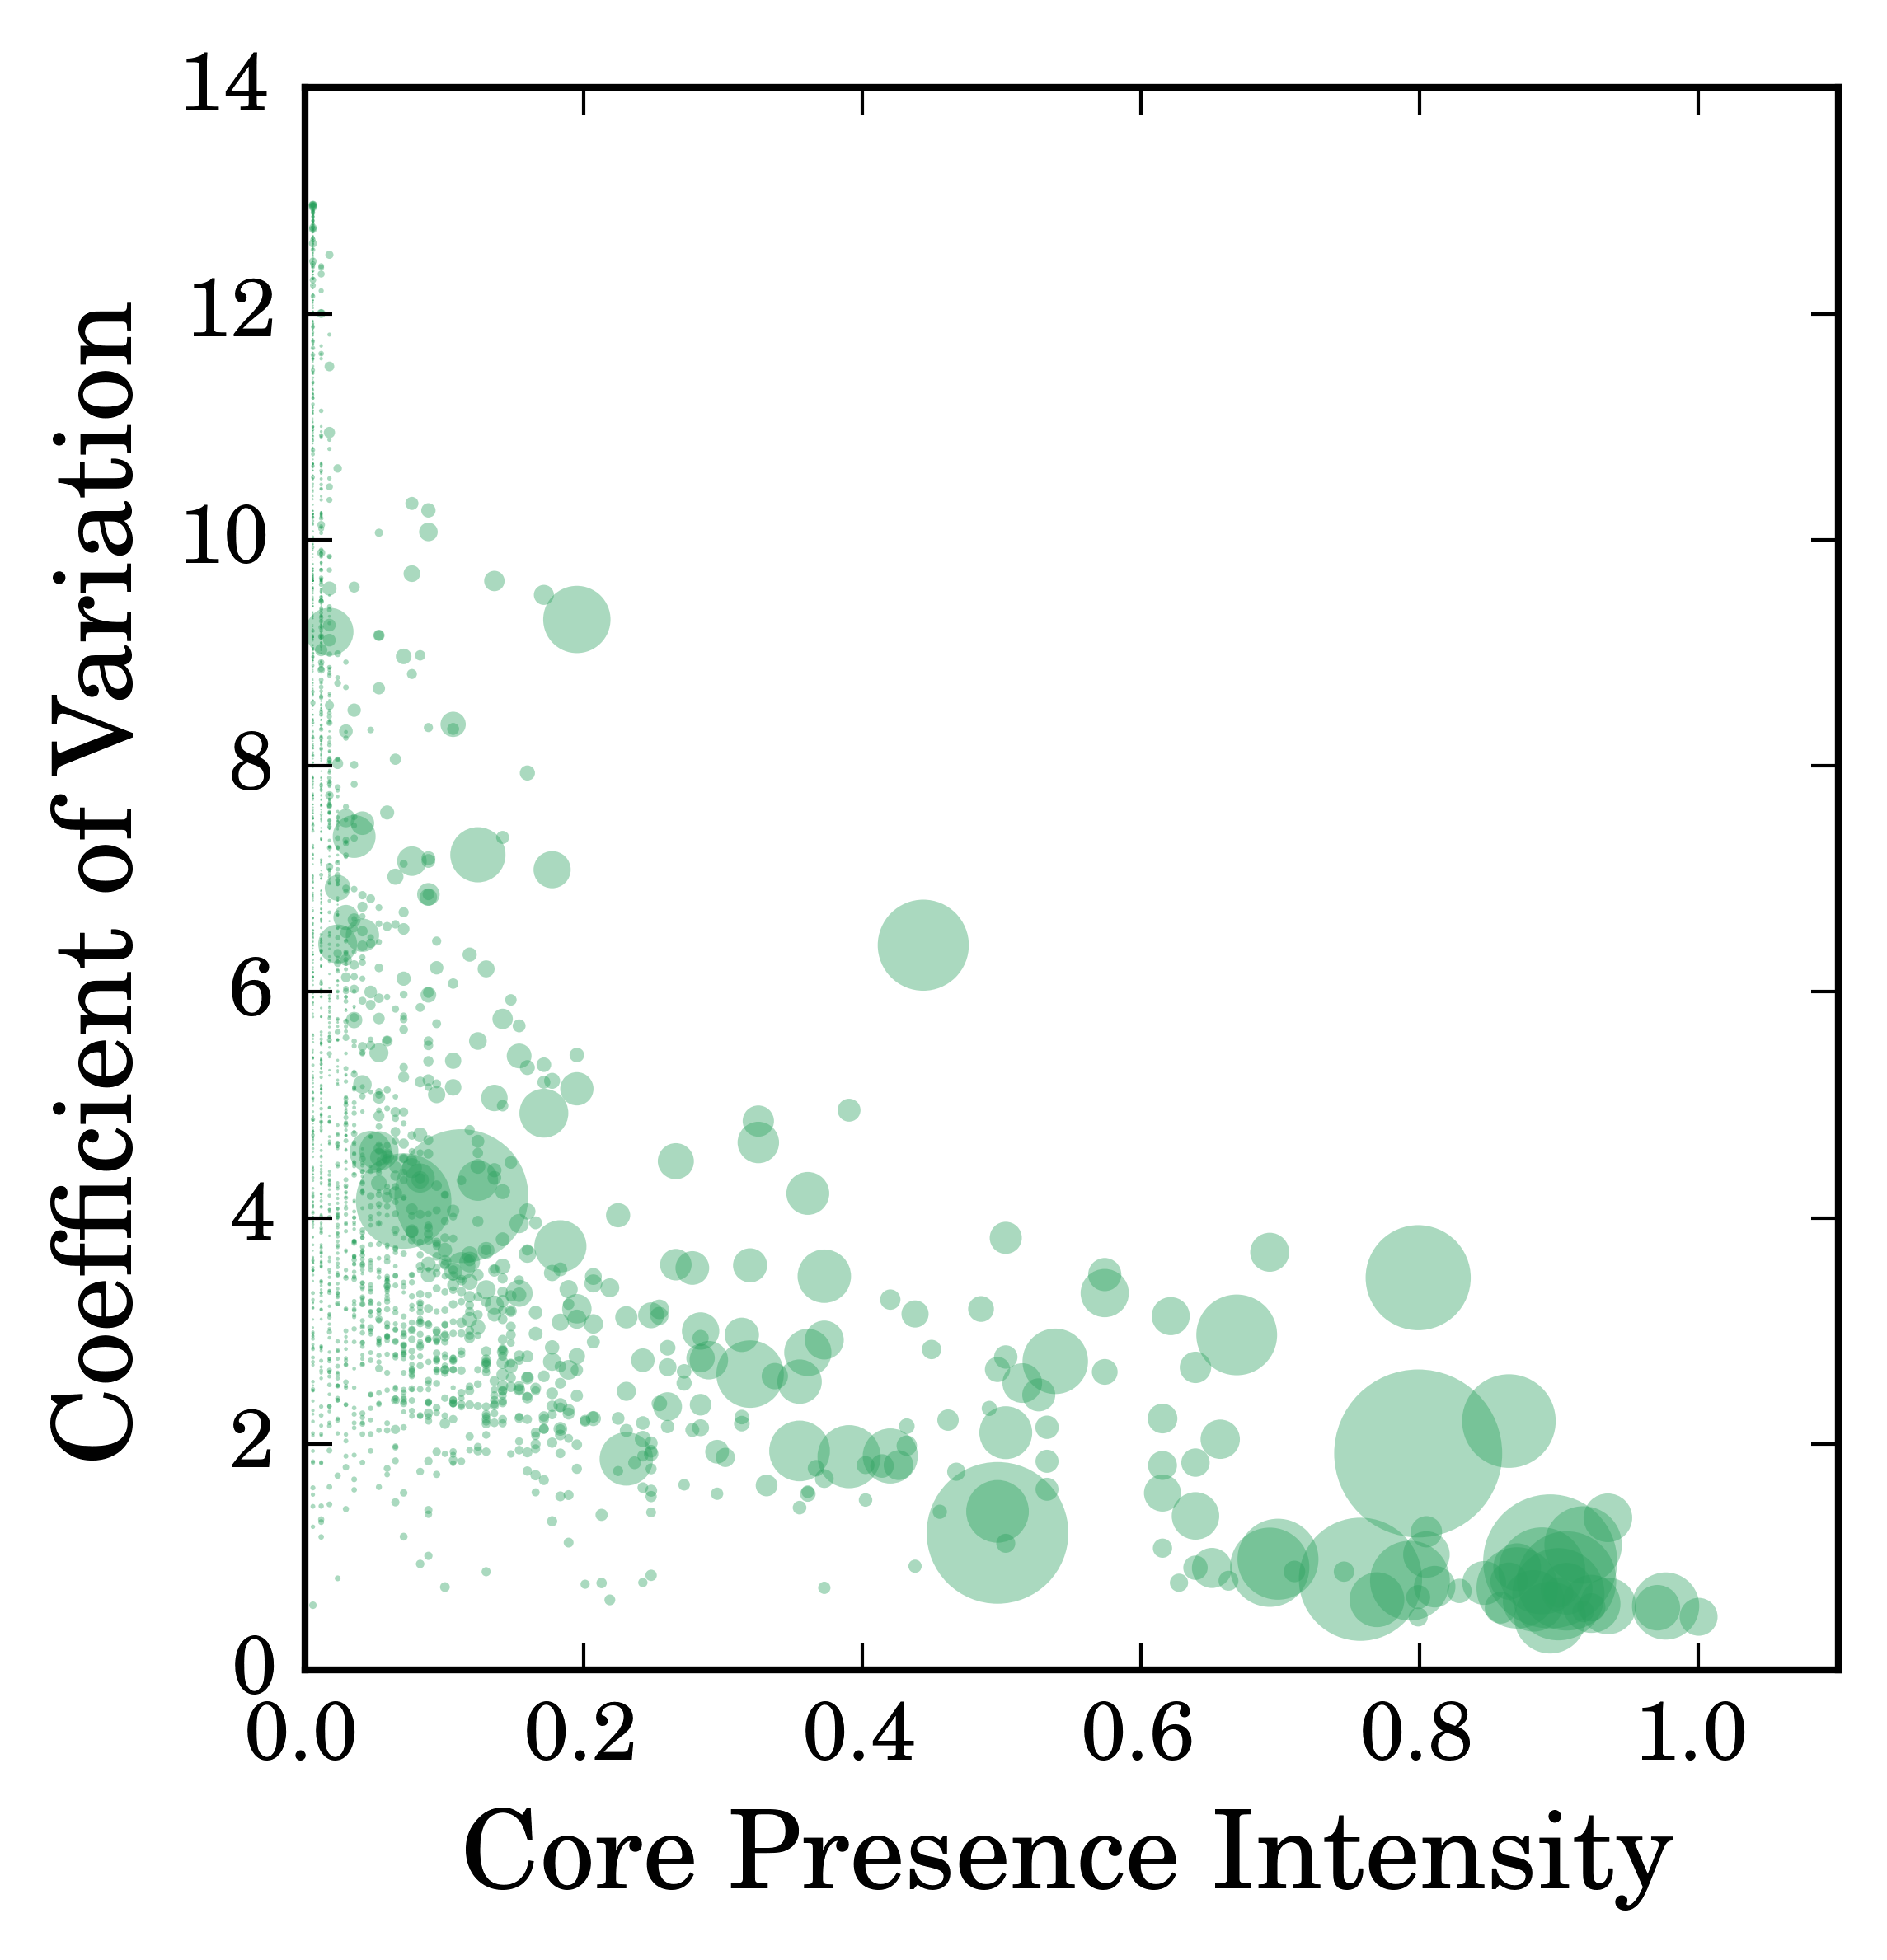
\includegraphics[width=\textwidth]{gfx/chap2/corre_cv_cp_si.png}
                \caption{SI, 14189 prefixes}
                \label{fig:cv_cp_si}
        \end{subfigure}
\caption{(cont.) Relation between $I_{cp}$ over one week and $c_v$ of hour volume over the week from June 1st, 2015.}
\label{fig:cv_cp_cont}
\end{figure}

It is interesting to study the correlation between these two metrics: $c_v$ %of hour volume throughout the week 
and $I_{cp}$ in Fig.~\ref{fig:cv_cp}, where each circle represents a prefix and its radius is proportional to the prefix's week volume share.
The biggest circles mostly concentrate in the lower right corner of each sub-graph, which corresponds to the remarks made previously.
However, some exceptions exist, especially on SC (but also SF, SG and SI), where we observe circles of big sizes having low $I_{cp}$ and relatively high $c_v$.
These prefixes bring significant traffic volume share within a short duration, which makes predictive prefix selection difficult. 
Finally, it's not a surprise to see that the $c_v$ of prefixes with big week volume is, to a certain extent, inversely correlated to their $I_{cp}$.
%That is, when a prefix is associated with larger week traffic volume, chances are it has smaller variation in hour volumes and presents more often in the \textit{core} set.

\subsubsection{A view at hour interval}
\begin{figure}
\centering
        \begin{subfigure}[b]{0.85\textwidth}
                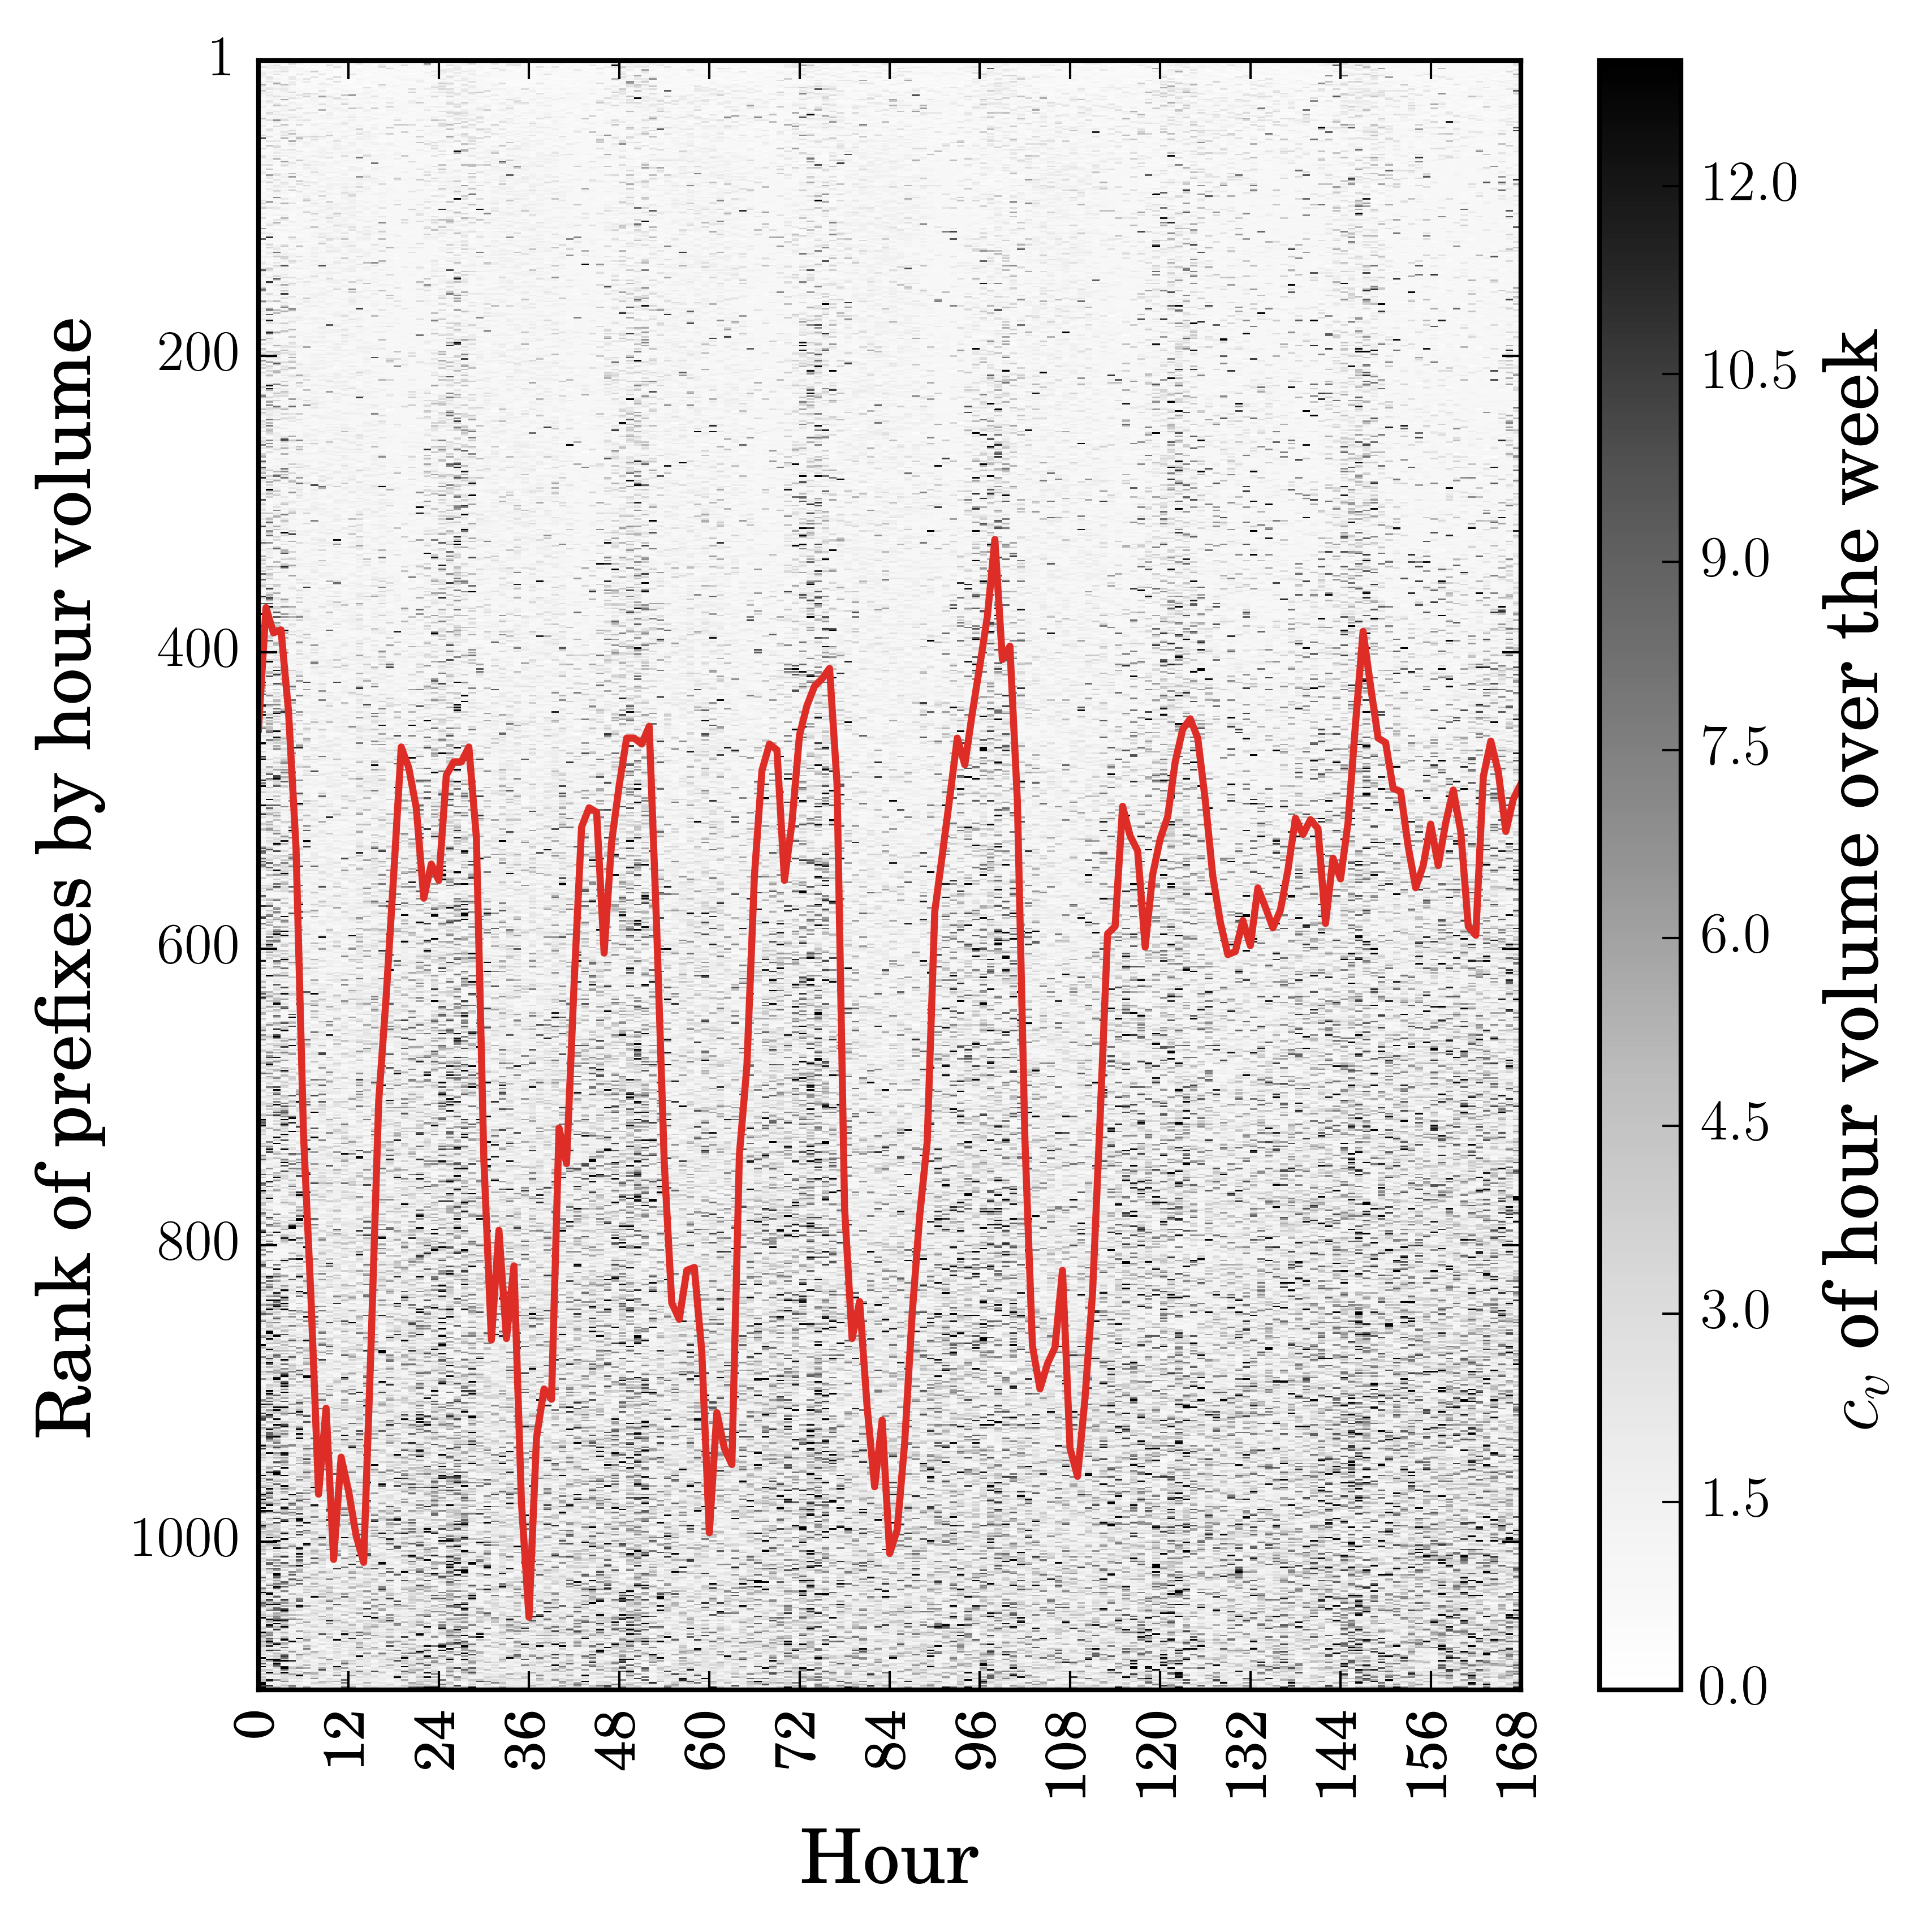
\includegraphics[width=\textwidth]{gfx/chap2/cv_mat_sa.png}
                \caption{$c_v$}
                \label{fig:cv_mat_sa}
        \end{subfigure}
        \begin{subfigure}[b]{0.85\textwidth}
                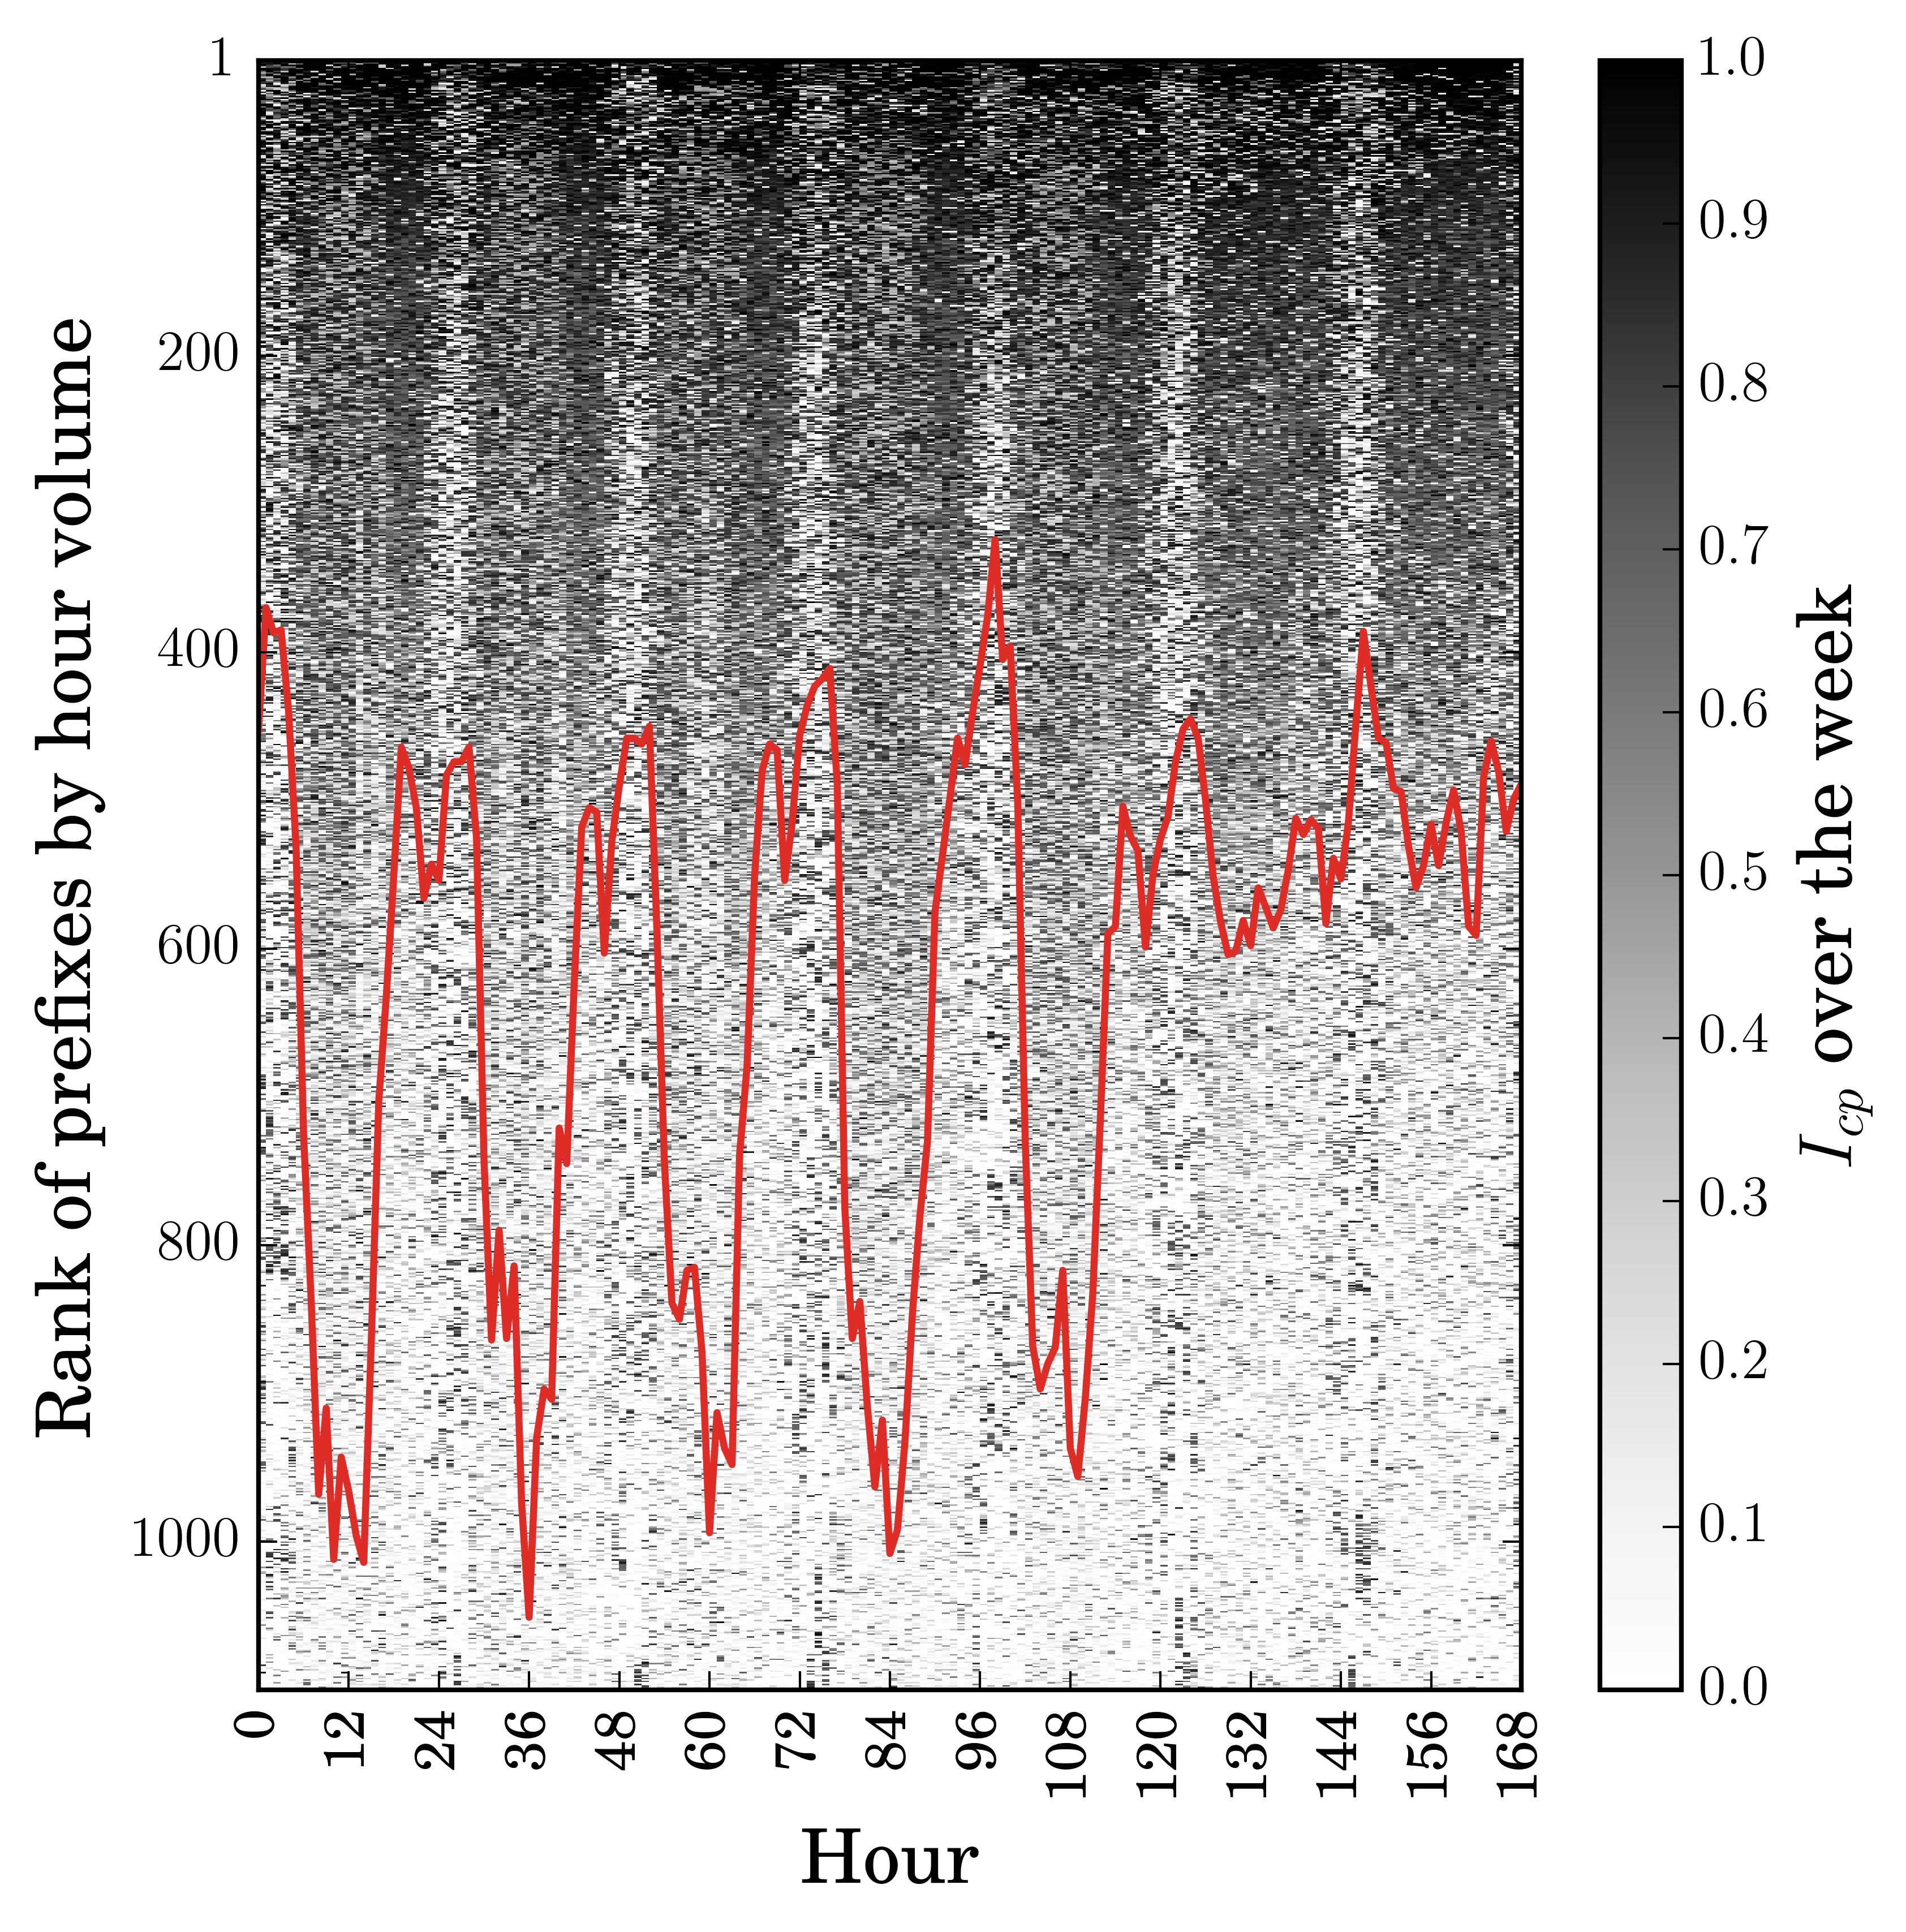
\includegraphics[width=\textwidth]{gfx/chap2/cp_mat_sa.png}
                \caption{$I_{cp}$}
                \label{fig:cp_mat_sa}
        \end{subfigure}
\caption{$c_v$ and $I_{cp}$ over one week for top ranked prefixes at each hour on SA. Prefixes are ranked by their hour volume along the column (big prefixes at the top). Their $c_v$ or $I_{cp}$ over the week are represented by the grey scale. Red line indicates the number of prefixes in \textit{core} prefix set each hour.}
\label{fig:cv_cp_mat}
\end{figure}

\marginpar{traffic dynamism at finer time resolution}
The above analyses at week scale conclude that most prefixes associated with a big volume over a long term tend to be stable in hour volume variation and present often in \textit{core}, though a few exceptions exist.
Here, we explore the prefix volume dynamism at hour resolution by visualizing them in Fig.~\ref{fig:cv_cp_mat}, where each column corresponds to top prefixes ranked by their hour volume with large volume prefixes at the top and small ones at the bottom. A grey scale tile is used to portrait the $c_v$ or $I_{cp}$ over the week for each prefix. Prefixes above the red line are those composing \textit{core} at each hour.
Only graphs for SA are shown for the patterns demonstrated are most informative and less noisy due to less bursty traffic.

\marginpar{observations from $c_v$ graph}
In Fig.~\ref{fig:cv_mat_sa} the graph for $c_v$, area above the red line has observably lighter value than the lower part. 
This implies that in each hour, prefixes in the \textit{core} have more stable hour volume over a long term, i.e. closer to its mean value,  than those outsiders with little volume significance.
Moreover, the figure demonstrates as well a time-of-day pattern. 
During late night and early morning, prefixes in the \textit{core} have deeper color, thus more volatile, than those in the day time, which indicates that important prefixes composition are not quite the same during these two periods.
The above described phenomenon are sometimes a little bit more difficult to be perceived on other networks with more bursty traffic. 
Nonetheless, the color value for \textit{core} area is not visibly darker.
It means the hourly volume time series for large prefixes are not obviously less stable.
We should all the same be able to pick them out using their mean value.
The lack of clear diurnal pattern for some networks is possibly related to their business types and client populations they serve, which is out of the scope of this work.

\marginpar{observations from $I_{cp}$ graph}
When it comes to $I_{cp}$, it is true for all networks that top ranked prefixes each hour are more likely to frequently appear in the \textit{core} prefix set, which leads to deeper color at the top.
However, we can witness light spots each hour in the upper part of the graph, which corresponds to bursty traffic.
Further, the color difference across the red line is not obvious.
This indicates $I_{cp}$ alone is not informative enough to tell whether a prefix brings a big amount of traffic at a certain hour, though for long term it demonstrate strong correlation with volume importance as seen in Fig.~\ref{fig:cpi}.
Time-of-day pattern can also be clearly observed. It confirms again that prefixes active over night are different from those during the day time.


\subsection{Quantitative index of traffic burstiness}
Previous explorations has shown that the predictability of traffic volume from a client network is related to its traffic burstiness.
In order to describe this feature in a quantitative manner, we define the index $\beta(P)_h$, for a prefix $P$ at certain hour $h$ as:
\begin{equation*}
\beta(P)_i = \begin{dcases*}
         -\log(I_{cp}(P)) \times vp(P)_i & if $I_{cp}(P) > 0$\\
        0 & if $I_{cp}(P) = 0$,
        \end{dcases*}
\label{eq:beta}
\end{equation*}
where $vp(P)_h$ is the hour volume percentage (among all active prefixes) of prefix $P$ at hour $h$.
The logarithmic term applied on $I_{cp}$ aims at amplifying the volume contribution of prefixes with rare \textit{core} presence, and attenuating the influence of prefixes being intensively in the \textit{core}.
A large $\beta$ value indicates that it is hard to predict the volume associated with this prefix while representing a significant hour volume.

In order to estimate the overall burstiness of all prefixes at hour $h$ for a client network, we sum up the $\beta(P)_h$ for each $P$ inside the \textit{core} of that hour: more formally, 
%Wenqin: notation for $\beta(P)_i$ is not right
\begin{equation*}
BI_h = \sum_{P \in \textit{core}_h} \beta(P)_h.
\label{eq:bi}
\end{equation*}
%Wenqin: notation for $\beta(P)_i$ is not right
For all the networks, we estimate their traffic burstiness with the mean and maximum value of $BI$ series over the week. The results are given in Table~\ref{tab:bi}. The maximum $\beta$, contribution from a single prefix, throughout the week is also given.

\begin{table}[!htb]
\centering
\begin{tabular}{cccc}\toprule
\textbf{Network} & \textbf{Mean $BI$} & \textbf{Max $BI$} & \textbf{Max $\beta$}\\
\midrule
SA & 14.61 & 37.79  &  7.44\\
SB & 31.09 & 46.85  &  4.08\\
SC & 40.57 & 145.07 &  145.05\\
SD & 42.14 & 69.34  &  18.10\\
SE & 20.91 & 44.30  &  20.17\\
SF & 44.10 & 98.69  &  78.77\\
SG & 51.21 & 125.41 &  102.05\\
SH & 15.91 & 35.06  &  16.29\\
SI & 38.59 & 85.47  &  56.56\\
\bottomrule
\end{tabular}
\caption{Traffic burstiness.}
\label{tab:bi}
\end{table}

Mean $BI$ over the week measures the general burstiness of traffic, while maximum $BI$ describes the degree of burstiness in worst cases.
In accordance to the observation made from Fig.~\ref{fig:cv_cp}, there are big volume prefixes with fairly low $I_{cp}$ on SC, SF, SG and SI, whence the much bigger maximum $\beta$ value.
What is less evident in Fig.~\ref{fig:cv_cp} is that SD suffers actually a lot from bursty traffic, even more than SC in general.
For the rest networks, i.e. SA, SB, SE and SH, their mean $BI$ over the week is around 30 or lower. Their corresponding sub-graphs in Fig.~\ref{fig:cv_cp} manifest as well much less big circles on the left side where $I_{cp}$ is low.
More specifically SB suffers more from bursty traffic than SA, therefore bigger value in both maximum and mean $BI$ over the week, which is as well not easy to tell directly from Fig.~\ref{fig:cv_cp}.
%which is in accordance with the observation that the tone of \textit{core} area of SB is lighter than that of SA in Fig~\ref{fig:cp_mat}.
Still, the maximum $\beta$ on SA is larger than that on SB, which is due to the fact that traffic on SB is more evenly distributed among active prefixes (see Fig.~\ref{fig:traffic_dis_site}), and the faction of traffic associated to each prefix is generally smaller.
In short, we found this simple metric capable of describing the traffic burstiness of the networks studied.


\section{Predictive prefix selection}
\label{sec:sele}

\subsection{Candidate prediction metrics}

\marginpar{prediction metrics inspired by traffic temporal dynamism studies}
Based on the previous observations, several approaches naturally emerges for the prediction of traffic volume ``importance'' of a prefix.
\paragraph*{Mean Volume}
With this metric, we predict that at hour $h+1$, the volume importance of prefix $P$ is indicated by it's mean hourly volume over the last $L$ hours, $MV(P,L)_{h+1} = 1/L \times \sum_{i = h-L+1}^{h} v(P)_i$.
It is based on the observations from Fig.~\ref{fig:cv}, that top prefixes ranked over the week tend to have smaller hourly volume variation around their mean volume.

\paragraph*{Core Presence Intensity}
The prediction could use $I_{cp}(P,L)_{h+1} = 1/L \times \sum_{i = h-L+1}^{h} cp(P)_i$, i.e. the \textit{core} presence intensity of the prefix over the last $L$ hours. It derives from the observation made from Fig.~\ref{fig:cpi}, that top ranked prefixes by their week volume are more likely to have intense \textit{core} presence.

\paragraph*{Core Volume}
Finally, the prediction could be based on $CV(P,L)_{h+1} = 1/L \times \sum_{i = h-L+1}^{h} cp(P)_i \times v(P)_i$,  a combination of both $MV$ and $I_{cp}$.
$CV$ has the potential to be more resource thrifty compared to $MV$, as it is calculated only for those prefixes ever appeared in the \textit{core} over the last $L$ hours --- while $MV$ is computed for all active prefixes. From our observations, the \textit{core} size actually represents $5\%$ to $50\%$ of all active prefixes.

\subsection{Grey model as reference method}
\marginpar{computation complexity}
In previous work by Zhange et al.\ \cite{Zhang2012} on FIB caching, a grey differential model $GM(1,1)$ \cite{Julong1989} is employed to predict which BGP prefixes will represent the  biggest packet counts. 
It is by far more computationally efficient ($O(L)$), compared to \ac{TSF} methos such as \ac{ANN} ($O(L*M)$) and \ac{ARIMA} ($O(L^2)$), where L is the length of time series, M is the number of hidden nodes in the neural network.
For the sake of comparison, we implemented the $GM(1,1)$ model in our work. 

A brief introduction to this model and how we apply it in our context is given below. Mathematical details of this model can be find in the work by Deng \cite{Julong1989}.
$GM(1,1)$ predicts the cumulative hour volume $v^1$ instead of hour volume directly:
\begin{equation*}
v^1(P,L)_{i} = \displaystyle \sum_{j=i-L+1}^{i} v(P)_j,
\end{equation*}
where $v^1(P,L)_{i}$ is the cumulative hour volume of prefix $P$ over last $L$ hours at hour $i$. The purpose is to derive $v(P)_{i+1}$, i.e. the volume in the following hour, from estimations of cumulative volumes of hour $i+1$ and $i$:
\begin{equation*}
\hat{v}(P)_{i+1} = \hat{v}^1(P,L)_{i+1} - \hat{v}^1(P,L)_{i},
\end{equation*}
where $\hat v$ and $\hat v ^1$ are all estimation values given by the model.
$GM(1,1)$ predicts that the cumulative hour volume at hour $i+1$ equals:
\begin{equation*}
\hat v ^1 (P,L)_{i+1} = (v(P)_{i-L+1} - \frac{b}{a}) e^{-aL} + \frac{b}{a},
\end{equation*}
where $a$ and $b$ are parameters that can be estimated with least square method (symbol with hat are all estimations).
\begin{equation*}
\mathbf{\hat a} = \begin{bmatrix}
\hat a \\ \hat b
\end{bmatrix} = \mathbf{(B^TB)^{-1}B^T Y},
\end{equation*}
where
\begin{equation*}
\mathbf{B} = \begin{bmatrix}
-0.5(v^1(P,L)_{i-L+2} + v^1(P,L)_{i-L+1}) & 1\\
-0.5(v^1(P,L)_{i-L+3} + v^1(P,L)_{i-L+2}) & 1\\
\cdots & \cdots \\
-0.5(v^1(P,L)_i + v^1(P,L)_{i-1}) & 1
\end{bmatrix},
\end{equation*}
\begin{equation*}
\mathbf{Y} = \begin{bmatrix}
v(P)_{i-L+2}\\
v(P)_{i-L+3}\\
\cdots\\
v(P)_i
\end{bmatrix}.
\end{equation*}

We can see that for each single prefix, two parameters are to be estimated, $a$ and $b$, at each hour based on a new volume series that slides over time. Computationally, estimation with $GM(1,1)$ is much heavier than the three metrics proposed above, the calculation of which is identically to all prefixes without parameters to be customize.

\subsection{Prefix selection evaluation}
\begin{figure}
		\centering
        \begin{subfigure}[b]{0.48\textwidth}
                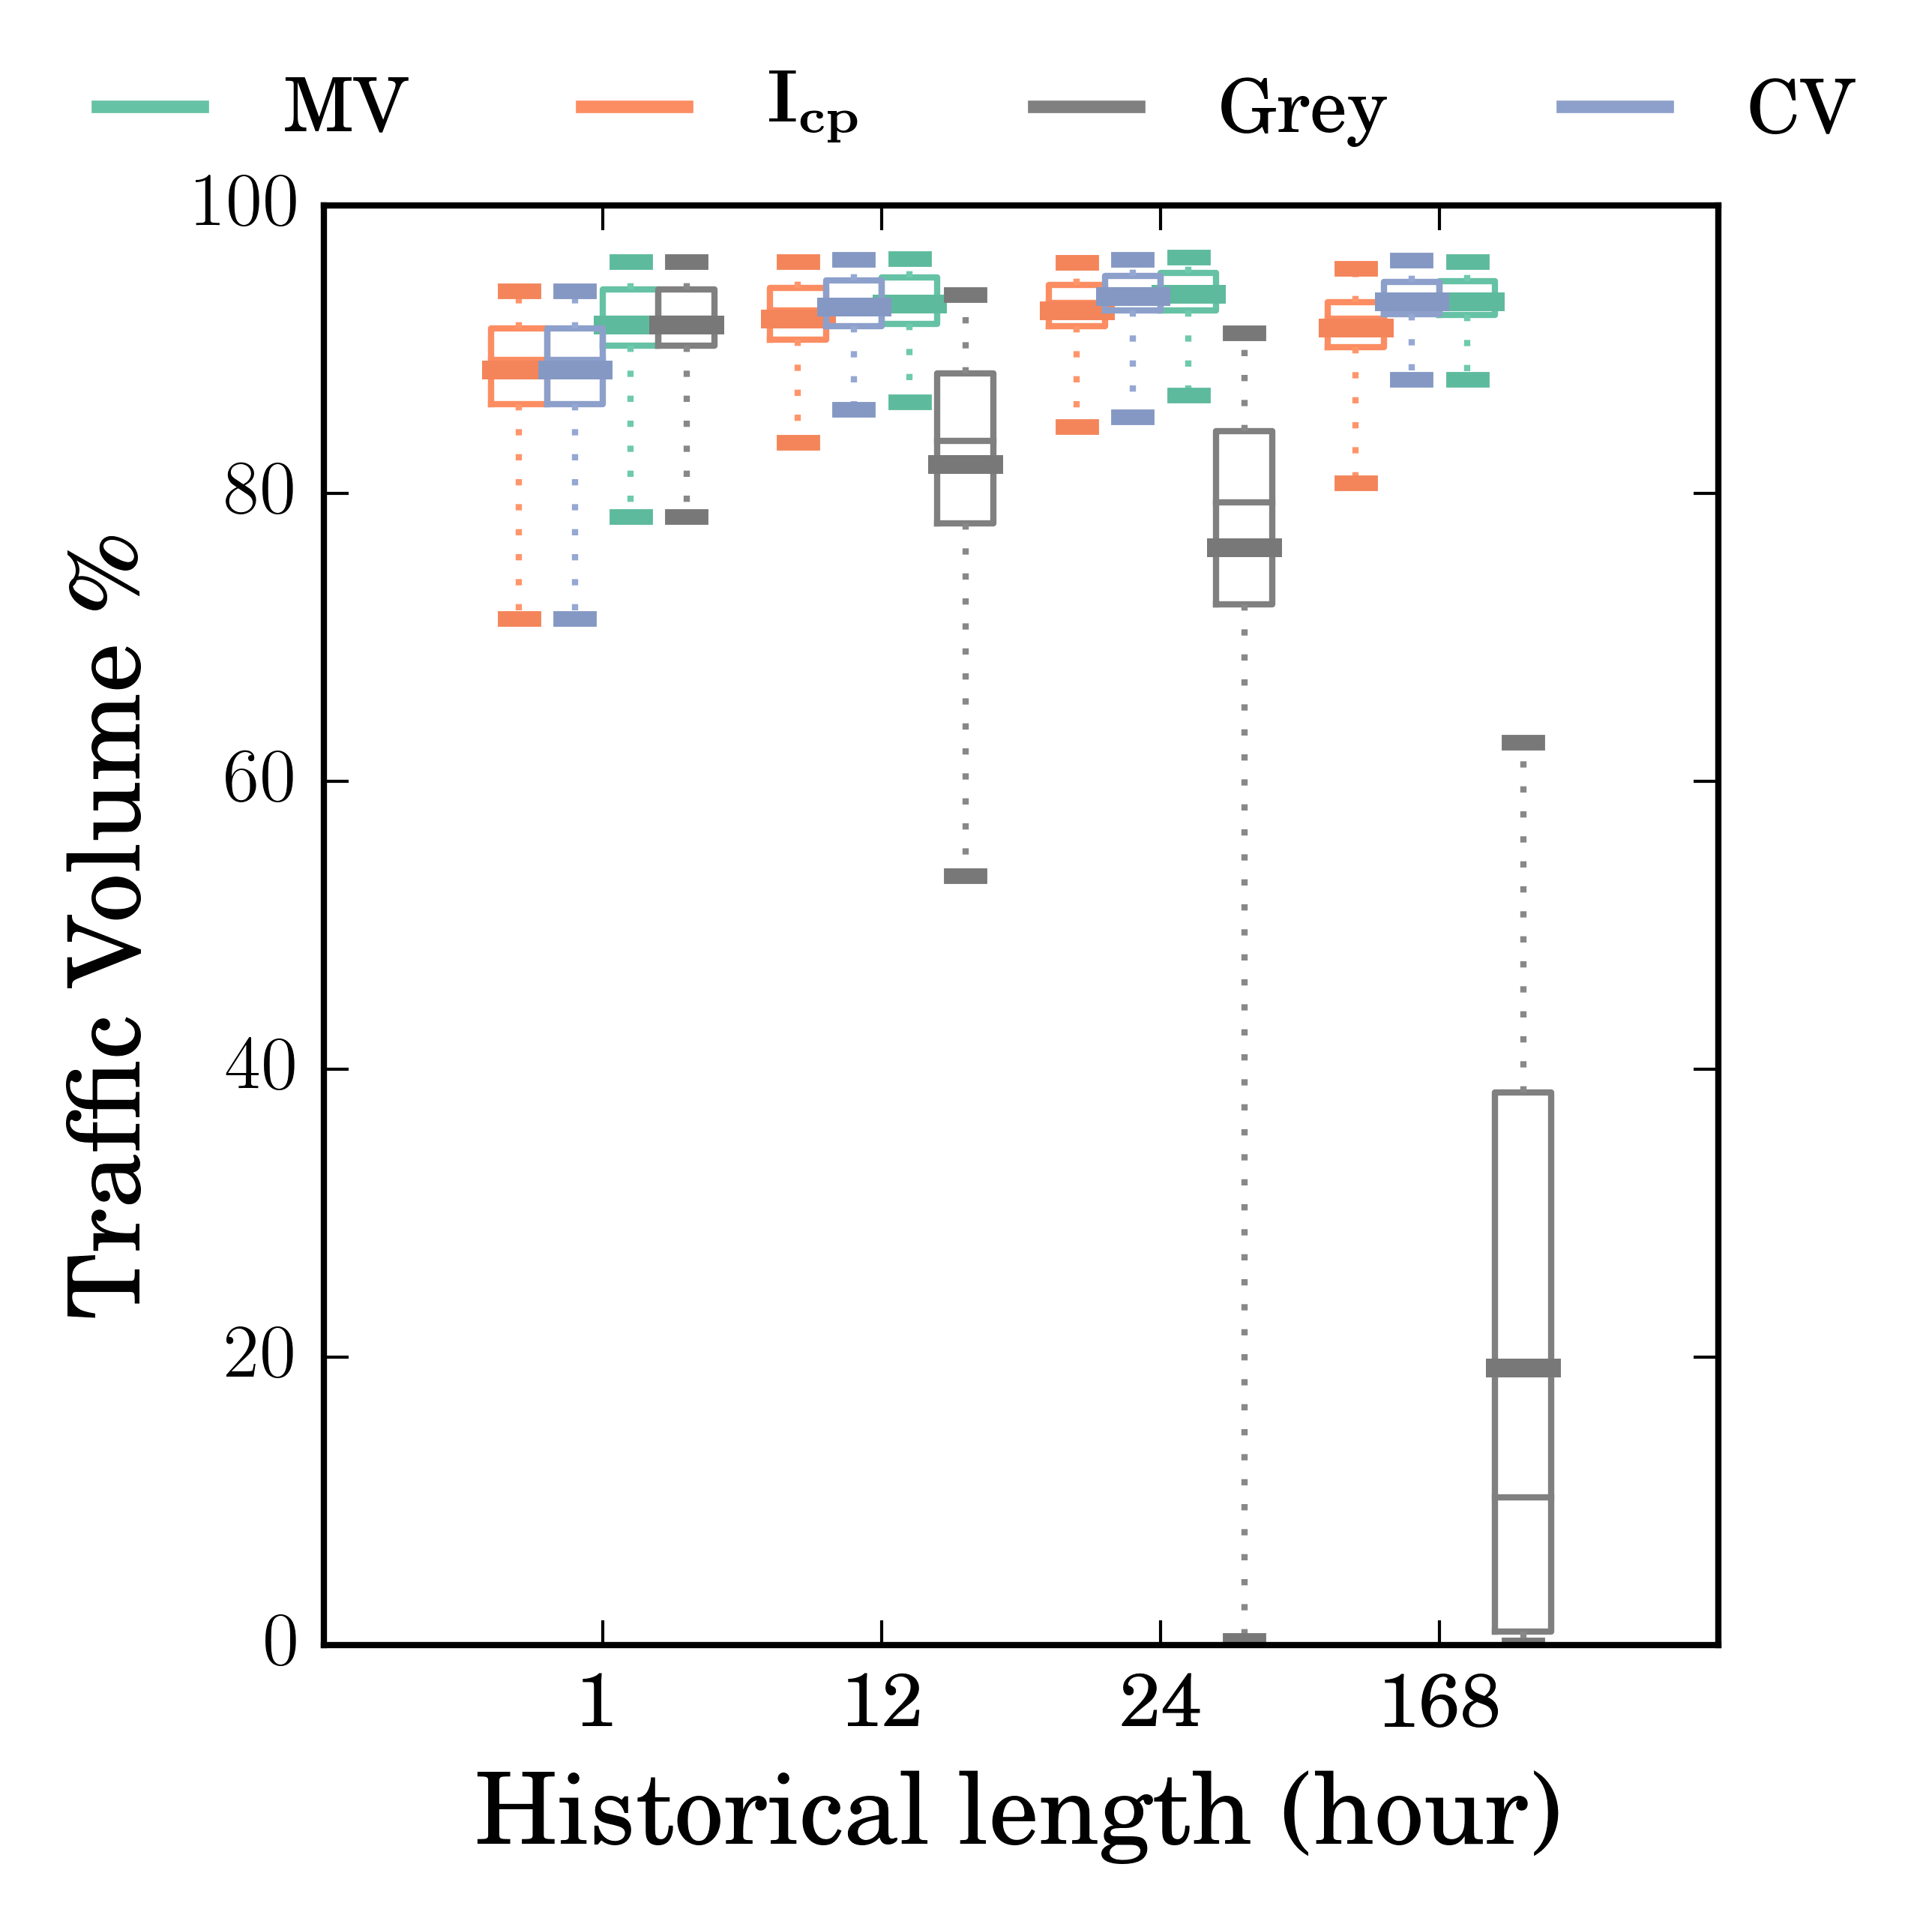
\includegraphics[width=\textwidth]{gfx/chap2/grey_cvg_box_method_compare_fs_sa.png}
                \caption{SA}
                \label{fig:cvg_sa}
        \end{subfigure}
        \begin{subfigure}[b]{0.48\textwidth}
                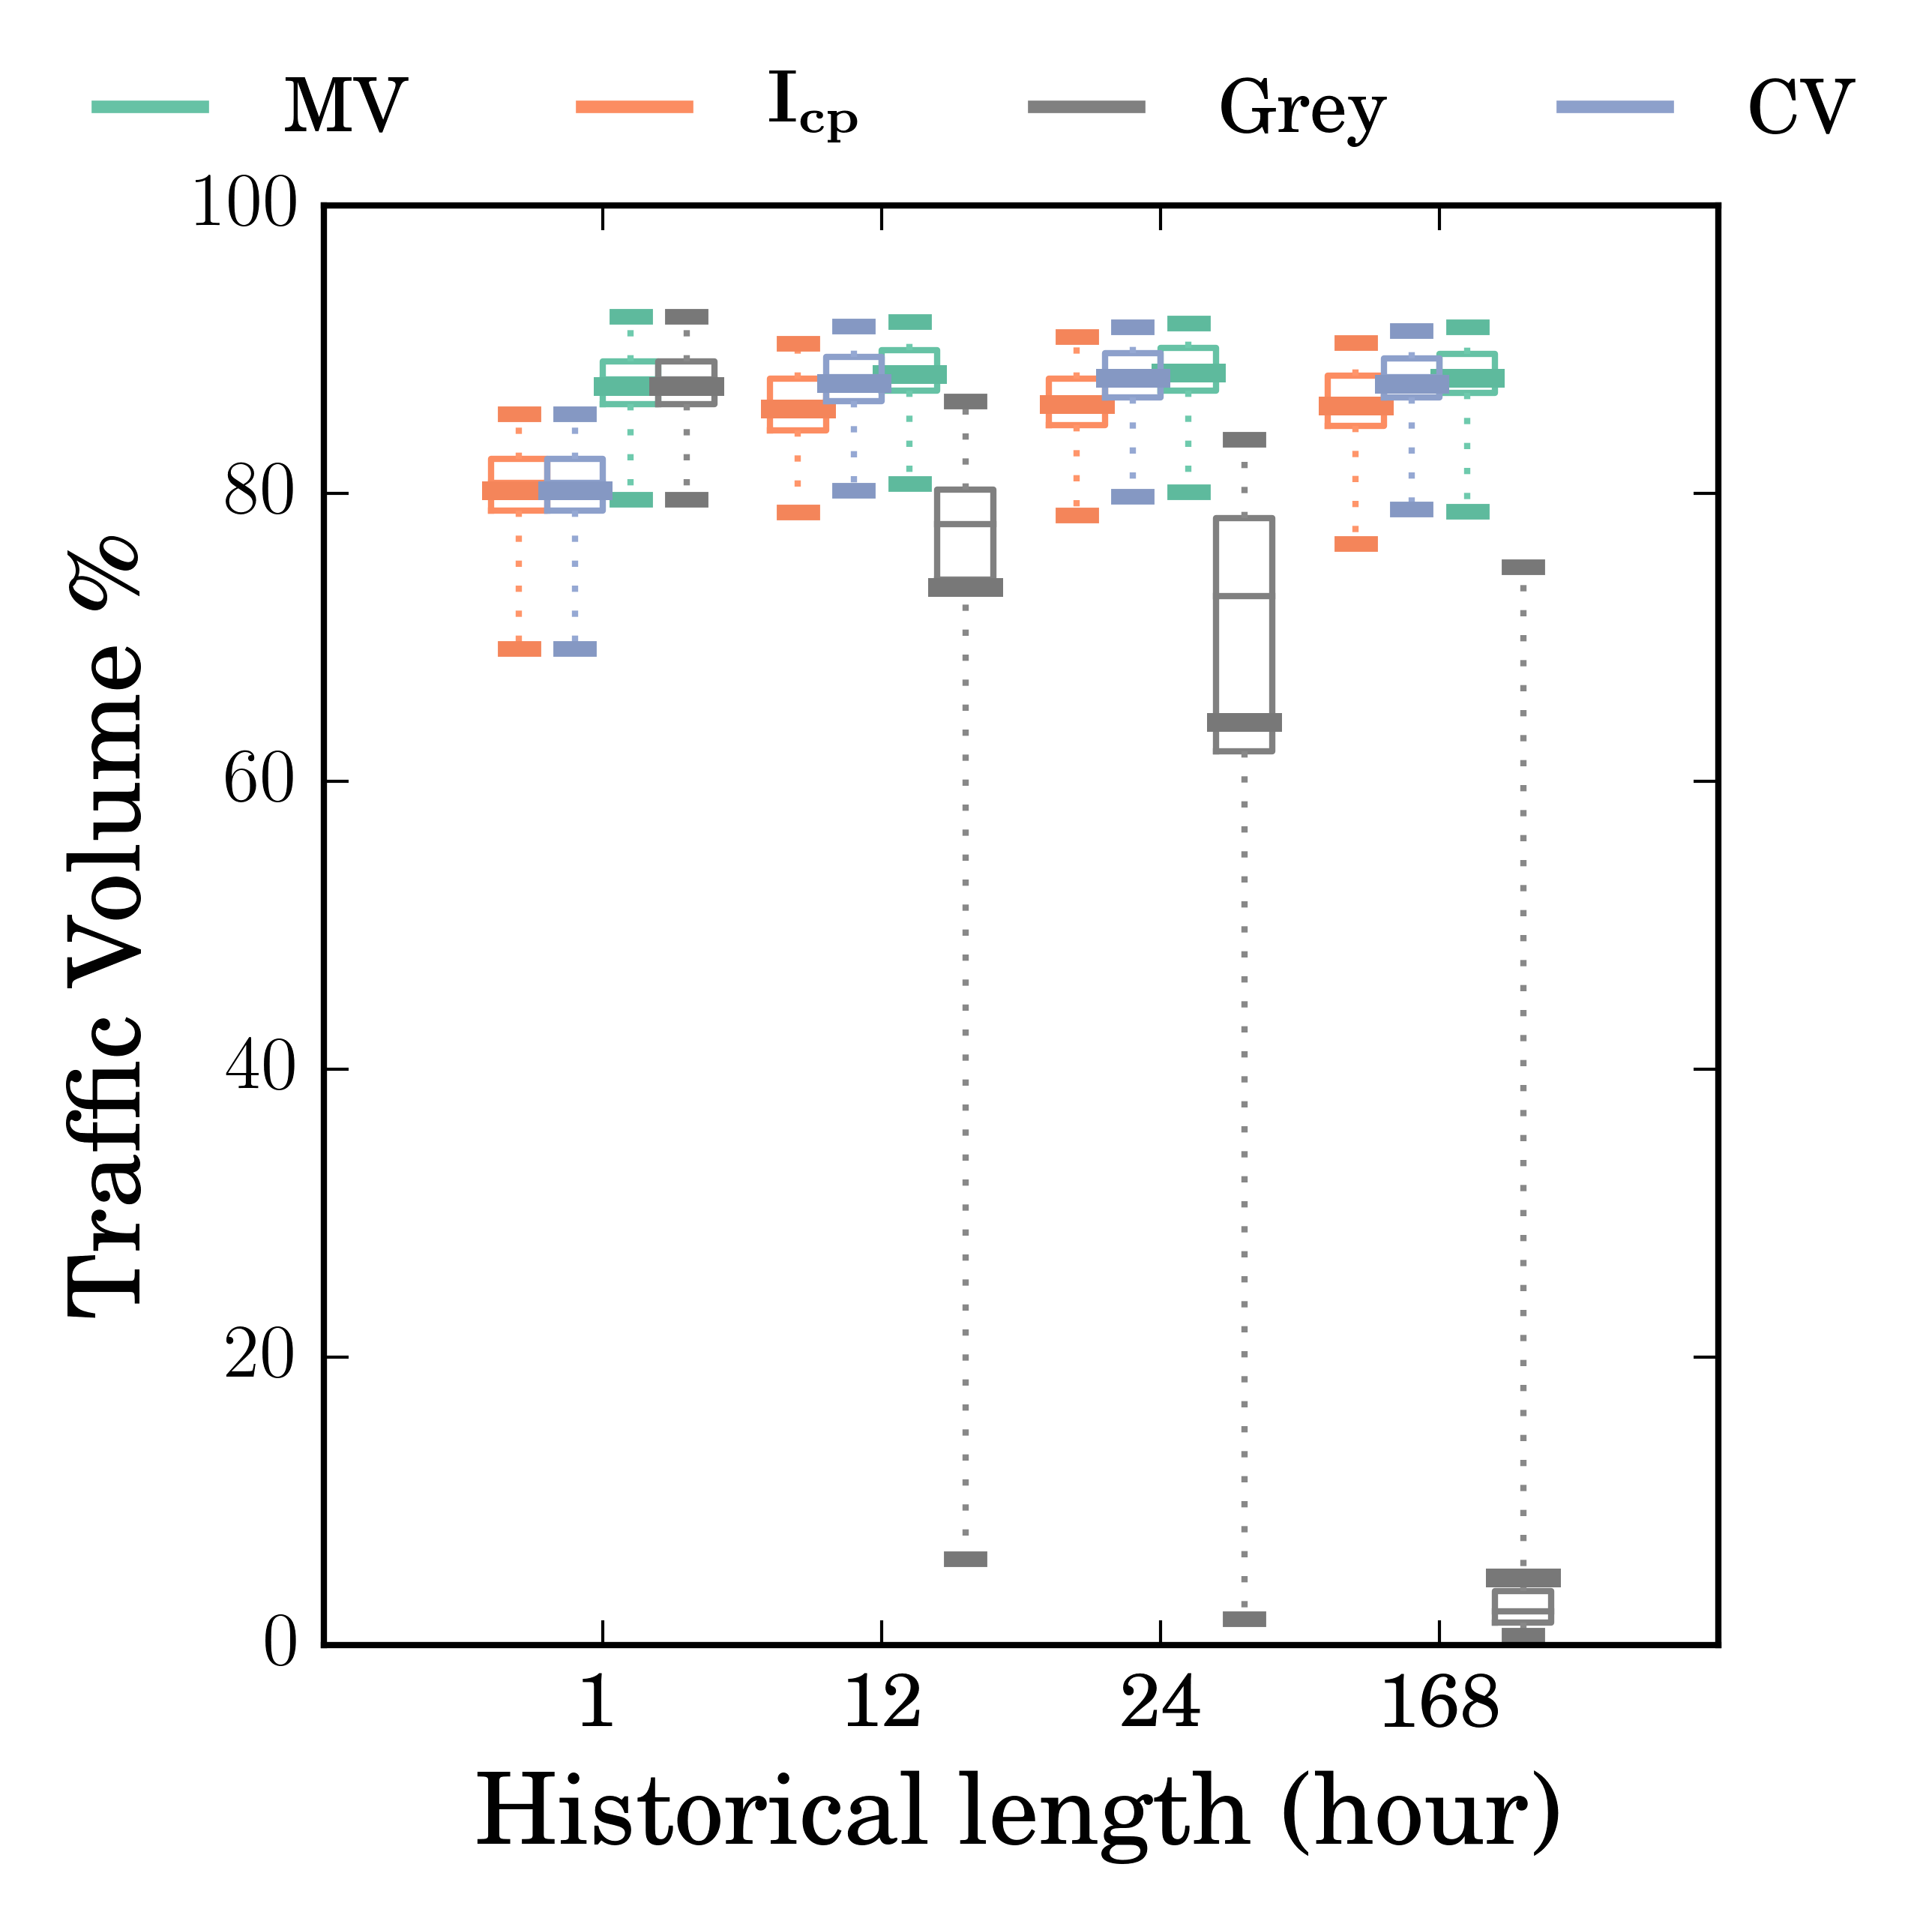
\includegraphics[width=\textwidth]{gfx/chap2/grey_cvg_box_method_compare_fs_sb.png}
                \caption{SB}
                \label{fig:cvg_sb}
        \end{subfigure}
        \begin{subfigure}[b]{0.48\textwidth}
                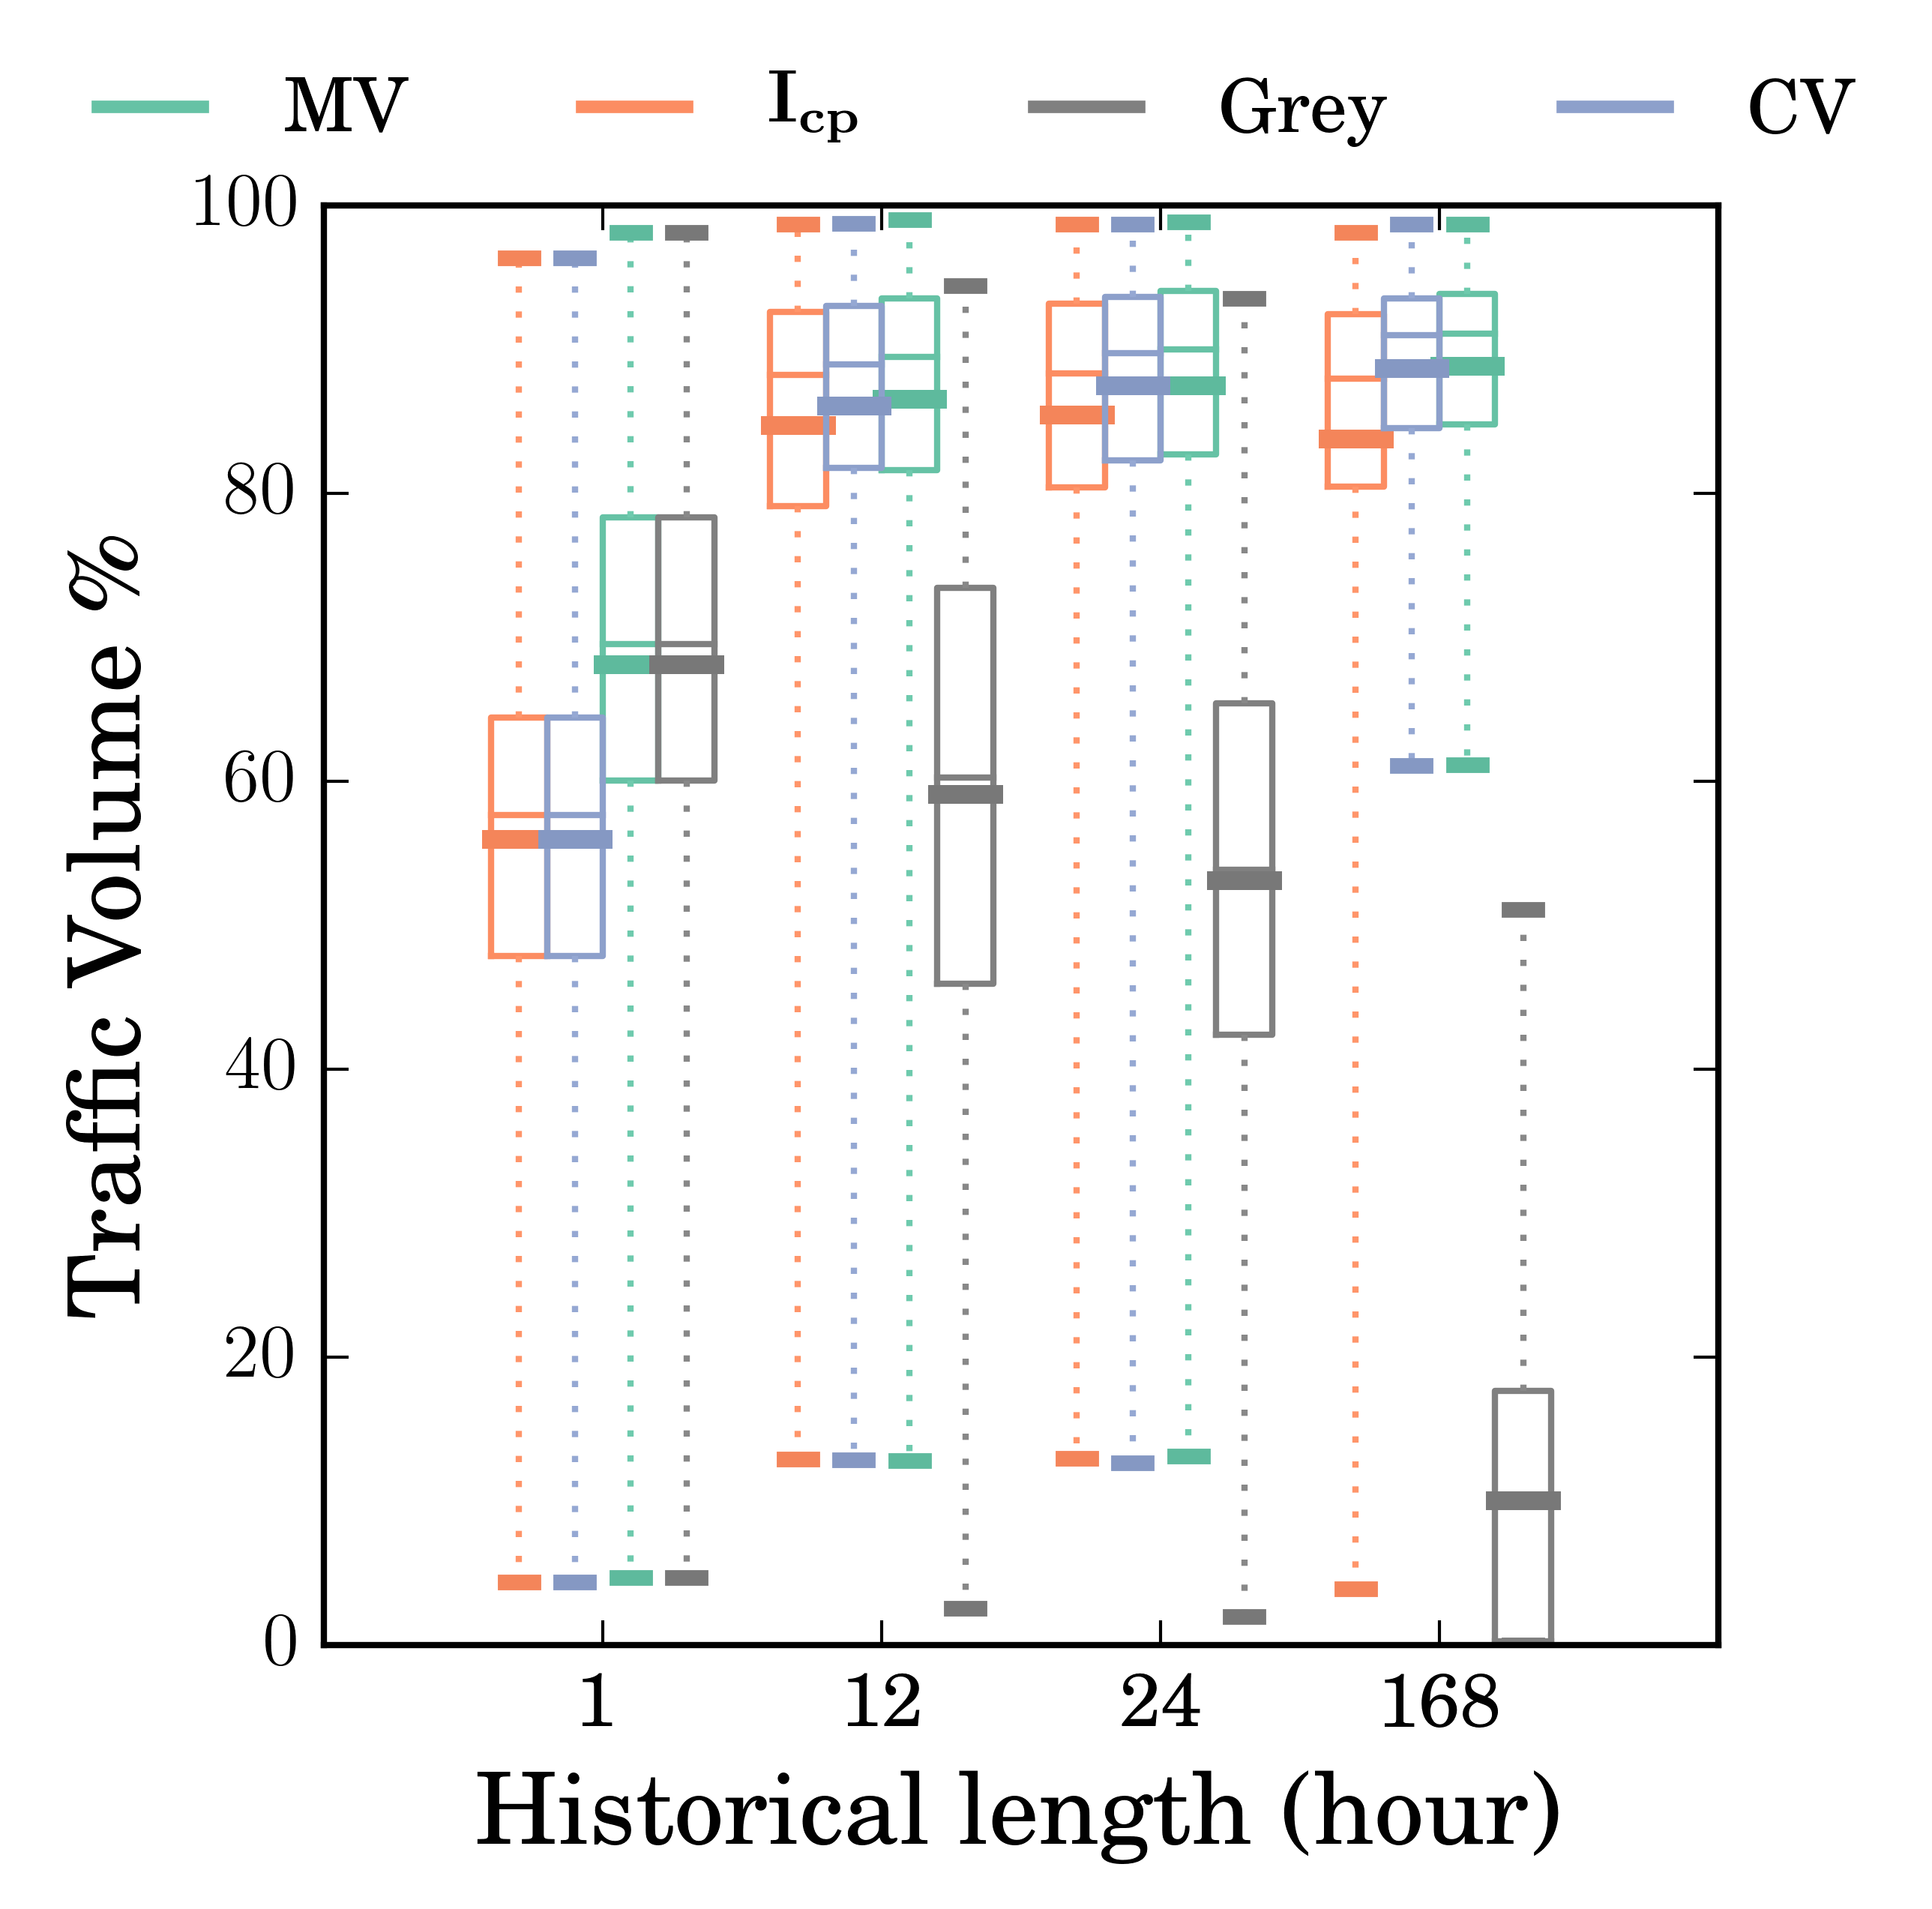
\includegraphics[width=\textwidth]{gfx/chap2/grey_cvg_box_method_compare_fs_sc.png}
                \caption{SC}
                \label{fig:cvg_sc}
        \end{subfigure}
        \begin{subfigure}[b]{0.48\textwidth}
                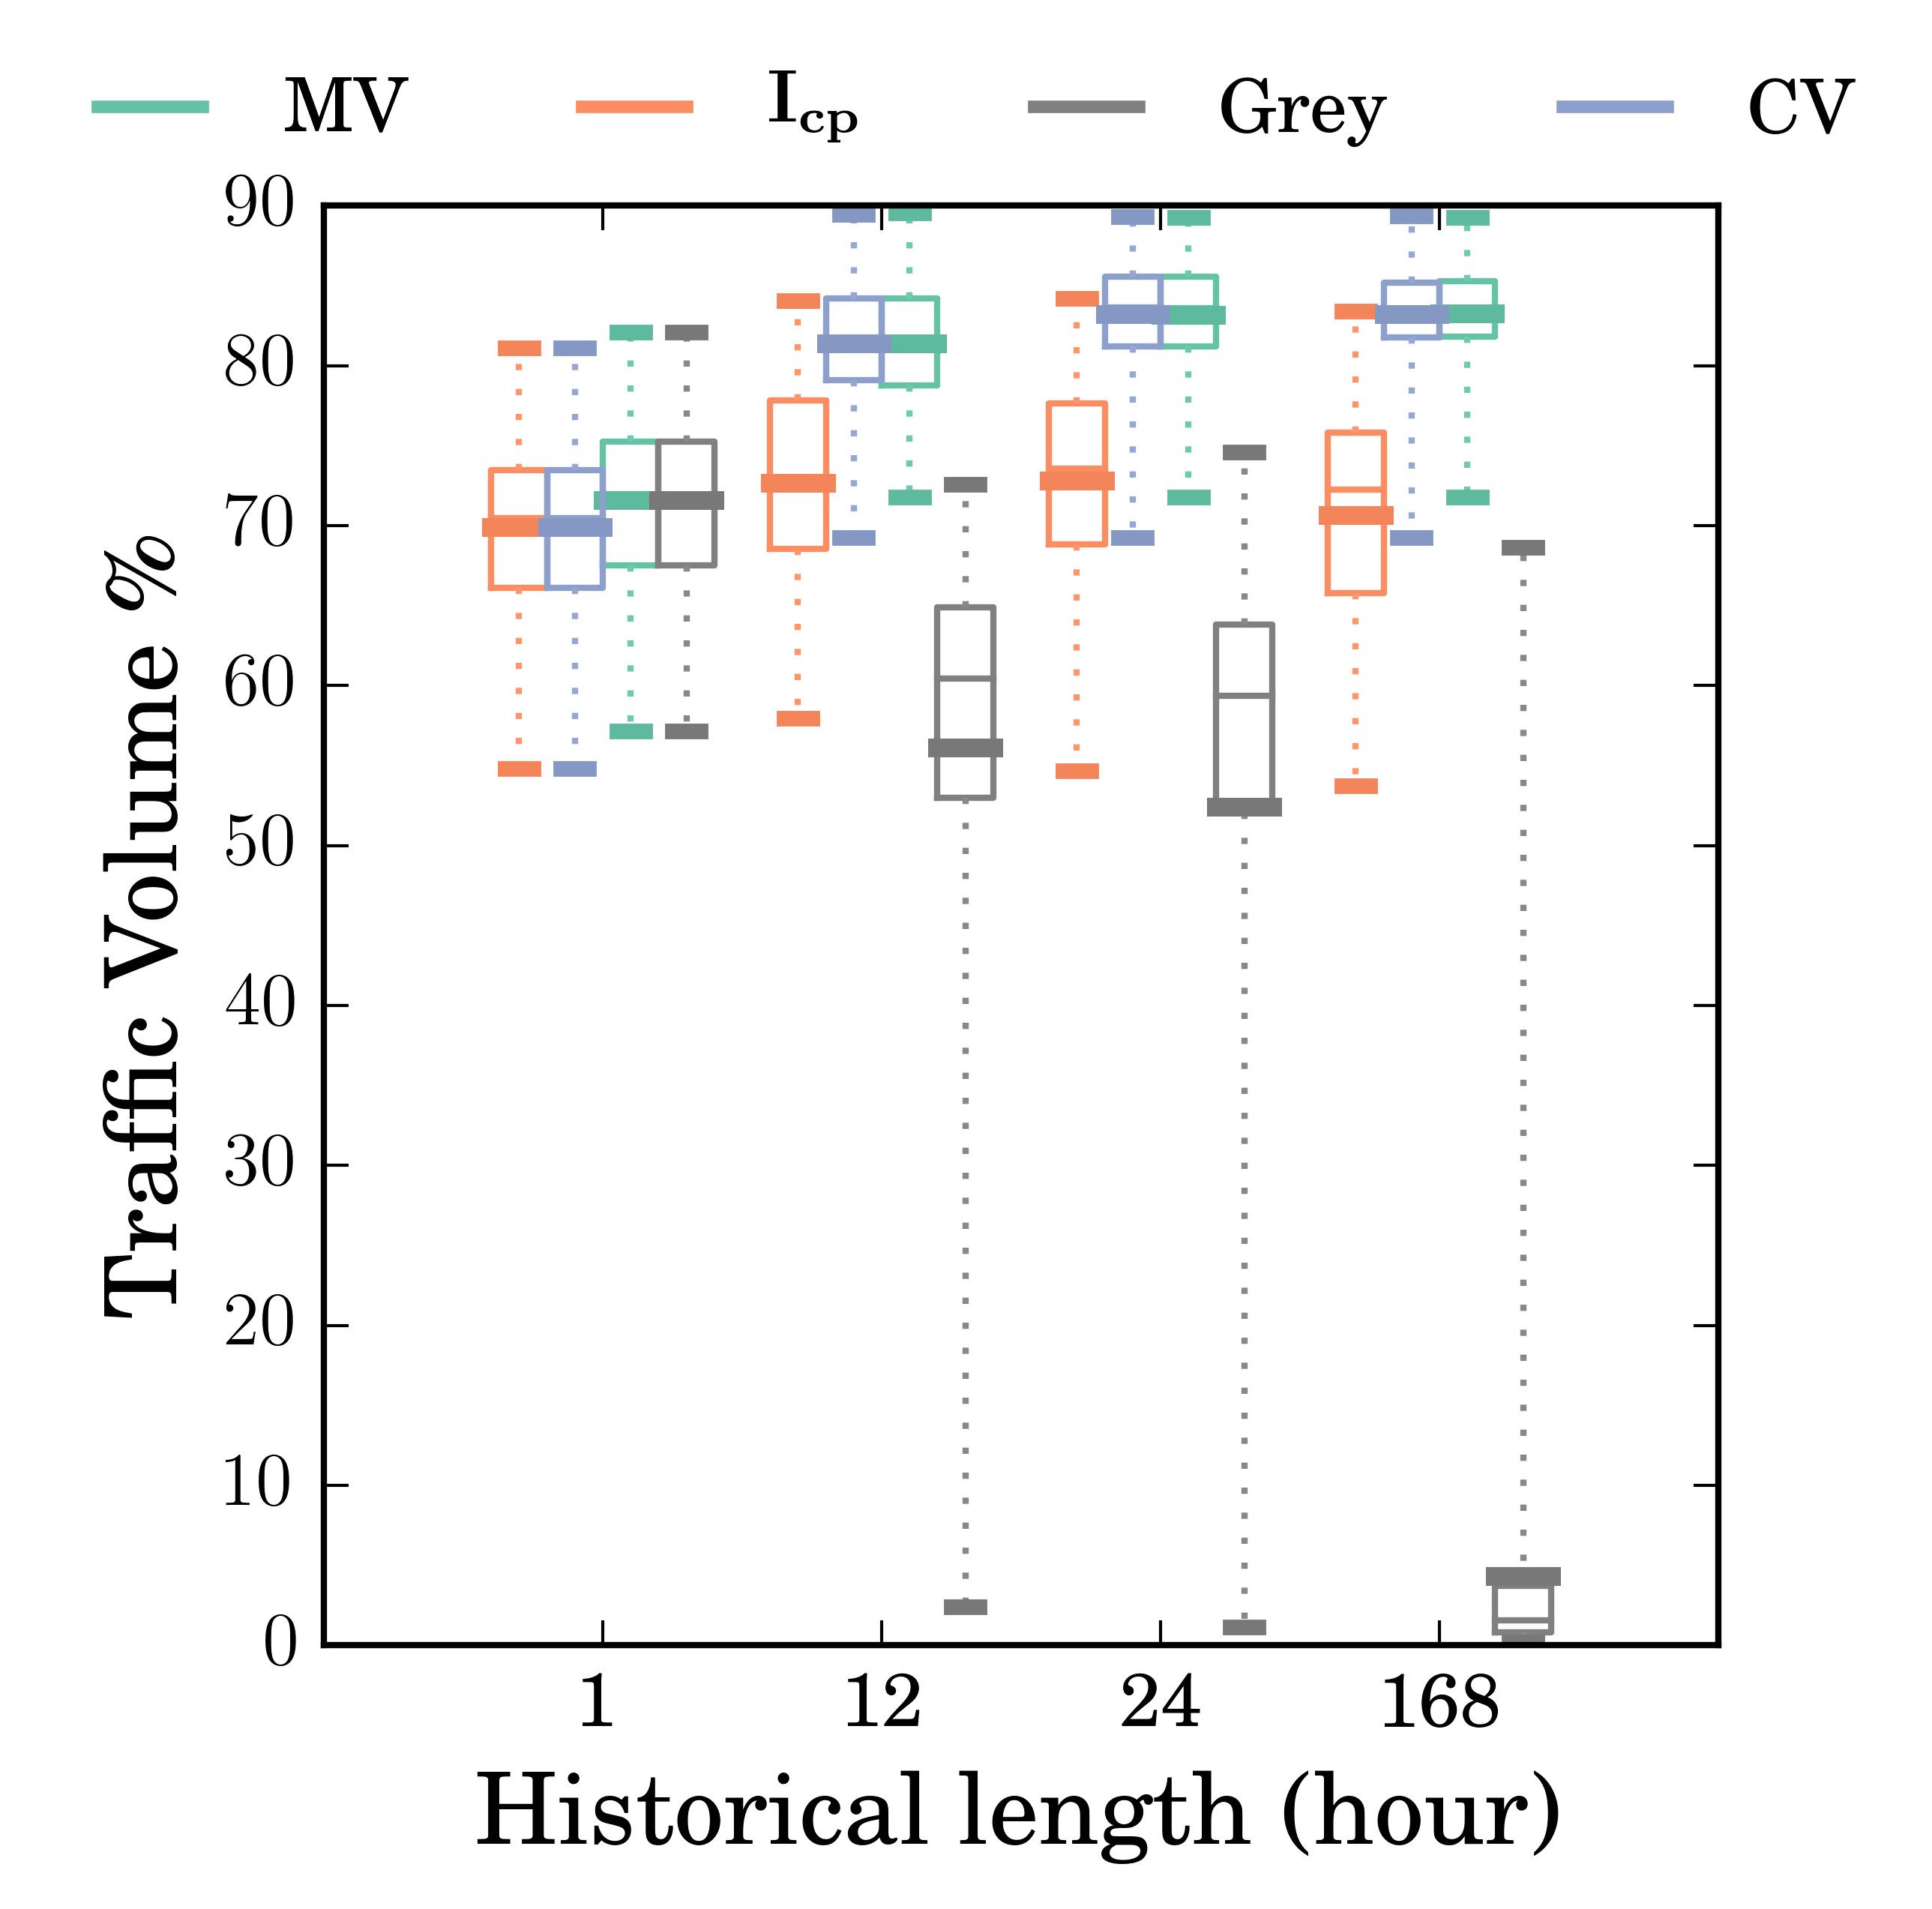
\includegraphics[width=\textwidth]{gfx/chap2/grey_cvg_box_method_compare_fs_sd.png}
                \caption{SD}
                \label{fig:cvg_sd}
        \end{subfigure}
        \begin{subfigure}[b]{0.48\textwidth}
                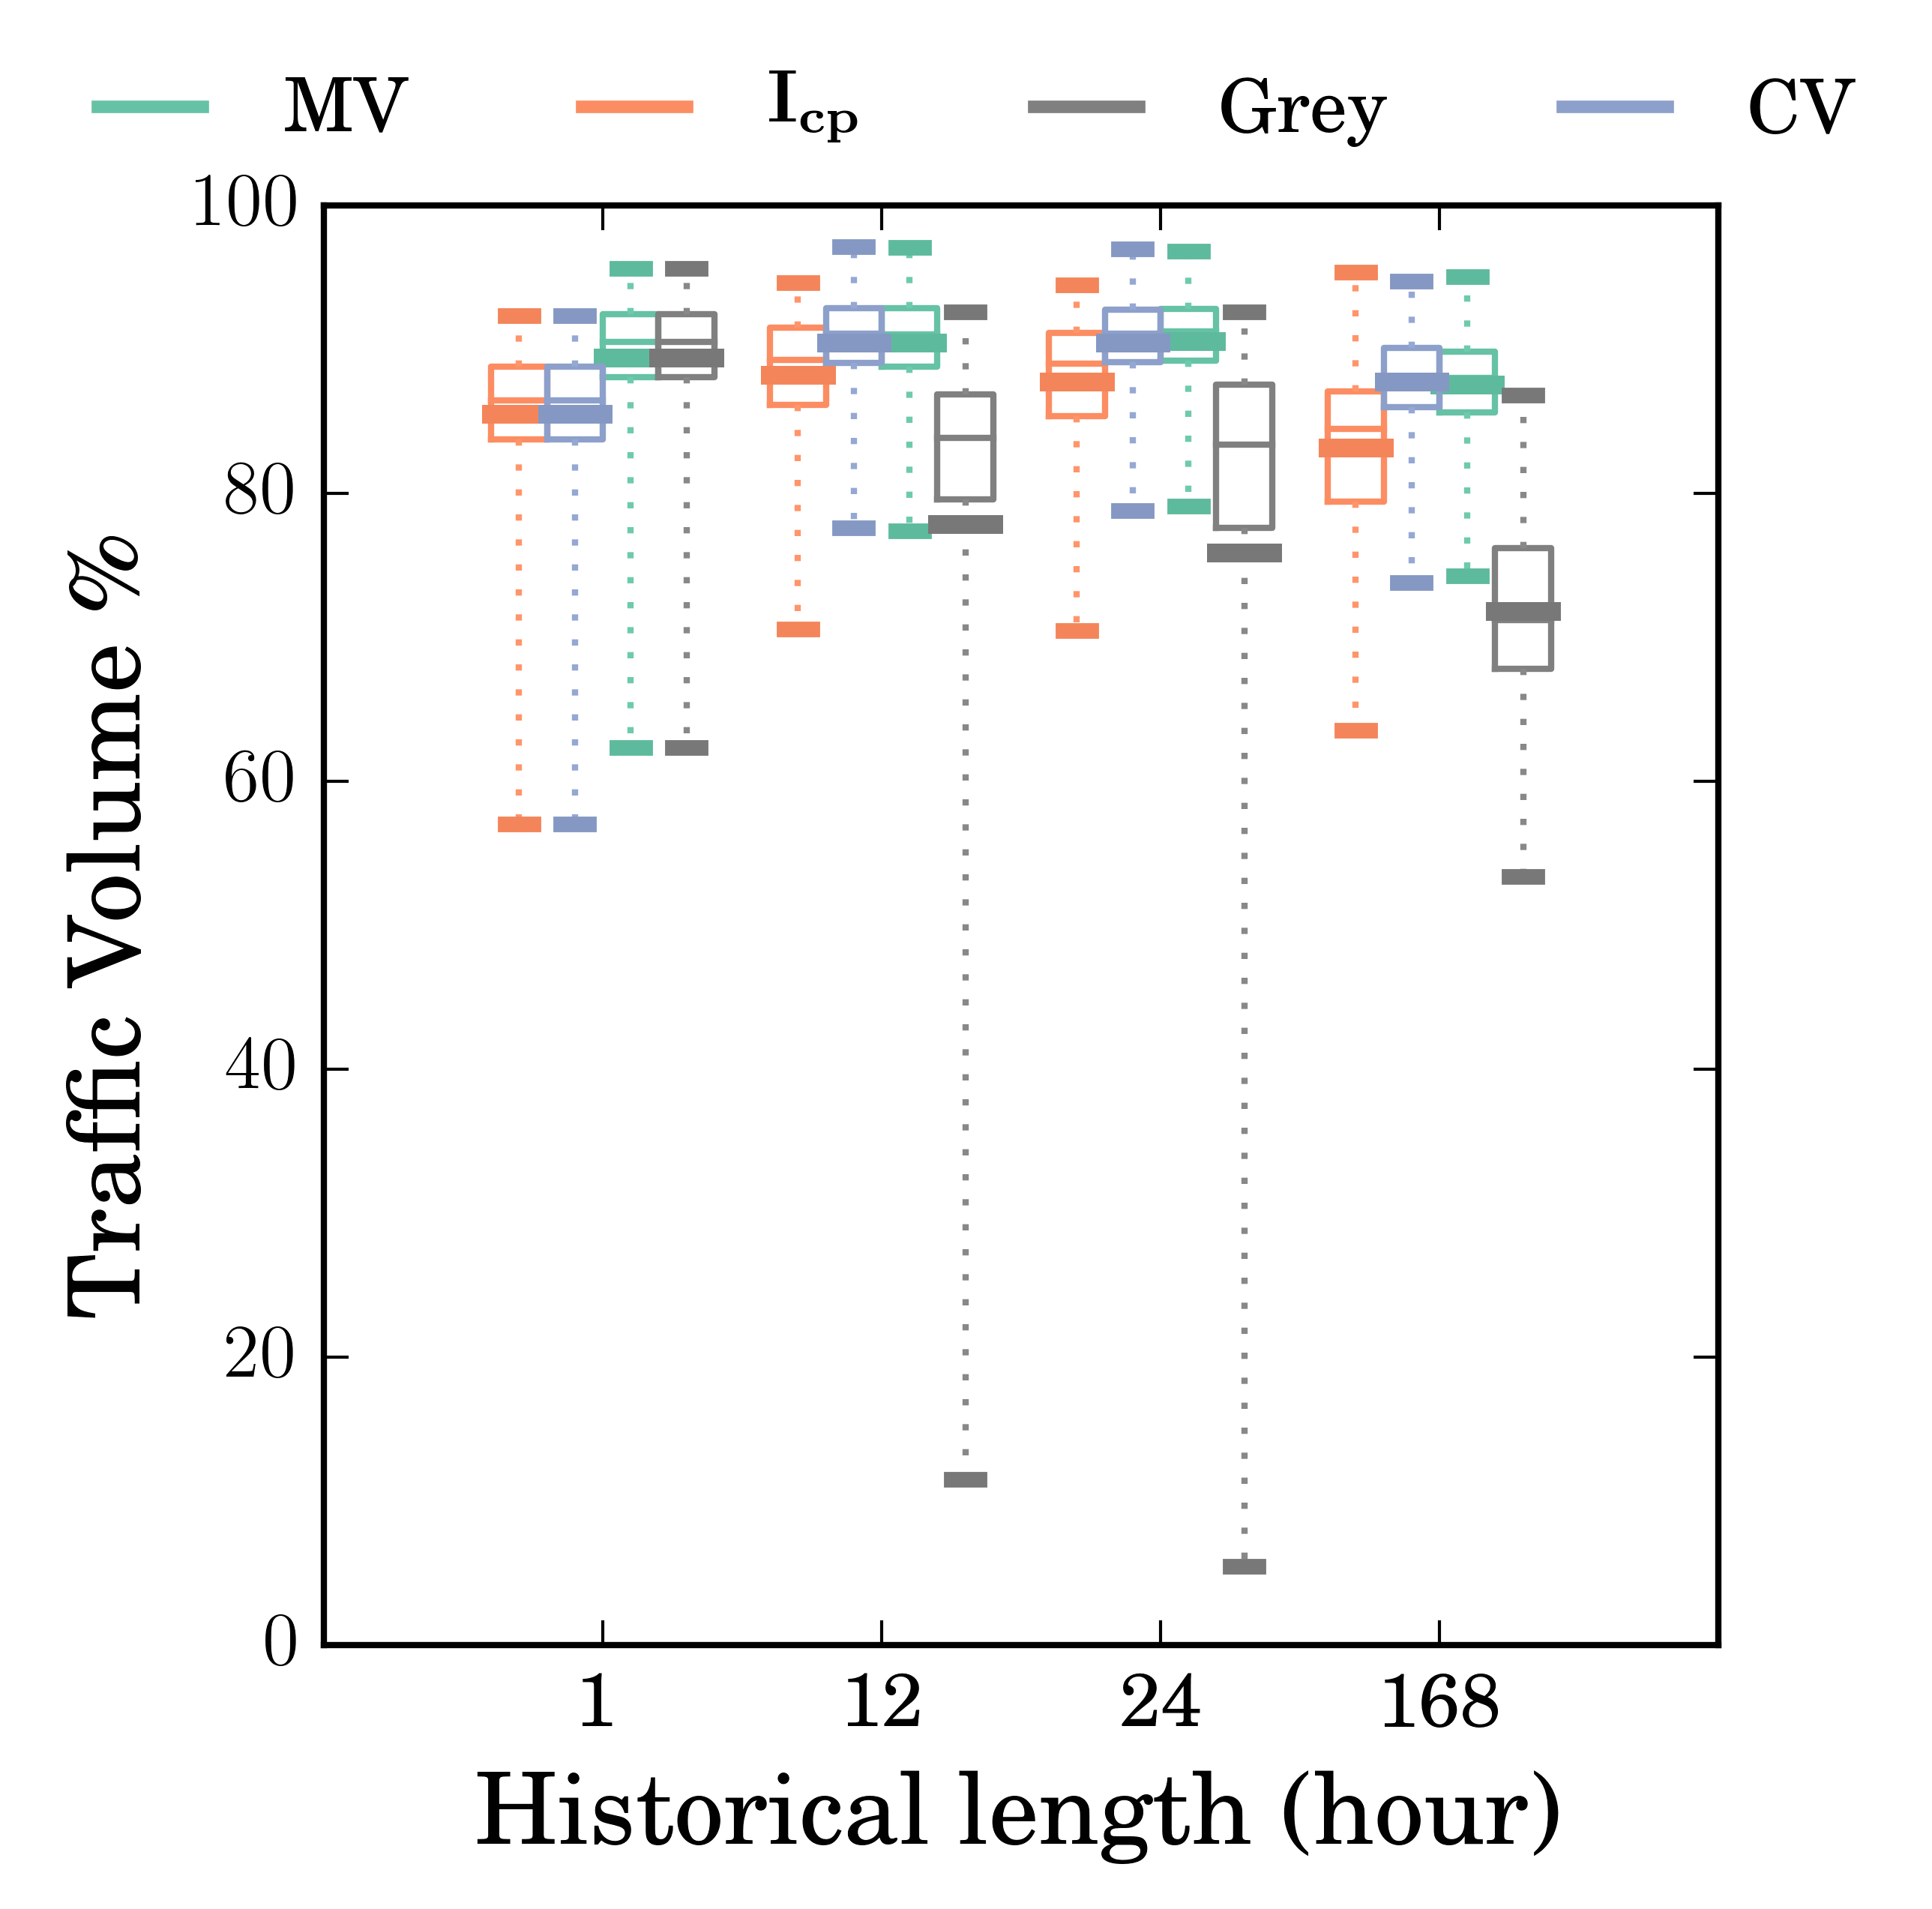
\includegraphics[width=\textwidth]{gfx/chap2/grey_cvg_box_method_compare_fs_se.png}
                \caption{SE}
                \label{fig:cvg_se}
        \end{subfigure}
        \begin{subfigure}[b]{0.48\textwidth}
                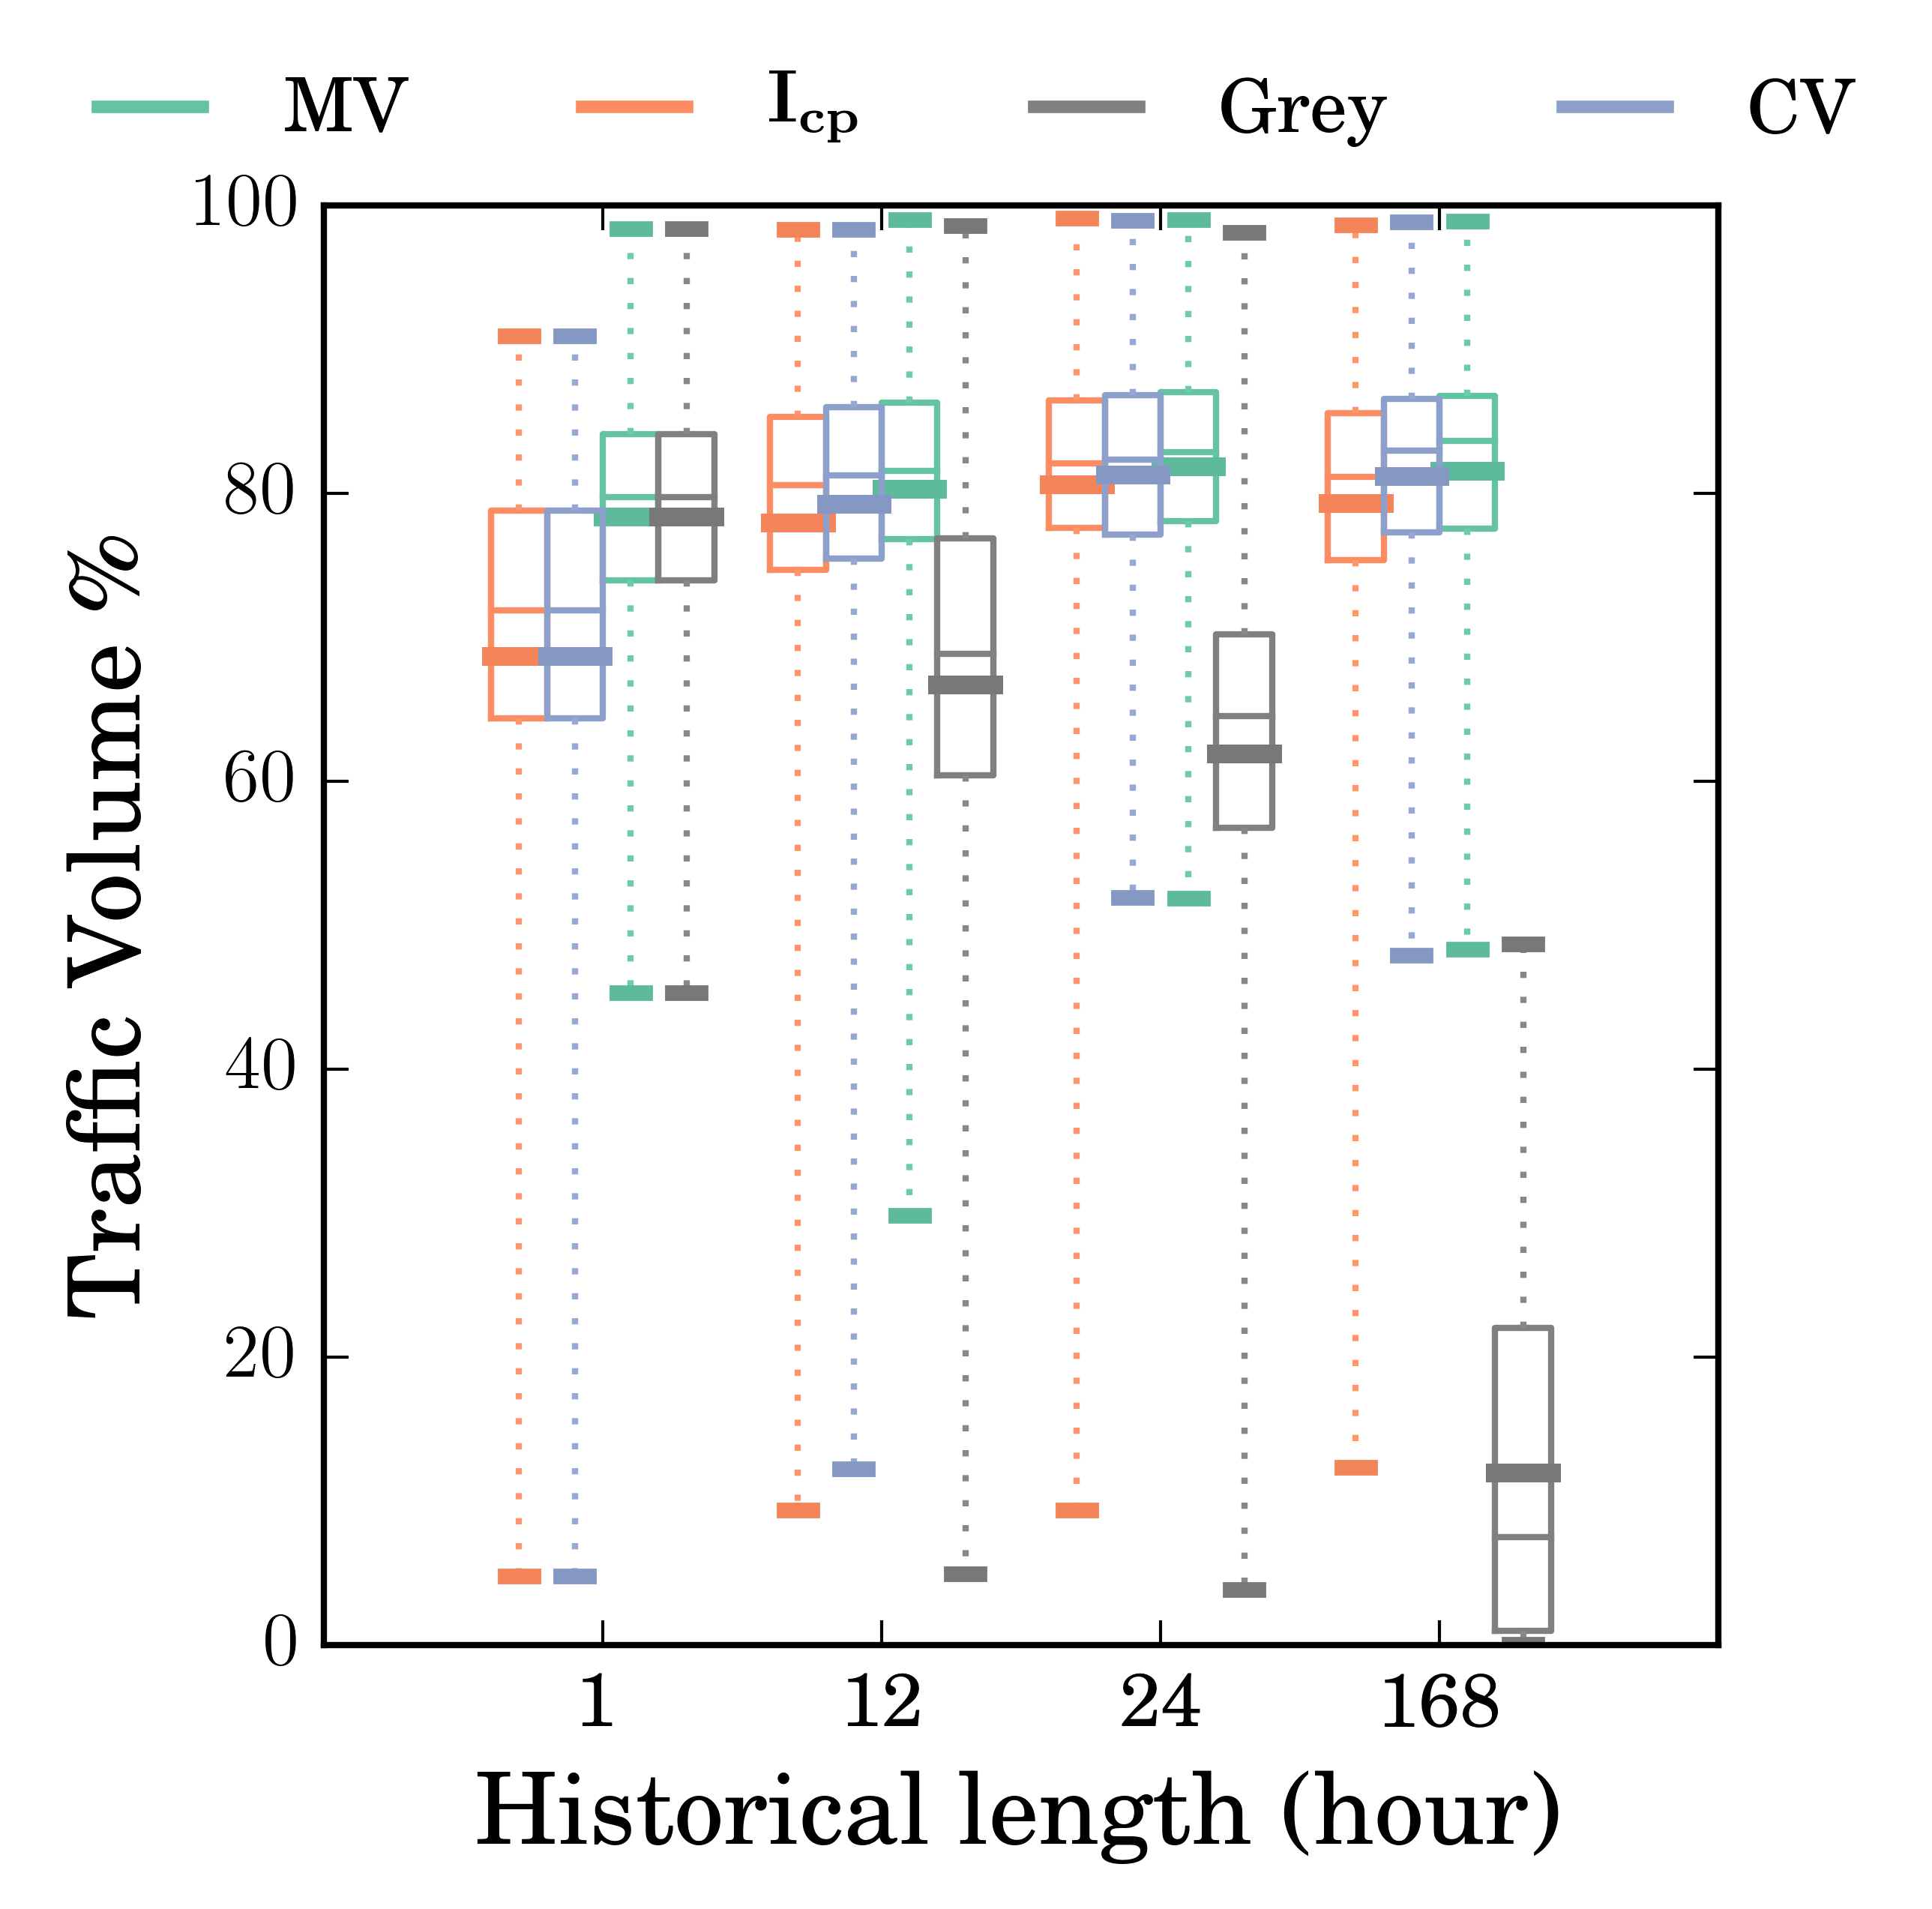
\includegraphics[width=\textwidth]{gfx/chap2/grey_cvg_box_method_compare_fs_sf.png}
                \caption{SF}
                \label{fig:cvg_sf}
        \end{subfigure}
\caption{Hour volume fraction covered by prefixes predictively selected using historical records of different lengths. The selection set size of each network is set to the maximum \textit{core} size over the week starting from June 1st, 2015, see in Table~\ref{tab:core_size}.}
\label{fig:cvg}
\end{figure}

\begin{figure}\ContinuedFloat
	\centering
        \begin{subfigure}[b]{0.48\textwidth}
                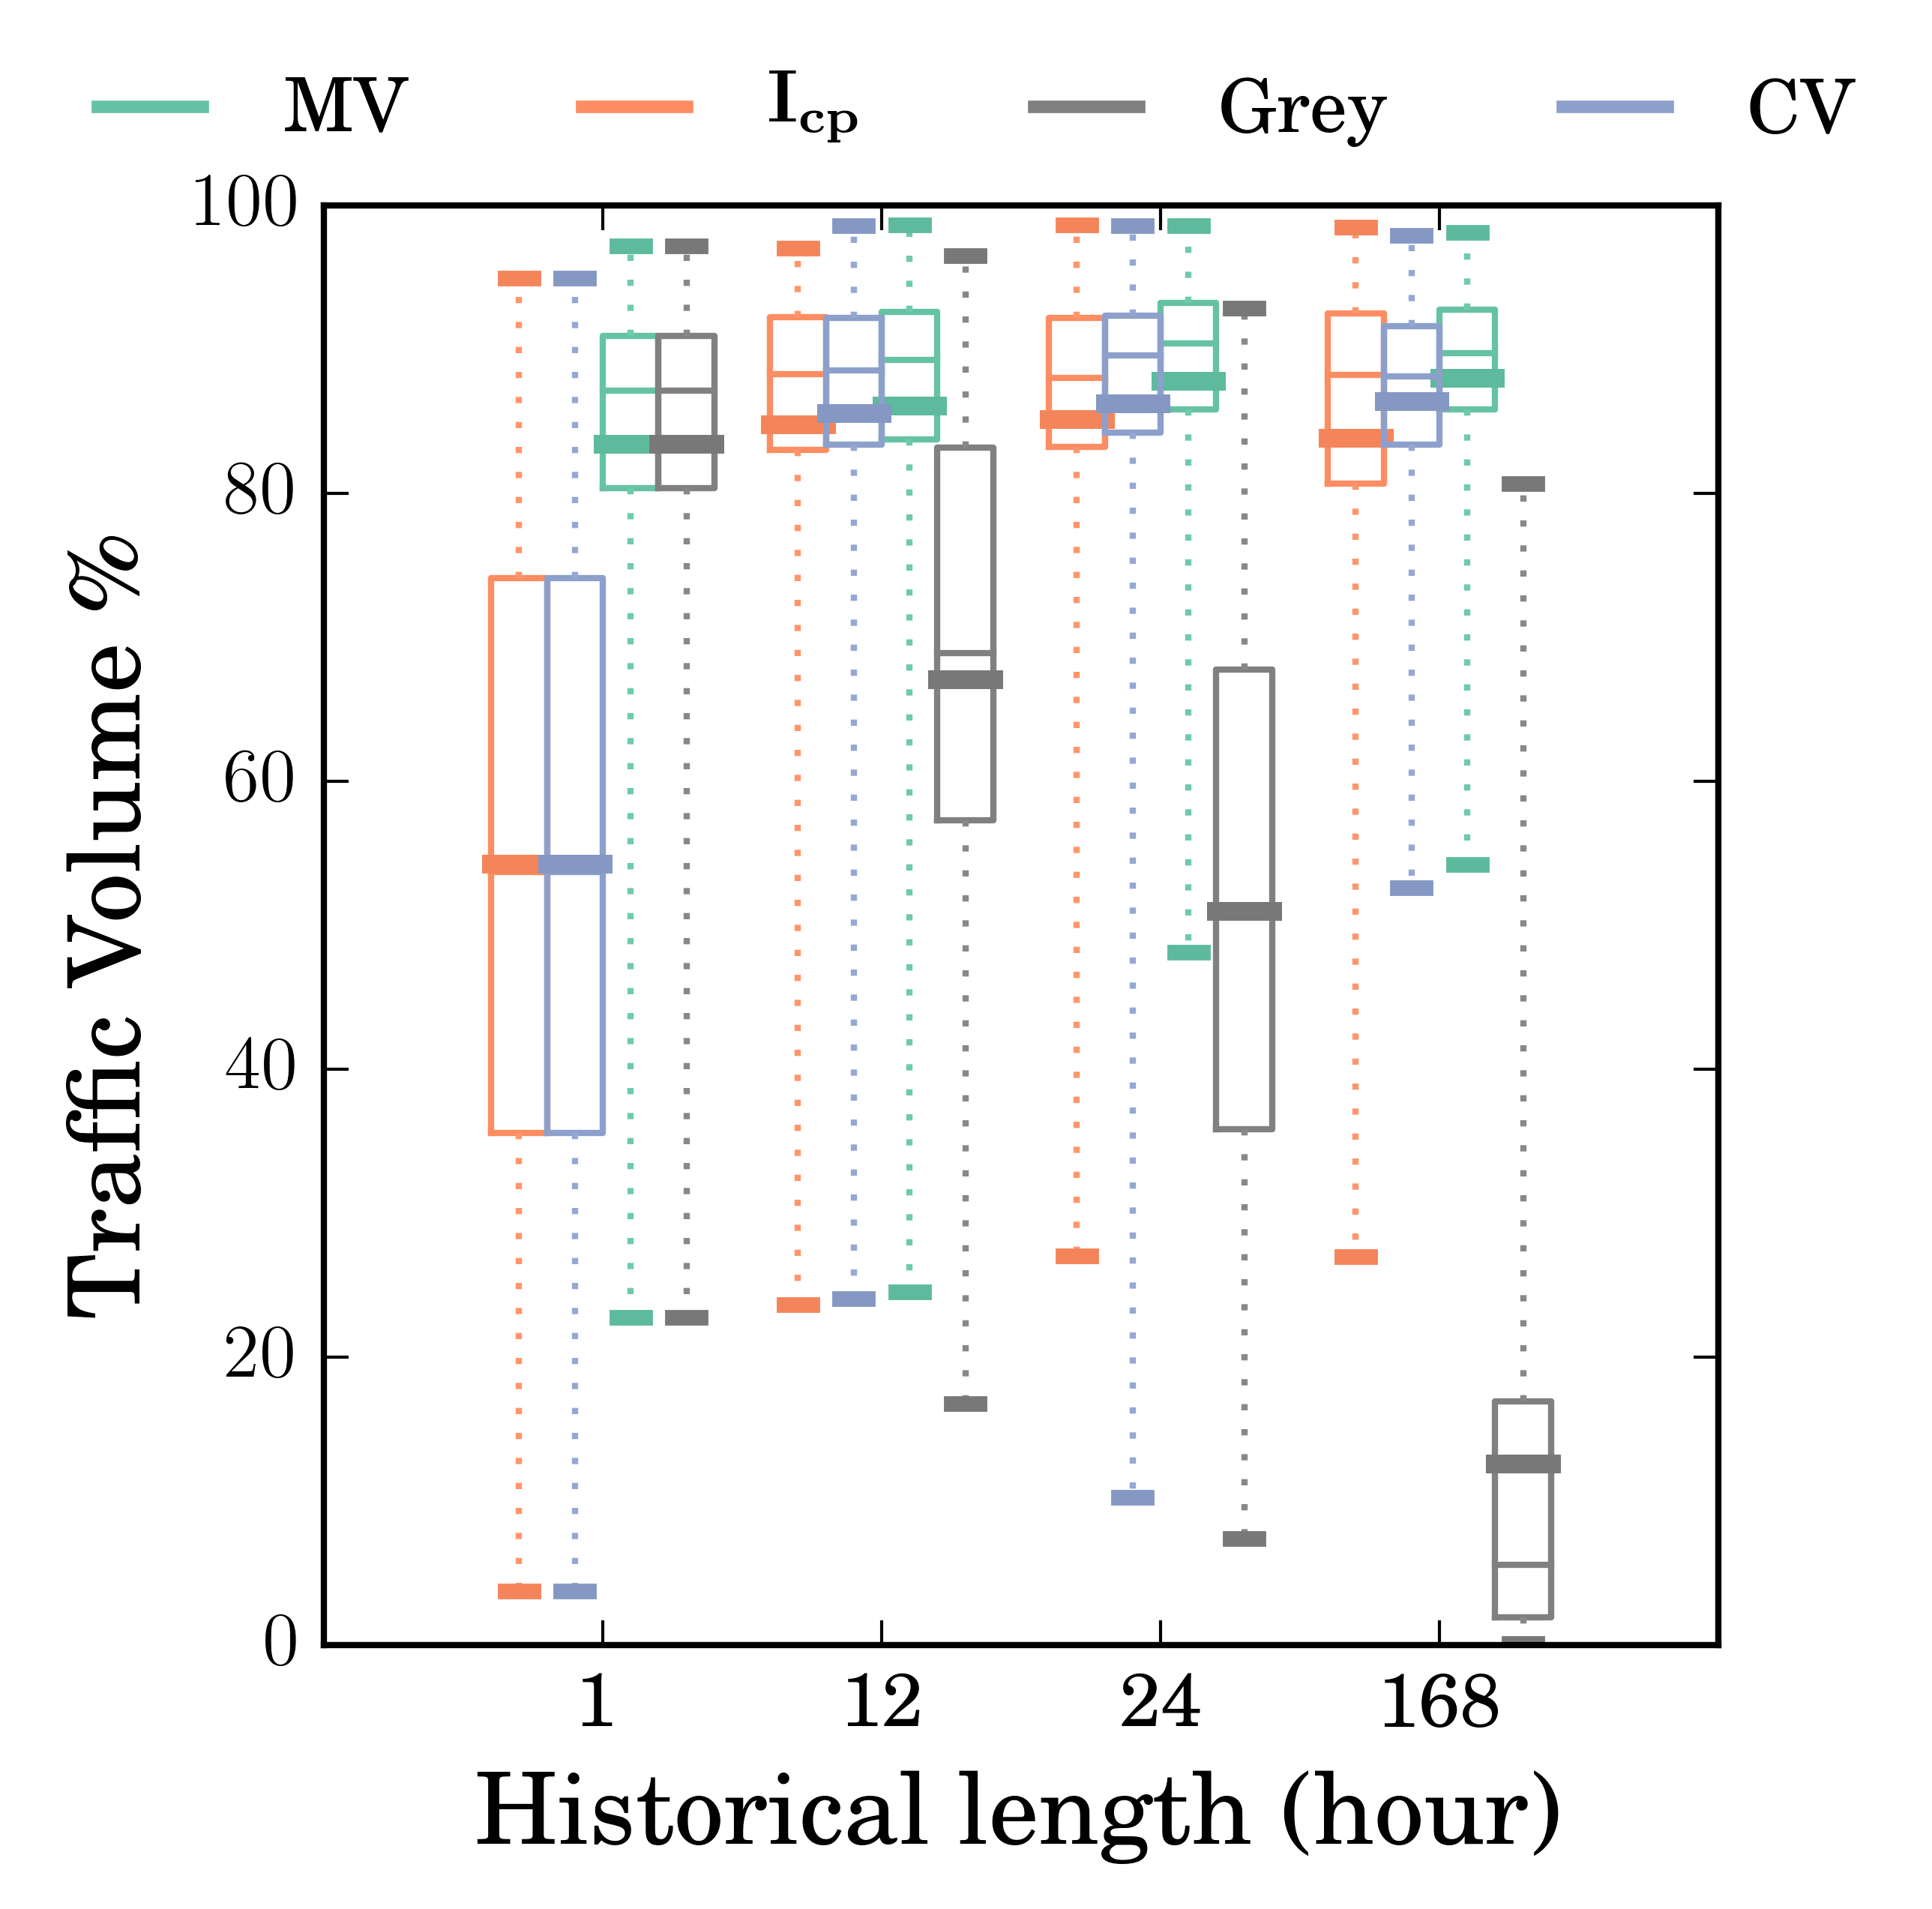
\includegraphics[width=\textwidth]{gfx/chap2/grey_cvg_box_method_compare_fs_sg.png}
                \caption{SG}
                \label{fig:cvg_sg}
        \end{subfigure}
        \begin{subfigure}[b]{0.48\textwidth}
                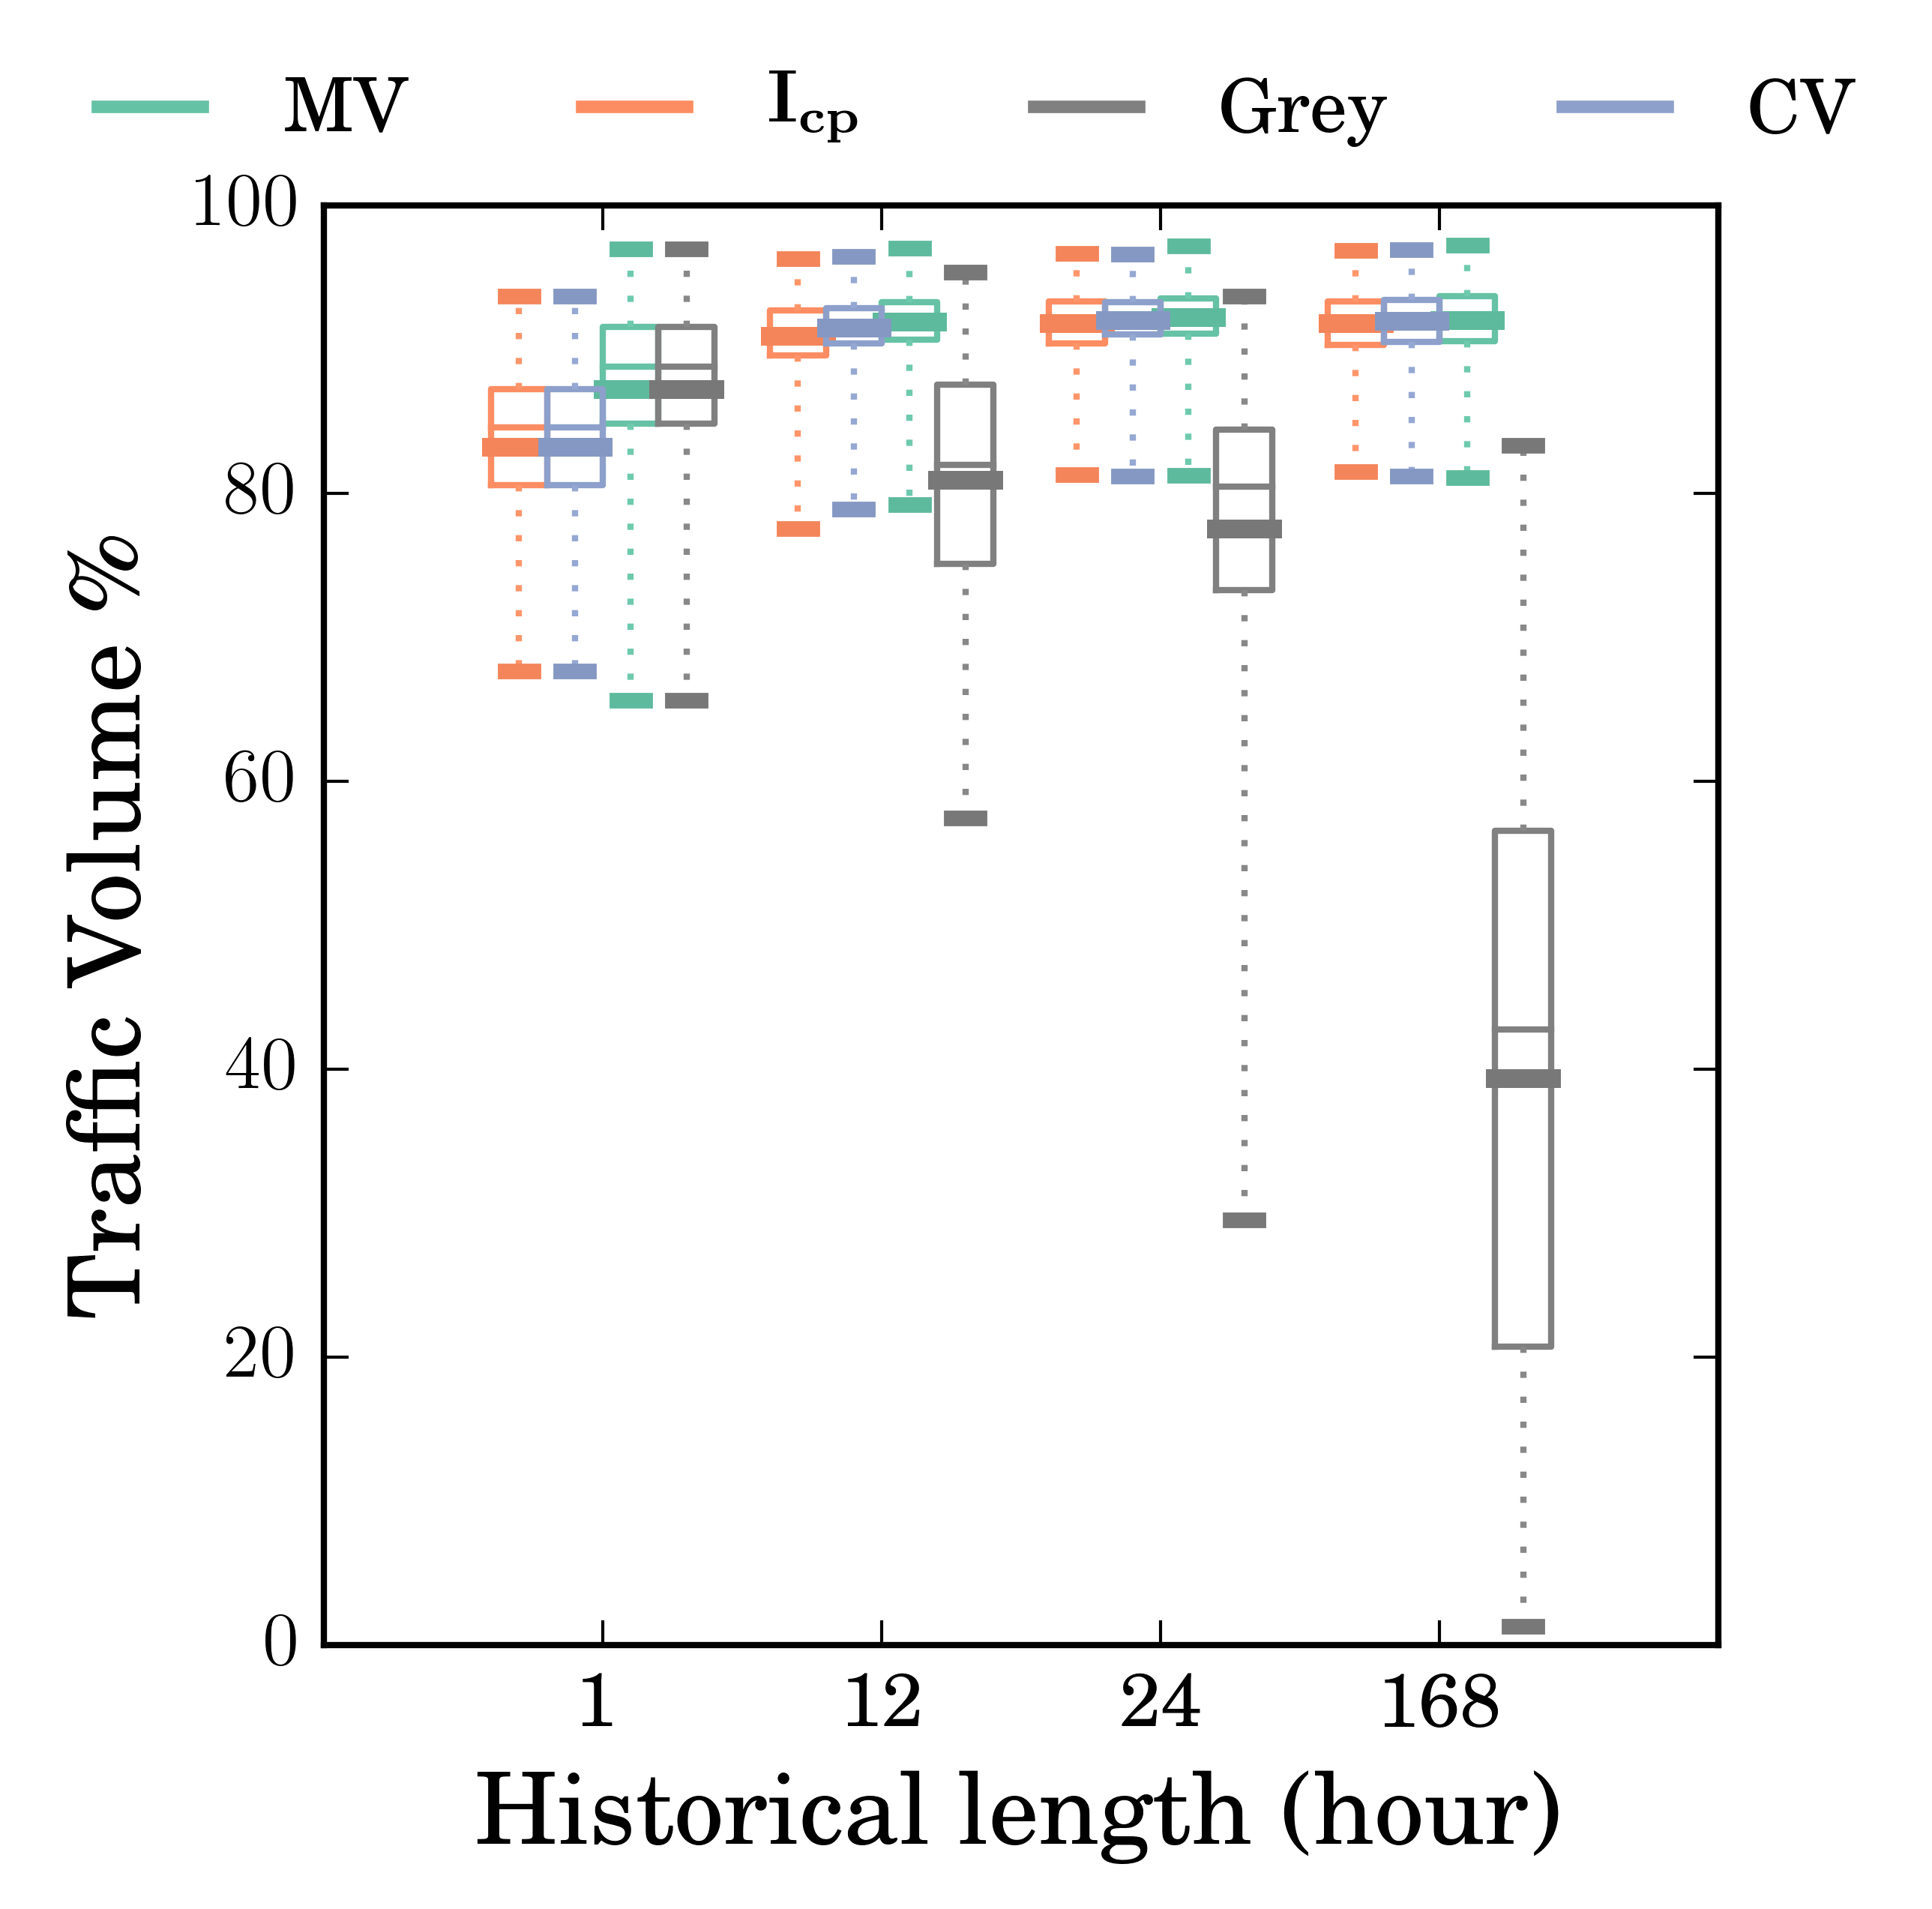
\includegraphics[width=\textwidth]{gfx/chap2/grey_cvg_box_method_compare_fs_sh.png}
                \caption{SH}
                \label{fig:cvg_sh}
        \end{subfigure}
        \begin{subfigure}[b]{0.48\textwidth}
                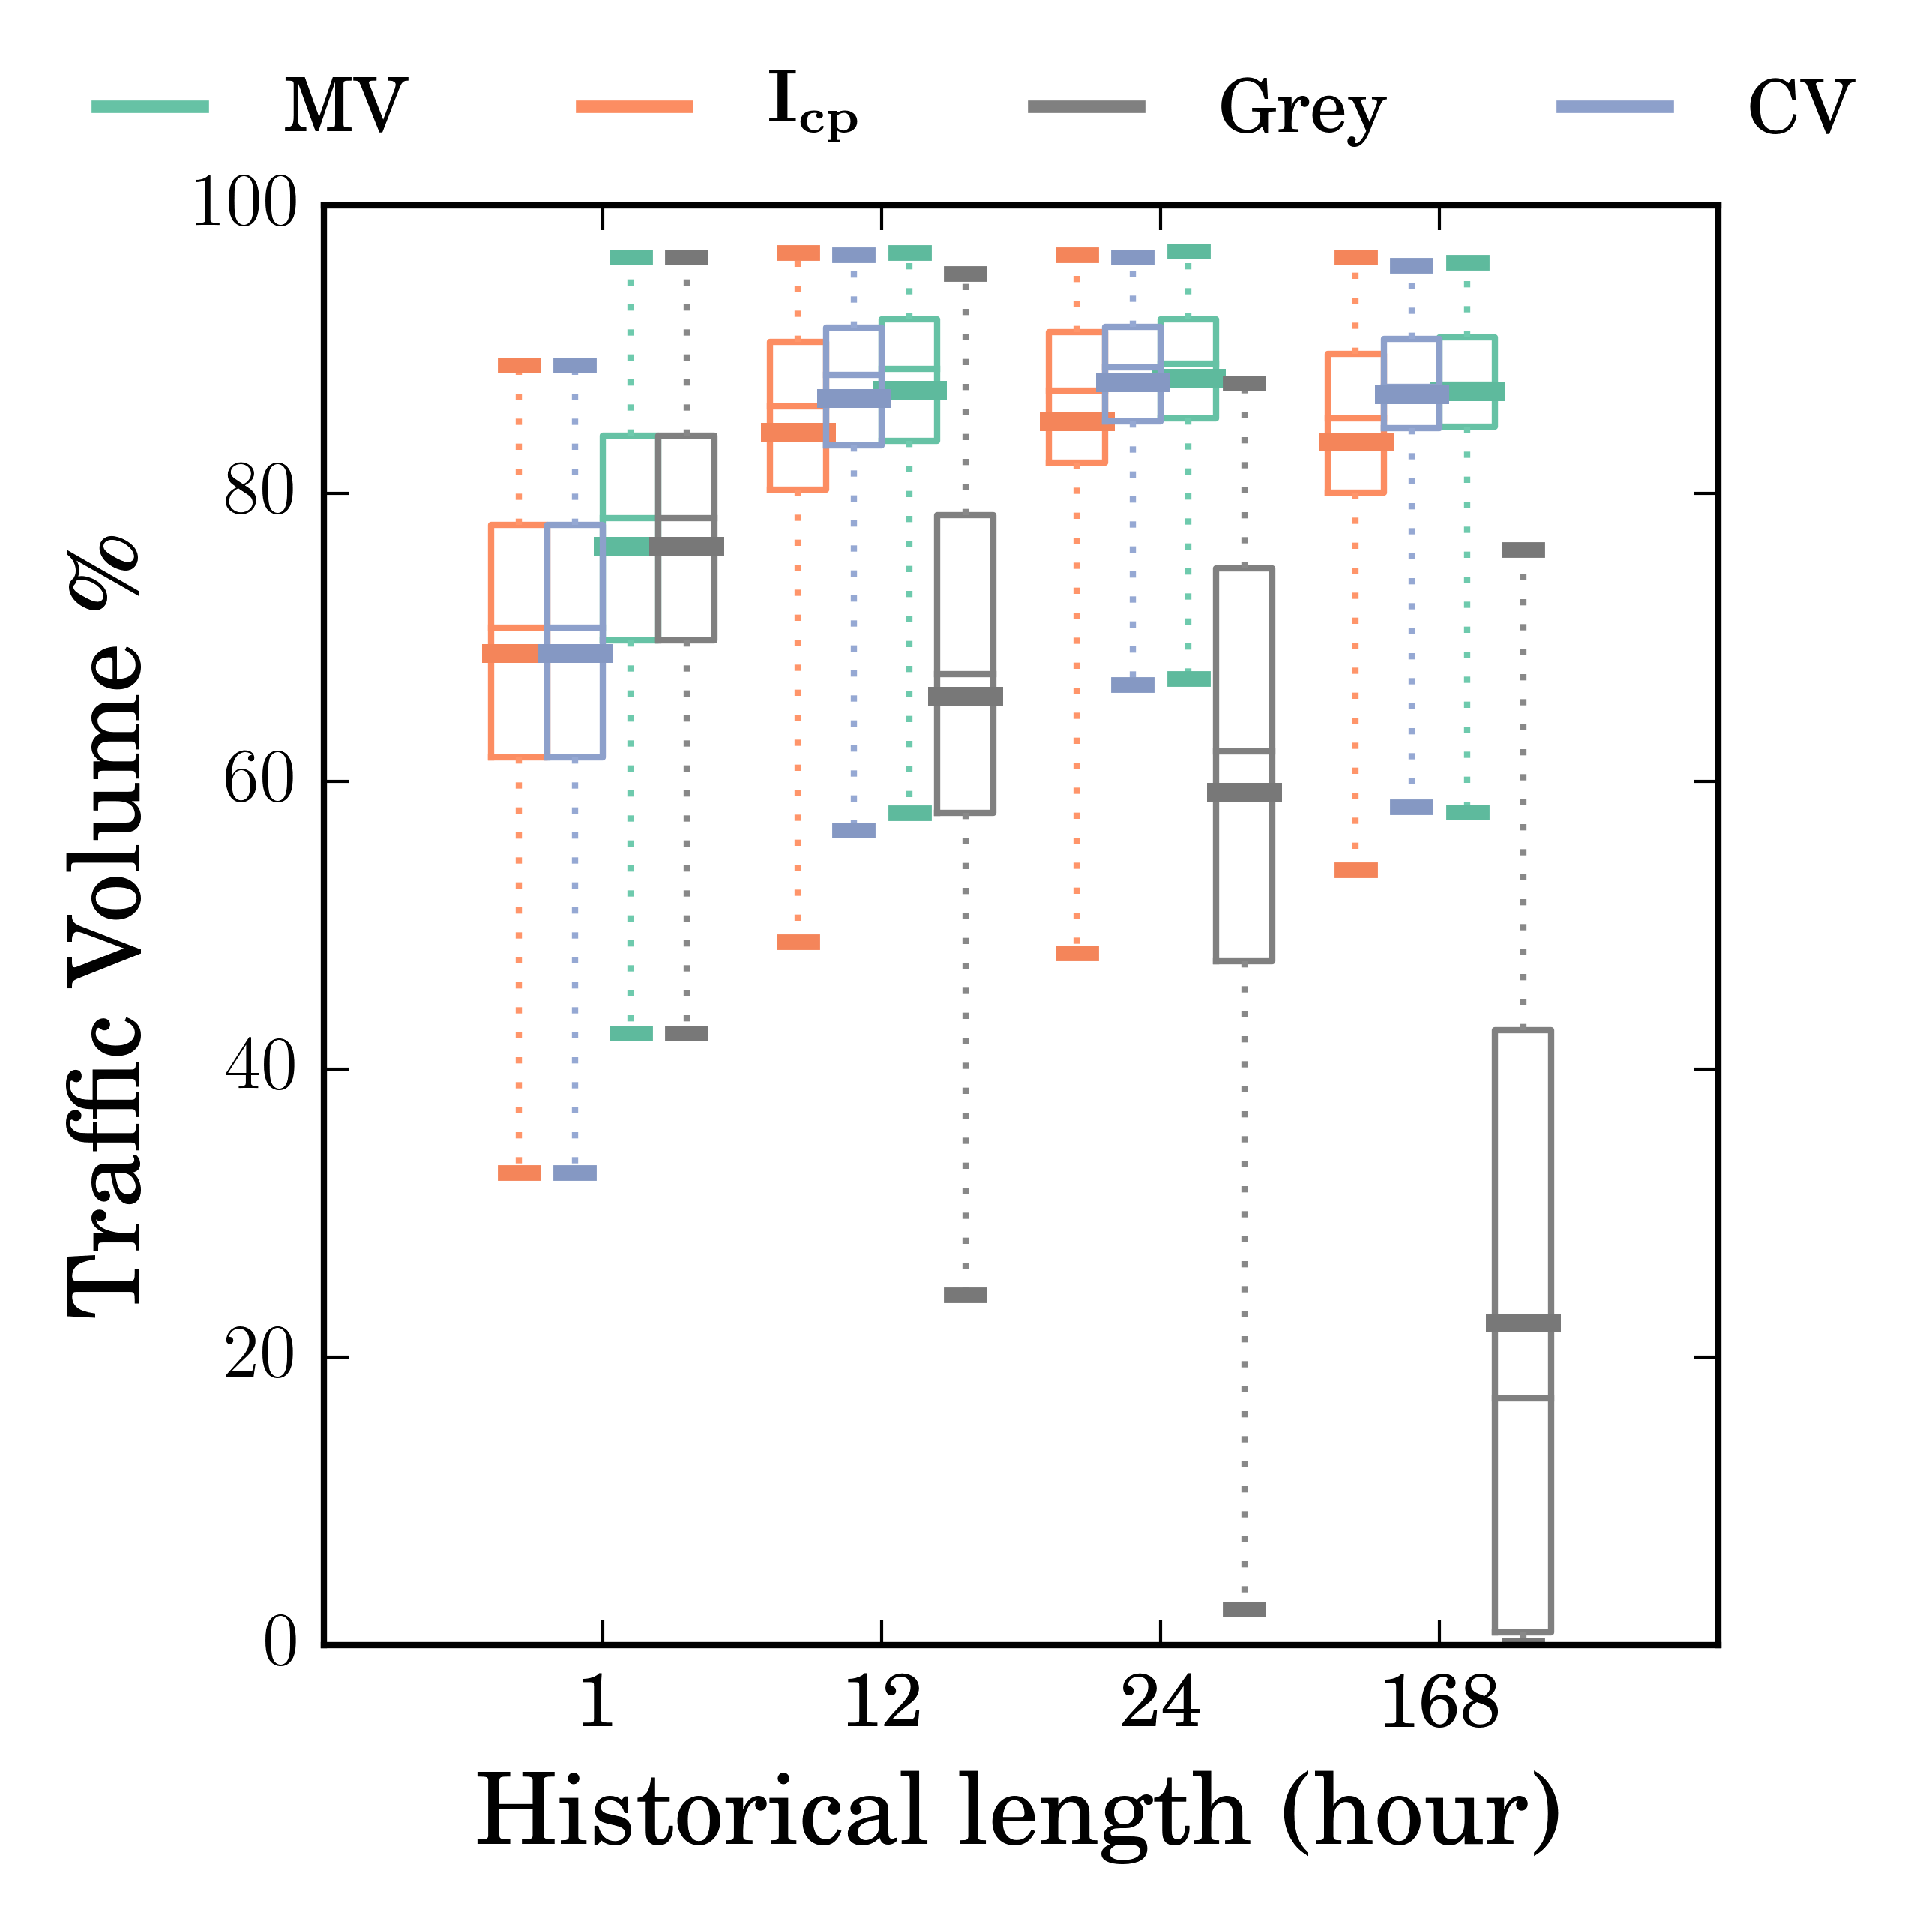
\includegraphics[width=\textwidth]{gfx/chap2/grey_cvg_box_method_compare_fs_si.png}
                \caption{SI}
                \label{fig:cvg_si}
        \end{subfigure}
\caption{(cont.) Hour volume fraction covered by prefixes predictively selected using historical records of different lengths.}
\label{fig:cvg_cont}
\end{figure}

\marginpar{volume coverage}
In evaluating and comparing the performance of these methods, we fixed the selection set size to the maximum \textit{core} size over the week. 
Fig.~\ref{fig:cvg} illustrates the hour volume coverage by the four methods in the form of box-plot, representing the minimum, maximum, 25th and 75th percentile, medium and mean values. 
Among proposed metrics, we find that the $CV$ is very close to $MV$ in terms of volume coverage, proving that it is a good approximation of the later, while being more resource economical.

Basing solely on the last 1 hour records, all methods yield already a mean volume coverage $>80\%$ on SA, SB, SE and SH, which implies a strong continuity on prefix volumes between two consecutive hours. 
On SC and SG, however, using records of last 168 hours, i.e. a week, offers much better minimum volume coverage than shorter records. This is due to the fact that at certain hour, SC and SG undergo a great amount of bursty traffic (as observed previously, e.g. in Table~\ref{tab:bi} and Fig.~\ref{fig:cv_cp}). By increasing the historical length, the selection metrics are able to have better visibility into the past and capture some of these bursty prefixes ---  finally improving the minimum coverage.
This gain in minimum volume coverage by using long historical records can actually be observed on all networks, between 1 hour and 12 hours, also between 12 hour and 24 hour. 
However from 24 hour to 168, this gain doesn't necessary happen on all sites, which is due to the fact that the total volume brought by some highly bursty prefix is diluted by the long time span using $MV$ and $CV$ metrics. In order to capture them, a larger selection set size is need, which inevitably includes more prefixes of few significance.


\begin{figure}
\centering
		\centering
		\begin{subfigure}[b]{0.9\textwidth}
                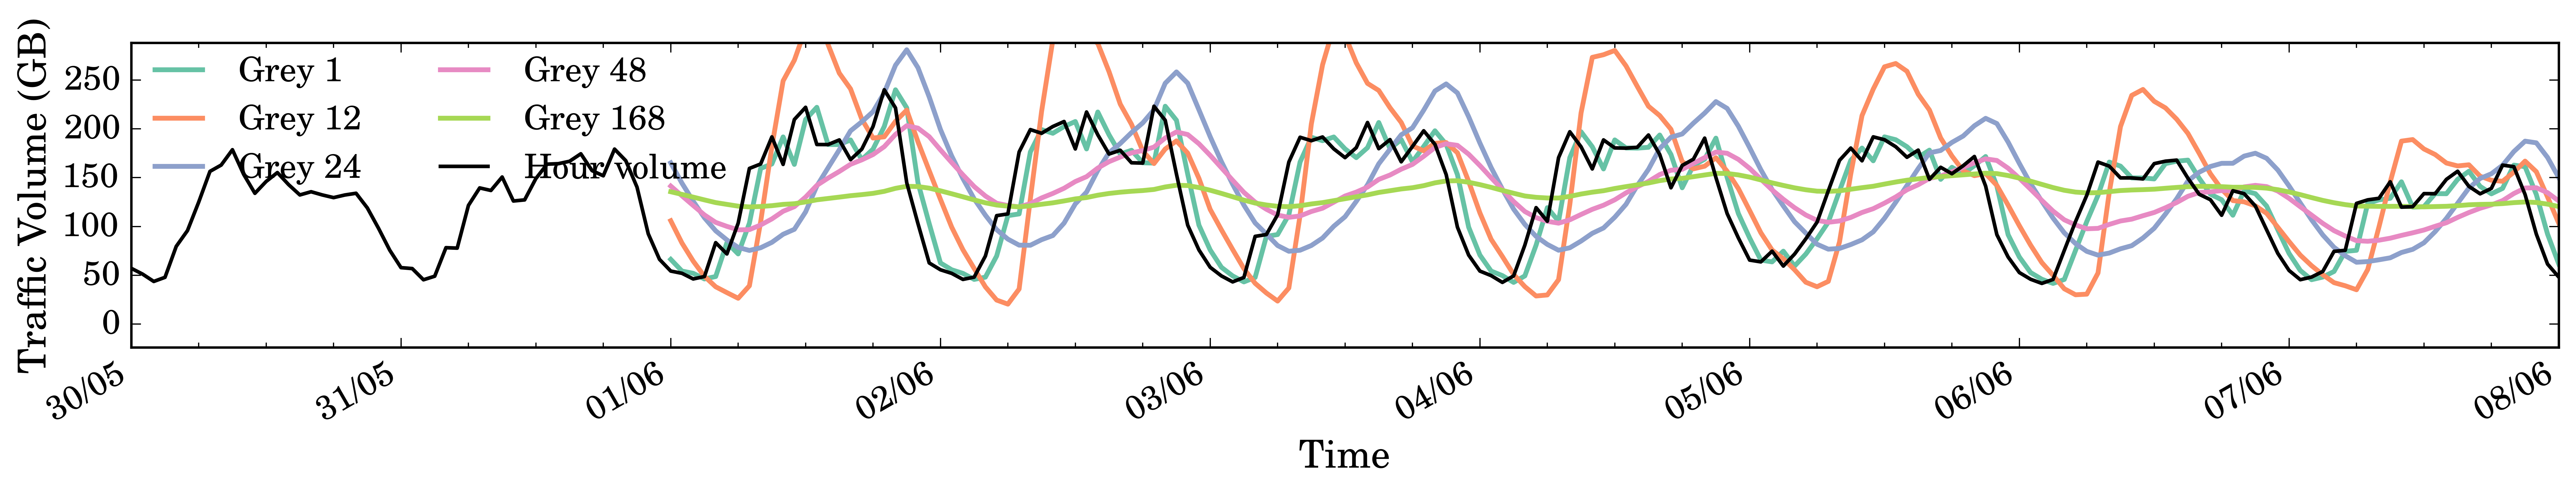
\includegraphics[width=\textwidth]{gfx/chap2/grey_sa.png}
                \caption{SA}
                \label{fig:grey_sa}
        \end{subfigure}
        \begin{subfigure}[b]{0.9\textwidth}
                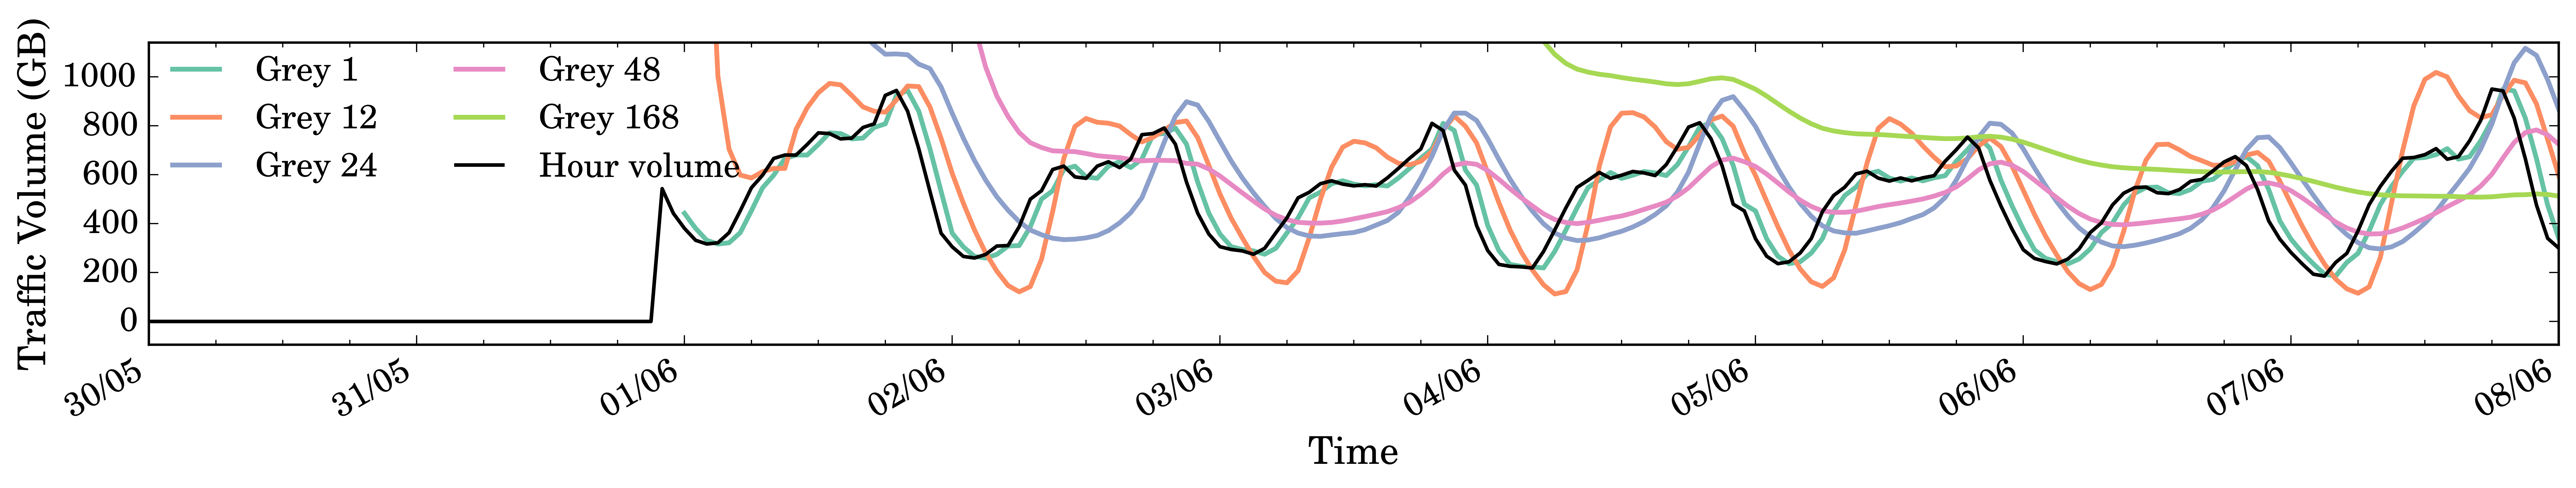
\includegraphics[width=\textwidth]{gfx/chap2/grey_sb.png}
                \caption{SB}
                \label{fig:grey_sb}
        \end{subfigure}
        \begin{subfigure}[b]{0.9\textwidth}
                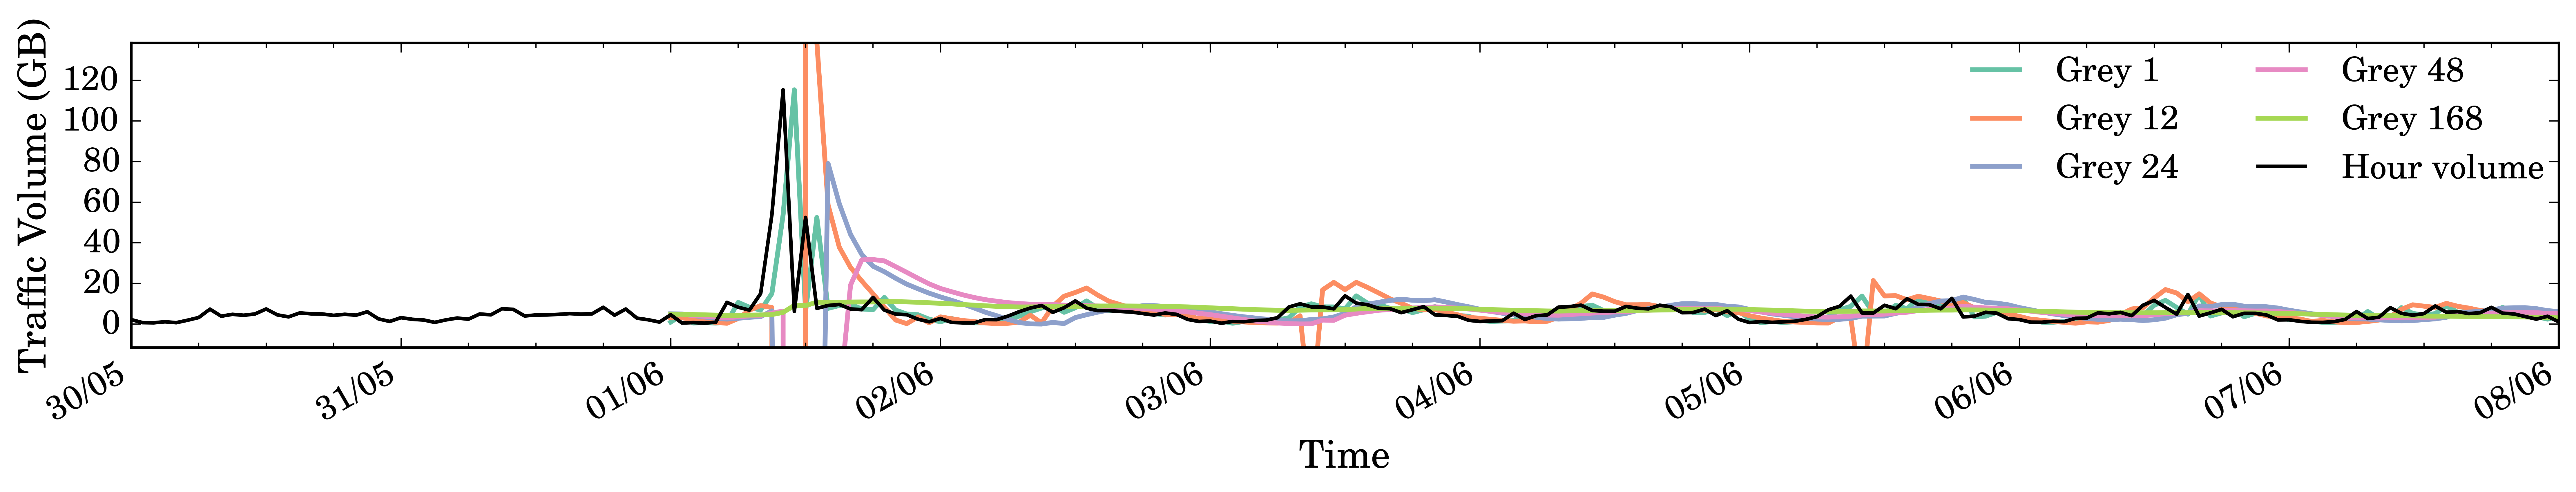
\includegraphics[width=\textwidth]{gfx/chap2/grey_sc.png}
                \caption{SC}
                \label{fig:grey_sc}
        \end{subfigure}
        \begin{subfigure}[b]{0.9\textwidth}
                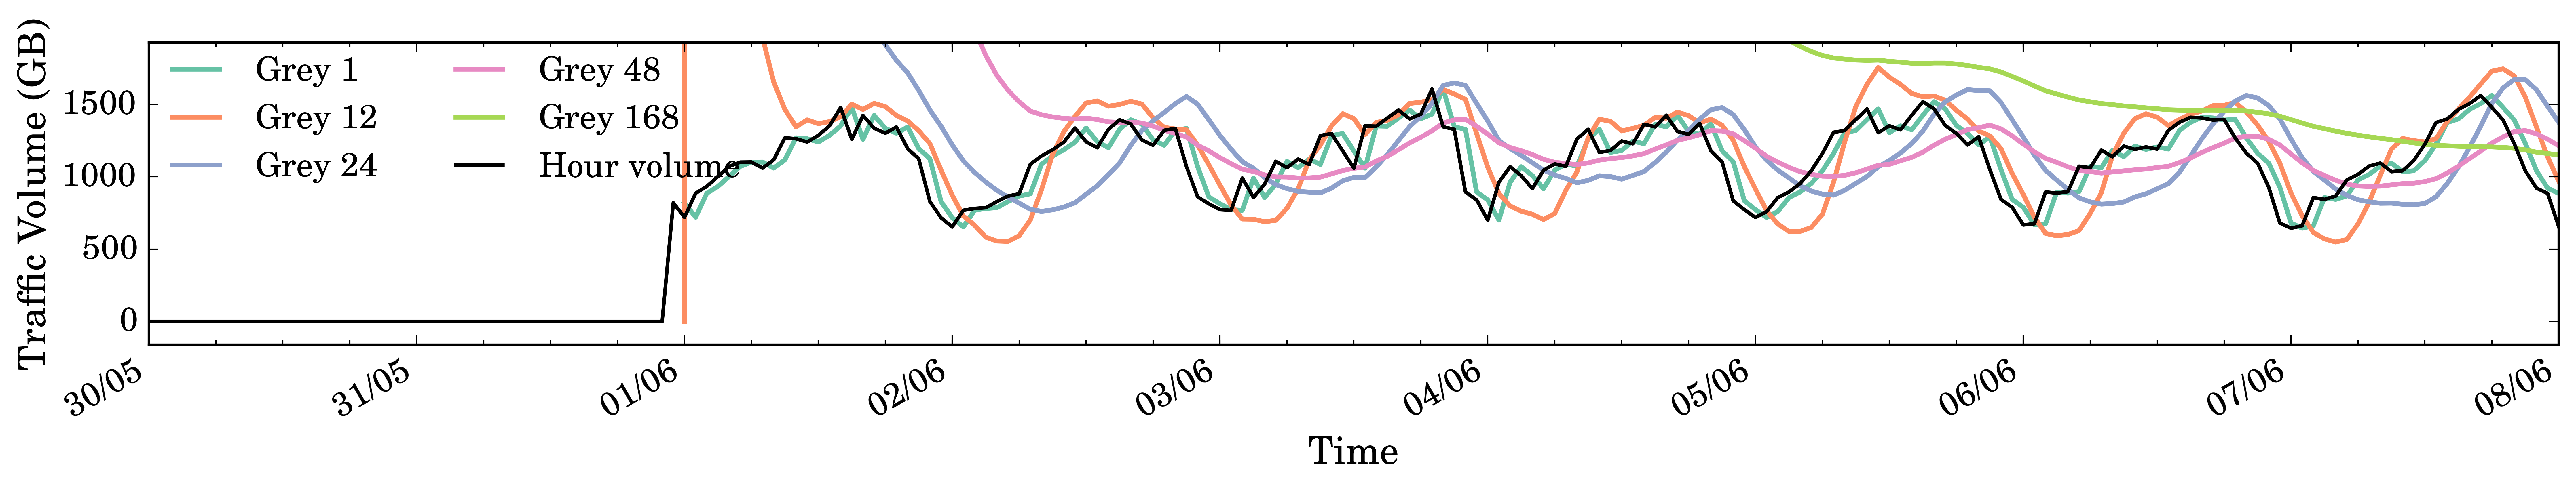
\includegraphics[width=\textwidth]{gfx/chap2/grey_sd.png}
                \caption{SD}
                \label{fig:grey_sd}
        \end{subfigure}
        \begin{subfigure}[b]{0.9\textwidth}
                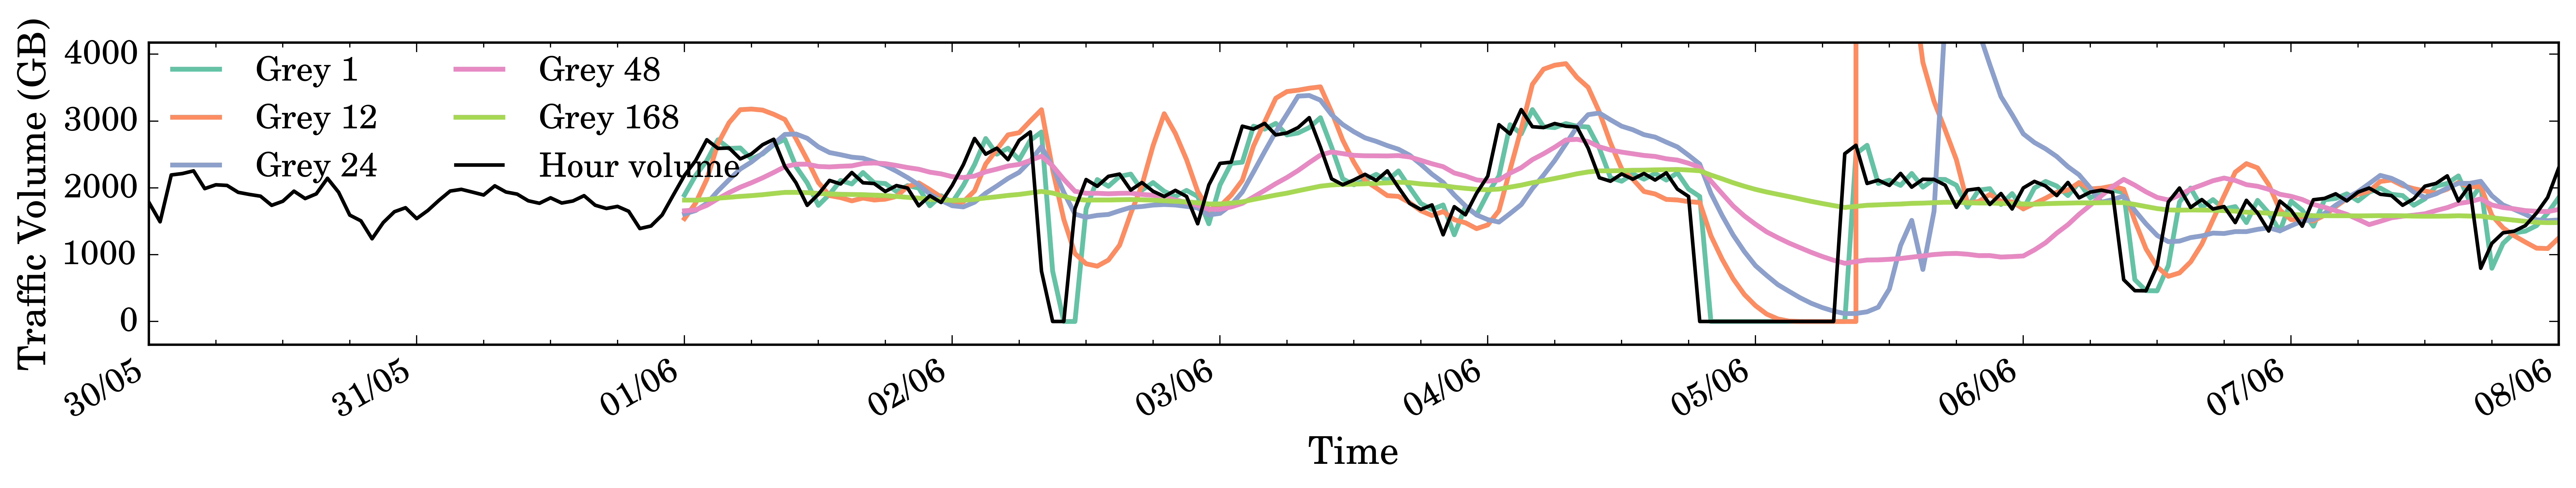
\includegraphics[width=\textwidth]{gfx/chap2/grey_se.png}
                \caption{SE}
                \label{fig:grey_se}
        \end{subfigure}
        \begin{subfigure}[b]{0.9\textwidth}
                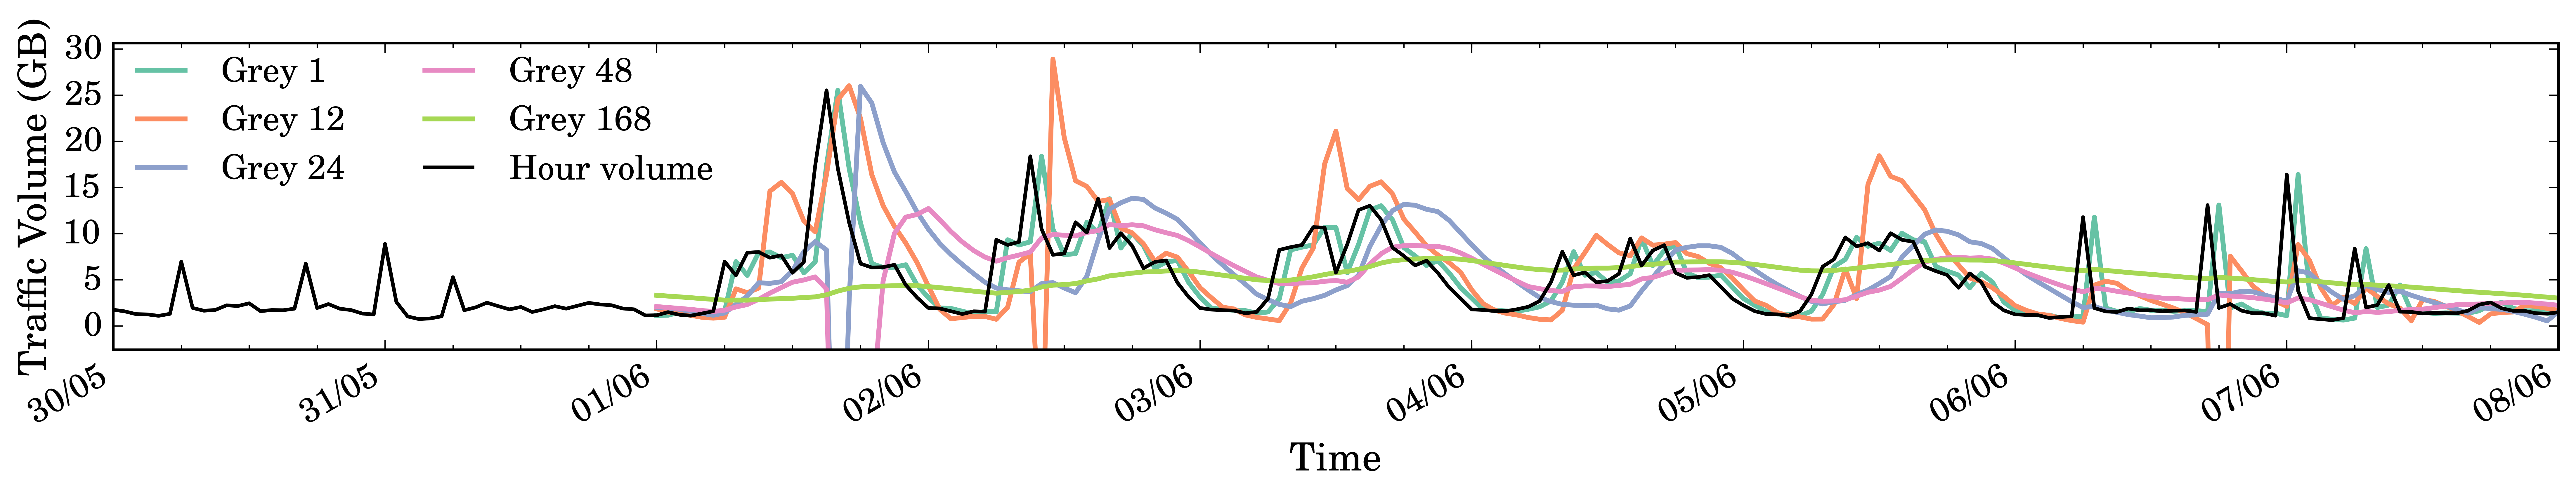
\includegraphics[width=\textwidth]{gfx/chap2/grey_sf.png}
                \caption{SF}
                \label{fig:grey_sf}
        \end{subfigure}
        \begin{subfigure}[b]{0.9\textwidth}
                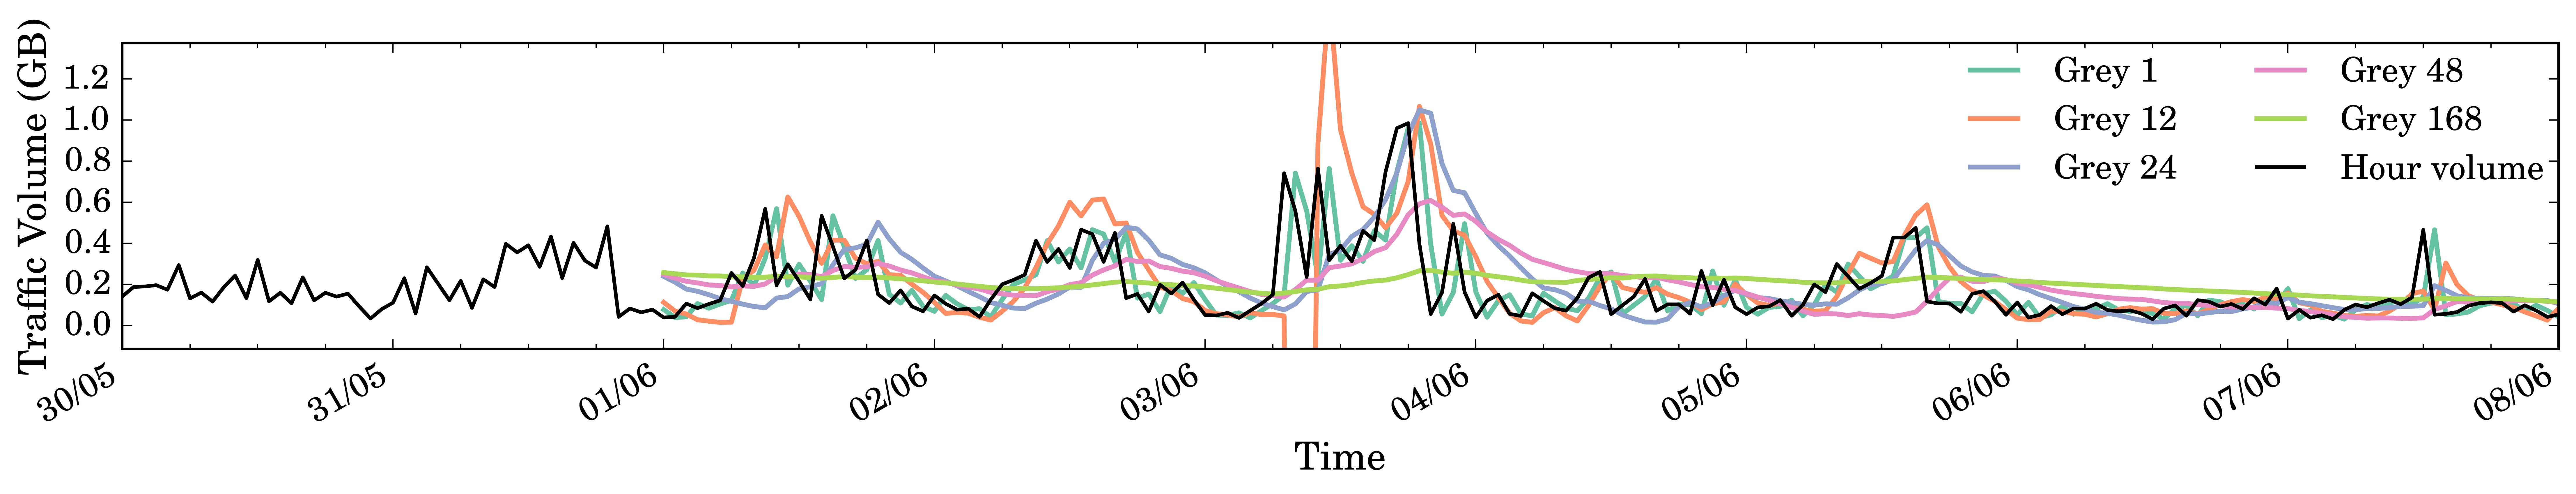
\includegraphics[width=\textwidth]{gfx/chap2/grey_sg.png}
                \caption{SG}
                \label{fig:grey_sg}
        \end{subfigure}
        \begin{subfigure}[b]{0.9\textwidth}
                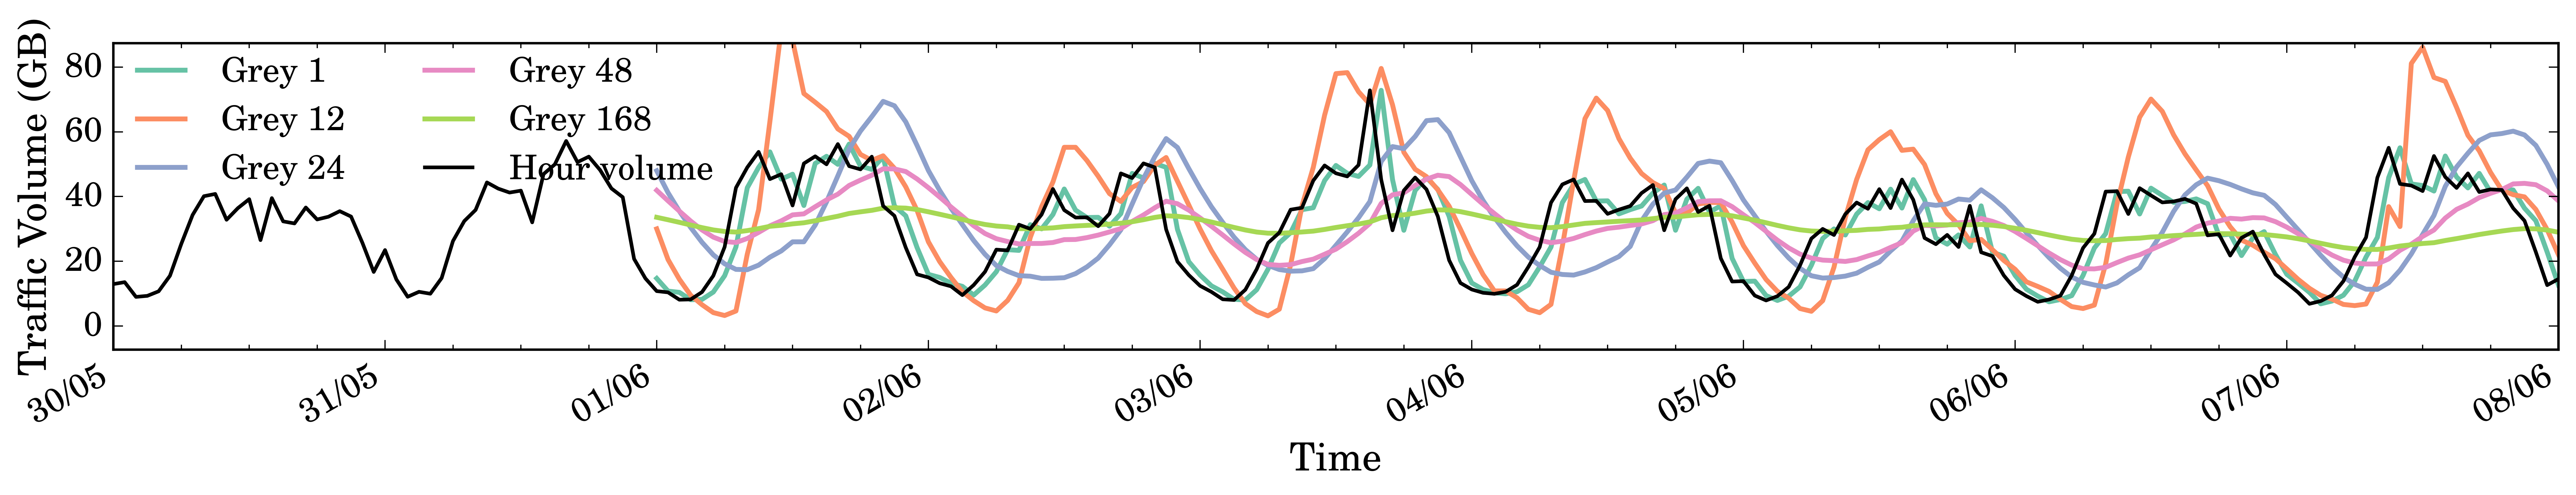
\includegraphics[width=\textwidth]{gfx/chap2/grey_sh.png}
                \caption{SH}
                \label{fig:grey_sh}
        \end{subfigure}
        \begin{subfigure}[b]{0.9\textwidth}
                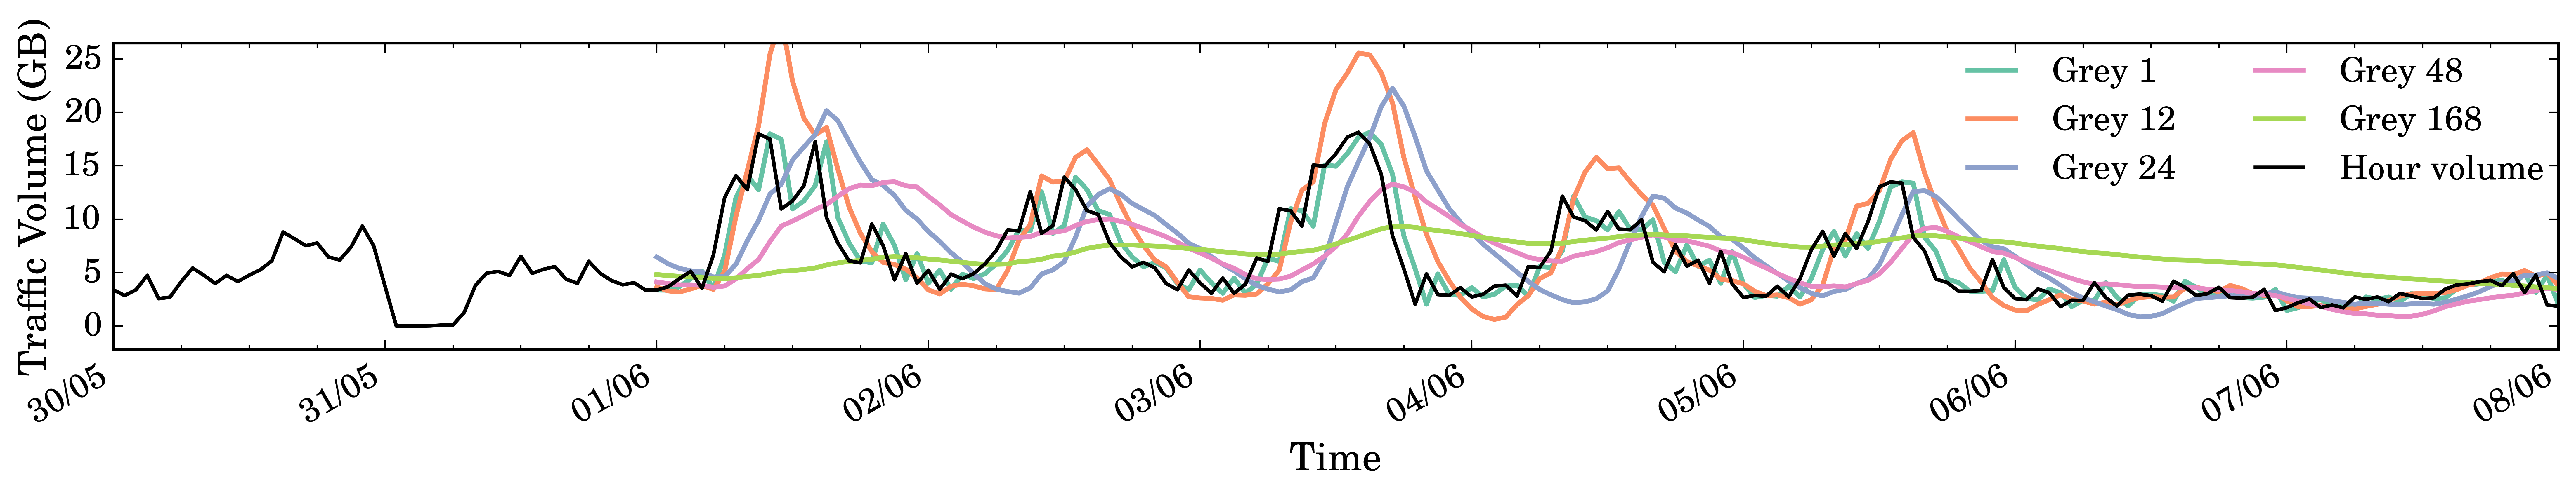
\includegraphics[width=\textwidth]{gfx/chap2/grey_si.png}
                \caption{SI}
                \label{fig:grey_si}
        \end{subfigure}
\caption{Predict total hour volume using $GM(1,1)$ with different historical record lengths for the week starting from June 1st, 2015.}
\label{fig:grey}
\end{figure}

\marginpar{Why grey model performs poorly?}
On the other hand, the hour volume coverage by grey model drops as we increase the historical records length and is in general much worse than the metrics proposed in this work. 
In order to understand the underlying reason, we used $GM(1,1)$ model described above to dynamically predict the total hour volume of all prefixes, which is normally much more regular and smoother than the volume series of individual prefixes, Fig.~\ref{fig:grey}.

\marginpar{overreact to sudden value change.}
For site SB and SD, we miss the hour volume data for the week starting from May 25th. 
$GM(1,1)$ model using records of last $168$ suffer a lot from  data missing and converge extremely slow to values in reasonable range. 
However, such sudden change in value is not unexpected, since bursty prefixes can bring huge amount of traffic within in a short duration and then remain silent over days. Such prefixes are commonly seen on SC, SF, SG judging from their burstiness index in Table~\ref{tab:bi}.
This explains why grey model leads to fairly low volume coverage in Fig.~\ref{fig:cvg_sc}. 

\marginpar{delayed response to value change}
Furthermore, in Fig.~\ref{fig:grey_sb}, Fig.~\ref{fig:grey_sc} and as well in others, we can see that grey model reacts to volume variations in a delayed manner. Longer the historical records length is, more obvious and longer grey model delays the variations of actual trace.  
This behavior could be fatal in the presence of bursty prefixes.
We can observe considerably large pikes in both directions several hours after the volume burst in Fig.~\ref{fig:grey_sc}, which might greatly disturb the prefix selection during those periods and consequently give rise to low volume coverage.

Compared to grey model, metrics proposed in our work do not directly predict hour volumes of each prefix but rather are indirect measures of prefix volume importance. And analysis in Section~\ref{sec:dyna} showed that the overall coverage using these metrics are guaranteed by the traffic character itself.

\begin{figure}
\centering
		\centering
        \begin{subfigure}[b]{0.48\textwidth}
                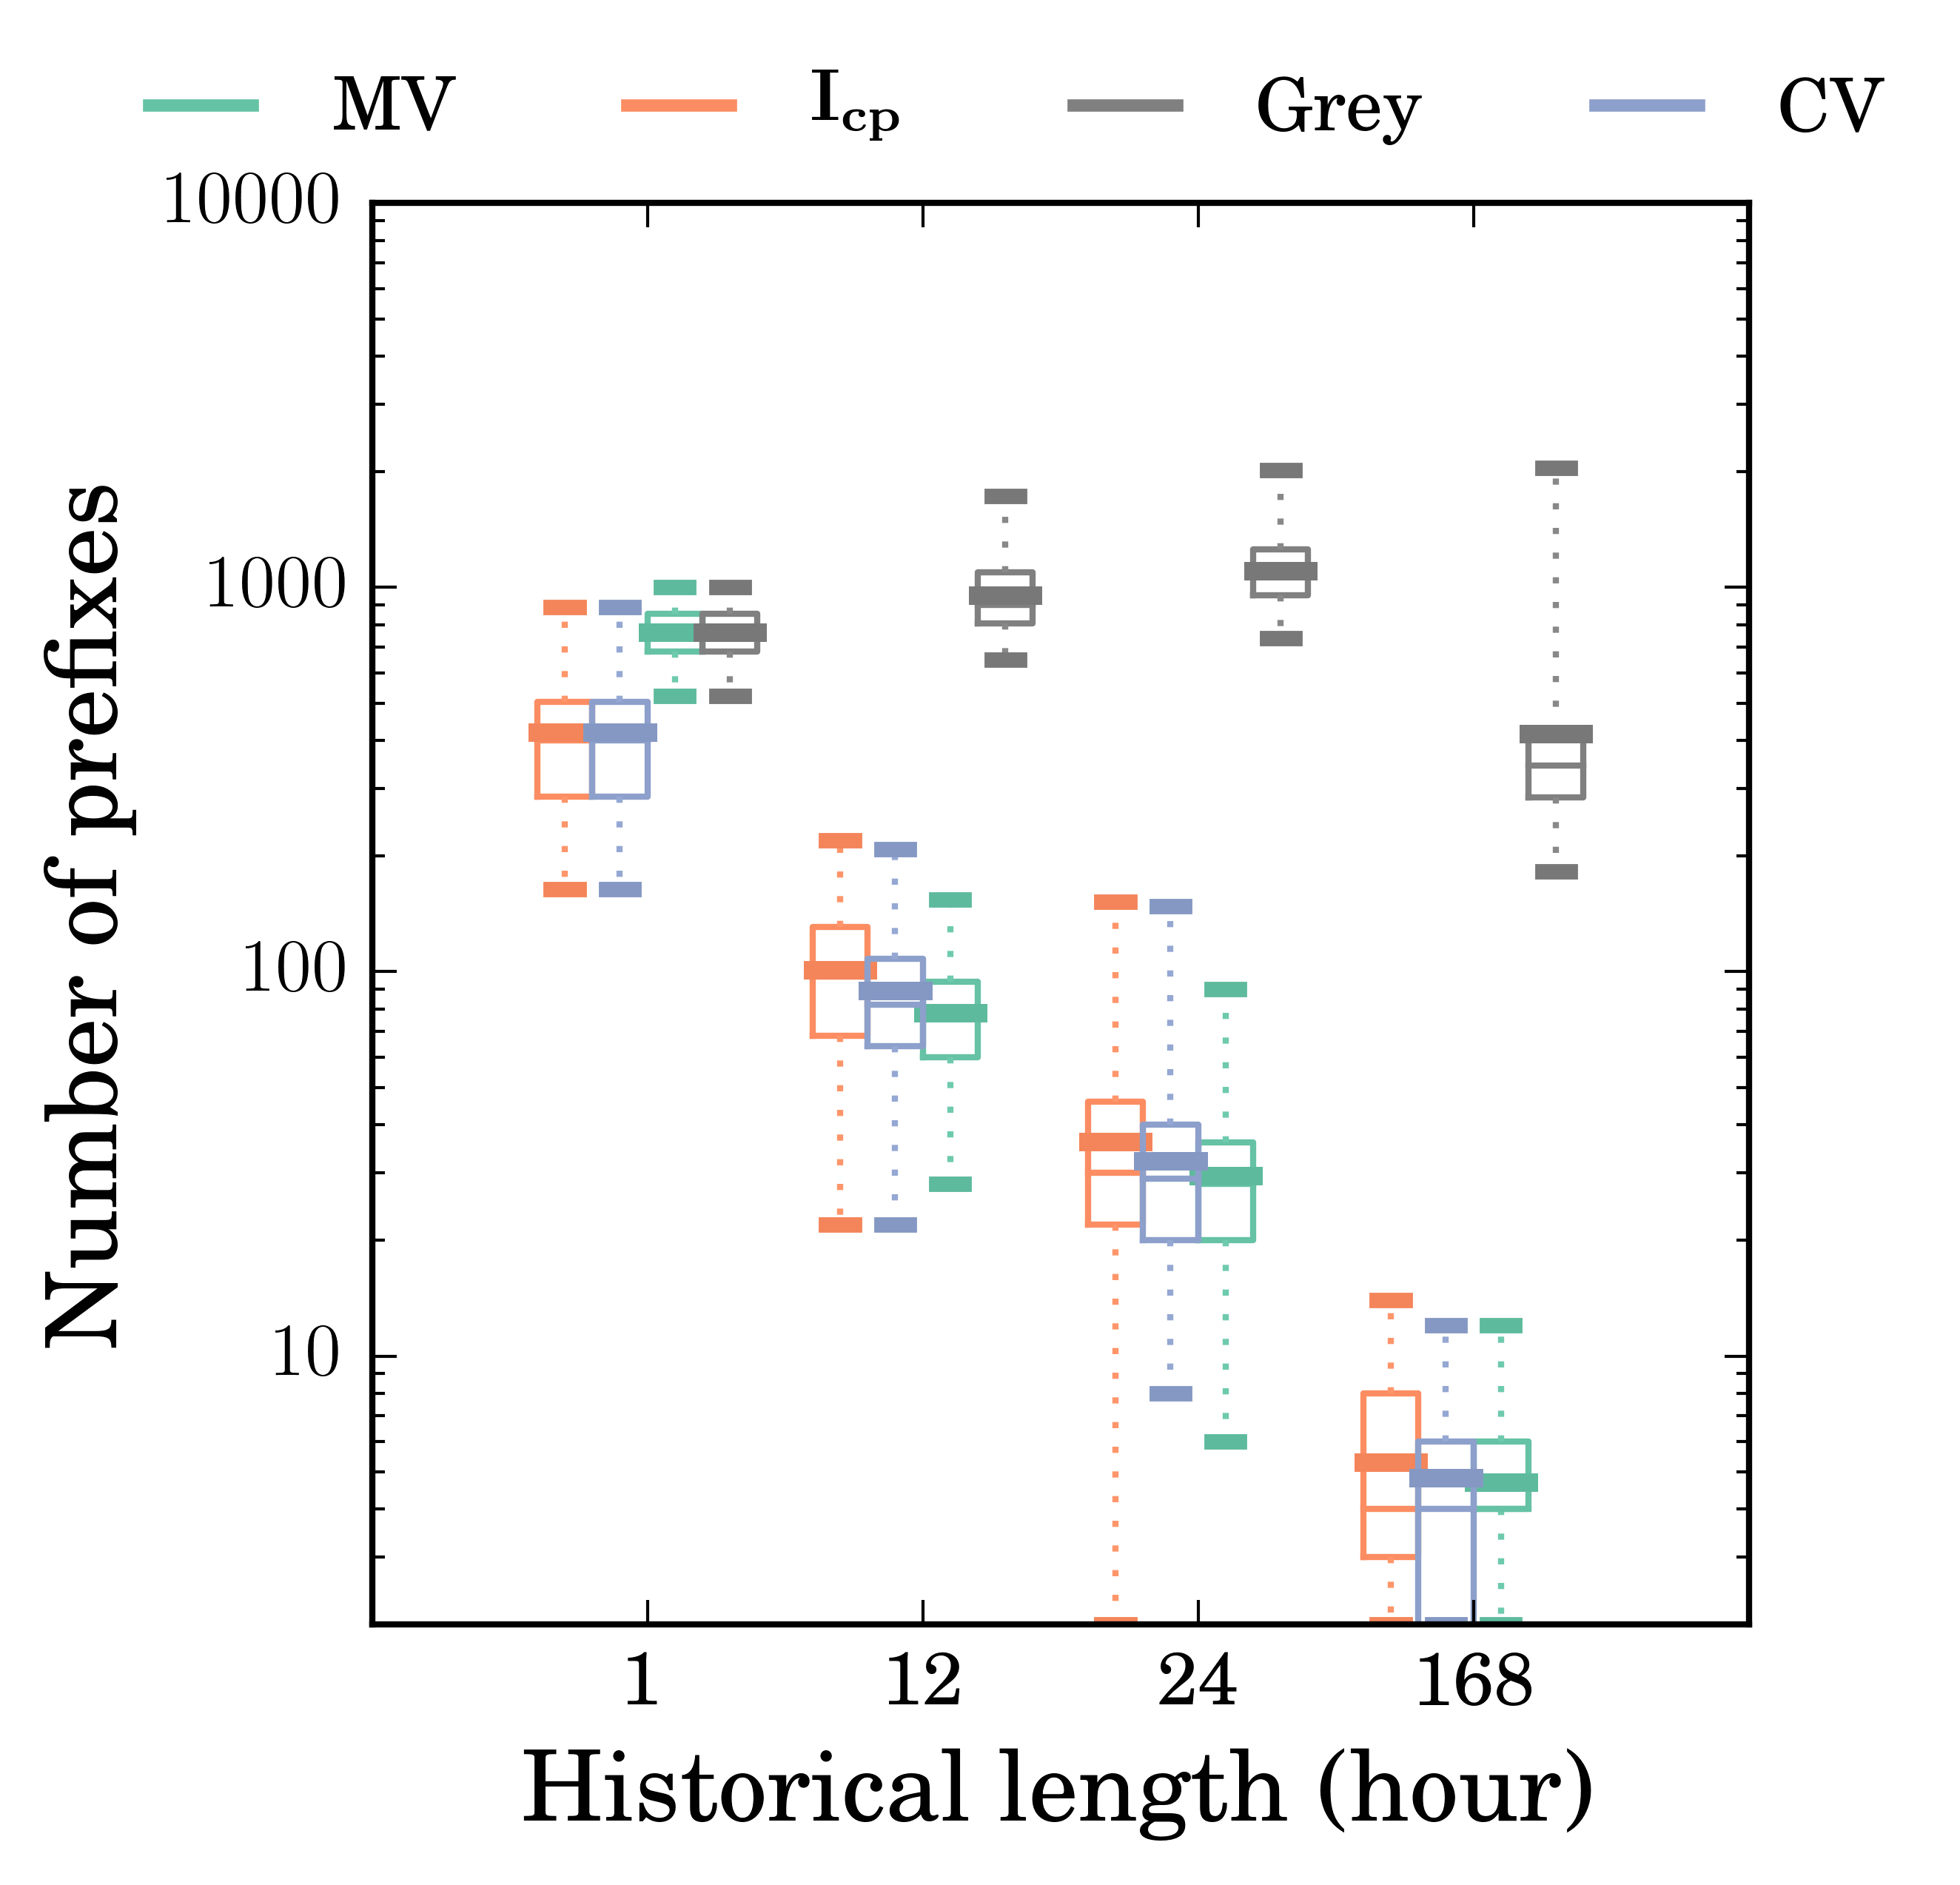
\includegraphics[width=\textwidth]{gfx/chap2/grey_churn_box_method_compare_fs_sa.png}
                \caption{SA}
                \label{fig:churn_sa}
        \end{subfigure}
        \begin{subfigure}[b]{0.48\textwidth}
                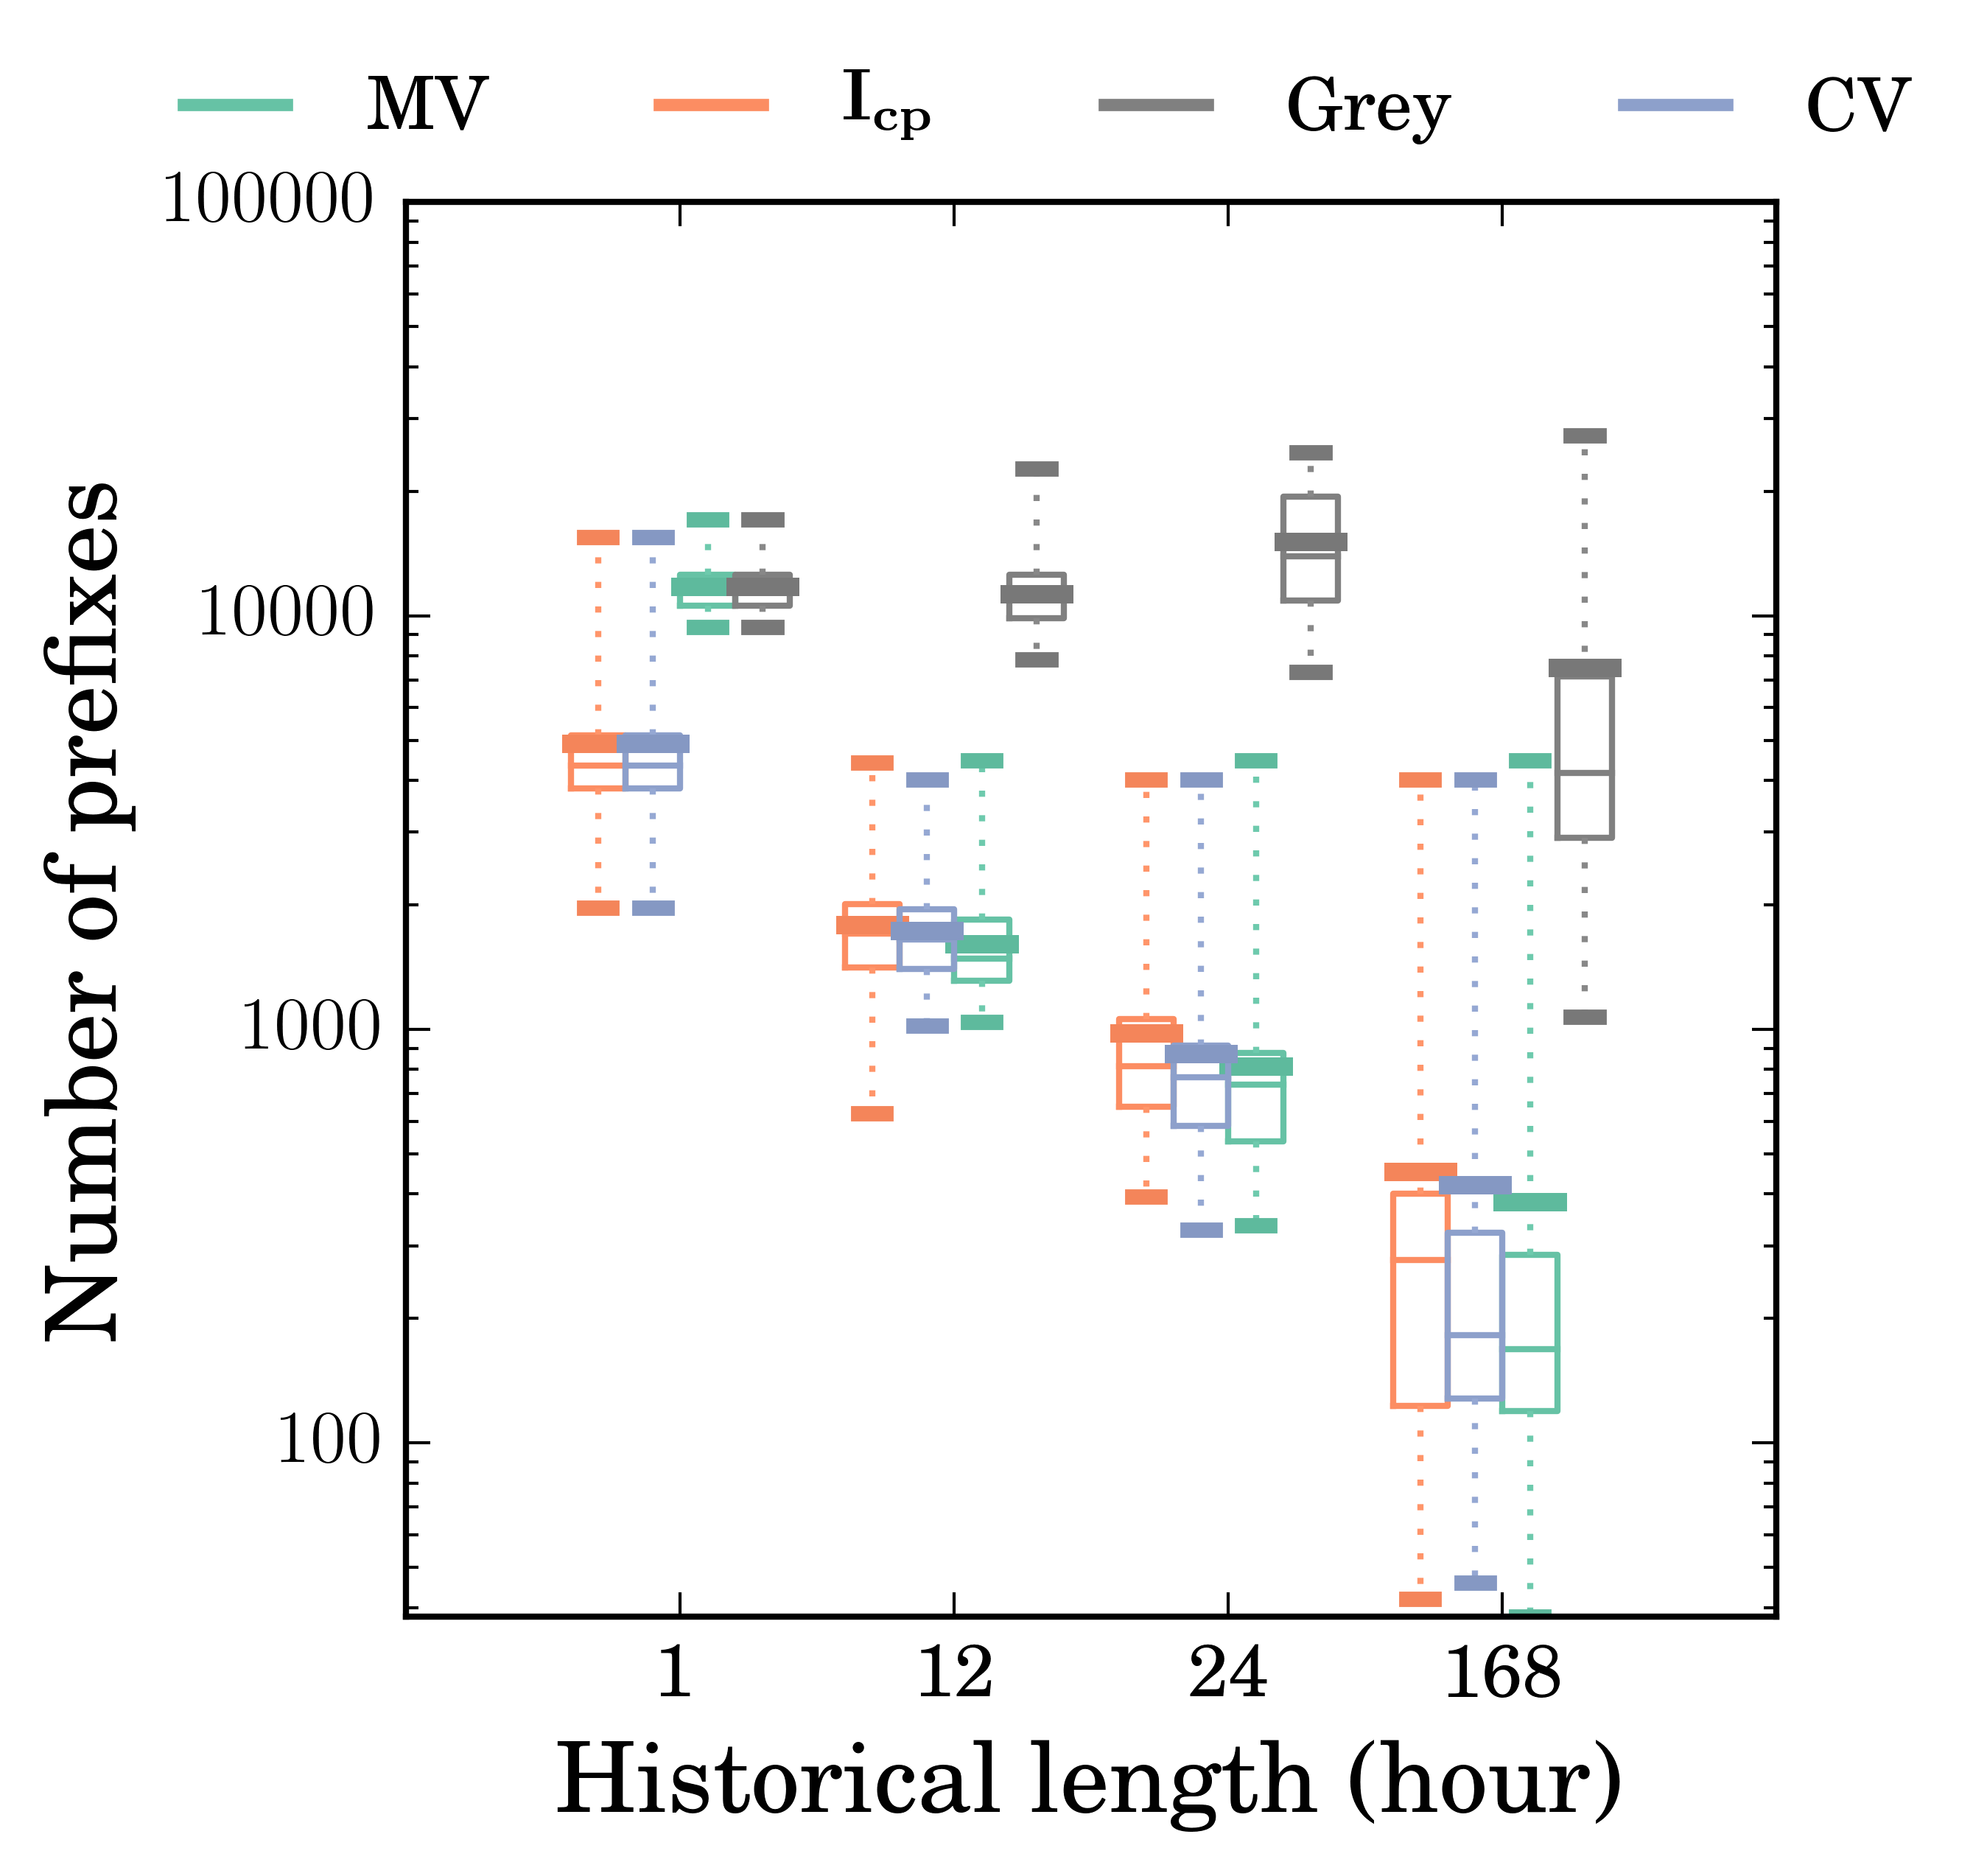
\includegraphics[width=\textwidth]{gfx/chap2/grey_churn_box_method_compare_fs_sb.png}
                \caption{SB}
                \label{fig:churn_sb}
        \end{subfigure}
        \begin{subfigure}[b]{0.48\textwidth}
                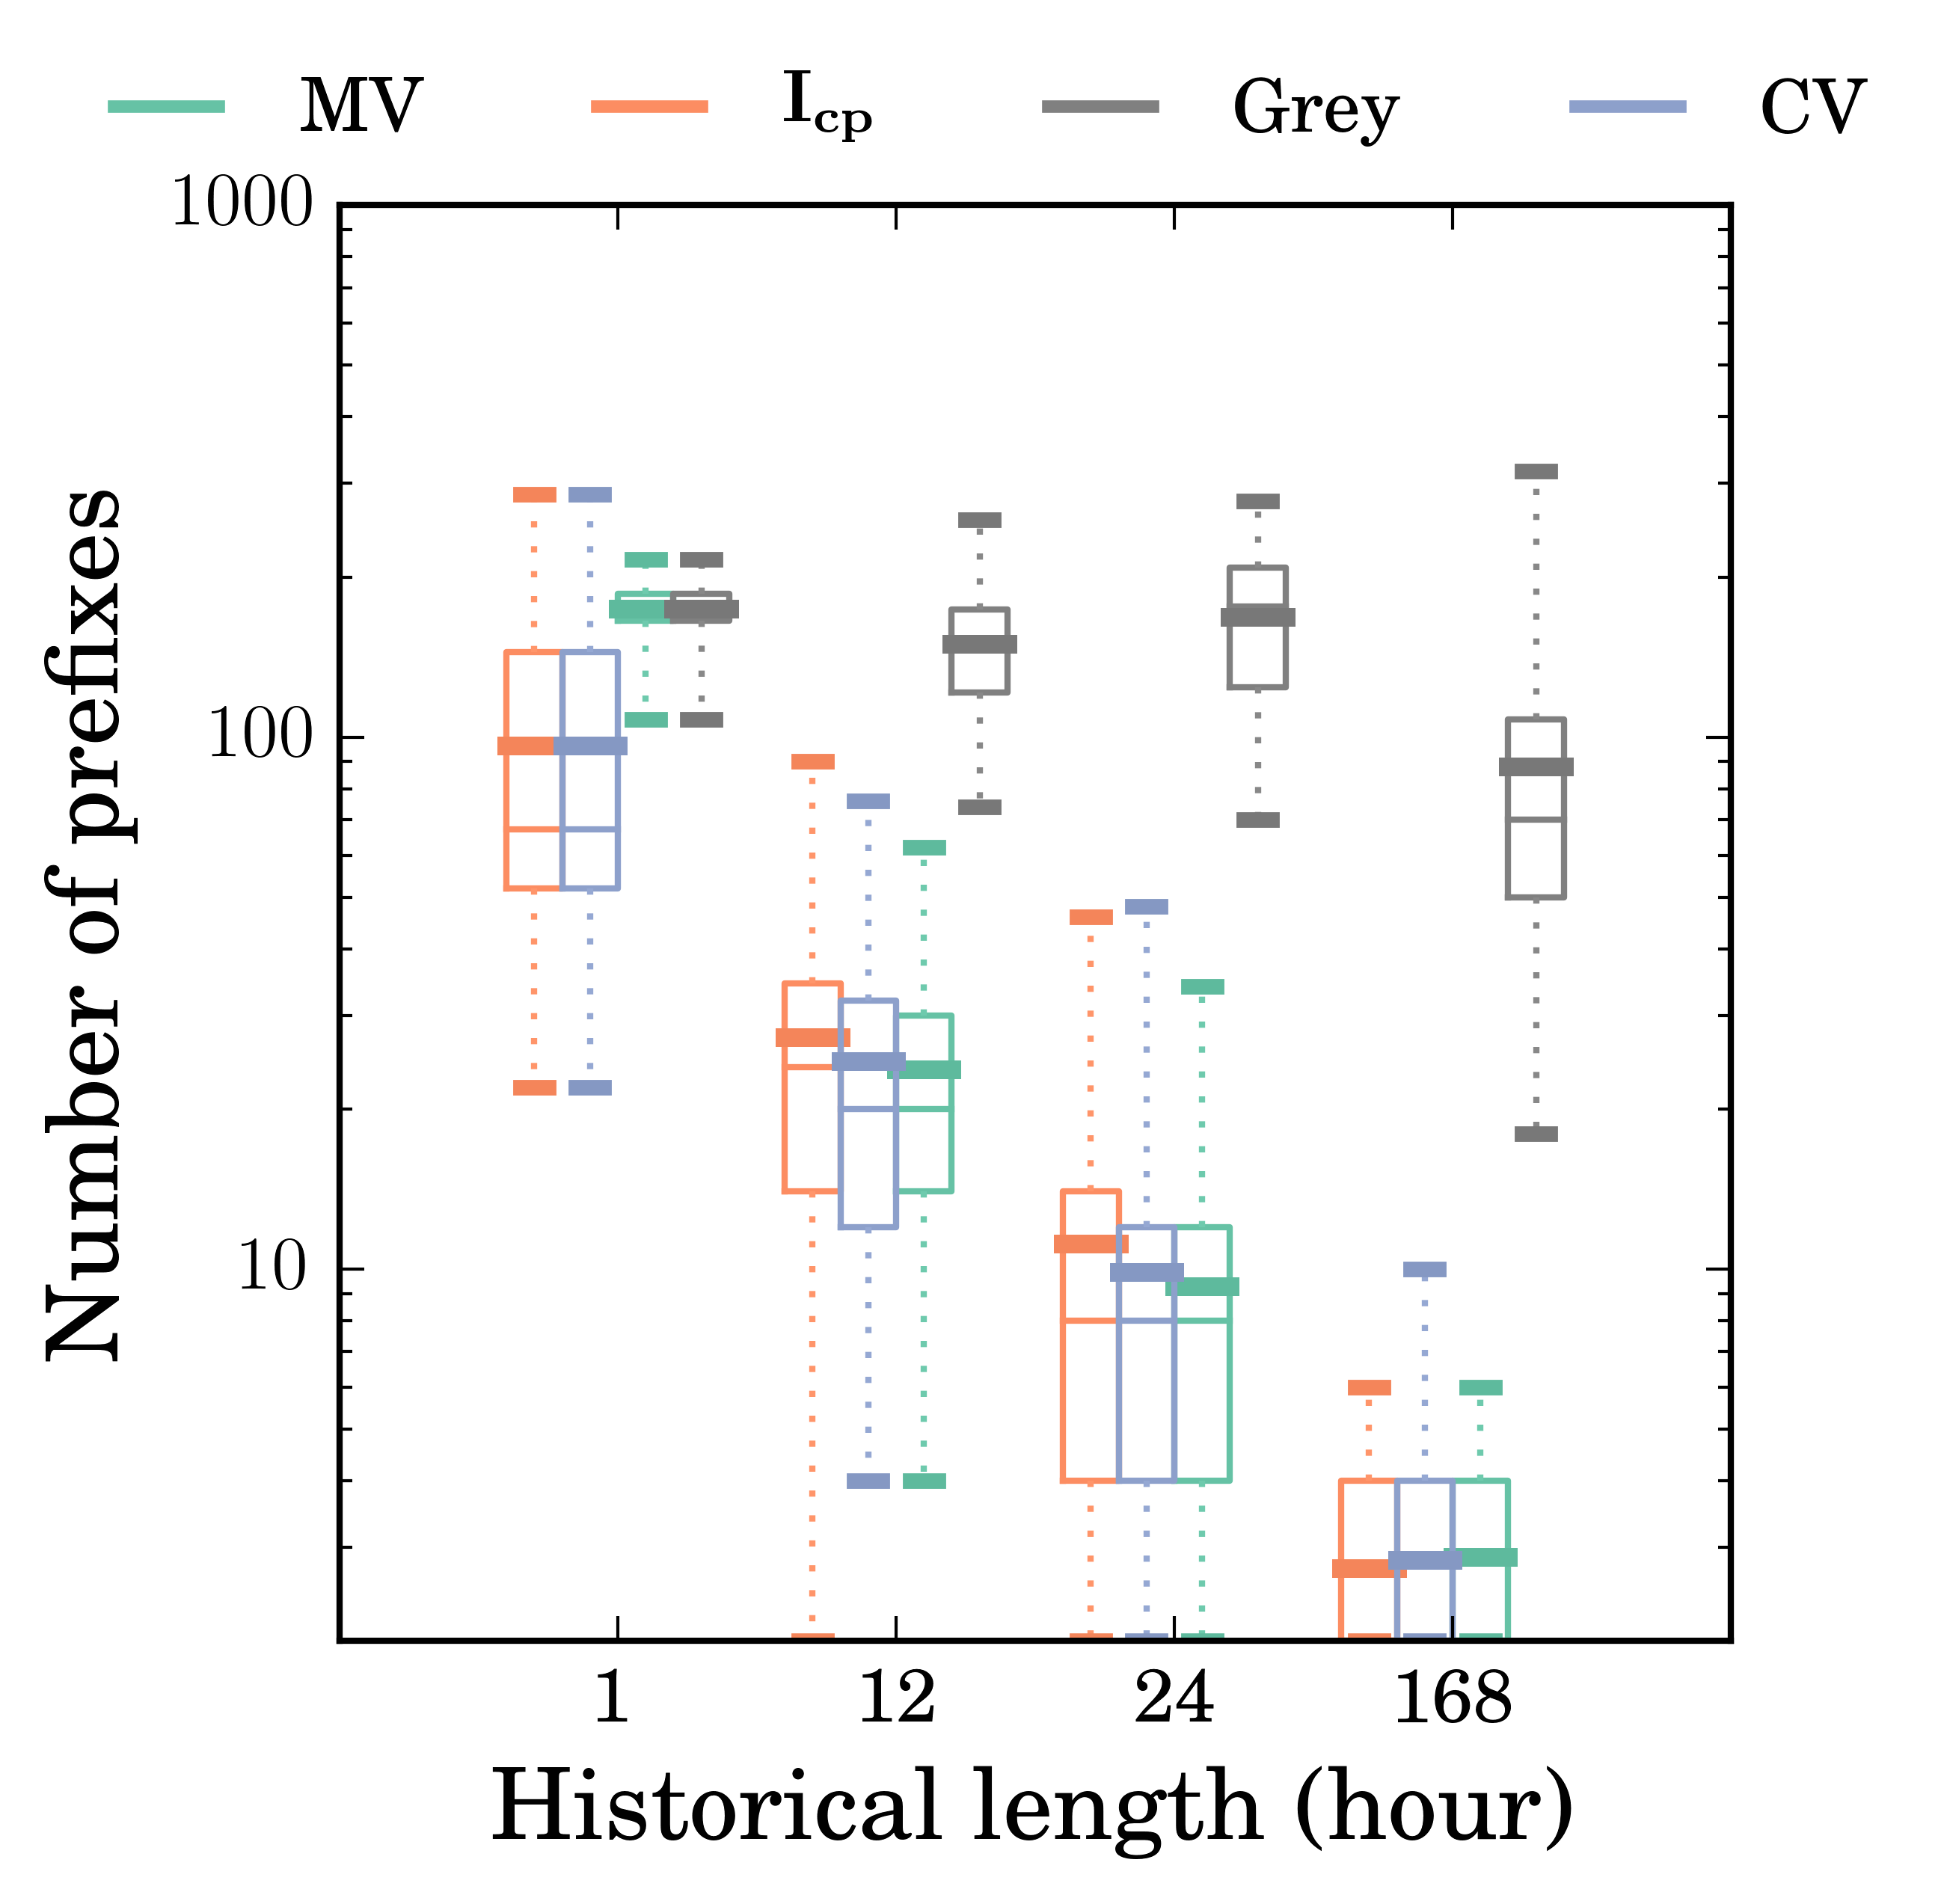
\includegraphics[width=\textwidth]{gfx/chap2/grey_churn_box_method_compare_fs_sc.png}
                \caption{SC}
                \label{fig:churn_sc}
        \end{subfigure}
        \begin{subfigure}[b]{0.48\textwidth}
                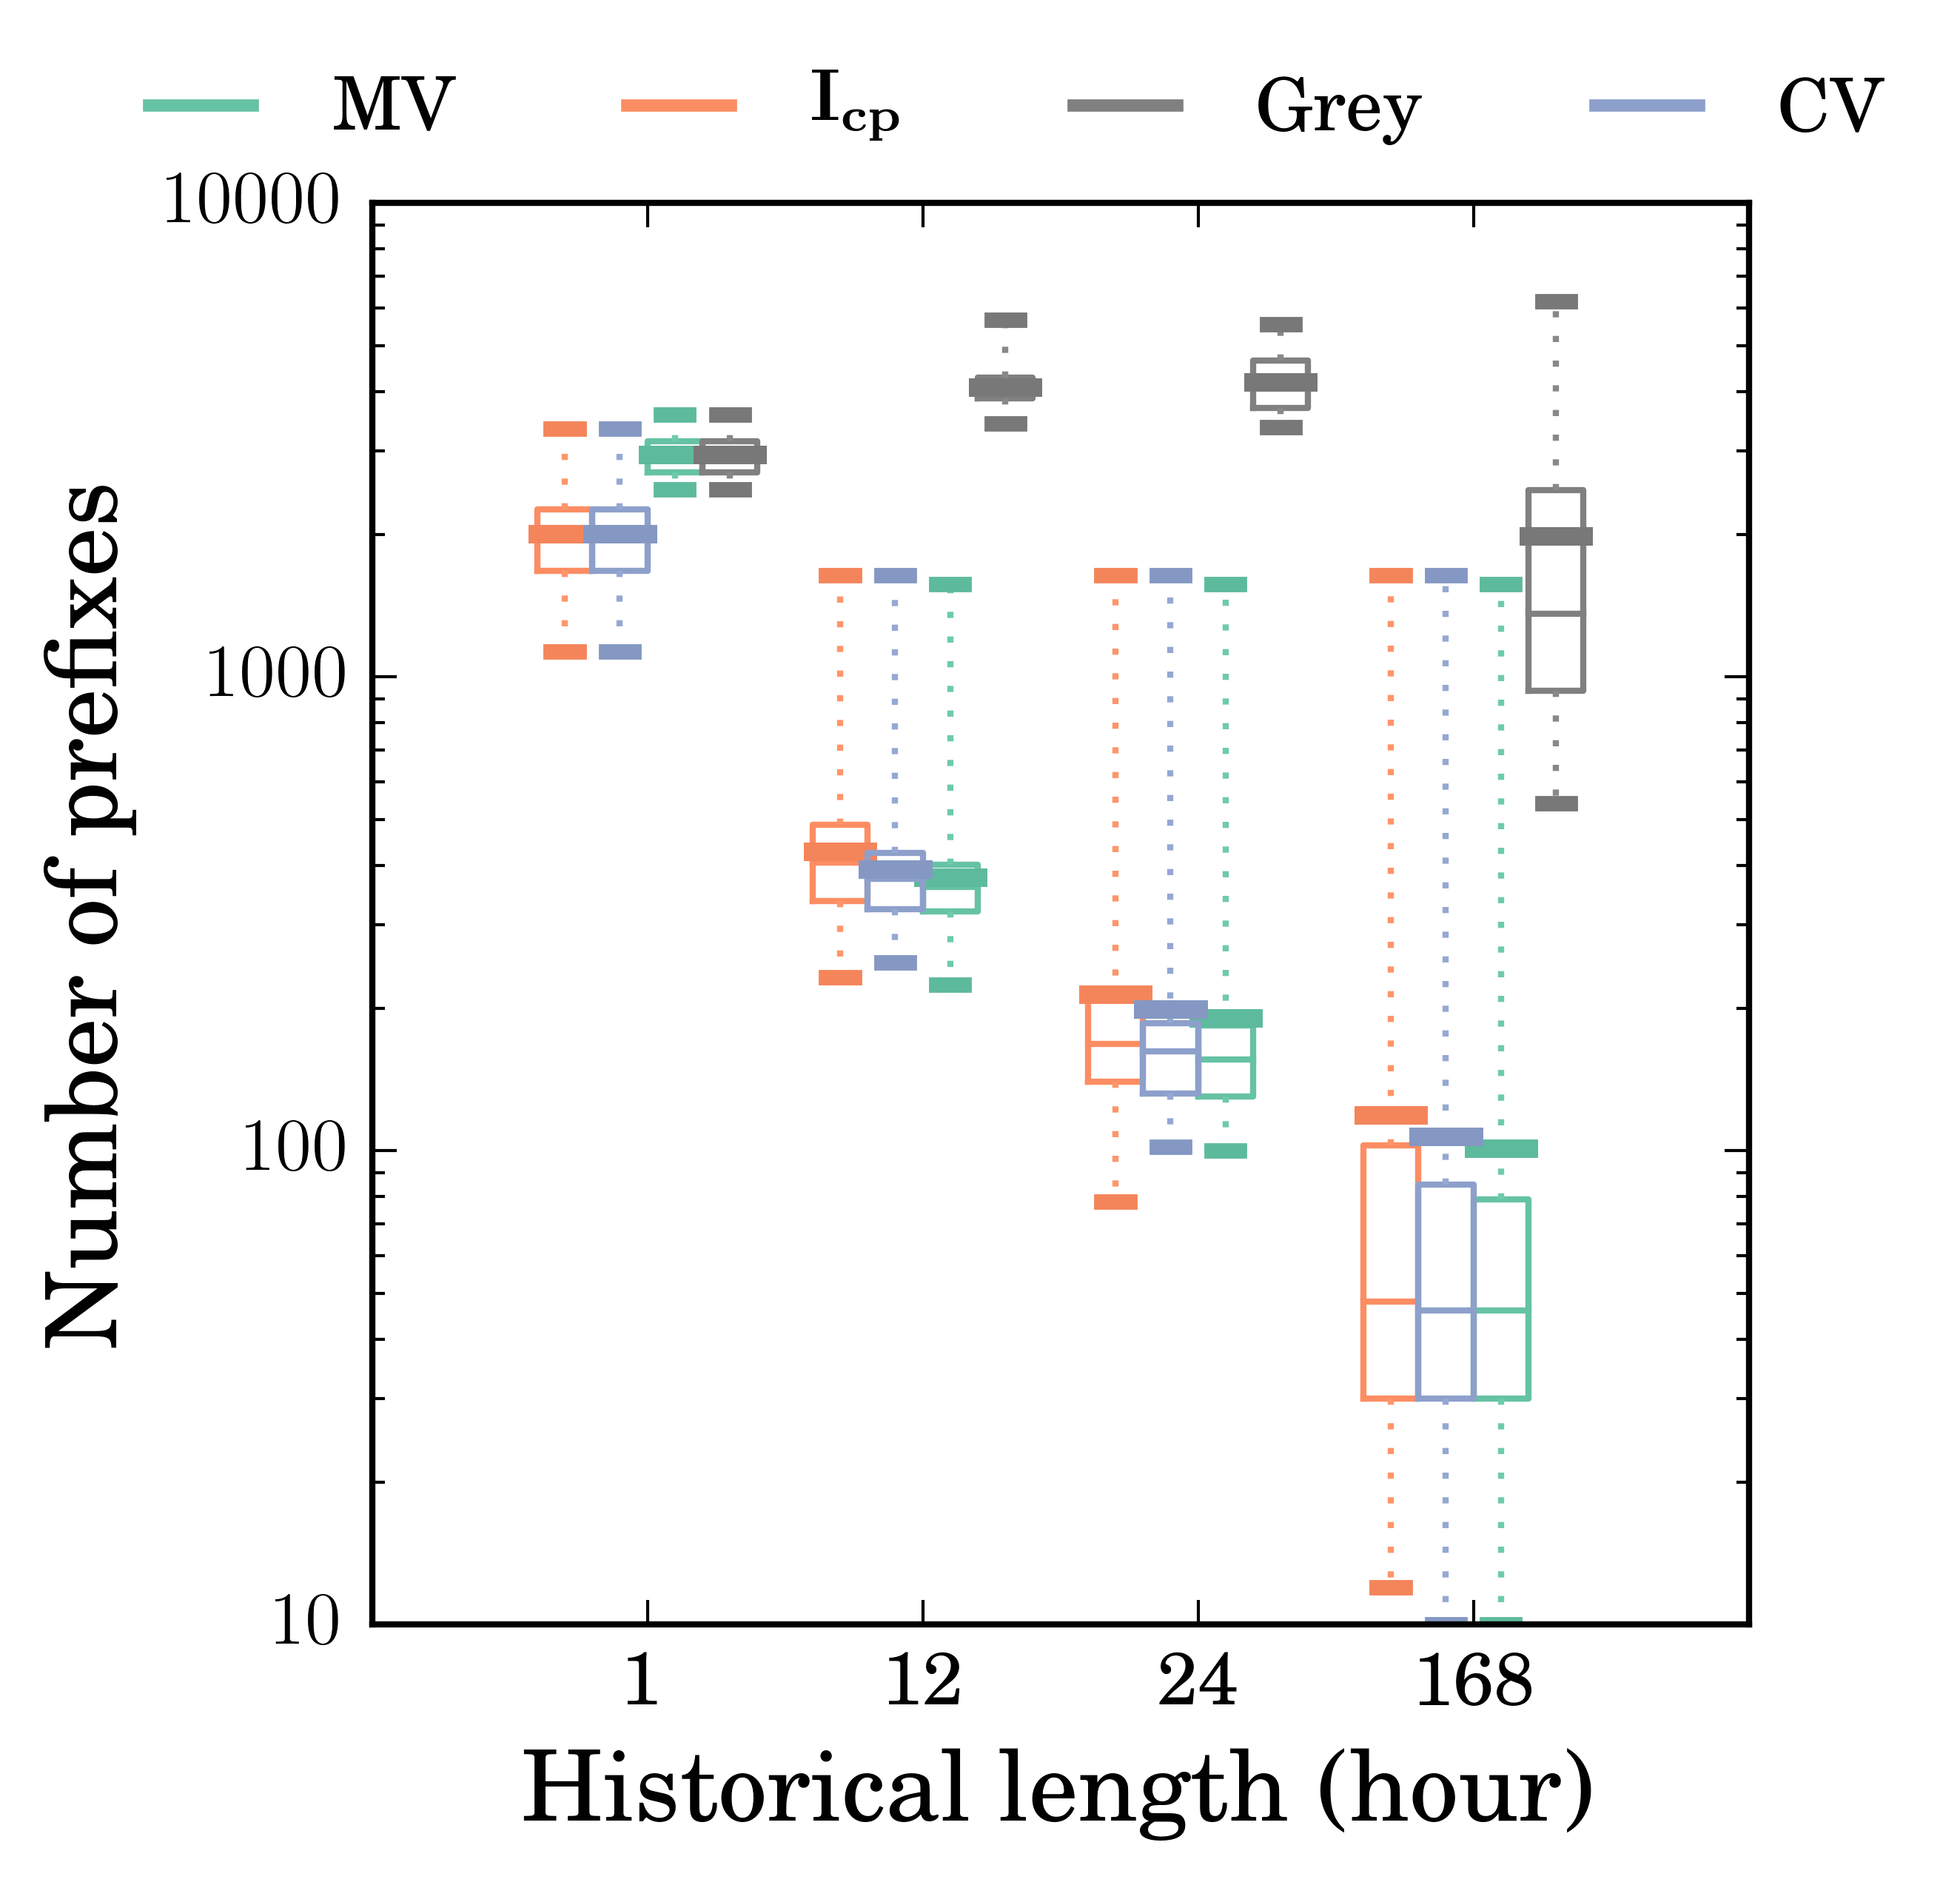
\includegraphics[width=\textwidth]{gfx/chap2/grey_churn_box_method_compare_fs_sd.png}
                \caption{SD}
                \label{fig:churn_sd}
        \end{subfigure}
        \begin{subfigure}[b]{0.48\textwidth}
                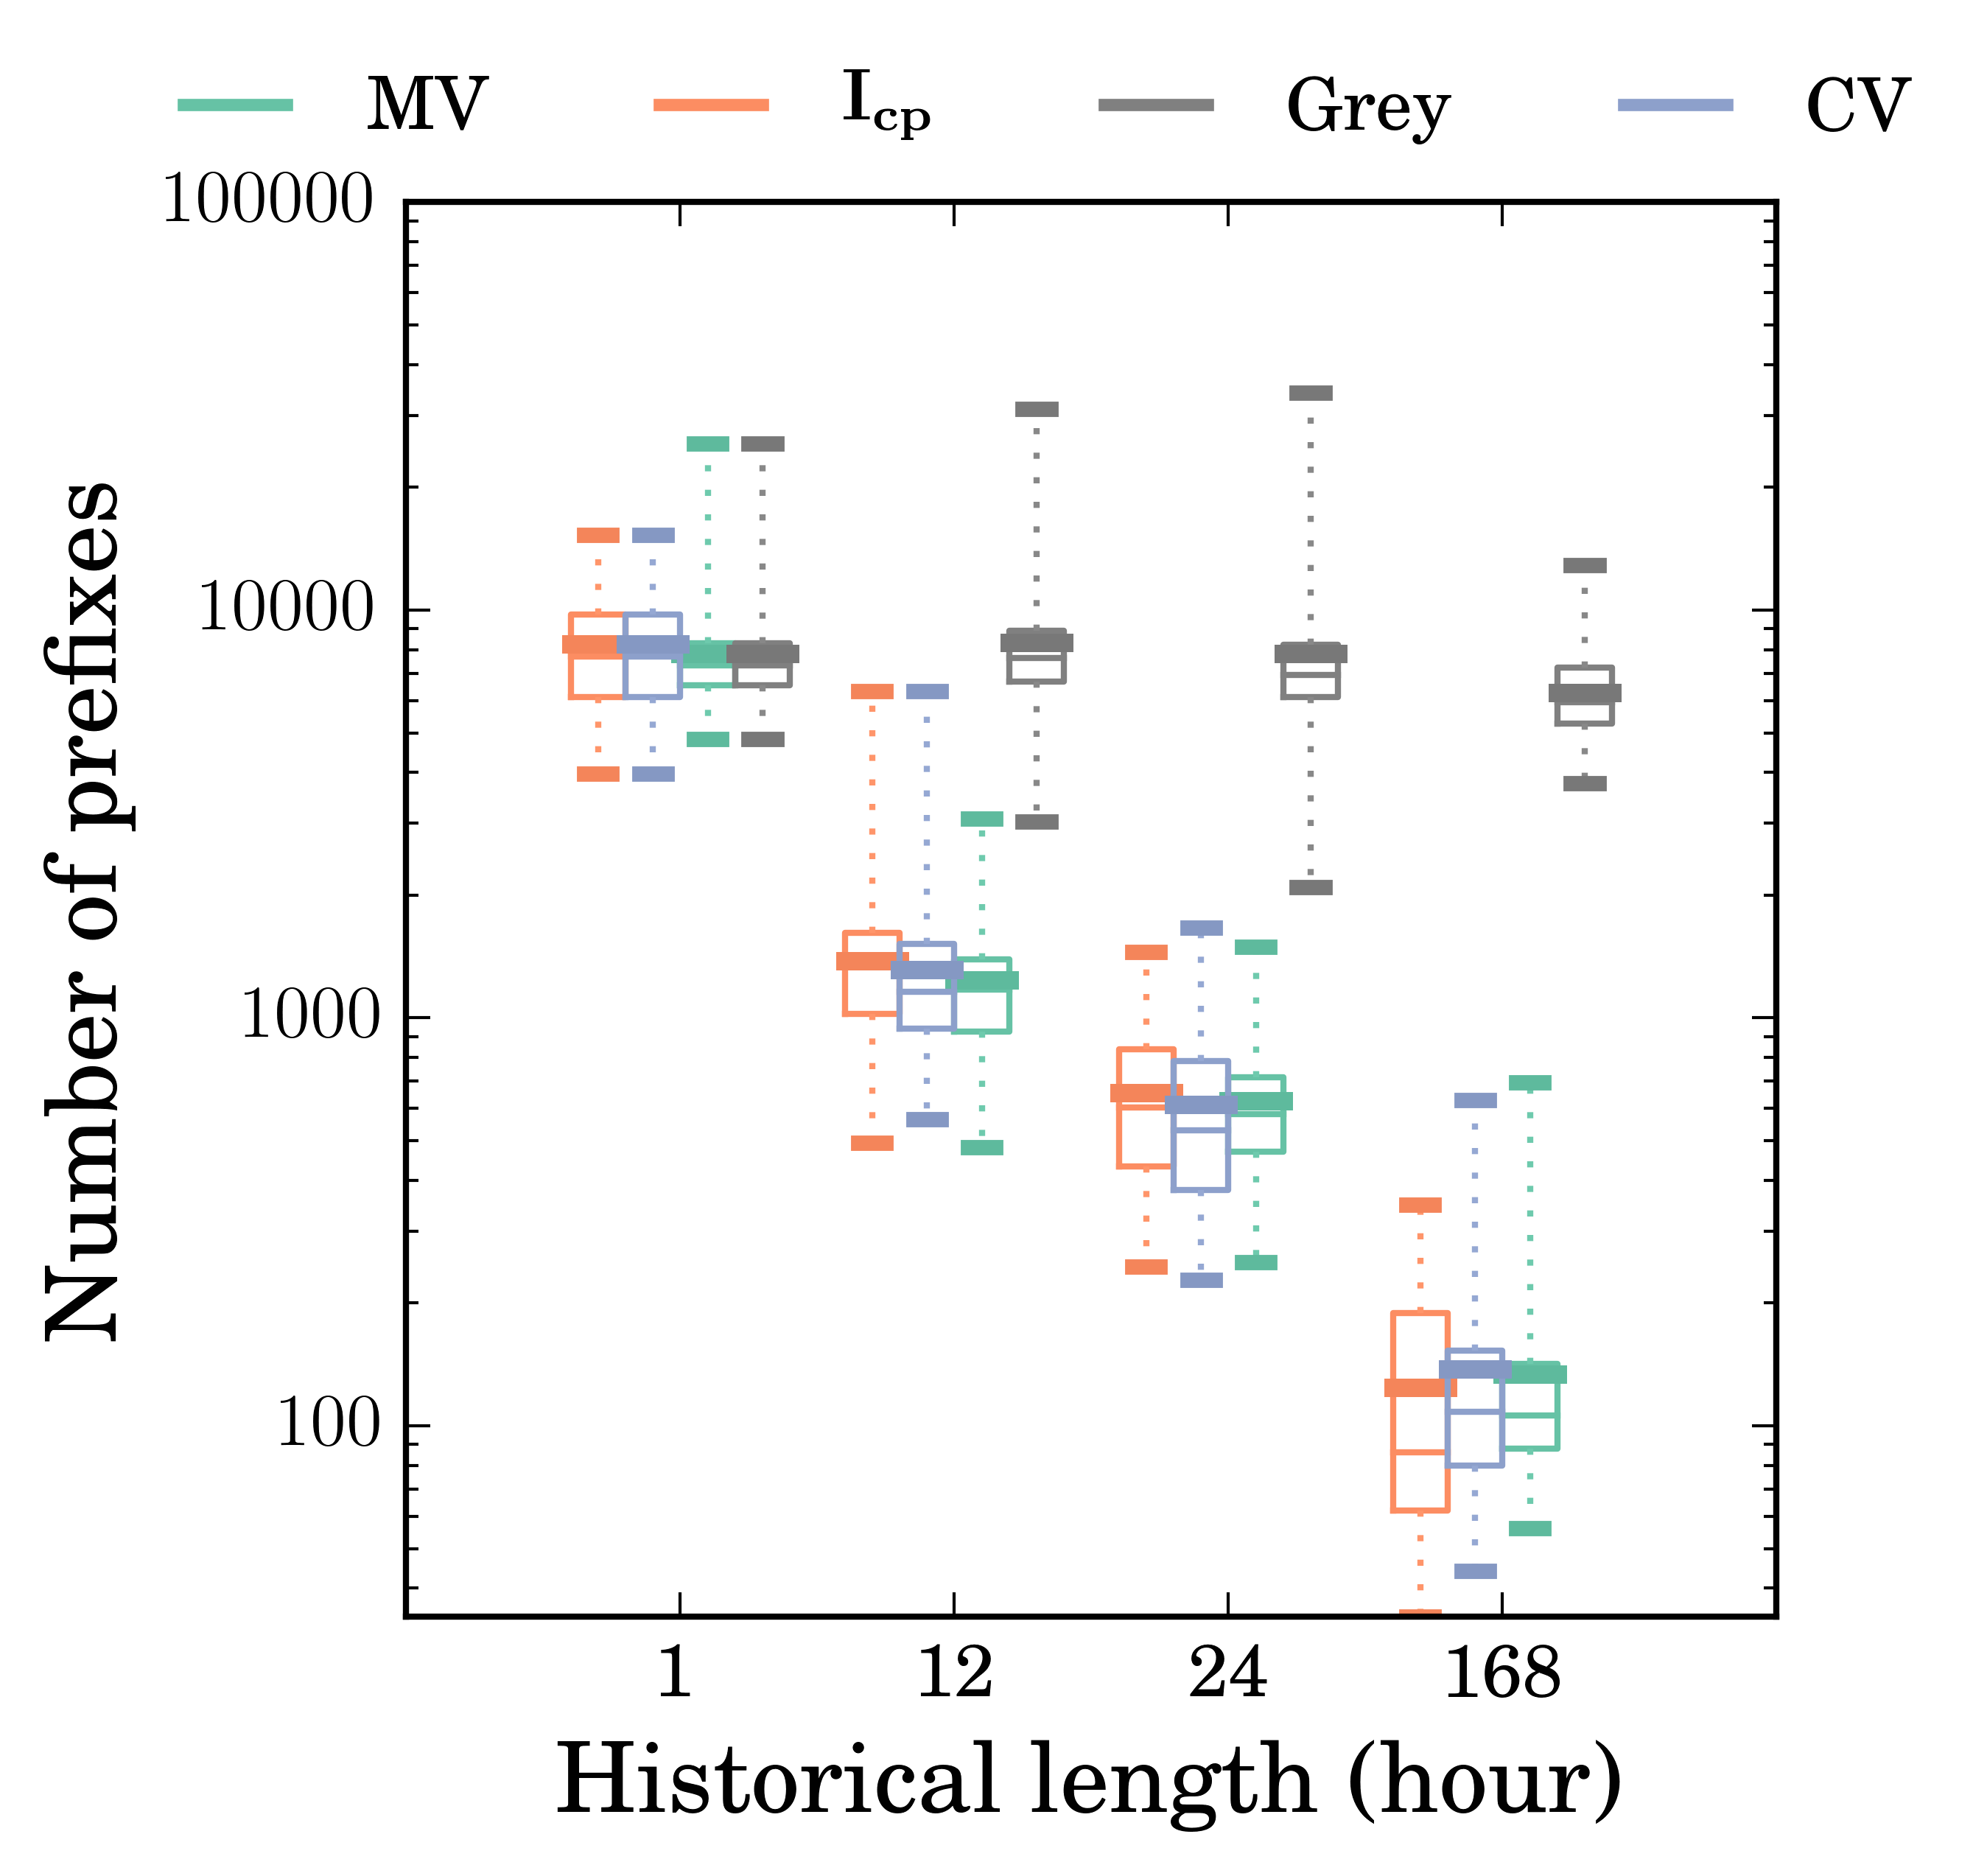
\includegraphics[width=\textwidth]{gfx/chap2/grey_churn_box_method_compare_fs_se.png}
                \caption{SE}
                \label{fig:churn_se}
        \end{subfigure}
        \begin{subfigure}[b]{0.48\textwidth}
                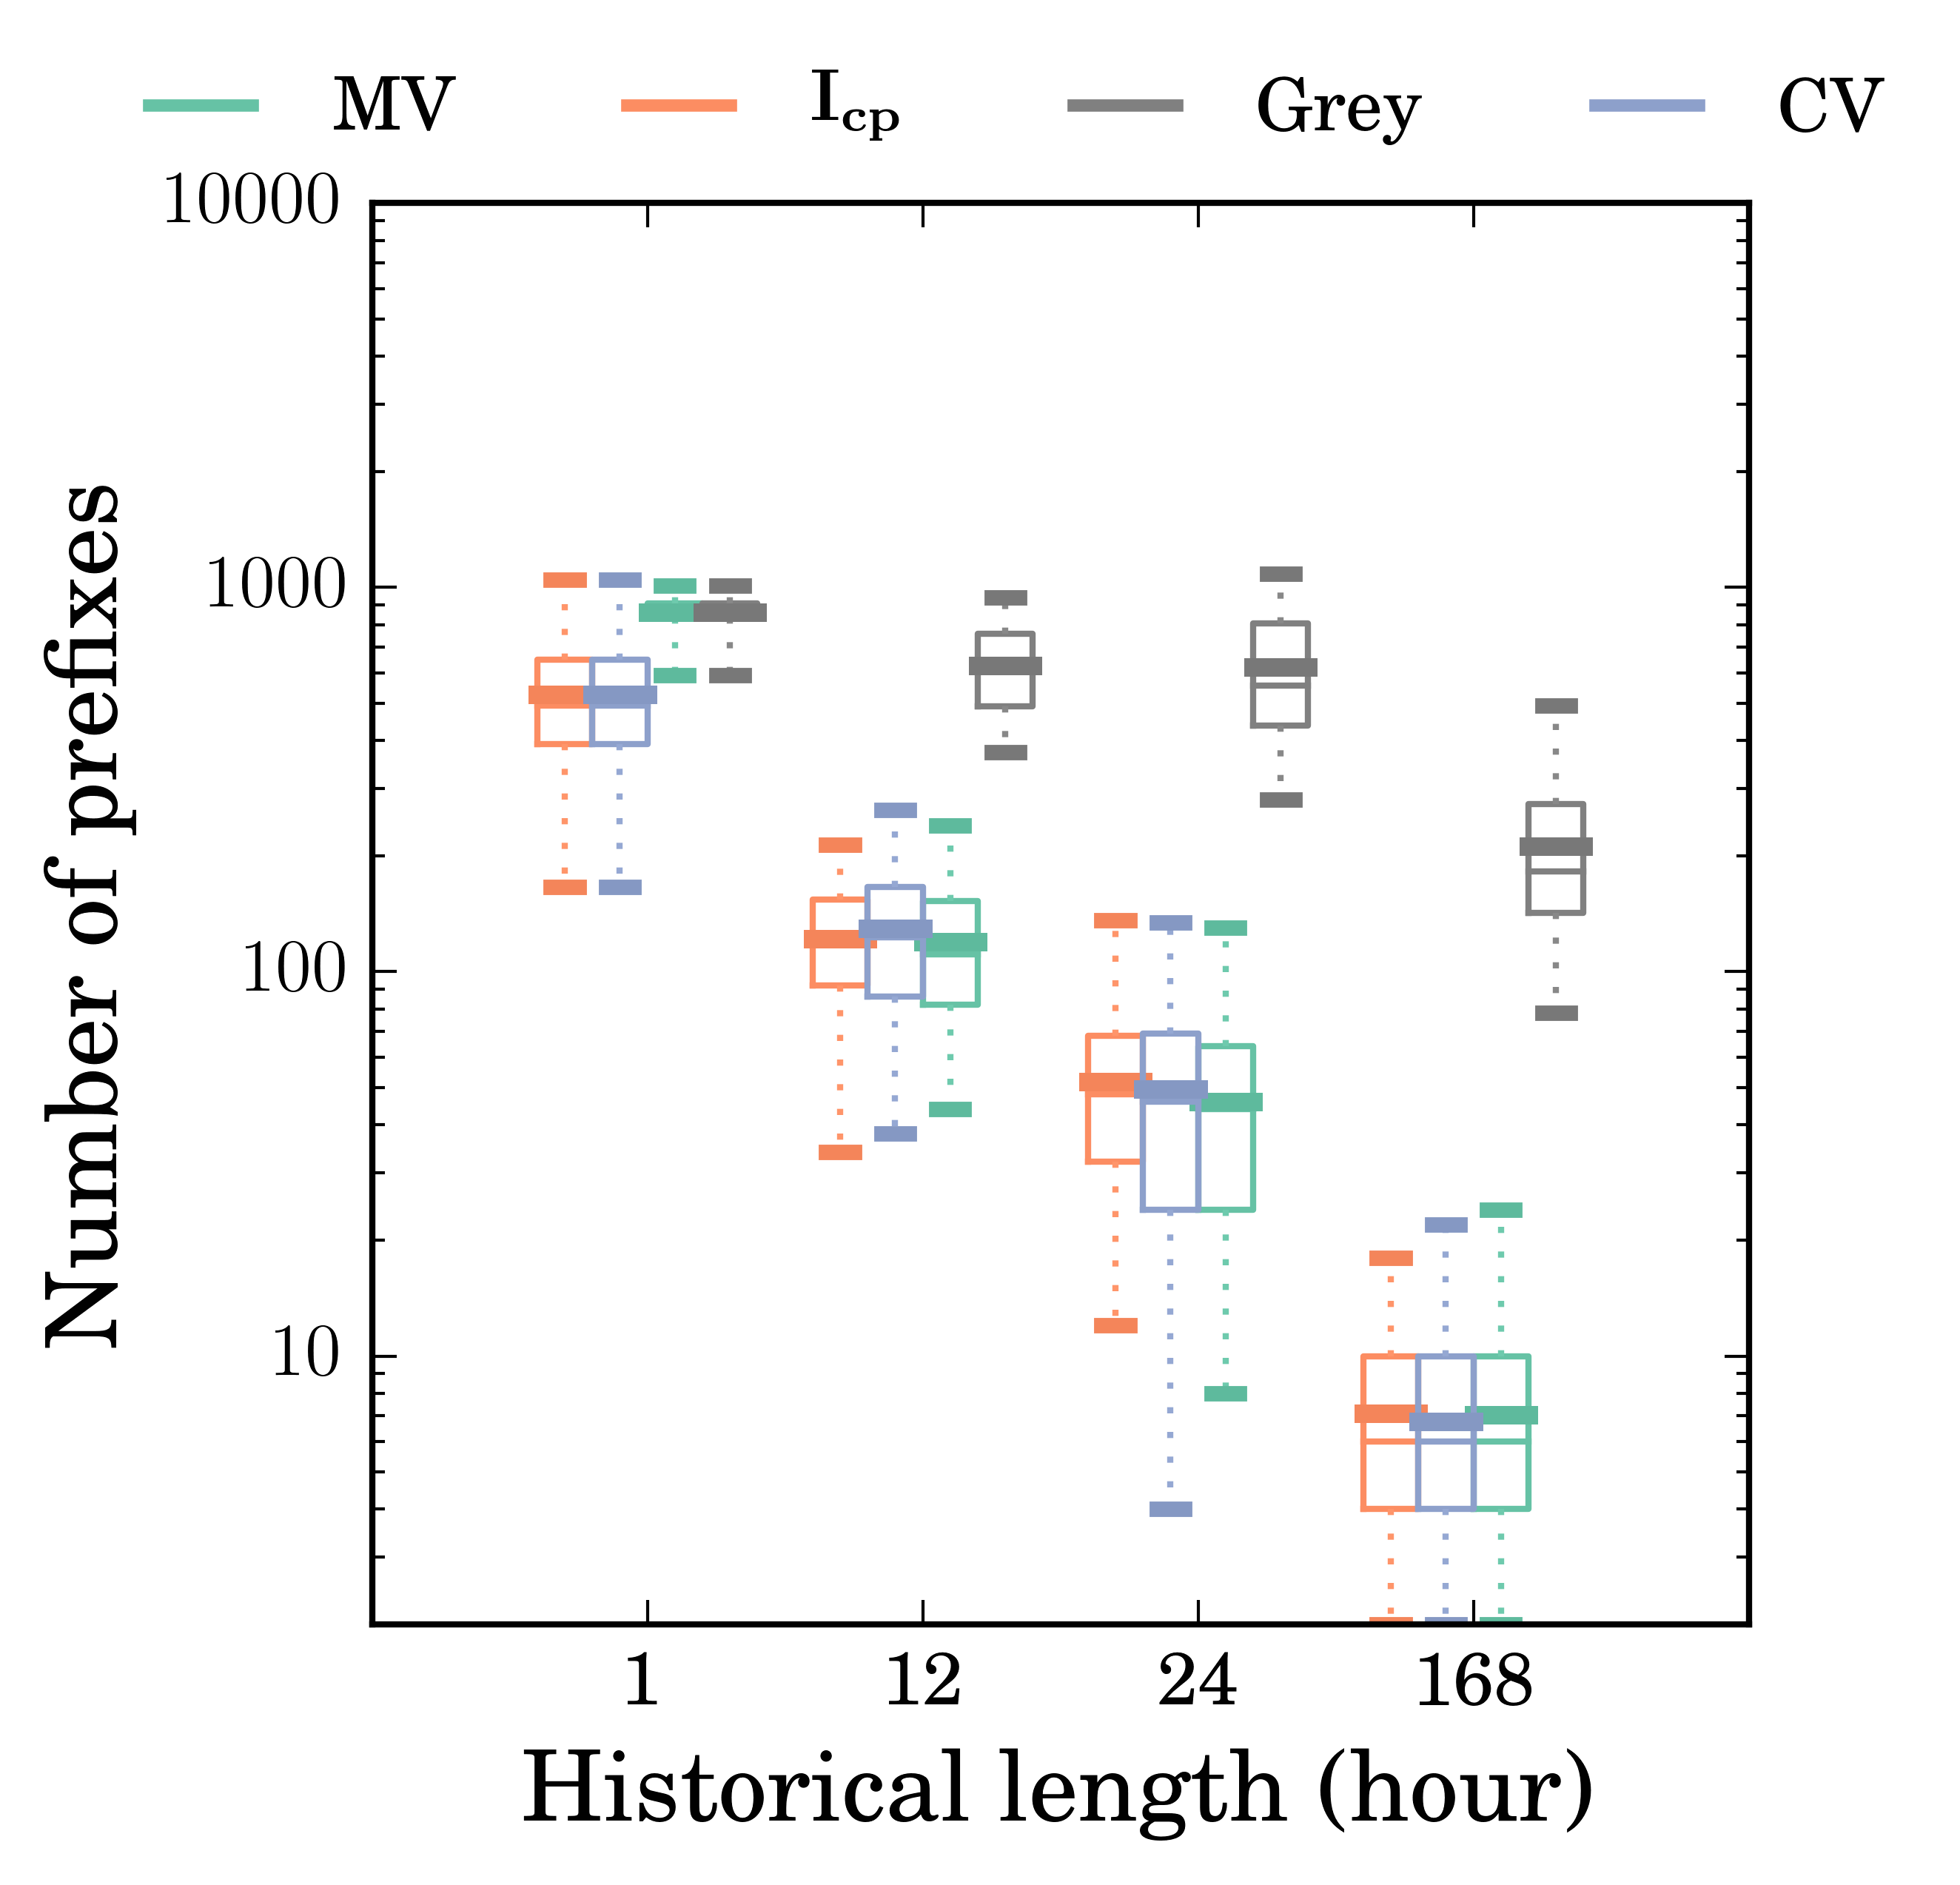
\includegraphics[width=\textwidth]{gfx/chap2/grey_churn_box_method_compare_fs_sf.png}
                \caption{SF}
                \label{fig:churn_sf}
        \end{subfigure}
\caption{Hour churn of the prefix set predictively selected using historical records of different lengths. The selection set size of each network is set to the maximum \textit{core} size over the week starting from June 1st, 2015, see in Table~\ref{tab:core_size}.}
\label{fig:churn}
\end{figure}

\begin{figure}\ContinuedFloat
	\centering 
        \begin{subfigure}[b]{0.48\textwidth}
                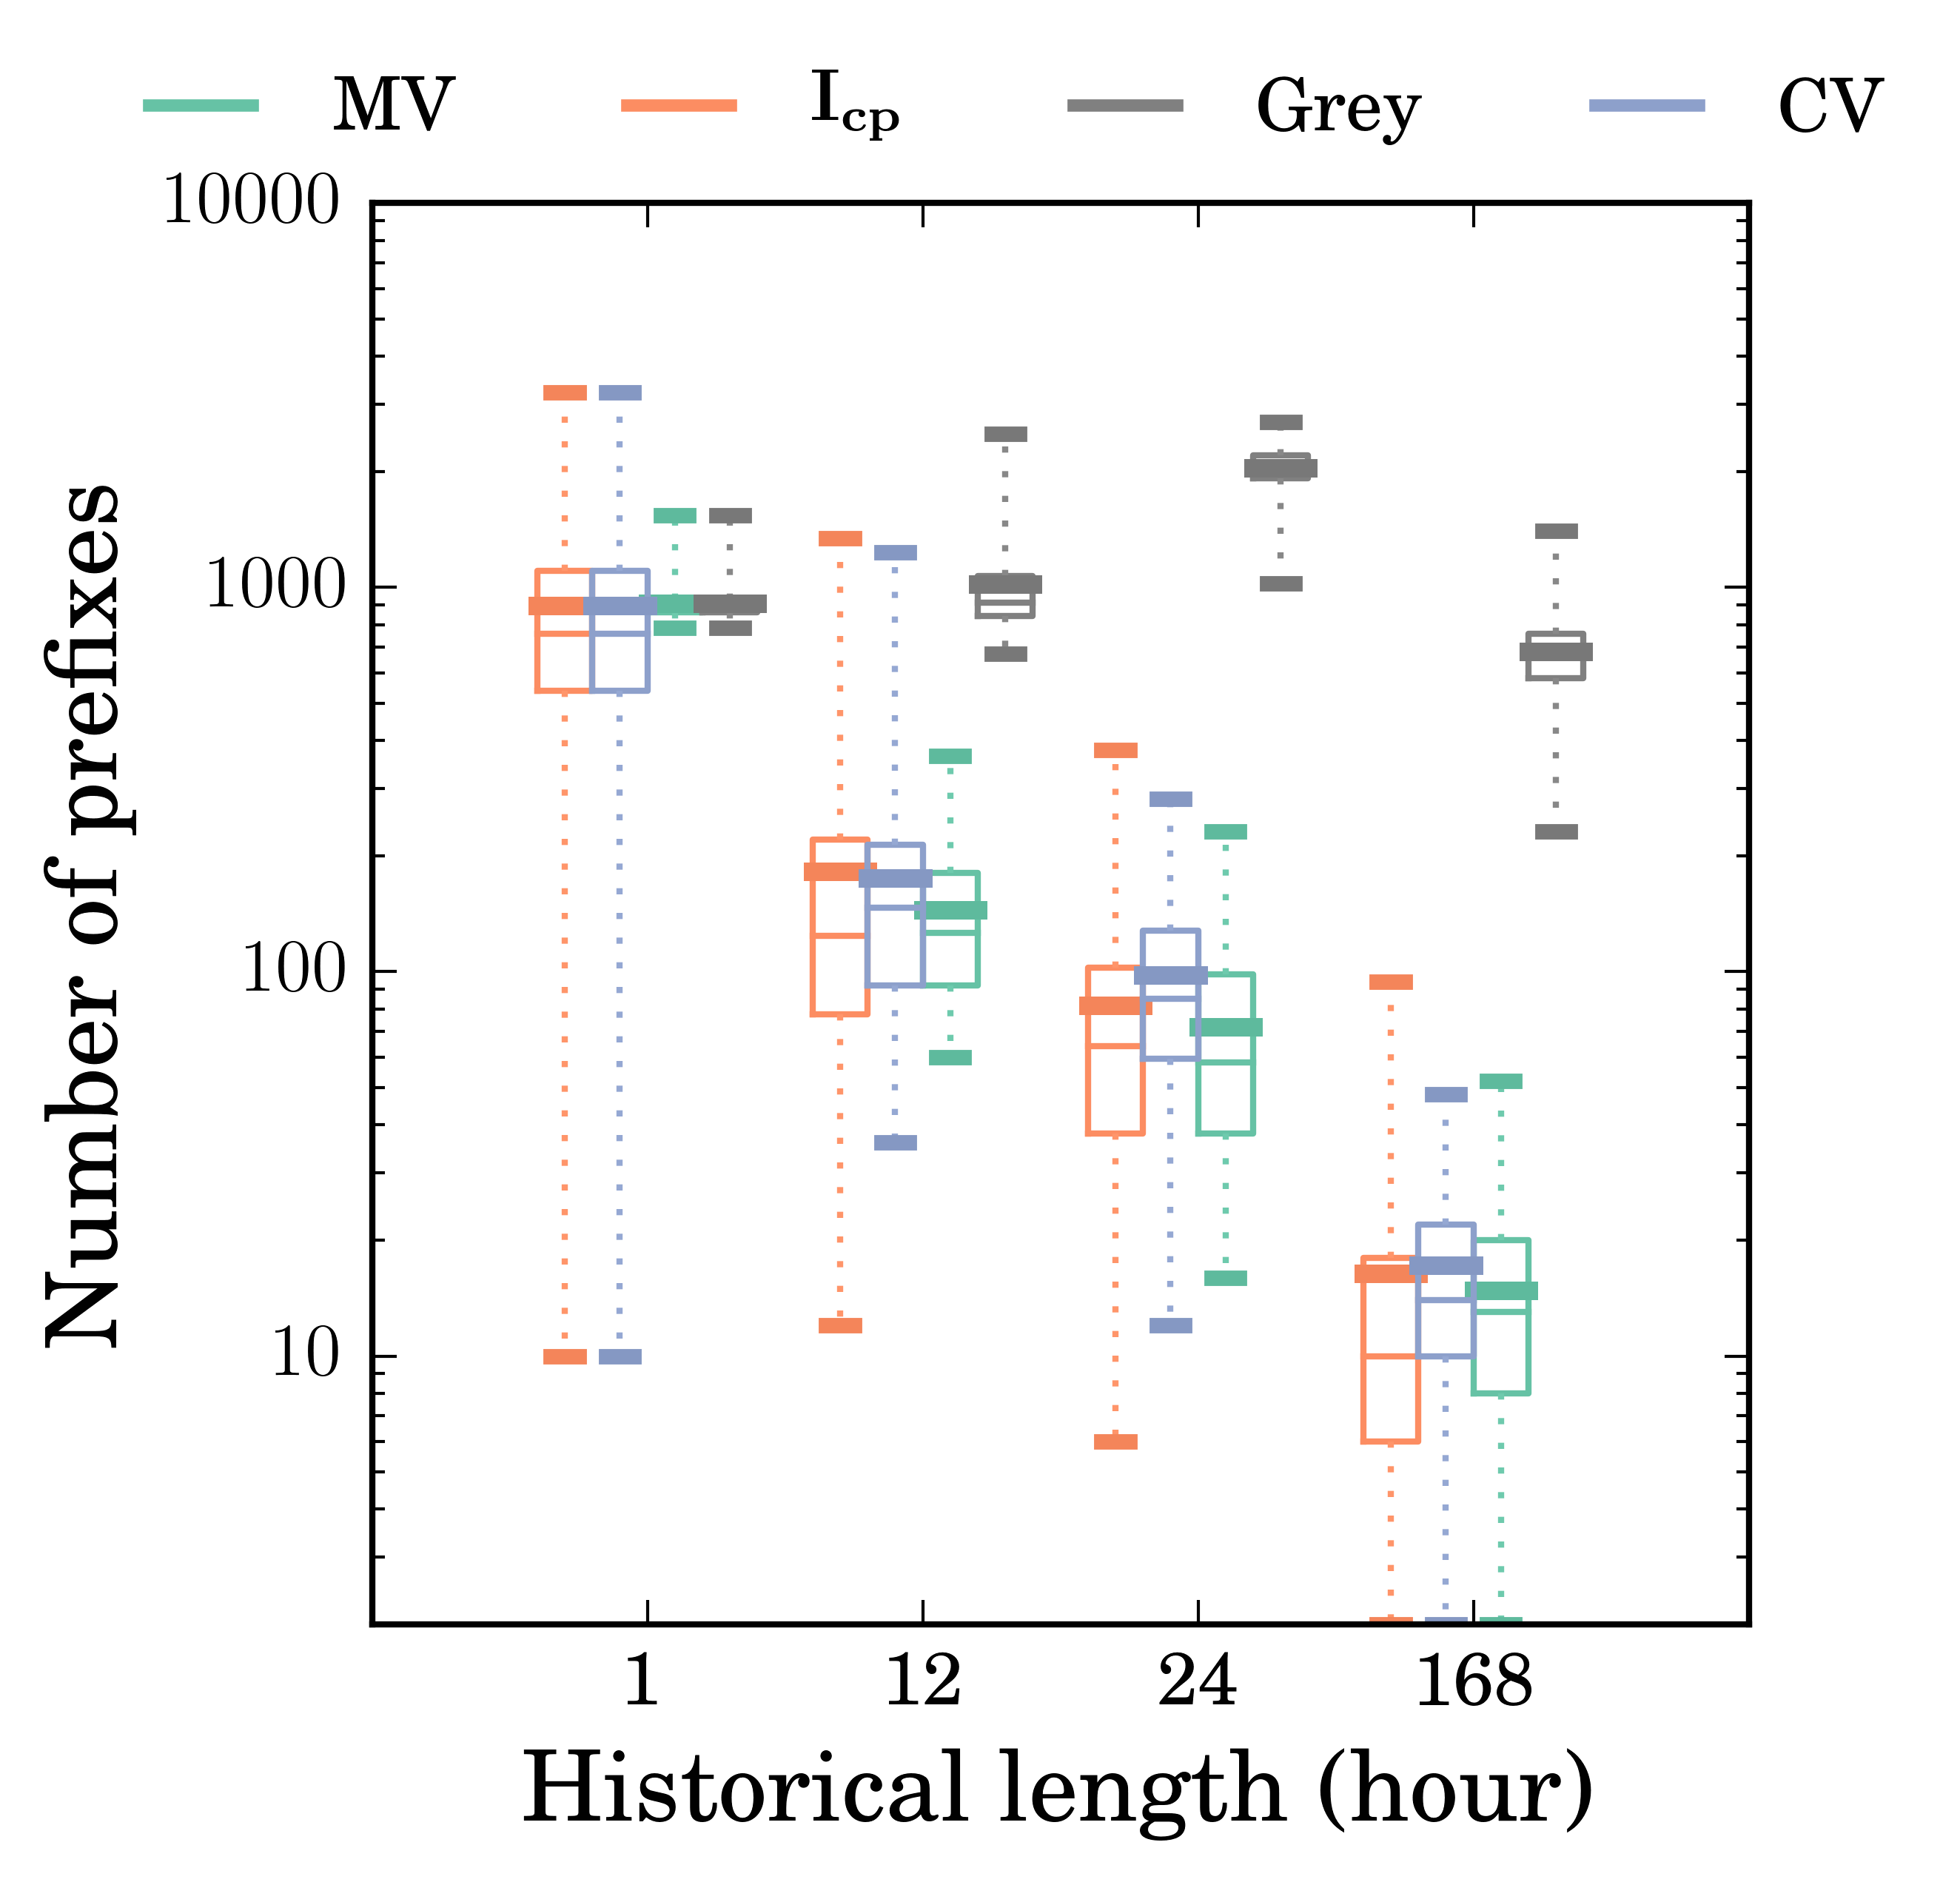
\includegraphics[width=\textwidth]{gfx/chap2/grey_churn_box_method_compare_fs_sg.png}
                \caption{SG}
                \label{fig:churn_sg}
        \end{subfigure}
        \begin{subfigure}[b]{0.48\textwidth}
                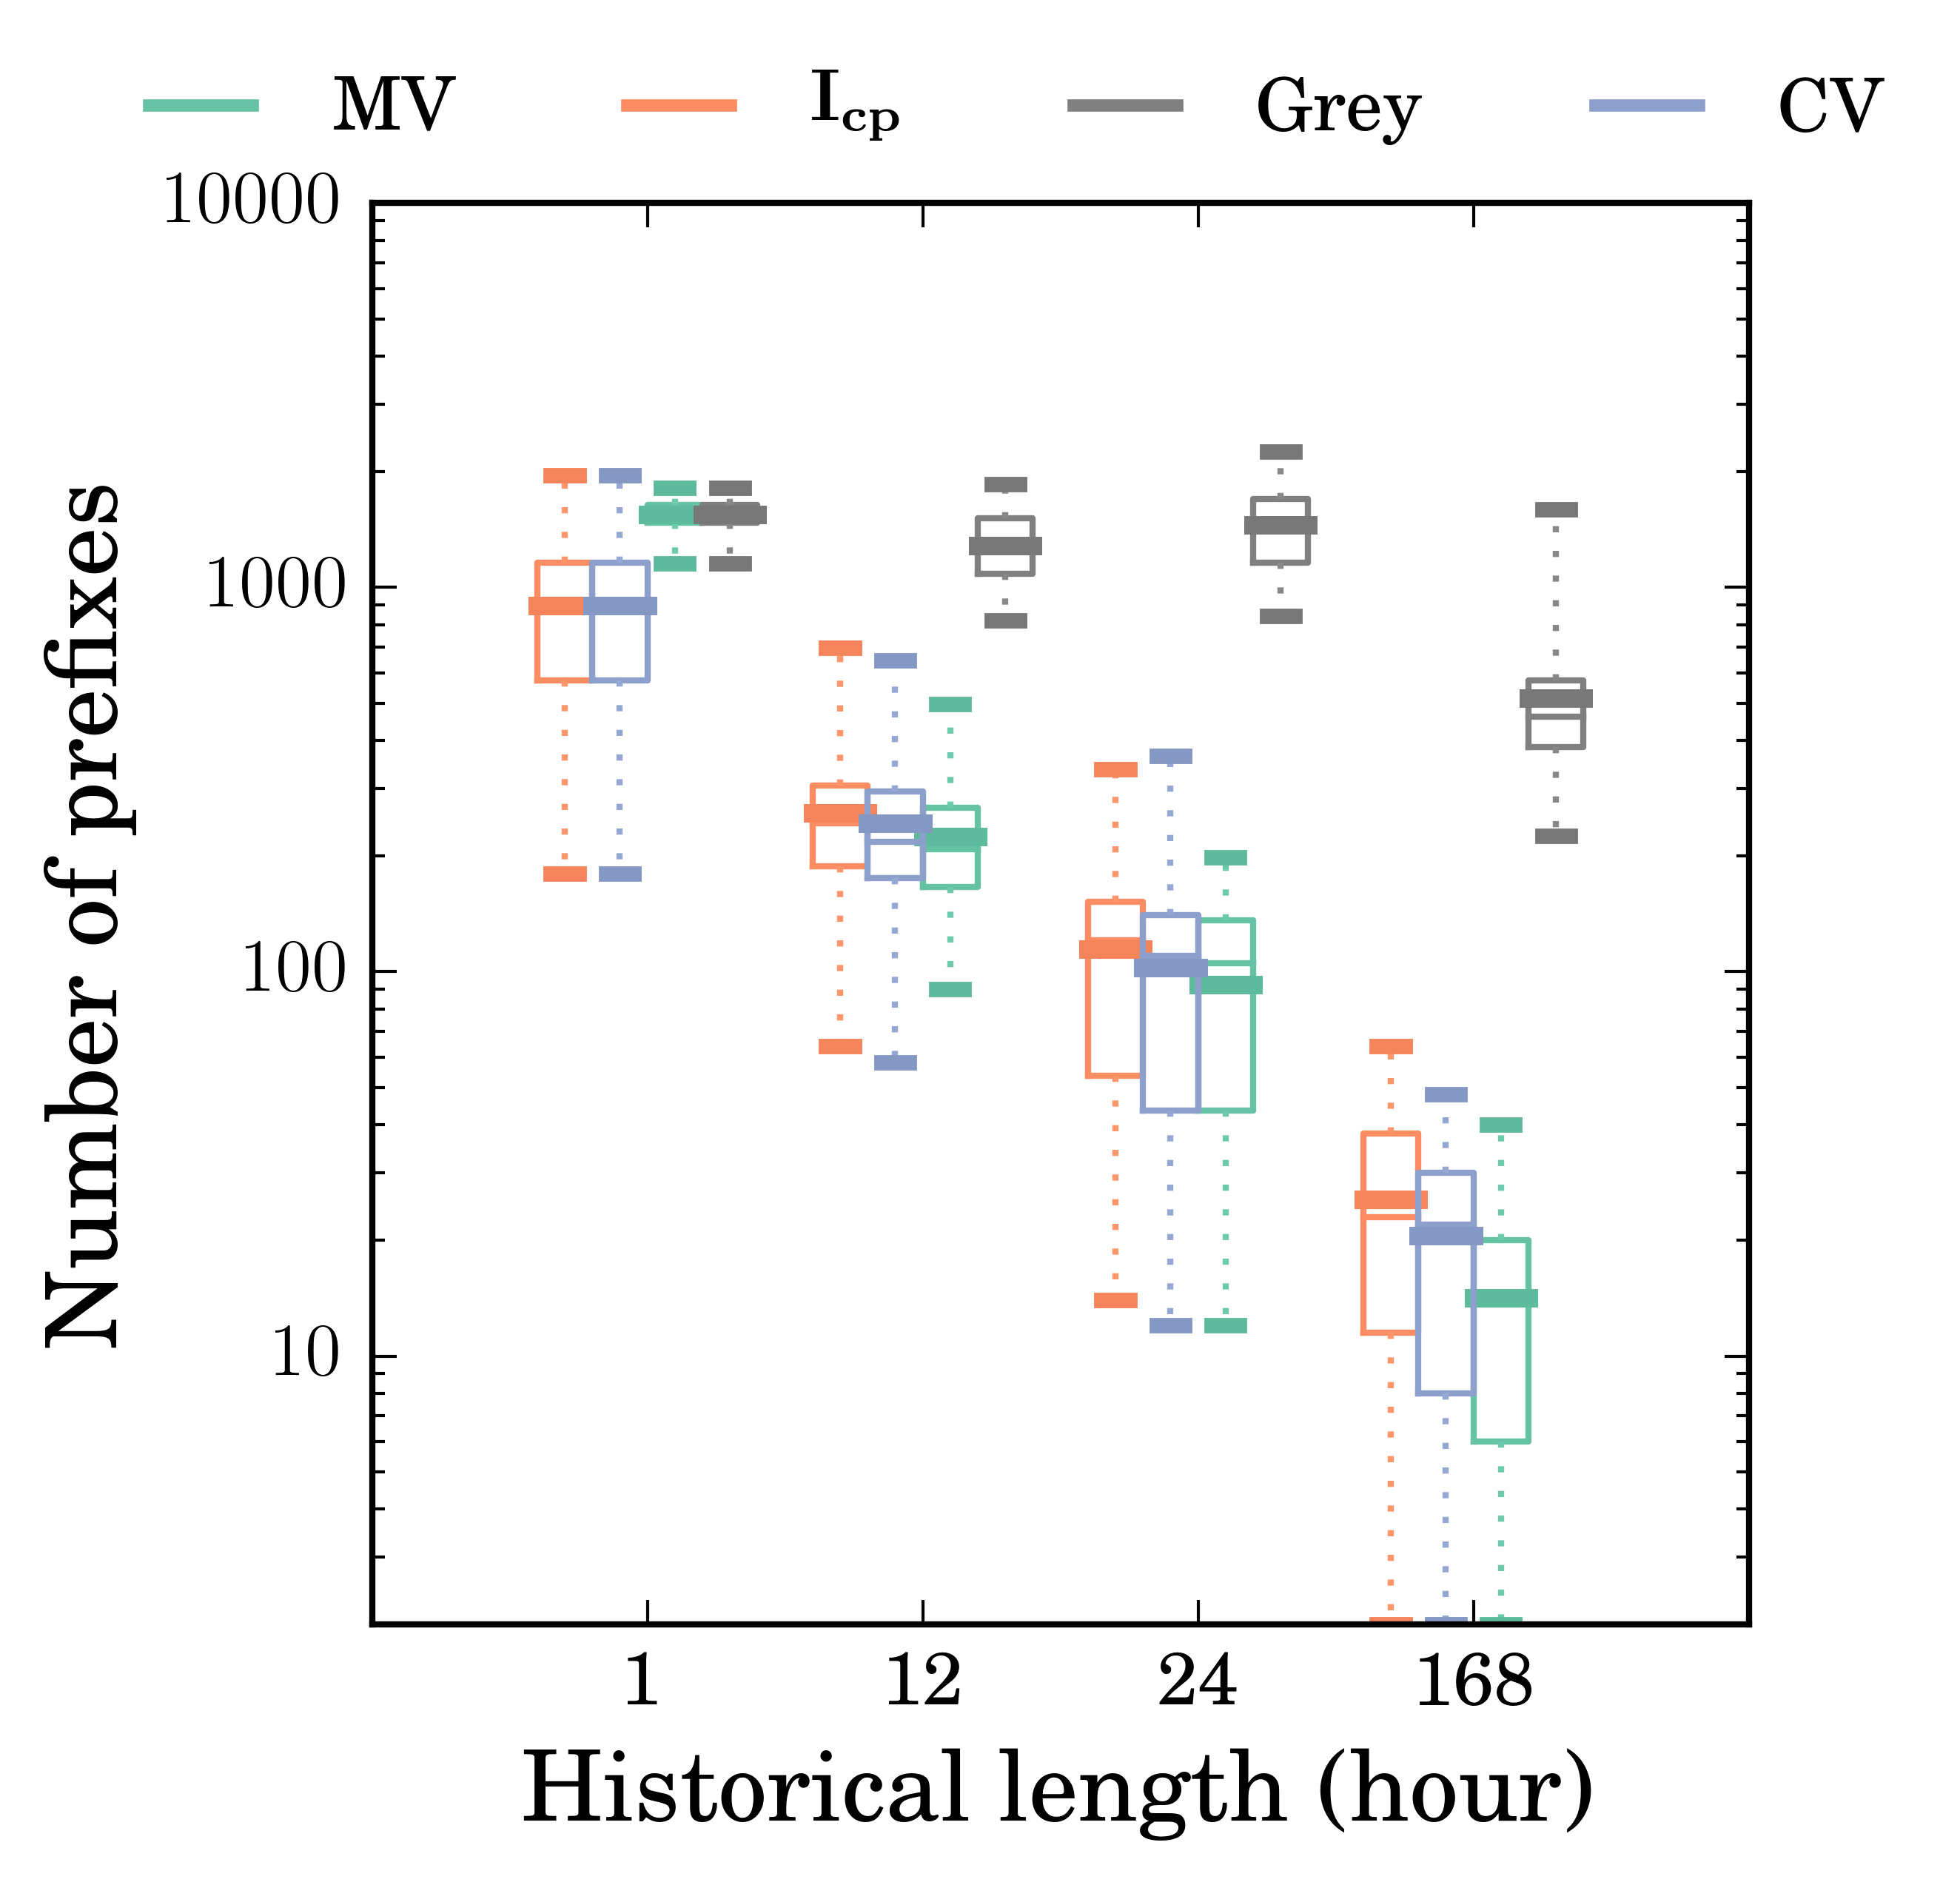
\includegraphics[width=\textwidth]{gfx/chap2/grey_churn_box_method_compare_fs_sh.png}
                \caption{SH}
                \label{fig:churn_sh}
        \end{subfigure}
        \begin{subfigure}[b]{0.48\textwidth}
                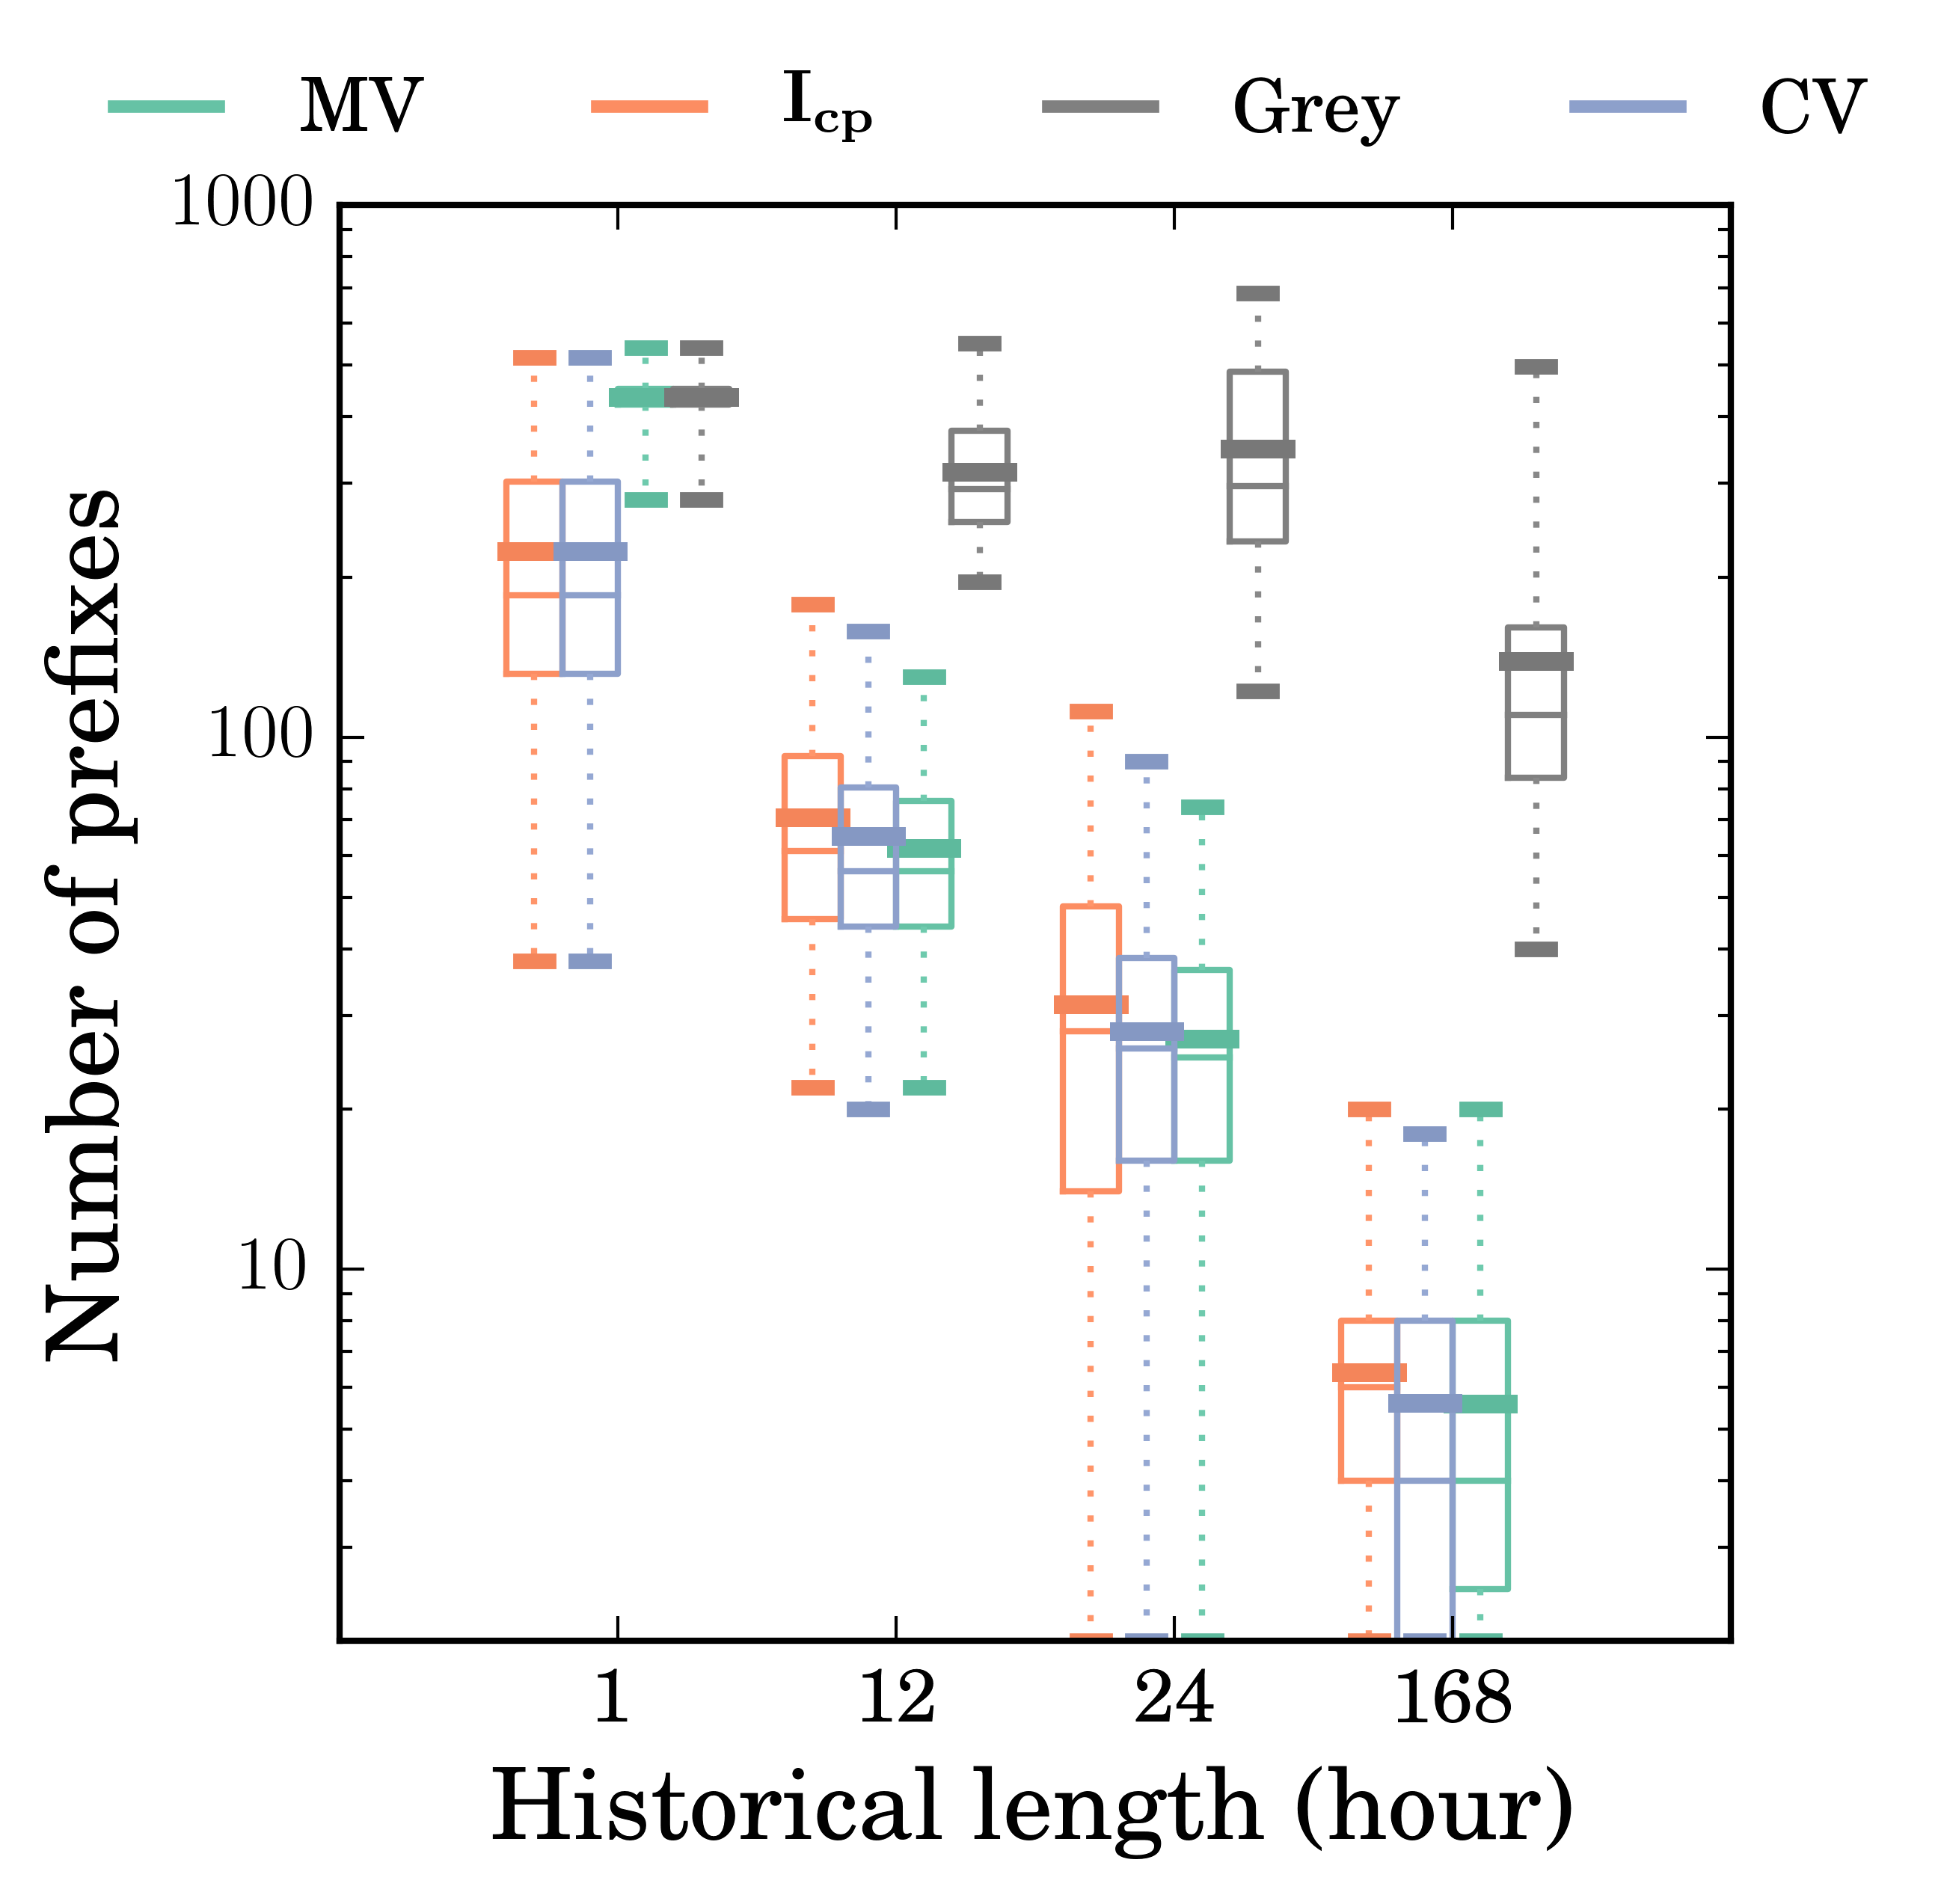
\includegraphics[width=\textwidth]{gfx/chap2/grey_churn_box_method_compare_fs_si.png}
                \caption{SI}
                \label{fig:churn_si}
        \end{subfigure}
\caption{(cont.) Hour churn of the prefix set predictively selected using historical records of different lengths.}
\label{fig:churn_cont}
\end{figure}

\marginpar{prefix churn}
Fig.~\ref{fig:churn} gives the results concerning the churn of the selection prefix set (in box-plot representation).
The churn is defined as the difference (i.e. number of new and deleted prefixes) between the new predicted set and the previous one. A high prefix churn is especially unwanted by the measurement sub-system, which aims at continuously monitoring and providing historical records of important destinations.  Sarrar et al.\ \cite{Sarrar2012} also argued that small prefix churn is very important in network architecture with decoupled forwarding and control planes, such as SDN (Software Defined Networking), as it leads to lower communication overhead.

\marginpar{discussion on historical length}
As expected, a clear drop of the churn value can be seen when the historical length increases --- as opposed to what happens with the grey model. 
In that sense, using long historical records can be a wise choice in practice.
Furthermore, for networks with relatively few bursty traffic, e.g. SA, the mean volume coverage with last 168 hour records is extremely close to that with last 24 hour records, shown  by Fig.~\ref{fig:cvg_sa}.
Finally, for networks with highly bursty traffic, SC, using long records has the potential to obviously improve worst-case volume coverage. 

In the purpose of lowering churn, Sarrar et al.\ \cite{Sarrar2012} proposed selecting top prefixes over time bins of different lengths (ranging from 1 second to 10 minute in their FIB-caching environment). In our context, we found that the difference in mean volume coverage using record lengths larger than 1 hour is marginal, thus little gain can be expected from this method.  

%\begin{table*}[!htb]
%\centering
%\begin{tabular}{cc|cc|cc}\toprule
%\textbf{Network} & \textbf{$L$}  & \textbf{Mean Cvg.} & \textbf{Min Cvg.} & \textbf{Mean Churn} & %\textbf{Max Churn}\\
%\midrule
%SA & 24   & 93.73 & 85.32 & 32.23  & 148\\
%SB & 24   & 88.02 & 79.82 & 873.11 & 4026\\
%SC & 168  & 88.73 & 61.11 & 2.84   & 10\\
%SD & 168  & 83.22 & 69.23 & 107.06 & 1642\\
%SE & 24   & 90.51 & 78.85 & 613.72 & 1664 \\
%SF & 24   & 81.33 & 51.94 & 49.52  & 134\\
%SG & 168  & 86.44 & 52.60 & 17.24  & 48\\
%SH & 24   & 92.04 & 81.21 & 102.60 & 364\\
%SI & 24   & 87.71 & 66.75 & 28.01  & 90\\
%\bottomrule
%\end{tabular}
%\caption{Hourly volume coverage (in percentage) and churn, using \text{core} volume metric $CV$ with record length $L$ yielding the highest mean coverage.}
%\label{tab:cvg_churn}
%\end{table*}

%Among all the networks, we achieved the best mean volume coverage under $CV$ metric ($>92\%$) on SA and SH, as it can seen in Table~\ref{tab:cvg_churn}. 
%This corresponds to the fact that these two networks suffers the lest from bursty traffic.

\subsubsection{Relation between volume coverage and traffic burstiness}

\begin{figure}[!tb]
\centering
		\centering
        \begin{subfigure}[b]{0.42\textwidth}
        \centering
                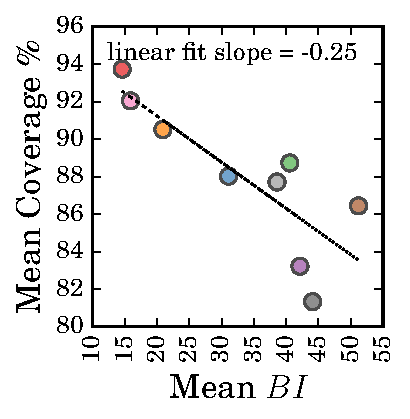
\includegraphics[width=\textwidth]{gfx/chap2/bi_cvg_mean.pdf}
                \caption{Average level}
                \label{fig:bi_cvg_mean}
        \end{subfigure}
        \hfill
        \begin{subfigure}[b]{0.53\textwidth}
                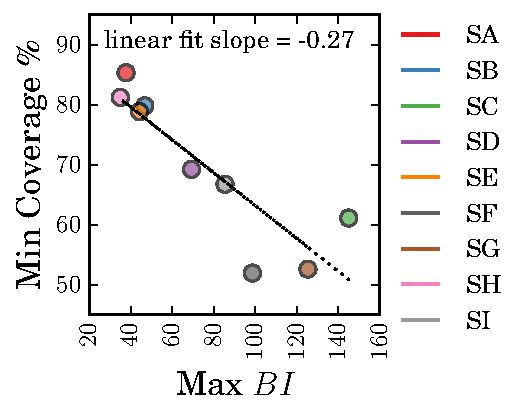
\includegraphics[width=\textwidth]{gfx/chap2/bi_cvg_worst.pdf}
                \caption{Worst case}
                \label{fig:bi_cvg_worst}
        \end{subfigure}
\caption{The relationship between burstiness index $BI$ and traffic volume coverage of selected prefix using $CV$ metric.}
\label{fig:bi_cvg}
\end{figure}

Finally, in Fig.~\ref{fig:bi_cvg} the mean/minimum coverage achieved with $CV$ metric is showed as a function of the $BI$ index. We can see that the mean (resp. minimum) coverage is inversely proportional to the mean (resp. maximum) $BI$ index. As expected, this graphic highlight the difficulty to cover an important fraction of traffic volume for networks with more bursty traffic. However, the quasi-linear curve obtained shows that $BI$ is a very meaningful metric to identify sites with bursty trafic. For large $BI$ values, it can be worthy of choosing a larger prefix set size (which was previously fixed to the weekly maximum core size), if possible. 

\section{Transit provider performance evaluation}
\label{sec:rtt}

\begin{figure}
\centering
		\centering
        \begin{subfigure}[b]{0.48\textwidth}
                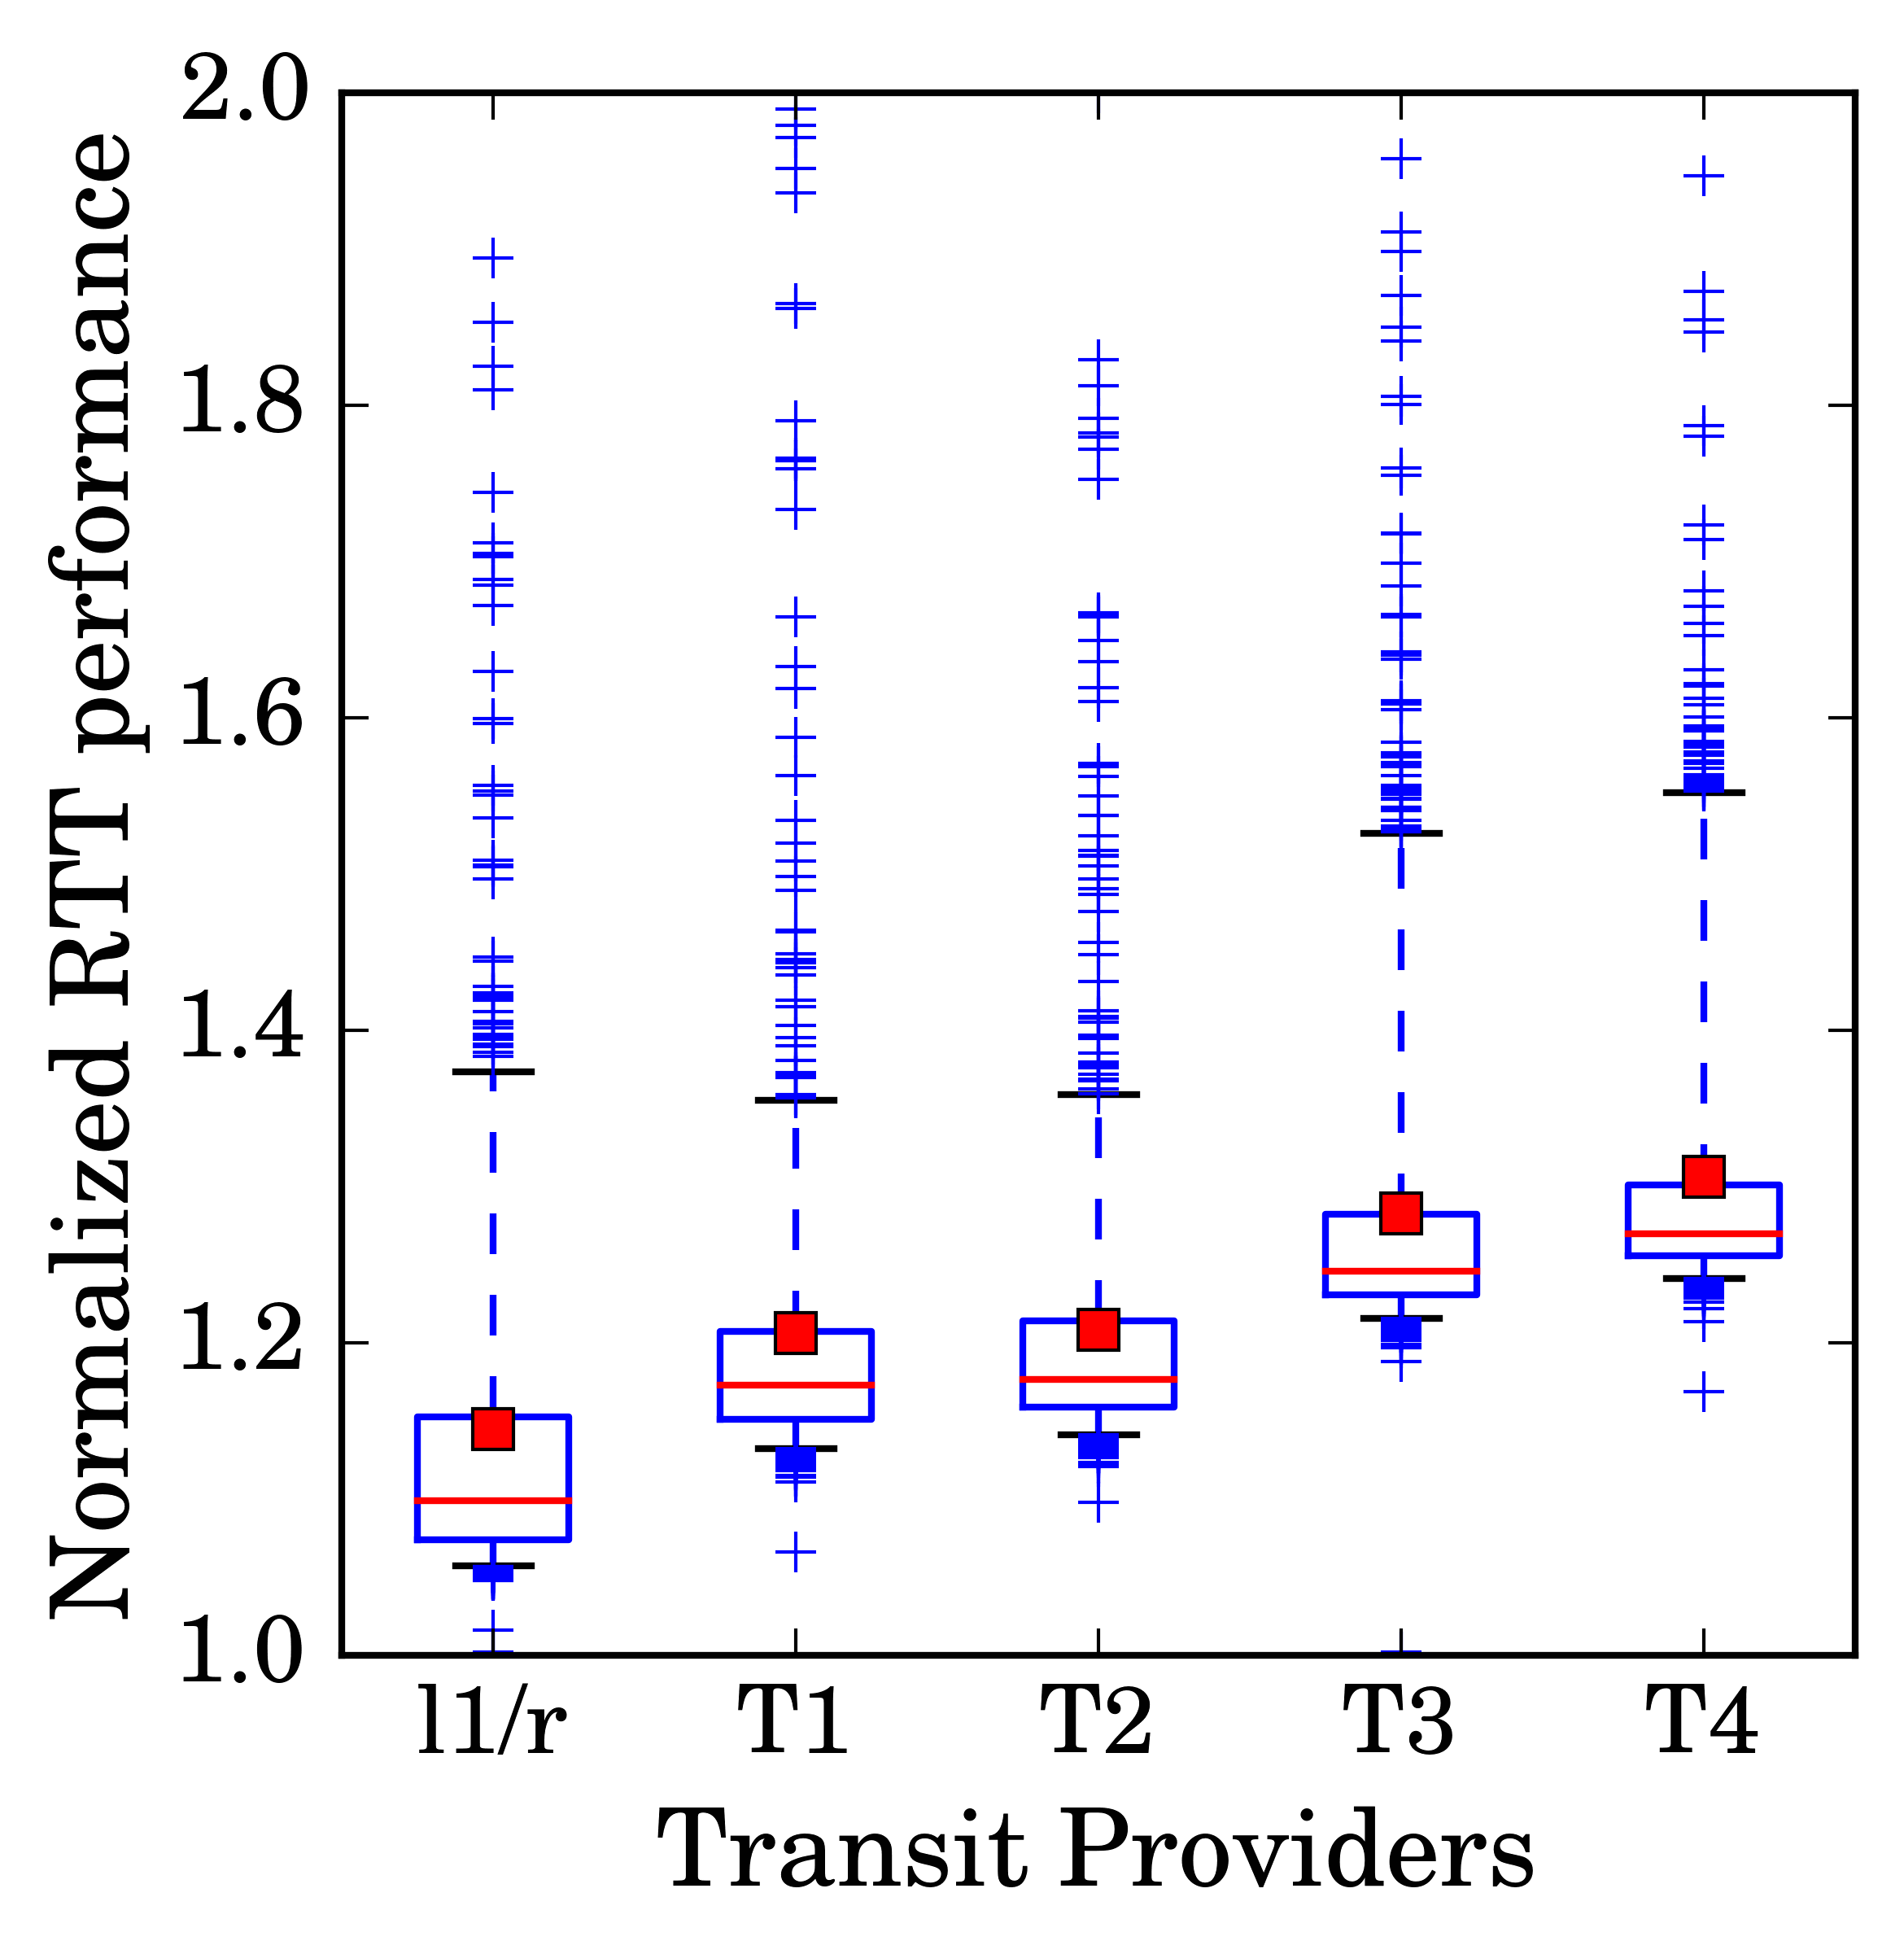
\includegraphics[width=\textwidth]{gfx/chap2/np_box_sa.png}
                \caption{SA, 866 prefixes, $85.69\%$ traffic}
                \label{fig:np_sa}
        \end{subfigure}
        \begin{subfigure}[b]{0.48\textwidth}
                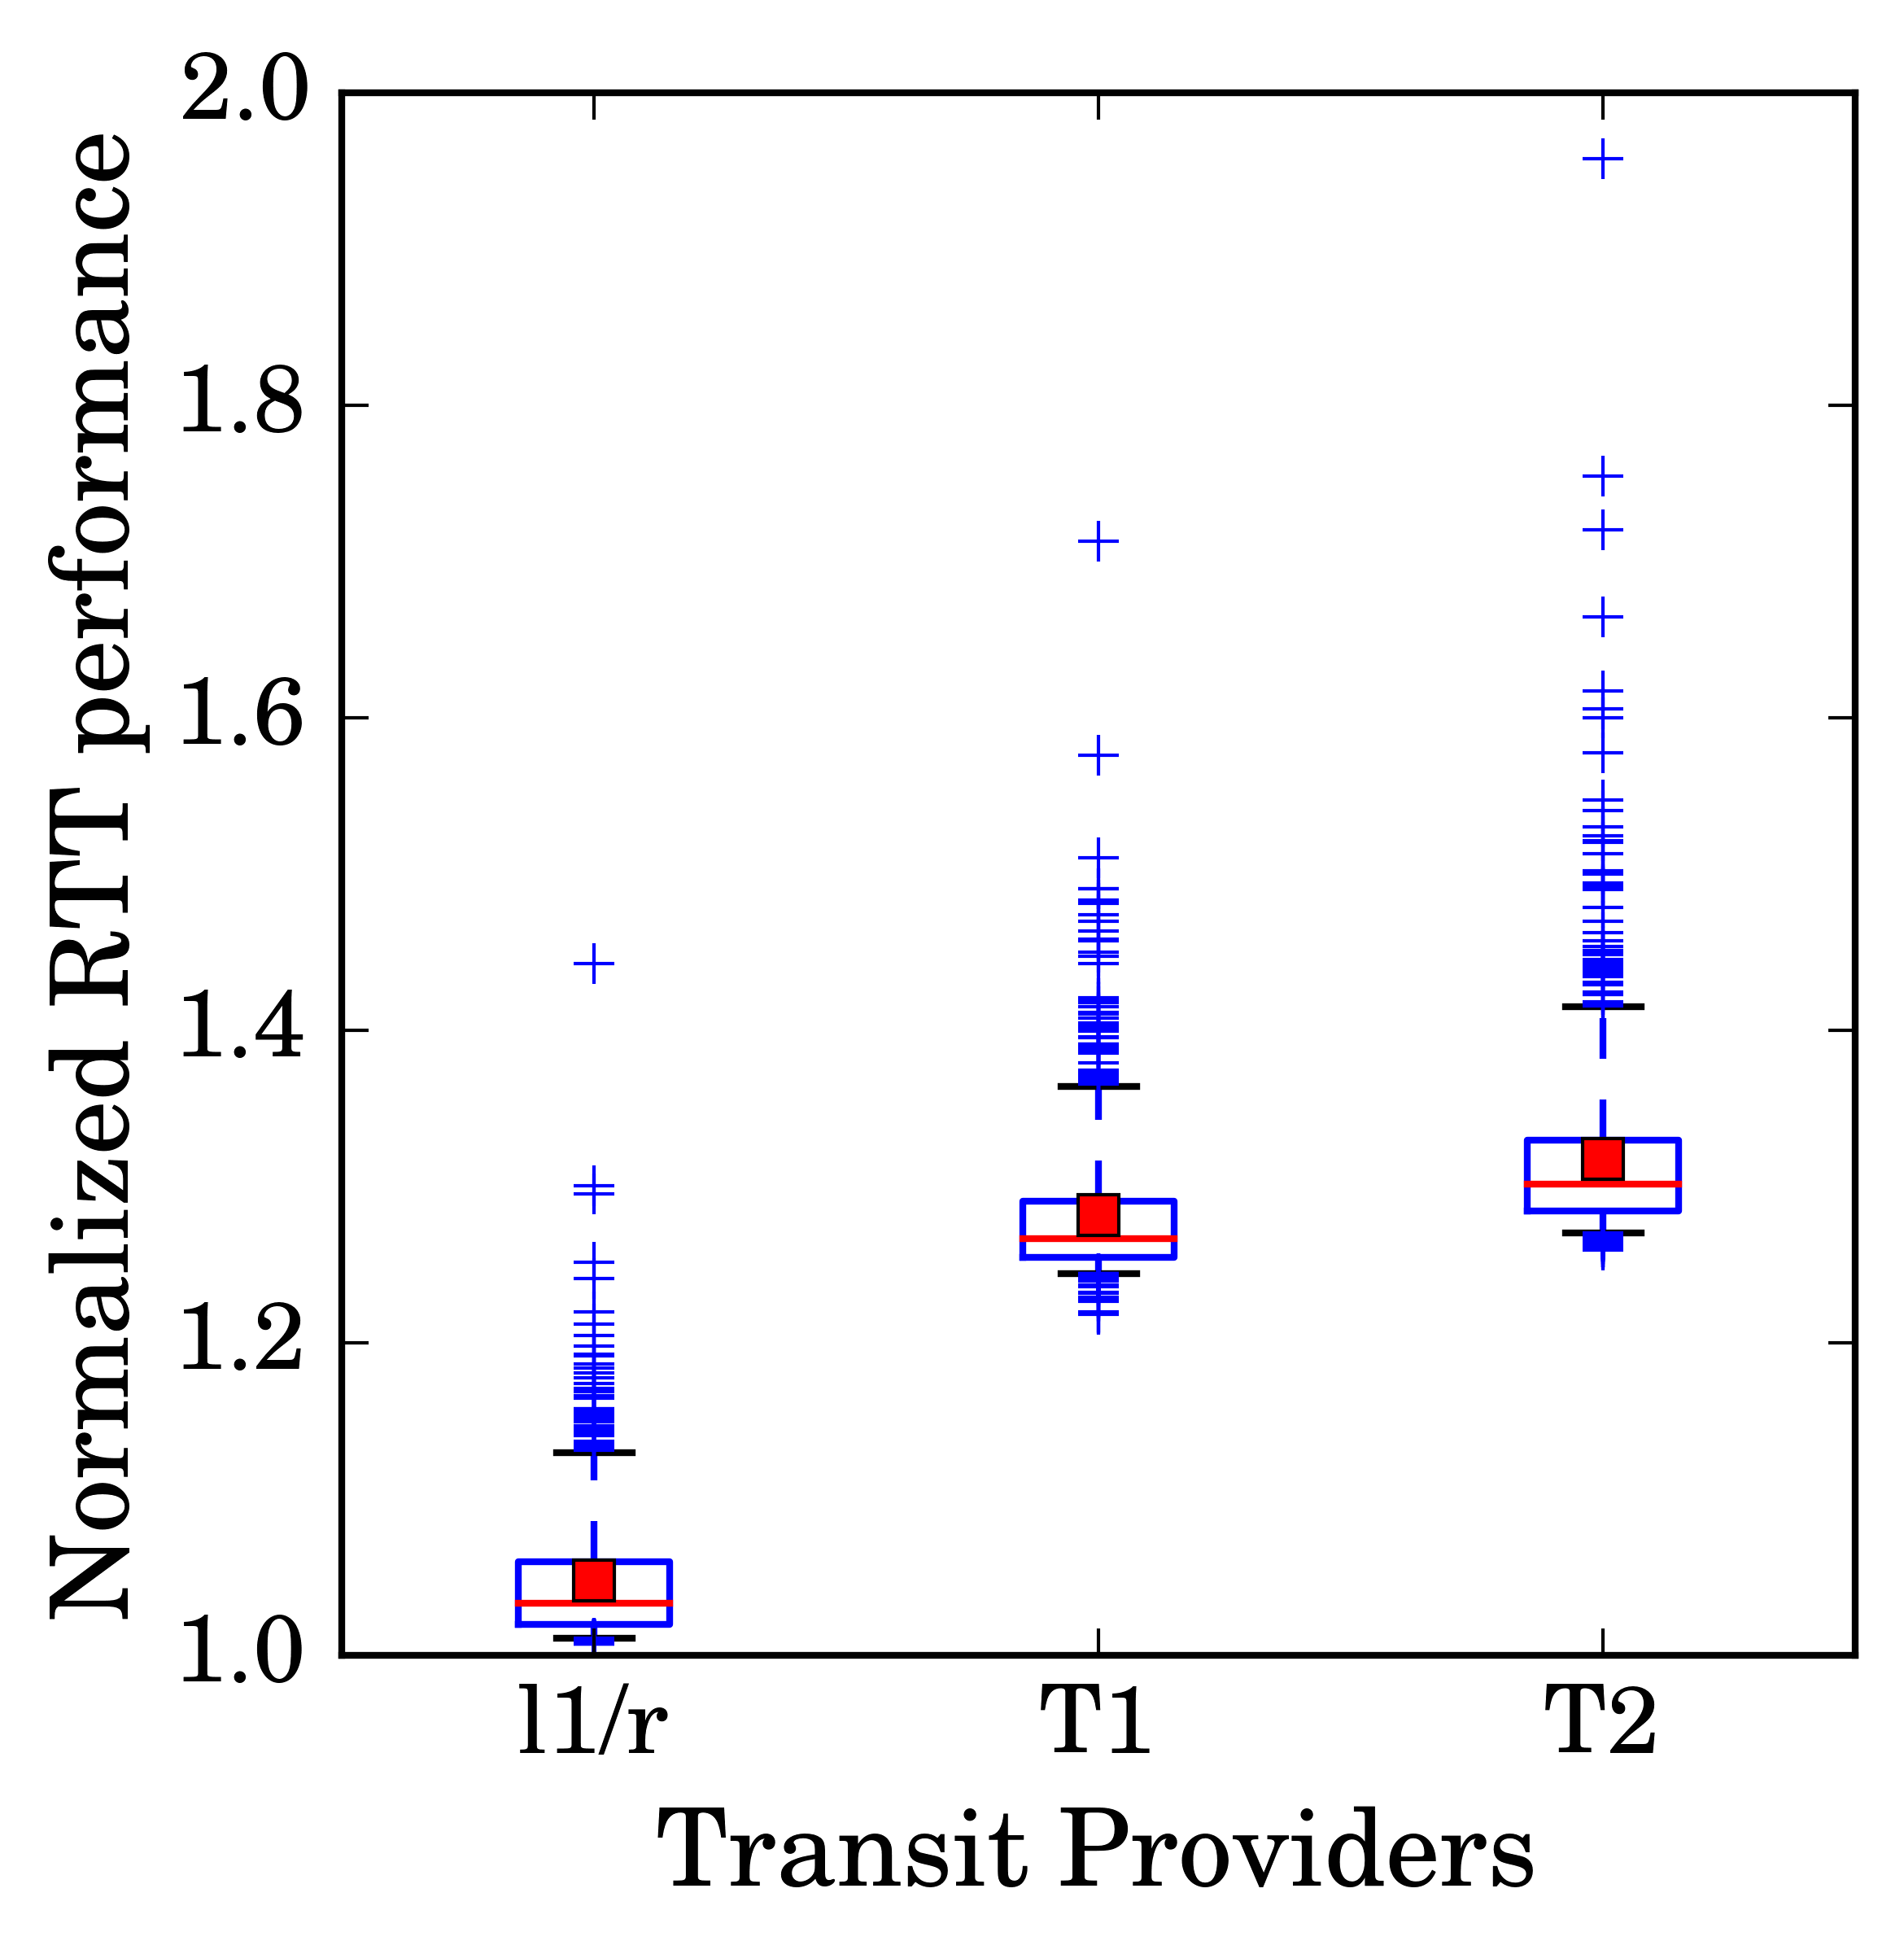
\includegraphics[width=\textwidth]{gfx/chap2/np_box_sb.png}
                \caption{SB, 935 prefixes, $48.49\%$ traffic}
                \label{fig:np_sb}
        \end{subfigure}
        \begin{subfigure}[b]{0.48\textwidth}
                \includegraphics[width=\textwidth]{gfx/chap2/np_box_sc.png}
                \caption{SC, 762 prefixes, $44.23\%$ traffic}
                \label{fig:np_sc}
        \end{subfigure}
        \begin{subfigure}[b]{0.48\textwidth}
                \includegraphics[width=\textwidth]{gfx/chap2/np_box_sd.png}
                \caption{SD, 2841 prefixes, $49.18\%$ traffic}
                \label{fig:np_sd}
        \end{subfigure}
        \begin{subfigure}[b]{0.48\textwidth}
                \includegraphics[width=\textwidth]{gfx/chap2/np_box_se.png}
                \caption{SE, 2287 prefixes, $38.59\%$ traffic}
                \label{fig:np_se}
        \end{subfigure}
        \begin{subfigure}[b]{0.48\textwidth}
                \includegraphics[width=\textwidth]{gfx/chap2/np_box_sf.png}
                \caption{SF, 879 prefixes, $78.49\%$ traffic}
                \label{fig:np_sf}
        \end{subfigure}
\caption{Normalized RTT performance with active probing. Average number of prefixes probed and average traffic volume fraction represented by these prefixes each hour are given.}
\label{fig:np}
\end{figure}
\begin{figure}\ContinuedFloat
	\centering
        \begin{subfigure}[b]{0.48\textwidth}
                \includegraphics[width=\textwidth]{gfx/chap2/np_box_sg.png}
                \caption{SG, 924 prefixes, $63.08\%$ traffic}
                \label{fig:np_sg}
        \end{subfigure}
        \begin{subfigure}[b]{0.48\textwidth}
                \includegraphics[width=\textwidth]{gfx/chap2/np_box_sh.png}
                \caption{SH, 73 prefixes, $2.83\%$ traffic}
                \label{fig:np_sh}
        \end{subfigure}
        \begin{subfigure}[b]{0.48\textwidth}
                \includegraphics[width=\textwidth]{gfx/chap2/np_box_si.png}
                \caption{SI, 642 prefixes, $67.51\%$ traffic}
                \label{fig:np_si}
        \end{subfigure}
\caption{(cont.) Normalized RTT performance with active probing. Average number of prefixes probed and average traffic volume fraction represented by these prefixes each hour are given.}
\label{fig:np_cont}
\end{figure}

In this section, we explore the potential performance gain that client networks studied in this chapter can achieve with measurement-based TE.

\marginpar{how RTT is measured}
In order to evaluate the performance gain, we continuously measured the \acf{RTT} towards selected prefixes (using $MV$ metric with $L=168$) via all available transit providers using TCP SYN scan~\cite{nmap} over the week starting from June 1st, 2015, i.e. the second week of our observation.
The probe traffic is steered by means of explicit routing.
For a pair of selected destination prefix and available transit provider, a probe is scheduled at 240 second interval in average with $30\%$ randomization in timing. 

\marginpar{how to evaluate transit performance over selected prefixes}
We quantify the performance level using certain transit provider with a metric proposed by Akella et al.\ \cite{Akella2003a}. 
This metric first normalizes the RTT via the chosen transit over the best measurement (the smallest RTT) at the same probe round. This is done for each individual selected prefix.
It then averages this normalized RTT over the entire selected prefix set.
More formally the evaluation is done as the following:
\begin{align*}
NP^{Tx}_{t_i} = \frac{1}{|SP|} \sum_{P \in SP} M^{Tx}_{t_i}(P)/\min_{T_j \in T}M^{T_j}_{t_i}(P)
\label{eq:np}
\end{align*}
where $NP^{Tx}_{t_i}$ is the normalized RTT performance for transit provider $Tx$ at probe round $t_i$, and 
$M^{Tx}_{t_i}(P)$ denotes the RTT measured toward selected prefix $P$ via $Tx$.
If a transit provider offers the smallest RTT to all selected prefixes, it should have a normalized RTT performance equaling to 1. On the other hand, a large $NP$ value indicates that the overall transmission performance  using that transit provider is far from ideal.

\marginpar{dynamic route selection as a virtual transit provider}
If the egress transit provider for real traffic is chosen dynamically for each individual selected destination prefix, the route selection mechanism can be regarded as a virtual transit provider. At each probe round, the virtual transit provider corresponds to a set of physical transit provider for each destination prefix. The set of physical provides actually employed can change over probe rounds.
We implemented a virtual transit provider, denoted as $l1/r$, first appeared in~\cite{Akella2008} for the sake of comparison. 
$l1/r$ selects the transit provider that provides the smallest RTT in last probe round for each selected prefix ($l1$ in $l1/r$). When RTT measurements data is not available (e.g. prefix newly selected, measurement timeout), it chooses randomly ($r$ in $l1/r$). This choice is based on the hypothesis that RTT of a path demonstrates temporal locality and thus is closely related to its most recent measurement.

Fig.~\ref{fig:np} gives the results of transit performance evaluation in a box-plot, where the intervals represent $5^{th}$ and $95^{th}$ percentiles (values below and beyond, marked by a \texttt{+} symbol, can be regarded as outliers).
Along the X-axis, available transit providers are aligned increasingly according to their mean normalized RTT performance (marked by a square). 

We observe that the performance differences among different transit providers is particularly evident on SC.
This confirms that multi-homing can still provide significant performance improvement nowadays. 
However this gain in performance is not inherently given in the context of BGP.
Even for transit provider that offers the best best mean $NP$, there exist moments where its performance deviates far above 1, which means that traffic toward some selected prefixes are suffering from RTTs much larger than other available transit providers.
This implies that a network can not arrive at optimal performance by using transit providers in a static and indistinguishable manner for each individual prefix.

For all networks except SG, the virtual transit provider outperforms all physical transit providers.
On SB, the performance metric $NP$ of $l1/r$ is $20\%$ lower than that of the best available transit provider.
Still, the $NP$ value of this virtual provider varies within a wide range, which calls for further investigation into the characters of RTT variation in time.

Finally, we missed RTT measurement for quite a few selected destination prefixes on some client networks, especially SH, SC, SD and SE. Reasons for such massive lack of measurement are explained in Section~\ref{sec:infer} along with a possible solution performing TE for those prefixes without measurements.

\section*{Conclusion}
\label{sec:fut}
This chapter tackled the problem of controlling a majority of data traffic via 
a small subset of BGP prefixes, by exploiting the uneven Internet traffic distribution. 
One of the challenges in addressing this problem was to select in a scalable manner the prefixes that will carry most traffic volume in the forthcoming time.  

%GgX: IMO We talk about a property of traffic, hence "volume" has to be singular.
We analyzed real traffic measurements from nine different networks located in five different countries to understand the distribution of traffic volume associated with BGP prefixes, as well as its variation in time.   
We observed that the most important prefixes (representing largest volume over a week) are generally stable in time, with small hourly variations around their mean. 
Based on our observations, we proposed three simple 
%and resource-economical   % GgX: How can a metric demand ressources? Its computation does but not the metric tiself 
metrics (also easy to compute) to proactively select prefixes with important foreseeable traffic volume.
We demonstrated that the metrics we proposed lead to better volume coverage compared to the existing solutions.
Furthermore, we evaluated the transmission performance for selected destination prefixes using different transit providers. We simulated as well a dynamic route decision algorithm. 
The results showed that with even a fairly basic mechanism, the overall RTT performance could be improved by $20\%$ compared to the best available transit provider in some networks studied. 

In order to further improve prefix selection methods, we have shown that capturing bursty prefixes is the key. 
To this end, we could group prefixes by their activity profiles. 
For each group, selection method is adapted to its traffic dynamism.
When dealing with prefixes with regular volume patterns and small hourly variation, the simple metrics proposed in this work perform already sufficiently well. 
Nevertheless, for bursty prefixes, we might need a more sophisticate model that extracts additional activity features, for instance long term periodicity.
The burstiness index $\beta$ proposed in this chapter, shown to be very expressive, could be potentially used in prefix characterization and classification and thus is worthy of future work.
\cleardoublepage
\chapter{Internet measurement with RIPE Atlas}
\label{sec:ripe_atlas}
\section*{Abstract}
Starting from this chapter, the center of our study is oriented to delay and path measurements, and how to make use of them in measurement-based interdomain \ac{TE}.
Same as volume statistics studied in Chapter~\ref{sec:pref_selec}, these measurements are readily available on client TE platforms.
However, we decided to switch to measurements conducted by RIPE Atlas, a measurement platform offering open data access to public, for the sake of reproducibility.

This decision is justified through a brief analysis on the elements of reproducibility and how RIPE Atlas satisfies them in design.
To facilitate the discussion in later chapter concerning measurement collection, we introduce succinctly the building blocks of RIPE Atlas, its measurement methods and how a particular measurement can be identified and retrieved.

RIPE Atlas is a great facilitator for a better understanding of the Internet, yet it is not without out problems. We study the potential data quality issues stemmed from the platform itself, particularly missing measurements. We verified whether missing measurements were due to prone disconnection from the controller.
Unexpected probe behavior is discovered, analyzed and reported to the RIPE Atlas engineering team, in hopes of contributing to the RIPE Atlas community.

Further, we study as well data quality concern specific to measurement-based TE: does the RTT measurements mainly reflect the AS path level network characteristics?
In order to shed light on this issue, we explore the inherent structure of a data set composed of 100 RTT time series measuring a same AS path through clustering.
Results showcase that a part of these RTT measurements were subject to access network congestion that can not be avoided with interdomain TE. This finding confirms the need for data cleaning, a process often neglected in previous practices.

At the end of this chapter, we present a case study on multiple RTT time series undergoing a similar shape RTT change at about the same moment. The presence of such case can potentially help reveal where does the change comes from, thus having important implication in TE as well as for a better understanding of the Internet. We tentatively employ time-series clustering methods to group RTT time series with similar shape together.
\clearpage

\section{Reproducibility}
\marginpar{Issue with previous dataset.}
We collected traffic volume and delay data from real client networks in Section~\ref{sec:pref_selec} and developed all the studies concerning prefix selection on that dataset.
Having access to real client data increases the credibility of the discoveries made in the study, and enhances the relevance of proposed schemes basing on these findings.
The other side of coin is that such private dataset hinder the reproducibility, a paramount feature in metrology researches.

\marginpar{What we talk about when we talk about reproducibility?}
The \acf{ACM} offers definition for various terms referring to different degrees of research repoducibility~\cite{acm}, ranging from repeating the same result by the same team to reproducing the same result with independent implementation of proposed methods or measurement system.
The way the measurement data is generated, stored and accessed is one of the key elements for all these degrees of reproducibility.

\marginpar{data generation}
Previous data from client network comes from measurements performed by proprietary commercial platforms~\cite{b6}.
By nature, it is against the fundamental benefit of the company to reveal the technical details on how measurements are done. Even permission of disclosure granted, we as research more often than not do not have enough space to include such technical details in publication.

\marginpar{data storage}
Since the collected data contain sensible information, e.g. the destination prefixes clients talked to, client IP addressing schemes, transit provider choices etc., they are required to remain on client owned platforms otherwise permission required. Due to capacity limitation and decreasing utility of old data, these measurements will not stay forever available on client servers. If measurements are allowed to be retrieved, we as researchers are then responsible for the storage of these data. Server clusters in research institution may offer temporary (available till graduation) storage infrastructure, yet researchers are responsible for the security of these data. Once data compromised, researchers may face serious legal consequences.

\marginpar{access to data}
Due to the sensitivity nature of data collected from client platforms, direct open access to the research community/public is not an option. Data anonymization is required. The process is not trivial as an appropriate balance is hard to hit. If not enough, some features of the client data can still be deduced and subject to unwanted exposure. If too much, the interpretation based on the anonymized data could become obscure and lack of credibility. Moreover, for better representativeness and statistical confidence, Internet measurement researches stress on large dataset over long period. This inevitably increases the size of dataset. Maintaining the access to these large dataset is clearly not without cost. However current publication reviewing process provides limited support on submitting voluminous supporting material without breaking the identity author/review anonymity~\cite{bajpai2017challenges}.

Bearing these considerations in mind, we look for measurement platforms alleviate the burden in measurement execution, storage and public access.

\section{RIPE Atlas for reproducibility}
RIPE Atlas is not the only Internet measurement platform that provides open data access~\cite{Bajpai2015}.
We justify this choice by first introducing RIPE Atlas. Then we summarize and highlight its features that qualify it as the best option for our research with comparison to alternative measurement platforms.

\subsection{Overview of RIPE Atlas}
\begin{figure}[!htb]
\centering
\includegraphics[width=\textwidth]{gfx/chap3/ripe_atlas_archi.pdf}
\caption{Building blocks of RIPE Atlas.}
\label{fig:ripe_atlas_archi}
\end{figure}

\acf{RIPE} Atlas is a measurement platform centrally managed by the European Internet register.
Fig.~\ref{fig:ripe_atlas_archi} sketches the architecture of the platform.
Probe are dedicated devices from which measurements are launched.
The operation system on the probes are tailored by RIPE engineers for Internet measurements~\cite{firmware}.
These probes are distributed either by RIPE or by RIPE Atlas Ambassador~\cite{ambassador} upon demand from anyone willing to host the probe and keep it online in his network.
As of this writing (July 11, 2017), 19448 probes have been sent out and 9854 of them remain active.
All these probes, hosted in 3511 IPv4 ASes and 1286 IPv6 ASes across 181 countries, can be commanded by a single platform user to measure any destination in the Internet.

As a platform user, one does not have to connect to all these probe by him/herself to 1) create specific measurements; 2) fetch measurement results. 
One only has to interface with RIPE to fulfill the above essential tasks along with other helpful functions such as measurement data visualization.
To that end, RIPE collects in quasi-realtime measurements from all the connected probes and stores them in its server clusters. Programming API~\cite{atlasapi} as well as human friendly Web sites are developed to facilitate the data operation of all kinds.

\subsection{Measurement types}
It is though not possible to run user specified measurement tools, e.g. nmnap~\cite{nmap}, scamper~\cite{luckie2010scamper} or bandwidth measurement tools, RIPE Atlas does support a wide range of standardized Internet measurements with configurable parameters: ping, traceroute, DNS, SSL.
Ping and traceroute measurement offer the Internet delay and path information required in measurement-based TE.

Another way of classifying the measurements is via the entity of measurement creator. As shown Fig.~\ref{fig:ripe_atlas_archi}, user of the platform (does not necessarily host probes) enjoys a great degree of 
liberty of specifying the destination and sources of supported measurements. These are \acf{UDM}. Once a user defines a measurement, the central controller clusters schedules it to corresponding probes and collects the results once the measurements started.
On the other hand, there exist another category of measurements defined by RIPE itself call built-in measurements~\cite{atlas}. These measurements are automatically executed by the probes themselves, with out need for controller commands. These measurements, originated from all probes, are mainly ping, traceroute and DNS measurements to DNS root servers and RIPE infrastructures.
In the later studies, we heavily rely on these built-in measurements given their world-wide footprint, super long history records (date back to the day one of each probe) and low additional measurement costs.

\subsection{Describe, identify and fetch measurements}
Besides measurement type specific parameters, such as the protocol type for traceroute, following three elements are as well fundamental describing a RIPE Atlas measurement: 1) participant probes; 2) the single measurement destination per measurement; 3) the time span of the measurement. 

Once a \ac{UDM} is created, it can be identified by an unique measurement ID. 
Each built-in measurement can as well be identified with a pre-assigned ID.
It is with this measurement ID, one learns the description, accesses data visualization provided by RIPE and eventually fetches the raw measurement results.
For example, with \url{https://atlas.ripe.net/measurements/3742863/#!openipmap}, one can have access to the path visualization of measurement $\#3742863$, where 100 probes word-wide are selected to perform one-time traceroute toward \url{www.sigcomm.org}. With \url{https://atlas.ripe.net/api/v2/measurements/3742863/results/?start=1462147200&stop=1462233599&format=json}, anyone can easily download the entire raw measurement records of this measurement.

\subsection{Advantages}
RIPE Atlas is a measurement platform designed to facilitate reproducible researches. RIPE take care of all the engineering challenges of 1) measurements execution from geographically distributed probes; 2) reliable and continuous data storage; 3) public access to data; 4) simple syntax for describing, identifying measurements; 5) well documented open-source programming tools for data manipulation.

The advantages of RIPE Atlas go beyond reproducibility. Compared to perfSONAR, PlanetLab and DIMES, probes of RIPE Atlas, with dedicated hardware for measurement task, are supposed to deliver measurements that better reflect the network character and are less impacted by probe local resource sharing issues~\footnote{perfSONAR: ~\url{https://www.perfsonar.net}; PlanetLab:~\url{https://www.planet-lab.org}; DIMES:~\url{http://www.netdimes.org}}.
Moreover, RIPE Atlas rapidly is gaining popularity among many non-academic networks, such as \ac{ISP}, \ac{CP} and \ac{IXP}, thanks to a wide range of monitoring applications hence enabled, to name a few, performance monitoring~\cite{latencymon, Rimondini2014}, anomalies detection~\cite{Fontugne2016, Padmanabhan, halo}, peering and IXP measurements~\cite{ixp, routeixp} etc. Increasing number of commercial networks host RIPE Atlas probes or anchors (a more powerful version of normal probe),   providing a much richer and realistic network profile from which measurements can be initiated, compared to other alternative options.

\section{Measurement quality}
We dedicate the discussion of this section to data quality, another key issue to metrology researches besides reproducibility. To begin with, we show that it is common to lose some datapoints for measurements scheduled at regular interval on RIPE Atlas. The temporal correlation between missing measurements and connection events are 
analyzed, in the pursuit of understanding reasons behind such missings.
To our surprise, a big part of measurements are lost while probes are connected.

Later on, with the RTT measurements from RIPE Atlas, we explore a data quality issue specific to interdomain TE. It deals with the fact that multiple measurements (potentially with different IP paths) could exist to quantify the transmission performance between two ASes. Are these measurements all alike? Which ones shall we use to make TE decisions?

\subsection{Missing measurements on RIPE Atlas}
\label{sec:miss_atlas}
Through previous studies~\cite{Holterbach2015a, Bajpai2015}, it is now known that load have obvious impacts on measurement precision and scheduling.
We focus on data completeness, another aspect of measurement quality that received less attention so far. Missing measurements can cause various undesired consequences. Apart from widening confidence interval of inference~\cite{Fontugne2016}, it requires in general methodological adaptations, e.g. in spectrum analysis~\cite{Babu2010, Luckie2014, shao2016}, otherwise biased estimation would be expected~\cite{Baraldi2010}.
%Therefore it is of relevance to question the nature of missing measurements.

One obvious reason of missing is that the probe is not running (properly), e.g. power off~\cite{schedule}.
As long as a probe is powered, it tries to maintain a connection to a controller to report measurements and receive assignments as shown in Fig.~\ref{fig:ripe_atlas_archi}. 
Therefore the probe connection activity provides a good indication of the probe availability, and is used in current investigation conducted by RIPE on probe OS stability~\cite{1look, 2look, 3look}.

In order to infer other possible causes, we compared the measurement timestamps with the moments probe connects to and disconnects from a Atlas controller.
If measurement missing coincides with the probe disconnection, chances are that the probe is dysfunctional during the missing. However, if measurements are lost while the probe is well connected, something `abnormal' should be expected, beyond the known probe OS issue.

\subsubsection{Data collection}
We observed the RIPE Atlas platform for one month, from 2016-06-01 to 2016-07-01 UTC.
All the v3 probes first connected before the beginning date (11613 of them) are considered.
Connection events (measurement ID 7000) and built-in Ping measurements to DNS b-root (measurement ID 1010), a highly available destination, are collected~\cite{built-in}. 
Controllers and the ping destination are not within the same network.
Controller logs the moments at which probes connects to and disconnects from it.
The built-in ping measurement is scheduled on every probe at 4min interval. 
10800 ping results are thus expected from each probe within the month.
7353 probes, out of the available 11613, had Ping measurements during this period.

\subsubsection{Missing at first glance}
\begin{figure}
\centering
\includegraphics[width=0.7\textwidth]{gfx/chap3/missing_length_cdf.pdf}
\caption{CDF of total missing length per probe.}
\label{fig:miss_len}
\end{figure}
We deem that there are missing measurements when the time interval between two neighbouring measurement are much longer than the planned value. 
Such long gaps turn out to be very close to integer times of planned interval, as a cron-like mechanism is used to run measurements at regular interval and it retakes the previous phase after interruption~\cite{source, schedule}.
This character allows quantifying the length of missing segment by the number of measurements skipped.
4440 probes  (60.4\%) miss no more than 2 datapoints, which is totally legitimate, as random jitter is added to each single measurement to avoid synchronization among probes.
For the rest, the missing length spans a wide range according to Fig.~\ref{fig:miss_len}.
1358 (18.5\%) probes miss more than 10\% of the total measurements (i.e. 72 hours over a month).

\subsubsection{Cross missing measurement with connection events}

\begin{figure}[!htb]
\centering
\includegraphics[width=0.6\textwidth]{gfx/chap3/len_by_ratio.pdf}
\caption{Missing length distribution.}
\label{fig:len_ratio}
\end{figure}

\marginpar{missing overlapped with connected period}
Several reasons may contribute to the disconnection of a probe to its controller: 1) probe not working (properly); 2) network issues preventing the connection; 3) controller not available, e.g. during maintenance~\cite{controller}. Meanwhile, the last two reasons shall not prevent a probe from performing built-in measurements, as the results can be unreachable or timeout, and be stored locally on the probe~\cite{usb}. 
That is to say, \textit{missing does not necessarily occur when probe is disconnected, but is unexpected while probe is connected.}

We count, for each missing segment, the number of missing measurements that occurred during a connected period.
We obtain the \textit{overlap ratio} by dividing this count by the length of missing segments. 
The distribution of overlap ratio is concentrated at the two ends, 0 and 1. 
For the convenience of illustration, we cut missing segments into two groups, one with overlap ratio $\leq0.5$, denoted as \textit{shifted}, the other with the rest, denoted as \textit{overlapped}.
Measurement missing that overlaps connected period is `unexpected'.

The two groups demonstrate different length distribution profiles, Fig.~\ref{fig:len_ratio}.
15391 missing segments are observed. 
10292 (66.87\%) missing segments are overlapped with connected period. 
They are mostly short in length. 5560 of them last no more than 2 measurements. 
One possible explanation is that these measurements are skipped due to scheduling or load issues~\cite{schedule, Holterbach2015a}.
Meanwhile, 2490 of them are equal to or longer than 1 hour, involving only 620 probes, for which we believe that the previous explanation hardly applies.
%% 620 probes ever have long overlapped missing segments, relatively a small portion.

Missing segments shifted from connected period are more likely to be long. This is possibly due to the v3 probe OS stability issue still under investigation. It is known to be responsible for long term probe disconnection and requires manual operation to recover the probe~\cite{usb, 1look, 2look, 3look}.

\begin{figure}[!htb]
\centering
\includegraphics[width=0.98\textwidth]{gfx/chap3/all.pdf}
\caption{(D/C, C) stands for missing segments more closely correlated with disconnected period.
Number of concerned missing segments is given in the title. Negative time distance means the edge happens before the connection event and vice verse.}
\label{fig:all}
\end{figure}

\marginpar{temporal correlation between missing and connection events}
To obtain a subtler view, we seek to find out: when do measurements begin to be lost and when are they recovered? Are these moments close to connection events?

First, we define the \textit{left edge} as the last measurement before a period of measurement absence, and the \textit{right edge}, accordingly, the first measurement after recovery. 
We then calculate the time interval separating these edges and the closest connection events. We also identify the nature of these events, and mark `D/C' for disconnection, `C' for connection. 

1284 missing segments locate at the beginning or the end of the observation period. 
They are unavailable for this analysis as only one edge can be observed.
For the rest with both edges, 5793 missing segments' left edge is closer to a disconnection event and the right edge is closer to a connection event, according to Fig.~\ref{fig:all} sub-graph (D/C, C).
Judging from the density contour, last measurement most likely precedes disconnection by a Ping interval (4min), and recovery tends to take place 4 minute after the connection.
Such strong correlation with probe disconnected period indicates that probe dysfunction is probably the cause.

However, the beginning of such missing segments (D/C, C) can as well be dislocated from disconnection event.
At the left end of the graph, measurements are lost long before the disconnection, which we find `abnormal', even though the recovery is near connection.

To the right end, measurements only begin to be lost a long time after the probe is disconnected. One possible explanation is that measurements are first stored locally after disconnection from controller~\cite{usb}. Then new measurements are lost after local storage is full.

Contrary to the compact distribution in (D/C, C) sub-graph, the majority of the rest missing segments spreads along the time axis. 
The distances from left and right edge to connection events are highly correlated, suggesting that both left and right edges are on the same side of a same connection event.
We note that these measurements were mostly lost while probes were well connected, i.e. overlapped.

\subsubsection*{Wrap-up}
In our analysis covering a large number of probes over one month, only 60\% of v3 Atlas probes have complete measurements. Around $1/3$ missing segments appear to closely correlated to disconnected period. The probe OS stability issue might have contributed to such missings, as suggested by the heavy tail of the missing lengths.

However, the remaining $2/3$ of missings occurred while probes are connected. 
Half of them are no more than 2 measurements in length, and are thus likely to be caused by scheduling issues. However, around $25\%$ of this category lasts long($\geq 1h$). 
We reported the discovery to RIPE engineering team along with a specific case that they could started with.
The last reply from RIPE team confirmed  that the probe we mentioned in report had ``time synchronization issues''. To help advance the investigation, we share with RIPE team all the long missing segments identified. These exchanges can be found on the RIPE Atlas forum at \url{https://www.ripe.net/participate/mail/forum/ripe-atlas}, with tile ``Actual measurement interval much larger than planned''.

\subsection{Same AS path measured by different probes}
Whether the measured RTT mainly reflects the network characteristics of AS paths traversed real traffic is a data quality concern specific in the context of measurement-based interdomain TE.
It is simply because route selection function in Fig.~\ref{fig:archi} relies on path performance measurements as input, more details in Chapter~\ref{sec:cpt_rtt}.
However, RTT measurements might be `polluted' either by non-network factors, say host-local issues as CPU overload, or non-representative sub-AS level network issues can not be optimized with interdomain TE, say local congestion along the ASes traversed. 
However, none of these previous works~\cite{Goldenberg2004, Akella2008} on measurement based inter-domian TE has realized the importance of this problem.

This data quality issue gives rise to a series of questions: if we measure over a period of time a same AS path with multiple different RTT measurements toward different hosts in the destination AS, what will these RTT time series look like? Will they have similar characters? If not, how can we pick out the ones fit best for our TE uses?
We try to answer to these question by performing clustering over a such set of RTT time series, in the purpose of automatically revealing their inherent structures.

\subsubsection{Data collection}
We emulated such RTT measurements between two ASes, the local client AS (one host) and one destination AS (multiple hosts) with RIPE Atlas built-in measurements $\#1006$ and $\#5006$.
They are respectively IPv4 ping and traceroute measurements from all Atals probes to m.root-servers.net (202.12.27.33). 
Ping measurement is scheduled at 240sec interval, while traceroute at 1800sec.
120 RIPE Atlas probes within AS3215 are selected to construct our database.\footnote{The 120 probes are the same ones in user-defined measurement \#2427397 with open access to all.}
We assumed that all probes hit the same DNS root server clusters as the AS-level path toward the destination (m-root) is the same, since the only upstream AS for AS3215 is AS5511, the backbone of a French \ac{ISP}. Time window for the data collection ranges from 2015-09-28 10:00:00 UTC to 2015-09-29 12:00:00 UTC.

We cleaned the data collected, with following steps:
\begin{itemize}
\item Remove probes with unstable connection to the Atlas platform. (Short total length, multiple missing segments~\ref{sec:miss_atlas});
\item Remove probes suffering from obvious hardware or local network issues. (high packet loss, or error flag found in measurement results).
\end{itemize}

We then consider only 100 common probes in both ping and trace traces remained after cleaning.
All valid probes considered, the average hop number to the destination, m-root server, is 9. 
For the traceroute data set, we decided to concentrate on the first 3 hops (which should represent the access network). As a consequence, the traceroute data set are further cut into 3 parts, where each contains the RTT time-series till the corresponding hop.

To sum up, we fabricated four RTT time series data sets, on which we performed time series clustering:
\begin{itemize}
\item \texttt{pingData}, end-to-end RTT time series;
\item \texttt{traceData1}, RTT series till the first hop;
\item \texttt{traceData2}, RTT series till the second hop;
\item \texttt{traceData3}, RTT series till the third hop;
\end{itemize}

\subsubsection{Clustering RTT series in feature space}
\label{sec:cls_ft}
Generally speaking, a time series clustering approach can be decomposed into three parts: data representation, distance measure and clustering algorithm~\cite{Aghabozorgi2015}. 
Due to its high dimension, time series is seldom used in its raw form, whence data representation.
Common approaches include dimension reduction~\cite{Elhamifar2013}, pattern extraction~\cite{Ulanova2015}, etc.
Distance measure quantifies the similarity/dissimilarity of two time series. Finally, clustering algorithm defines the procedure of grouping time series based the distances calculated on their data representation space.
For each of these components, multiple possibilities exist. However, it is not clear which one and which combinations of them could be the best fit to RTT measurements. 

\marginpar{data representation adopted}
In this section, we extracted a set of features listed below from each individual time-series and used in actual clustering. 
The advantage of such data representation is that it first largely reduces the data dimension. Thanks to that, data set is more suitable to classic partitioning clustering methods, like k-means and k-medoids (also known as PAM, partitioning around medoids)~\cite{Lin2003}.
Second, it is able to depict the data set from multiple aspects that are not evident with the raw form. 
%However, the clustering results could be biased by the selection of features.
Before clustering, each feature is z-normalized (zero mean and unit variance).
%so that result is not biased towards features with big value and high variance.
%%% At last I understood !!! Eureka. 

Following features are used in this work:
\begin{description}
\item[Power spectral density] is calculated using PyEgg~\cite{Bao2011} and cut into three bins, $(0, 1/12], (1/12, 1/6]$ and $(1/6, 1/2]$ of measurement frequency. Each of the bins individually functions as a feature.
\item[Sampling Entropy] proposed by Richman and Moorman~\cite{Richman2000} quantifies the regularity or predictability of a time series. In calculation~\cite{Bao2011}, we used an embed dimension of 2 and a tolerance of 15 msec.
\item[Number of changes] counts the number of times where the difference between two consecutive RTT measurements is greater than 15msec. %We did not use change detection methods that adapt to mean and deviation level of a window in the past, e.g. those based on z-score, for we assert that an absolute RTT change more than 15msec is significant, regardless of the mean and $std$ of an RTT trace. 
\item[Range] is the difference between the maximum and the minimum values of an RTT series.
\item[Mode] is the value most frequently present in a time-series.
\item[Mean], the first-order moment, describes the overall RTT level.
\item[Standard deviation] is derived from the second-order moment, describes how close measurements are to the mean.
\item[Skewness], the third-order moment, describes the lack of symmetry of RTT values observed around the center point of histogram, mode.
\item[Kurtosis], the fourth-order moment, describes whether the histogram of observations are peaked or flat relative to a normal distribution.
\end{description}
With RTT time series represented in the above feature space, we simply use \acf{ED} to measure the distance between two RTT time series.

\iffalse
\begin{figure}[!htb]
    \centering
    \begin{subfigure}[b]{.7\textwidth}
	\includegraphics[width=\textwidth]{gfx/chap3/pingSil.pdf}
	\caption{\scriptsize \texttt{pingData}}
	\label{fig:pingSil}
	\end{subfigure}
	\begin{subfigure}[b]{.7\textwidth}
	\includegraphics[width=\textwidth]{gfx/chap3/traceSil1.pdf}
	\caption{\scriptsize \texttt{traceData1}}
	\label{fig:traceSil1}
	\end{subfigure}
	\begin{subfigure}[b]{.7\textwidth}
	\includegraphics[width=\textwidth]{gfx/chap3/traceSil2.pdf}
	\caption{\scriptsize \texttt{traceData2}}
	\label{fig:traceSil2}
	\end{subfigure}
	\begin{subfigure}[b]{.7\textwidth}
	\includegraphics[width=\textwidth]{gfx/chap3/traceSil3.pdf}
	\caption{\scriptsize \texttt{traceData3}}
	\label{fig:traceSil3}
	\end{subfigure}
\caption{ASW (Average Silhouette Width) using different clustering algorithms when varying number of clusters.}
\label{fig:sil}
\end{figure}
\fi

\begin{figure}[!htb]
\centering
\includegraphics[width=.7\textwidth]{gfx/chap3/pingSil.pdf}
\caption{\ac{ASW} achieved on \texttt{PingData} using different clustering algorithms when varying number of clusters.}
\label{fig:pingSil}
\end{figure}

\marginpar{Which cluster method is the most appropriate?}
Several clustering algorithms are available. 
In order to choose the one that fits best to our data set and decide the most appropriate cluster number, we use \acf{ASW}~\cite{Rousseeuw1987} to evaluate the quality of resulted clusters. 
It takes value in the range of $[-1,1]$. 
\ac{ASW} of a certain achieved cluster is a measure of how tightly all the data in the cluster are grouped together. 
While the \ac{ASW} over the entire dataset, is a measure of how appropriately the data has been clustered. For a single clustering method, we can find out what is the cluster number k that this algorithm is most confident of by picking the k offering the biggest \ac{ASW}. Across two different clustering algorithms, we could tell which one performs better by comparing the \ac{ASW} of resulted clusters, i.e. a better clustering result shall have a bigger \ac{ASW} value.

Following clustering algorithms are tested: hierarchical clustering with Ward linkage, k-means, \ac{PAM}.
Dataset-wide \ac{ASW} are visualized in Fig.~\ref{fig:pingSil}. We can see that for \texttt{PingData}, k-means algorithm with $k=2$ offers relatively confident clustering results. 
This observation holds as well true for traceroute data sets.
Hence, such settings are used in the rest of the work.


\subsubsection{Clustering result interpretation}

\begin{table}[!htb]
\centering
\footnotesize
\setlength{\tabcolsep}{0.5em}
\begin{tabular}{l|ccc|ccc|ccc|ccc}
\toprule
\multirow{2}{*}{\# cls} & \multicolumn{3}{c|}{\texttt{pingData}} & \multicolumn{3}{c|}{\texttt{traceData1}} & \multicolumn{3}{c|}{\texttt{traceData2}} & \multicolumn{3}{c}{\texttt{traceData3}}\\
& size & dist. & AWS & size & dist. & AWS & size & dist. & AWS & size& dist. & AWS\\
\midrule
1 & 25 & 4.37 & 0.23 & 93 & 3.98 & -0.21 & 76 & 3.02 & 0.41 & 31 & 4.35 & 0.07\\
2 & 75 & 2.61 & 0.54 & 7  & 2.17 & 0.35  & 24 & 4.58 & 0.08 & 69 & 2.90 & 0.41\\ 
\midrule
AWS &\multicolumn{3}{c|}{0.46} & \multicolumn{3}{c|}{-0.17} & \multicolumn{3}{c|}{0.33} & \multicolumn{3}{c}{0.30}\\
\bottomrule
\end{tabular}
\caption{Summary of clusters characters on \texttt{PingData} feature space. Clusters are achieved from each corresponding dataset, while the statistics of clusters are computed with \texttt{PingData}.}
\label{tab:summary_cls}
\end{table}

\marginpar{How the two clusters are different from each other?}
Table~\ref{tab:summary_cls} provides several metrics describing the achieved clusters: size of cluster, intra-cluster distance, intra-cluster \ac{ASW}, and overall dataset-wide \ac{ASW} at the bottom.
Focusing on the column for \texttt{PingData}, we notice that two clusters of unbalanced size are obtained.
Cluster 2 is much larger in size, yet with smaller intra-cluster distance. 
In accordance, the cluster algorithm is more confident of this cluster than the other, as the cluster \ac{ASW} is much higher.
This indicates that the members within cluster 2 demonstrate strong common features and are thus more closely placed to each other in the feature space.

\begin{figure}[!htb]
\centering
\includegraphics[width=.6\textwidth]{gfx/chap3/ping_pca_ping.pdf}
\caption{Projections of clusters on \ac{PCA} features, \texttt{PingData}.}
\label{fig:ping_pca}
\end{figure}

\marginpar{view from \ac{PCA} surface}
This ``guess'' can be straightforwardly observed from the projection of clusters on \acf{PCA} surface, shown in Fig.~\ref{fig:ping_pca}.
The contribution of each feature is as well indicated on the graph.
We notice that most of these points to different directions on the \ac{PCA} surface, suggesting that they are a comprehensive yet concise description of the date set.
As a consequence, no single feature takes dominant position in forming the clusters.
Still, tendency is that cluster 2 includes data points with little  changes, small entropy and small standard deviation. 

\begin{figure}[!htb]
    \centering
    \begin{subfigure}[b]{\textwidth}
	\includegraphics[width=\textwidth]{gfx/chap3/rtt3d_ping_cls1.pdf}
	\caption{cluster 1.}
	\label{fig:ping_cls1}
	\end{subfigure}
	\begin{subfigure}[b]{\textwidth}
	\includegraphics[width=\textwidth]{gfx/chap3/rtt3d_ping_cls2.pdf}
	\caption{cluster 2.}
	\label{fig:ping_cls2}
	\end{subfigure}
\caption{End-to-end RTT series of cluster members from \texttt{pingData} dataset.}
\label{fig:rtt_ping}
\end{figure}

\marginpar{view from RTT time series}
Fig.~\ref{fig:rtt_ping} plots the RTT time series of these two clusters. Cluster 2, as expected, contains mainly traces with only a few variations and spikes. 
On the other hand, cluster 1 is composed of traces with large variations.
This explains why the members of cluster 2 are more closely located to each other. 
It is because for a time-series to be smooth, there is only one form, while for it to be full of variations, there could be many possibilities.
%Let's also note that for smooth time-series (cluster 2), there is only one form, 
%while many different possible shapes can be observed in the other cluster.

\begin{figure}[!htb]
\centering
\includegraphics[width=\textwidth]{gfx/chap3/rtt3d_ft_pam_cls8.pdf}
\caption{One cluster achieved when $k=12$, \texttt{PingData}.}
\label{fig:cls8_k12}
\end{figure}

\marginpar{advantage of clustering with multiple features}
What is also worthy of noticing is that cluster 2 actually tolerates traces with a few spikes and variation of small amplitude. 
This is due to the advantage of using clustering instead of ranking with one single feature, which would also be viable to isolate ``noisy'' traces. 
For instance, we could rank the RTT traces by their entropy and assume top x traces are ``noisy'' ones. 
The shorting-coming of such approach is two-fold.
First, single feature might ``wrongly'' rank certain RTT time series. 
For example, entropy~\cite{Molina-Pico2011} and power spectral density are very sensitive to spikes. 
In networking uses, we believe that one or a few spikes in an RTT measurement shall not deteriorate an entire trace. 
Second, one has to define threshold values to deliberately separate data set into two or more parts. 
While with clustering, multiple features can be considered at same time. 
Plus, the most appropriate number of clusters changes automatically with the input and reveals the inherent structure of the data set. 
By setting a larger cluster number, one could achieve more fine-grained clustering results that convey subtler information. An example is given in Fig.~\ref{fig:cls8_k12}, where several traces of similar variation shape is grouped together.

\marginpar{interpretation in the context of interdomain TE}
The two clusters achieved are as well of relevance in interdomain TE. 
It shows that when measuring an AS-level path by probing multiple hosts in destination network, resulted RTT time series can take very different shapes. 
One possible explication is that the IP-level path toward certain hosts suffers from local problems.
If certain RTT variation is due to congestion on an inter-AS link, then it shall be shared by all the RTT time-series. If not shared, such RTT variation is probably related to local issues can not be avoided by changing an egress transit provider in sending out the traffic.
Therefore, when comparing multiple RTT time series between two ASes, the ones with fewer variations are supposed to be less impacted by these local conditions and give a more faithful view on the AS-level path performance.
One another advantage of using smoother RTT time series in choosing egress transit, is that resulted routes is supposed to be more stable. Fewer variations would actually trigger fewer route changes. 

\marginpar{take-away}
To summarize, when clustering RTT time-series in feature space, no specific assumption is imposed by the extracted features, yet we arrive at two clusters that tell noisy traces apart from smooth ones.
This reveals the inherent structure of the data set, that is for multiple RTT traces describing a common AS-level path, a majority of traces resembles each other and demonstrates least variations possible, while a handful of ``outliers'' may exist that contain diverse additional variations. 
Considering the source of our data, our assumption is that some of the RIPE Atlas probes are continuously suffering from local system or access network conditions. 
%%%TODO: caption of table 1, feature space, explanation
%%% What is "feature space". not defined sorry. 

\subsubsection{Where do the RTT variations come from?}

\begin{table}[!htb]
\centering
\footnotesize
\setlength{\tabcolsep}{0.5em}
\begin{tabular}{l|cc|cc|cc}
\toprule
\multirow{2}{*}{\texttt{pingData}} & \multicolumn{2}{c|}{\texttt{traceData1}} & \multicolumn{2}{c|}{\texttt{traceData2}} & \multicolumn{2}{c}{\texttt{traceData3}}\\
 &  1 & 2 & 1 & 2 & 1 & 2\\
\midrule
1 & 25 & 0 & 8 & 17 & 20 & 5 \\
2 & 68 & 7 & 68 & 7 & 11 & 64 \\
\bottomrule
\end{tabular}
\caption{Comparing cluster members resulted from different datasets. The number in each cell represent the number of common members share by the two clusters.}
\label{tab:comp_cls}
\end{table}

In this part, we tried to find out the origin of these additional RTT variations in cluster 1 of \texttt{PingData}, and their practical meanings in networking.
To this end, we clustered the RTT time-series of the first 3 hops extracted from traceroute measurements, and compared the cluster members to the ones obtained from end-to-end ping measurements in Table~\ref{tab:comp_cls}.

We observed that for \texttt{traceData2} (hop 2) and \texttt{traceData3} (hop 3), not only the cluster sizes arrived are in accordance to those from \texttt{pingData}, but also a majority of cluster members overlaps. 
That is to say, using RTT series till the 2nd hop or the 3rd hop, we ended up with similar clustering results as with end-to-end RTT series. 
This observation is further confirmed by Table~\ref{tab:summary_cls}, which calculates some statistic measures on \texttt{pingData} feature space for clusters resulted from each dataset. 
Clusters from \texttt{traceData1} have the poorest overall AWS indicating that its clusters are not a good fit for end-to-end RTT time series. 
However, clusters resulted from \texttt{traceData2} and \texttt{traceData3} seems to be quite OK on the feature space of \texttt{PingData}, as the overall AWS is not far away from that achieved with \texttt{PingData} itself.
%Considering that clustering on the feature space can indeed group RTT time-series by their level of variance, shown in Fig.~\ref{fig:rtt_ping} and Fig.~\ref{fig:ping_pca},
As clustering results on end-to-end RTT and on RTT towards the 
2nd and 3rd hop are highly similar, we are able to assume that most variations in the end-to-end RTT data set are expressed by the link between 1st and 2nd hop.

\begin{figure}[!htb]
\centering
\includegraphics[width=\textwidth]{gfx/chap3/trace1_cls2_traceRTT.pdf}
\caption{RTT (in msec) till first hop. The first hop is assumed to be the hop till home router, yet three different baselines are observed. This might due to differences in connection methods, hardware and firmware versions of Atlas probe and ISP home router.}
\label{fig:trace1_traceRTT}
\end{figure}

In this specific case, where the probes involved are within the residential network of an ISP AS3215, the first hop probably arrives at the home router. This guess is indirectly confirmed by the observation that most traceroute records has \texttt{192.168.1.1} as the first hop address. As expected, RTT traces till the first hop are all generally pretty smooth according to Fig.~\ref{fig:trace1_traceRTT}. We manually searched second hop addresses, e.g. \texttt{80.10.127.143} in \url{https://db-ip.com/80.10.127.143}. Results returned show that they are all access equipment of the ISP.
It is thus logical to find most variation between the 1st hop (home router) and the 2nd hop (ISP access equipment), as it corresponds to the ISP access network.  

Such finding is of course not a huge surprise.% but rather a common sense among network engineers. 
However, it suggests that with our clustering method, we are able to get rid of RTT measures that undergo severe access network problems. 

\subsubsection*{Wrap-up}
In this study, we date-mined RTT time series between two ASes. 
Such RTT traces emulates the measurements required in measurement-based interdomain TE, where multiple hosts in the destination ASes are probed to reveal the AS-path quality via certain transit provider.
We found out that RTT time series considered in this work demonstrate diverse variation shapes though one common AS path is measured.
It confirms the concern that RTT measurements need to be ``cleaned'' in inter-domain TE.
We clustered these RTT traces by extracting %a couple of 
several features. 
Resulted clusters successfully separate noisy traces from smooth ones according to human intuition and expertise.
Furthermore, we located the occurring location of most variations in end-to-end RTT measurements by applying presented clustering methods to the first hops of traceroute measurements.
Our results confirmed the common sense that most variations come from the access network.

\section{Multiple RTT time series with synchronized change}
\label{sec:ripe_case_study}

A case, illustrated in Fig.~\ref{fig:cls8_k12}, where multiple RTT measurements undergoing at the same time a similar shape RTT variation, intrigues us a lot. This RTT change is not observed on other RTT measurements, which indicates that a common part exclusive to these RTT measurements in Fig.~\ref{fig:trace1_traceRTT} could have caused this change.
Capable of inferring the location where RTT changes in the Internet happen from readily available delay and path measurements on the client TE platform offers precious visibility that might contribute to better route selection logic.
Clustering in feature space (Section~\ref{sec:cls_ft}) is however not an appropriate approach for the identification of RTT time series with similar shapes, because the features extracted, summarizing the entire time series, do not have the capability conveying information on temporal structure.
Therefore, we study the clustering approaches where the data representation of RTT time series remain time series.

\subsection{Data collection}
\marginpar{collection}
In order to increase the chance of identifying RTT time series with shared change or shape, We collected ping and traceroute measurements from 170 RIPE Atlas probes hosted in European datacenters to DNS b-root from Jan.\ 18 to Jan.\ 24, 2016\footnote{DNS b-root had single single instance at that moment.}\footnote{IDs of these probes can be found at \url{https://www.dropbox.com/s/6ai0aooxnubufma/pbid.txt?dl=0}.}.
We cleaned the dataset by removing measurements with plenty of missing segments and timeout measurements.
128 probes remained. They are from 17 countries, 117 ASes and 120 prefixes. All these probes are equipped with the lasted v3 hardware.

\marginpar{pre-processing}
The measurements from different Atlas probes are not strictly aligned.
This brings inconvenience in analysis that compare RTT changes across probes. 
We therefore found a set of new timestamps for ping measurements that minimizes the average distance from initial measurement timestamps to it.
The resulted average time distortion from the new timestamps to initial ones is $55.01 sec$, being much smaller than the measurement interval, i.e.\ $240s ec$.
We henceforth aligned the initial RTT measurement measurements to the closest new timestamp.
For several rare moments when no measurement data was available, we padded them with closest RTT measurements.
Hence, I achieved a dataset with aligned timestamps and equal length.

\subsection{Data representation}
In order to capture the temporal structure of time series, we tired following data transformations that result still in time series.

\paragraph*{Raw RTT}  The aligned and padded raw RTT measurements are used at them are for the sake of comparison. This representation is denoted as \textbf{RTT} later on.

\paragraph*{Segments by changepoint detection} In the purpose of filtering unnecessary variations in the raw RTT measurements, we applied changepoint detection to them. The operation cuts each RTT time series into segments of differing characteristics. We then simply each RTT time series with the mean value of each segment without changing its total length. So achieved time series are denoted as \textbf{Seg}. The changepoint detection is performed with R package \textit{changepoint}, version 2.2.1~\cite{Killick2013a}. The min RTT is first subtracted from each RTT time series. Then we assume Poisson distribution during the change detection. We later on dedicate an entire chapter, Chapter~\ref{sec:cpt_rtt}, to the change detection for RTT measurements, where more technical details can be found.

\paragraph*{Z-normalized time series} This process produces zero mean unite variance time series. It is a very common data pre-processing in time series clustering~\cite{Ulanova2015,Ratanamahatana2004}. It helps remove the difference among RTT measurements caused by level difference that is less relevant to shape. However, it as well cause RTT time series with large change amplitudes to resemble a lot those with few small variations, and make them indistinguishable. Due to this undesired feature, the actual clustering result with z-normalized time series is relatively meaningless. Therefore, we no longer discuss this data representation.

\paragraph*{Mode-centered and piece-wise scaled series}  In this transformation, we first center each RTT series around its mode by:
\begin{align*}
x_m = x-\tilde x,
\end{align*}
where $\tilde x$ is the mode of time series $x$. Then we scale the $x_m$ series by the following piece-wise function:
\begin{align*}
F_s(x) =
\begin{cases} 
       0    \hfill & \text{$0 \geq |x| < 10$}, \\
       x-10 \hfill & \text{$10 \geq |x| < 60$ }, \\
       10 \times \log_2 (|x_i|) - \beta \hfill & \text{$|x|\geq 60$},\\
  \end{cases}
\end{align*}
where $\beta = 10 \times \log_2 60 - 50$, being simply a term to make the $F_s(x)$ continuous in value. 
The intuition behind these operations are 1) since networks tend to have a dominant configuration and are most of the time free of congestion, it is variation around the most popular value that defines the shape of the RTT time series; 2) for little variations, say less 10 msec, we would like to consider them as insignificant noises and filter them; for moderate deviations, say in the range of $[10 msec, 60 msec)$, are changes that we would like to take into account during clustering thus conserved linearly; while for super large changes, sometimes outlier values, greater than 60 msec, we would like suppress their impact on clustering results. We refer to resulted time series as \textbf{MP}.

\subsection{Distance measure}
Wang et al.\ \cite{Wang2013} performed a comprehensive study on distance measures for time series data. They showed no distance measure is significantly better (in terms of the accuracy finding 1 closest neighbour) than \acf{DTW} on a majority of data studied \cite{UCRArchive}, while \ac{ED} is of similar performance as \acf{DTW} when training sample are big enough. Therefore, we consider these two well studied distance measures.

\paragraph*{\ac{ED}} is a non-elastic distance measure, which can only be applied to two time series of same length. For $x$ and $y$ of length $N$, ED is defined as:
\begin{align}
ED(x,y) = \sqrt{(x_1 - y_1)^2 + (x_2 - y_2)^2 + \dots + (x_N - y_N)^2}.
\end{align}
All the above presented data representation contain time series of same length, thus applicable.

\paragraph*{\ac{DTW}} is an elastic distance measure, which allows it to handle time series of different length. Yet, \cite{Ratanamahatana2005} showed that there is no significant difference in terms of classification accuracy for \ac{DTW} in handling series of different length and re-interpolated series of same length. 
Therefore, padding shall bring few impact when employing \ac{DTW}.
Different from ED, \ac{DTW} stretches or compress the two time series so that one resembles the other as much as possible. That is, one value in a series can be aligned/matched to one or multiple values of arbitrary positions in the other series, so that the cumulated distance between all aligned/matched points are the smallest. Constraints exist in finding such alignment, or in other words wrapping path, the details of which can be found in \cite{Sakoe1978, Keogh2005, Giorgino2009}.

\begin{figure}[!htb]
\centering
\includegraphics[width=.8\textwidth]{gfx/chap3/dtw_ex.pdf}
\caption{Matching/aligning of two RTT series. The black line is the query series, probe id 16969; the red dashed line is the reference series, probe id 16987. Dashed lines between these two series illustrates how values in query is matched to ones in the reference. The distance resulted is 3457.}
\label{fig:dtw_ex}
\end{figure}

Fig.~\ref{fig:dtw_ex} gives an example of how \ac{DTW} aligns a query RTT series to a reference series. We can see that the RTT variation of the traces happen in times far apart from each other. However, with \ac{DTW}, these variations are sort of aligned. The advantage of this feature is that \ac{DTW} can identify shape similarities that are not aligned in time.

\begin{figure}[!htb]
\centering
\includegraphics[width=.5\textwidth]{gfx/chap3/win.pdf}
\caption{A Sakoechiba  window \cite{Sakoe1978} of 4 in size. Yellow part is the allowed alignment/matching area.}
\label{fig:win}
\end{figure}

\begin{figure}[!htb]
\centering
\includegraphics[width=.8\textwidth]{gfx/chap3/dtw_ex_win.pdf}
\caption{Matching/aligning of two RTT series with window. The black line is the query series, probe id 16969; the red dashed line is the reference series, probe id 16987. Dashed lines between these two series illustrates how values in query is matched to ones in reference. The distance resulted is 5181.}
\label{fig:dtw_ex_win}
\end{figure}

However, matching variations far away in time as is the case in Fig.~\ref{fig:dtw_ex} dosen't really help in finding synchronized changes, which is of interest to us. Therefore we apply a window restricting the range of alignment/matching between two RTT time series. The window used is visualized in Fig.~\ref{fig:win}. With window size equaling 4, a data point in one series can no longer be match to a point 5 index further in the other series. 5 index in our RTT measurements, means 20 min, which is already large range. With the window, the new alignment is shown in Fig~\ref{fig:dtw_ex_win}.

\subsection{Clustering results}

\marginpar{justify the use of \ac{PAM} as clustering algorithm}
We used \ac{PAM} instead of k-means because 1) \ac{PAM} is more robust than k-means, for its clustering result is less impacted by outlier observations~\footnote{The only difference between \ac{PAM} abd k-means lies in that k-means uses the mean value of cluster members as the prototype of that cluster, around which the cluster member are iteratively adjusted, while \ac{PAM}, a.k.a. k-medoids uses the cluster member that minimizes the total distance between itself and all other cluster members as the cluster prototype.}.
2) the mean 'value' of a set of time series does not have any practical meaning, while the medoid is a common choice~\cite{Aghabozorgi2015}. 

The clustering result with \ac{ED} is relatively not meaningful, and will not be discussed later on. It forms one cluster containing a majority of of RTT time series without observably similarity among them, and several small clusters having strictly matched RTT spikes. We believe it is because the distance definition is too stiff .

\begin{figure}[!htb]
\centering
\includegraphics[width=.8\textwidth]{gfx/chap3/sil_comp.pdf}
\caption{\ac{ASW} over the entire data set with varying k.}
\label{fig:sil_comp}
\end{figure}
We thus mainly compare the clustering results using \ac{DTW} and \ac{PAM} over the three data representations: \textbf{RTT}, \textbf{Seg} and \textbf{MP}. The \ac{ASW} with varying cluster number k is given in Fig.~\ref{fig:sil_comp}. The curve for \textbf{MP} demonstrates a very typical step-wise shape, evidence of strong cluster structure when $k \leq 10$. Among the three representations, the clustering algorithm is most confident of the clusters identified for \textbf{MP}.

\begin{figure}[!htb]
\centering
\includegraphics[width=.9\textwidth]{gfx/chap3/rtt3d_mp_cls2.pdf}
\caption{A common cluster in \textbf{MP} and \textbf{Seg} when $k=5$.}
\label{fig:rtt3d_mp_cls2}
\end{figure}

Investigation RTT time series of resulted clusters, we found that RTT time series in $RTT$ are essentially grouped by their RTT level, indicating the meaning value of raw RTT time series dominated the distance calculation. \textbf{MP} and \textbf{Seg} contain pretty similar clusters when the \ac{ASW} is relatively high for both data representation at $k=5$. One cluster containing exactly the same member RTT time series in both representations is shown in Fig.~\ref{fig:rtt3d_mp_cls2}. With both representation methods, a almost 0.8 \ac{ASW} is achieved for this cluster, meaning that the clustering algorithm is extremely certain about this result. Other clusters of \textbf{MP} and \textbf{Seg} are as well of relevance, indication they are very effective ways of extracting temporal structures in time series for clustering.

\subsection{Network implications of shared RTT variation}

The 5 RTT time series in Fig.~\ref{fig:rtt3d_mp_cls2} experienced a big RTT increase of at least $40msec$ for nearly a day on Jan. 20th, 2016.

\marginpar{What happened?}
\paragraph*{Common AS hop} The only intermediate AS shared by all the 5 probes is AS6939.
Meanwhile, other 94 probes in our dataset that pass through AS6939 didn't experience this RTT change.
3 of the 5 probes pass through IXP AS8674, right before entering AS6939.
The other 2 have unannounced IP addresses interconnecting AS6939.

\paragraph*{Routing changes} No AS path change is witnessed during this period.
However, there are IP level path changes within AS6939 happened at the same moment as the shared RTT changes~\footnote{We are capable of distinguishing real IP path changes and those due to \ac{LB}, more technical detail in Section~\ref{sec:cpt_rtt}.}.
RTT of the hop before entering AS6939 experienced the most significant increase when inspecting the traceroute measurements.

\paragraph*{Possible scenario} Our guess was that IXP AS8674 changed the next-hop in reaching AS6939 out of some reason and the impacted traffic fell on a congested inter-AS link.
The \acf{NOC} team of AS8674 kindly replied to our query and told us that they did ``not see any special disturbance''. 
Another possibility is due to \acf{NDA}, they were not allowed to convey any information to non-member entities.
In both cases, it turned out to be very difficult to identify which part of the Internet causes the shared change, using merely end-to-end measurements.
Yet, capable of clustering in first place RTT time series with similar shapes does help narrow the scope of possible causes.

\subsection{Drawbacks of time series clustering}

Time series clustering with \textbf{MP}/\textbf{Seg} and \ac{PAM} offered very interesting results and helped us chasing down a specific case of RTT change shared by multiple RTT time series.
However, it is still not ideal in the context of measurement-based TE for following reasons.

First, it won't scale. In order to obtain a distance matrix among the $n$ the time series, $O(n^2)$ distance calculation is needed. The computation cost for clustering could thus be prohibitively high when there are thousands of RTT time series, one for each destination prefix. 

Second, the interpretation of clustering results remain ad hoc, and thus hard to be automatized. \ac{ASW} of each cluster can serve as an indicator of cluster quality/relevance. Yet, what \ac{ASW} should be considered significant enough is hard to justify. In previous analyses, we always resorted to raw RTT time series to judge if the clusters are indeed meaningful or not, before carrying out more specific analysis. On top of that, the clustering results do not state when RTT changes shared by the cluster members actually happened, preventing as well systematic investigation of relating network events at these moments to infer the cause to the RTT changes.

Third, it is hard to transform clustering into an online process. Along the time, different part of the Internet might cause RTT changes, impacting different set of RTT measurements, hence different clusters over time. This requires the clustering methods to update the resulted clusters as new measurements flow in. This is not what clustering methods studied in this chapter are capable of.

To address the above issues, we found simplifying RTT time series via changepoint detection promising. It first outputs the moments when each RTT time series experiences significant changes. Based on this change-or-not binary status, we can then easily form groups of time series sharing the change. With evolving groups over time, we can potential track the causes for different RTT changes over time in the Internet.
We develop this basic and intuitive idea in Chapter~\ref{sec:cpt_rtt} and ~\ref{sec:infer}.

\cleardoublepage
\chapter{Change detection for RTT measurements}
\label{sec:cpt_rtt}

\section*{Abstract}
There are two major motivations for the study on change detection for \ac{RTT} measurements, both of which contributes to measurement-based intradomain \ac{TE}.
First, moments of important changes in RTT measurements can serve as trigger for route re-selection.
Second, it helps group RTT time series undergoing same changes.
This part will be covered in Chapter~\ref{sec:infer}.

%In section XX, we further discuss how change detection is employed in inferring the causes of RTT changes, which eventually provide clue to TE decisions for destination prefixes with out hosts that can be probed.

Change detection methods is a competent tool for RTT measurement processing.
It is devised to detect significant changes in time series.
Many domains has benefited from these methods, yet few effort was put on RTT measurements. 
It is thus unclear how well such methods work on RTT time series, and which method works the best. 
In this chapter, we first presented an evaluation framework for change detection on RTT times series, consisting of:
\begin{enumerate}
	\item a carefully labelled 34,008-hour RTT dataset as ground truth;
	\item a scoring method specifically tailored for RTT measurements.
Furthermore, we proposed a data transformation that improves the detection performance of existing methods.
\end{enumerate}
Finally, we investigated the change detection performance with regard to network events learnt through path measurements.
%We fixed shortcomings of previous works by distinguishing path changes due to routing protocols (IGP and BGP) from those caused by load balancing. 
%We apply our change detection methods to a large set of measurements from RIPE Atlas. 
%The characteristics of both RTT and path changes are analyzed; the correlation between the two are also illustrated. 
\clearpage


\section{RTT changes: the trigger for interdomain TE}
RTT measurements intervene in measurement-based interdomain TE at two phases. 
First, RTT measurements reveal the moments when route re-selection is needed. %otherwise the transmission performance may undergo avoidable degradation.  
Second, RTT measurements serve as decision making material in route re-selection. %We relay on the measured delay, transmission cost and routing politics and etc., to decide which path/transit provider is the best choice in reaching a each destination at certain moment. 
We discuss in this chapter the usage of RTT measurements during the first phase.

Moments when route re-selection is needed are basically when the performance on certain AS paths change.
The challenge for performance change detection mainly comes from two aspects.
First, RTT measurements are noisy.
Many factors along the measured path may contribute to the variations of end-to-end delay, e.g. end-host load fluctuation, bursty traffic, etc.
This requires change detection methods to tolerate noises such as short living spikes, yet remain sensitive to events that really matter such as persistent congestion.
Second, the delay characteristics on different paths can differ a lot. 
It is thus desirable to detect changes for these time series without path/destination dependent parameters.
Many commonly seen practices fail to meet the above listed requirements. 

%\marginpar{Some straw-man practices. Other possibilities may as well work.}
\paragraph{Preference over smaller average RTT} Repeated RTT measurements over time can tell which transit provider offers the smallest delay in average toward a specific destination. 
Employing this transit provider for that destination can thus ensure a good overall performance. 
However, this approach falls short in handling transient RTT augmentation during congestion.

\paragraph{RTT threshold} One can react to transit RTT increase by comparing the instant RTT measurements to a hard-coded threshold. 
Once the RTT surpasses the threshold value, route re-selection can be triggered to look for a better performance path at that specific moment.
The drawback of this method is that the an appropriate threshold value depends on each individual destination, and are thus not trivial to configure.

\paragraph{Threshold of RTT change amplitude} In order to bypass the RTT threshold configuration that may vary among destinations, one can instead apply a single global threshold for the amplitude of RTT changes.
This change amplitude threshold could be absolute values such as 30 msec or proportional to the RTT level, say $30\%$ of previous measurement.
The shortcoming of this approach comes from the fact that RTT measurements (via ICMP or TCP) could be pretty noisy.
Shorting living variations with large amplitude are not rare.
Their presence might lead to unnecessarily frequent route re-selection.

\paragraph{Smoothing the RTT measurements} One straightforward way to be robust when handling noisy RTT measurements is to smooth it before usage. 
\ac{EWMA} can be applied over a couple of past measurements~\cite{Akella2008}. However, the application of such filters introduces additional parameters to be tuned, and likely in an ad hoc manner. 
%Moreover, such filter will as well introduce a delay to the perception of an actual change.


\section{RTT change, network events and TE}
\label{sec:rtt_path}
In this section, we summarize previous studies on RTT variations and the  their relation to network events.
We explain why certain RTT analysis method adopted in the mentioned works is not a good fit for TE uses.

%Path changes and congestion are known to be the major reasons of RTT changes.
It is generally agreed that inter-domain routing changes impact the RTT level greatly.
Pucha et al.~\cite{Pucha2007} showed that inter-domain routing changes cause larger median RTT variation than intra-domain ones.
Rimondini et al.~\cite{Rimondini2014} confirmed that $72.5\%$ BGP route changes in their study are associated with RTT change.
%% Measurement from RIPE Atlas and RIPE RIS back in 2013, only 55 AS is considered.
Similar observations were made in a large \ac{CDN}, where inter-domain routing changes are responsible for more than $40\%$ of severe user experience degradation~\cite{Zhu2012}.

Intra-domain events are no less important. Pucha et al.~\cite{Pucha2007} discovered that intra-domain path changes can cause RTT changes of comparable amplitude as inter-domain ones.
Moreover, they pointed out that it is intra-domain path changes, not congestion, that are responsible for the majority ($86\%$) of RTT changes. %instead of congestion.
A different claim was however made by Schwartz et al.~\cite{Schwartz2010}. They found out that most RTT variation is rather within paths (i.e. due to congestion) than among paths (i.e. due to path changes).

Conflicts in previous works could be caused by the difference in locations from where measurements were launched.
For instance, Chandrasekaran et al.~\cite{Chandrasekaran} observed that AS path changes only have marginal impact on RTT in the core of Internet, while previous works~\cite{Pucha2007, Schwartz2010} include as well access networks.
Results might as well change over time. For instance, the ``flattened'' Internet topology, the increasing amount of traffic in private CDN over the last decade~\cite{Labovitz2011, Roughan2011} might have changed the characteristics of path change and congestion, and consequently how they impact RTT.

Bearing this in mind, we would like to emphasize the efforts on methods and tools. 
Beyond one-shot observation or analysis on a specific dataset, they allow iterative analysis over time.

The discussion and discovery of previous works are enlightening, yet their methods for RTT measurement processing can hardly be applied to intra-domain TE.
In ~\cite{Pucha2007, Schwartz2010, Chandrasekaran},
RTT measurements are first grouped by underlying paths; 
impact of path changes are then estimated through comparison of associated RTT statistics, e.g. percentiles.
However, in a practical TE system sketched in Figure~\ref{fig:archi}, RTT are measured with higher frequency than paths.
The underlying reasons are threefold.
First, RTT measurement are in general less costly. 
Considering the potential number of destination to be monitored (see Section~\ref{sec:pref_selec}), path measurements are better limited.
Second, smaller RTT is the objective of TE, we thus have the incentive to follow its evolution closely. Meanwhile, path is just a result of optimization.
Third, RTT changes generally happen more frequently than path changes.
One important reason is congestion.
Grouping RTT measurements by path changes can not really help learn the presence of
such events.
Therefore, we need to explore methods that can identify inherent RTT changes, instead of relying on external measures such as path changes to describe the variation of transmission performance.

\section{Code space and data collection}
\label{sec:cpt_data}
The main code space for work in this chapter is made public on Github with documentation: \url{https://github.com/WenqinSHAO/rtt}.
The implementations of proposed methods are decoupled from the context of this project, and thus can easily be employed elsewhere.  

We applied our methods to RIPE Atlas built-in measurements~\cite{atlas} and performed data analysis.
These measurements are openly available so that the results of this work can be reproduced by other researchers or compared to alternative approaches.
We collected RIPE Atlas built-in ping and traceroute measurement toward DNS b-root (measurement ID 1010, 5010) from 6029 v3 probes located in 2050 different ASes, 153 countries from 2016-10-01 to 2017-01-01~\footnote{Measurements to other destinations might as well do. The fact whether the destination is anycast or not is of few importance in this work. The focus is on the method rather than on a specific dataset.}.
184,358,516 ping and 23,507,910 traceroute measurements are collected and analyzed.
The traceroute measurements flowed through 3036 ASes, 120 IXPs, containing 10,720 different AS paths.
%The script and the configurations to collect above data are as well included in the project repository.


\section{Changepoint detection}
\label{sec:cpt}
In this section, we introduce changepoint detection and its previous application on RTT measurements.

% Such changes are generally caused by path change or congestion, and thus have important implications in networking and traffic engineering.
\subsection{A primer on changepoint detection}
The moments that cut a time series into segments of different characteristics are called \textit{changepoints}.
The problem of detecting the most appropriate changepoints is known as changepoint detection or change detection.
With such method, changes in RTT measurements can be detected and quantified without the help of path measurements.

One common approach to changepoint detection is to translate the quest of finding the best changepoints into the following optimization problem \footnote{Other formulations exist. A wider literature can be found in \cite{Haynes2016, Eckley2011}. We focus on this approach since it has well maintained libraries that prevent potential issues regarding the implementation~\cite{Killick2013a, Haynes2016}.}.
Assume we are given a sequence of measurement data, $y_{1:n} = (y_1, y_2,...y_n)$.
We expect changepoint detection method to produce $m$ ordered changepoints, $\tau_{1:m} = (\tau_1, \tau_2,...\tau_m)$.
$\tau_i$ is the position of $i^{th}$ changepoints and takes value from in ${1,..,n-1}$.
These changepoints are given in an ordered way such that $\tau_i < \tau_j$ if and only if $i < j$.
We define $\tau_0 = 0$ and $\tau_{m+1} = n$.
Together with the $m$ detected changepoints, they cut $y_{1:n}$ into $m+1$ segments, with the $i_{th}$ segment containing $y_{\tau_{i-1}+1:\tau_i}, 1 \leq i \leq m+1 $.
For each segment, a cost is calculated. 
The cost can be seen as an inverse measure of the appropriateness of the the segment.
The detection method seeks to minimize the sum of all the segments' cost (so that the produced $m+1$ segments/$m$ changepoints are the most relevant): 
\begin{equation*}
\sum_{i=1}^{m+1}[C(y_{\tau_{i-1}:\tau_i-1})] + \beta f(m).
\end{equation*}
Here $C$ is the cost function that measures the fitness of each segment.
$\beta f(m)$ is a penalty function to prevent over-fitting.
These two functions are the major parameters to be tuned.

One commonly used cost function is the minus of the maximum log-likelihood of the segment following a certain distribution~\cite{Killick2011,Horvath1993,Chen2001}:
\begin{equation*}
C(y_{s:t}) = - \max_\theta \sum_{i=s}^t \log f(y_i|\theta).
\end{equation*}
Here $f(y|\theta)$ is a density function with distribution parameter $\theta$. 
For example, if we assume a Normal distribution, then we have $\theta = (\mu, \delta^2)$:
$f(y|\theta) = f(y|\mu, \delta^2) = \frac{1}{\sqrt{2\delta^2\pi}} e^{-\frac{(y-\mu)}{2\delta^2}}$.
The $\theta$ over the segment is obtained through maximum-likelihood estimation, assuming the distribution type.
A smaller cost indicates the segment is more likely generated with the specified generative model (distribution type). 
It is the parameter change, not the model change, that the change detection actually identifies.
With the above formulation, the choice of cost function is restrained to the choice of distribution types.
Currently supported ones in \cite{Killick2013a} are: Normal, Exponential, Gamma and Poisson.
However, in practice the exact distribution type could be unknown a priori, or different from the supported ones.
Or the generative model itself (not just the parameters) can change over time.
A recent progress thus proposes a cost function that is based on empirical distribution likelihood, where the specification on distribution type is not necessary. It is thus a non-parametric method~\cite{Haynes2016}. 

When it comes to the penalty function, $f(m)$ is generally increasing and linear to the number of parameters introduced by $m$ changepoints: 
$m + (m+1)dim(\theta)$ ($m$ changepoints and $m+1$ segments) \footnote{$dim(\theta)$ is the dimension of $\theta$. In the case of Normal distribution, $dim(\theta) = 2$.}.
Common choices of $\beta$ are information criteria, such as Akaike’s Information Criterion (AIC) with $\beta=2$, Schwarz Information Criterion (SIC, also known as BIC) with $\beta=\log n$, Hannan-Quinn Information Criterion with $\beta = 2 \log \log n$, and Modified BIC (MBIC) with 
$\beta f(m) = -\frac{1}{2} [3f(m)\log n + \sum_{i=1}^{m+1} log(r_i - r_{i-1})]$, where $r_i = \tau_i/n$~\cite{Zhang2007}.
We have MBIC $>$ BIC $>$ Hannan Quinn. Note that larger penalty value leads to less sensitive detection.

\subsection{Application of changepoint detection to RTT measurements}
%RTT traces, like many other time series, may undergo sudden changes in level or volatility, generally caused by path change or congestion.
Among the extensive studies on change detection methods and their applications in various domains~\cite{Zhang2007,Reeves2007, Yu2008},
Rimondini et al.~\cite{Rimondini2014} are among the first to employ change detection in network RTT measurement analysis.
However, they tuned the detection sensitivity in a way that the detected changes correlate best to the BGP route changes of toward the measured destination prefix among other randomly selected prefixes.
This approach risks ignoring the RTT changes due to intra-domain changes and congestion.
Plus, such tuning is potentially required for each individual destination, thus hard to scale.
To achieve more general approach decoupled from path measurements, we propose in next section an evaluation framework for the selection and the calibration of change detection methods over RTT measurements.


\section{Evaluation framework for changepoint detection on RTT measurements}
\label{sec:eval_frame}
Which method (among the wide variety of existing ones) is the most appropriate for Internet RTT time series is still not stated. 
Moreover, many changepoint detection methods are parametric. 
Identifying the best settings for these methods remains as well challenging.
One fundamental issue in addressing the above problems is the lack of an evaluation framework.

An evaluation framework quantifies the performance of a certain detection method over a reference dataset.
With quantified evaluation, different settings of a same method, or different methods can be compared and tuned to delivery the best detection results.
Naturally, an evaluation framework should be composed of two parts: 1) datasets of ``ground truth'', 2) a scoring method.

Dataset of ``ground truth'' is not only a set of RTT time series that are representative of the delay characters over Internet.
It should as well carry labels indicating the moments of change in these time series.
We are not aware of any such dataset that is publicly available as of this writing.
%We manually labelled 50 real RTT time series from RIPE Atlas containing 408,087 RTT measurements.
%Details are given in Section~\ref{sec:label}.
We explain in Section~\ref{sec:label} how we construct a ground truth dataset with great care.

As for the scoring method, it quantifies the similarity/difference between the ``ground truth'' and the detected changepoints.
We explain in Section~\ref{sec:score} that classic true/false positive classification is too rigid for both manual labeling and changepoint detection.
We further explore and address the challenges of comparing two set of timestamps with time shift tolerance.
%We argue that a slight shift in time could be tolerated.
% Numenta proposed an evaluation method (for anomaly detection) with window option~\cite{Lavin2016}. However, they attribute equal weight to each ground truth events of anomaly (wich are homologous to RTT changes in our case). 
%We propose weighting each actual RTT changes according to their operational importance. 

\subsection{Scoring methods}
\label{sec:score}

\subsubsection{True/False positive for changepoint detection}

A natural way to assess the difference/similarity of two set of moments in time is to classify each detected moment of change into two categories: true positive, if the moment is as well a ground truth changepoint; or false positive otherwise.

The ratio between true positive and the total number of detected changepoints is called precision.
It is a measure of the relevance of the detection results with regard to ground truth.
The ratio between the true positive and total number of ground truth changepoints is called recall.
It is a measure of the coverage of the actual changes that are successfully identified by the detection method.
Precision and recall, both metrics are important to describe the performance of a detection method, since there is often a trade-off between them when tuning the detection sensitivity of the concerned method.
If a method is over-sensitive (extreme case: all the moments in a time series are marked as change), it might achieve a good recall,  however the precision must be fairly poor.
On the other hand, if the detection method is too prudent, the precision could be satisfying, meanwhile it probably leaves a lot of actual changes go undetected, thus poor recall.
A good detection method thus shall excel in both metrics.

Above is the basic idea of true/positive scoring method.
It is often used in classification problems.
Changepoint detection can as well be regarded as one.
The ground truth data set labels each timestamps of a given time series as a changepoint or not.
Meabwhile, a changepoint detection method classifies each timestamps into the same two categories: change or not.
And the evaluation by true/false positive compares the labels, the ground truth one and the detected one, for each timestamps. 
Therefore, the described scoring method naturally fits in and is indeed expressive.

\subsubsection{Tolerance of time shift}
Yet, changepoint detection is still a bit different from classification, just as timestamps are not like categorical data.
In changepoint detection for time series, we seek to mark the moments of change in time. 
If the marked moment falls exactly on a same timestamp of a ground truth changepoint, that is perfect. Categories match for the same timestsamp across the two sets.
If the marked moment is too far away from any ground truth moment of change, then it shall be considered as a false alert.
If the marked moment is just a few datapoints away from a certain ground truth changepoint, that is actually still OK.
Such tolerance in time comes from two aspects.
From a practical point of view, a shifted detection within a reasonable time range is still useful for TE.
It is still more relevant than a false alarm far away from any true changes, as well as more informative than a miss alarm saying nothing about the occurring change.
From a methodological point of view, slightly shifted detection just happens when  the exact moment of change are blurred by noises.
Plus, when generating ground truth labels, we will see in Section~\ref{sec:label}, it is very hard to completely avoid slight errors, such as shift by several datapoints when putting the labels, due to human factors.
This suggests that even the ground truth dateset is not extremely strict or certain about the position of change moments.
Therefore, a certain level of time shift tolerance is actually required in evaluation, avoiding underestimate potential meaningful detection.
Such tolerance in time implies that two timestamps labeled as changepoint across the two sets shall be allowed a match, as long as the distance in time between them is within a reasonable range.

\subsubsection{Optimal matching between ground truth changepoints and detected moments of change}
However, there are still ambiguity concerning how to introduce a tolerance window to true/false positive scoring.
In order to facilitate the demonstration, we introduce following notions.

We assume ground truth $T_{1:k}$ containing $k$ positions in $y_{1:n}$ indicating moments of actual change, while $\tau_{1:m}$ is the output of changepoint detection.
A classic True Positive ($TP$) is a $\tau_j, \exists T_i \in T_{1:k}, T_i = \tau_j$.
If we were to introduce a window of size $w$, we have to modify the definition of $TP$. But how?

One possibility is to apply the window to each ground truth changepoints.
That is for each $T_j$, all the detected moments of change $\{\tau_i | T_j - w \leq \tau_i \leq T_j + w \}$ shall be considered $TP$ for providing useful information (help detecting $T_j$) according to the definition of tolerance window.
However the definition of recall becomes confusing when there are multiple detected changepoints classified as $TP$ for a single ground truth changepoint.
It is because the total number of timestamps in all the $TP$ sets no longer strictly represents (is actually equal or larger than) the total number of ground truth changepoints that are successfully detected.
The total $TP$ timestamp numbers could even be larger than the total number of ground truth, which leads to a recall value larger than one.
Meanwhile, it is unnecessary in practice to have multiple alarms informing the occurrence of one same change.
Therefore, it is not ideal having multiple $\tau$ matched to a $T$ for the sake of tolerance window.

\begin{figure}[!htb]
\centering
\includegraphics[width=.95\textwidth]{gfx/chap4/matching_dilemma.pdf}
\caption{A matching dilemma between detected moments of change and two ground truth changepoints.}
\label{fig:matching_dilemma}
\end{figure}

One cure to the above approach is to pick only the $\tau$ that minimizes the temporal distance to each $T$, if multiple are within the tolerance range.
The remaining shall be regarded as false positives for not being the most relevant to any ground truth changepoints.
Another issue occurs when the tolerance range of two ground truth changepoints overlaps.
And a $\tau$ falls in the tolerance range of both ground truth timestamps.
Which one should this $\tau$ detect?
A such dilemma is illustrated in Figure~\ref{fig:matching_dilemma}.
The tolerance range of the first ground truth moment is indicated in light orange in the graph.
Two detected moments of change fall in this range.
The later one is regarded as a $TP$ for being the closest match to the first ground truth moment.
Meanwhile, this changepoint from detection is as well in the tolerance range of the second ground truth changepoint.
However, it can no longer be used to detect the later ground truth event, thus leaving the later undetected.
It is not necessary an optimal arrangement of matching between ground truth and detection events.
Because both ground truth has at least one detected moment of change within their window, yet one of them is left undetected.

The realization of the above dilemma made us question what is an optimal matching from an overall view.
An reasonable formulation could be one that first maximizes the number of $TP$, i.e. matching (one-to-one) between ground truth and detection timestamps as long as the tolerance window allows.
Then the it minimizes the total/average distance between these matched pair of timestamps to maximize the relevance of the matching.
More formally, an optimal mapping between $T_{i:k}$ and $\tau_{i:m}$ with shift tolerance $w$ is defined as $MP = \{(T_x, \tau_y)\} \mid |T_x - \tau_y| \leq w \}$, as the one that first maximizes $|MP|$, the size of $MP$, and then minimizes $\sum_{(T_x, \tau_y) \in MP} |T_x - \tau_y|$. 

%False Negative ($FN$) composes of $\{T_i \mid \nexists \tau_j \in \tau_{1:m}, \tau_j = T_i \}$.
%However, there are many times during labeling that finding a clear cut position for certain RTT changes is difficult for human beings, and the labeled moment of change might reasonably vary within a range.
%It is therefore too harsh to require exact match from change detection.

%Introducing a window of tolerance $w$, we are confronted with an issue where 
%$T_i$ can be detected by multiple detection outputs $ \{\tau_j \mid |\tau_j - T_i| \leq w \}$. 
%Symmetrically, $\tau_j$ can be associated with several $T_i$ within the tolerance window.
%If many-to-many mapping between $T_{1:k}$ and $\tau_{1:m}$ is allowed, the number of $TP$ could be overestimated. while $FN$ underestimated.

%One straightforward solution adopted by Numenta is that a $T_i$ can only be detected
%by the closest detection in the window $\hat \tau_i$~\cite{Lavin2016}. All the rest detected changes will be ignored.
%The problem with this approach is that the actual change that is closest to the above $\hat \tau_i$, denoted as $\hat T_i$, doesn't necessary satisfy $\hat T_i = T_i$. 
%Such discrepancy indicates that the mapping between ground fact and detection is potentially not optimal in two aspects:
%\begin{enumerate}
%\item $\hat T_i$ could end up undetected even though there are detection points %within the window;
%\item the overall time shift between truth and detection is not necessary the minimum.
%\end{enumerate}

\begin{figure}[!htb]
\centering
\includegraphics[width=.7\textwidth]{gfx/chap4/bipartit_graph_cons.pdf}
\caption{Constructing a bipartit graph from ground truth and detected changepoints. When the distance between a ground truth and detected changepoint is equal to or smaller than the defined tolerance window size, there is an edge connecting them. The weight of this edge equals to the distance in time between the two nodes.}
\label{fig:bipartit_graph_cons}
\end{figure}

A convenient way to find the $MP$ is through the construction of a bipartite graph $G = (V \cup W, E)$, illustrated in Figure~\ref{fig:bipartit_graph_cons}.
$V \cup W$ are the vertices of the graph.
They are made of the ground truth and detected changepoints, i.e $V = T_{i:k}$ and $W = \tau_{1:m}$.
Edge $E$ is composed of all ground truth and detected change moments pairs the distance between which are no larger than the tolerance window, i.e. $E = \{(p, q) \mid |p - q| \leq w, p \in V, q \in W \}$.
The cost of each edge is defined as the distance/shift in time between its two extremities $C(e) = |p-q|, e \in E$.
Once the graph is constructed, the problem of finding the optimal mapping $MP$ is translated into a well studied task of finding the \textit{minimum cost maximum-cardinality matching} of $G$.

The Hungarian matching algorithm, as well known as the Kuhn-Munkres algorithm, is an established way of solving \textit{minimum cost maximum-cardinality matching} problem~\footnote{An explanation to how the algorithm works would be lengthy and deviate the discussion to a direction that is less original. Interested reader can find a well written and illustrated guide to it via this link: \url{https://brilliant.org/wiki/hungarian-matching/}.}. 
The complexity of the algorithm is cubic to the number of the vertices in the graph.
When there are a large number (e.g. $> 100$) of potential changes to be detected, it can thus take a while to compute.
A performance boost is though possible due to the presence of the tolerance window.
An edge is not going to connect two vertices, each from one part of the graph, that are far away in time.
This feature allows us to cut the graph into much smaller disconnected sub-graphs.
The cutting is illustrated in Figure~\ref{fig:bipartit_graph_cons} by the dotted lines.
For positive numbers, the sum of cubic is always smaller than the cubic of number sum.
Applying the Hungarian algorithm on disconnected sub-graphs can therefore reduce the amount of calculation.

Once the $MP$ is identified for $G$, the definitions for $TP$, precision and recall all come up naturally.
For each detection $\tau_j$, if $\exists m \in MP, \tau_j \in m$, it is regarded as a $TP$, otherwise as a $FP$ (false positive).
All the ground truth without matched detection $\{T_i \mid \nexists m \in MP, T_j \in m\}$ contributes to $FN$ (false negative).
Precision of the changepoint detection method, defined as  $\frac{TP}{TP+FP}$, can be interpreted as the fraction of detection that is relevant or useful.
Recall, defined as $\frac{TP}{TP+FN}$, can be regarded as the fraction of all ground truth change points that the method can successfully detect.


\subsubsection{Ground truth changepoints with weights}
\begin{figure}[!htb]
\centering
\includegraphics[width=.8\textwidth]{gfx/chap4/groundtruth_weight.pdf}
\caption{An illustration of how each ground truth (green square) moment of change is weighted. The example focuses on the while with a purple filling.}
\label{fig:groundtruth_weight}
\end{figure}

Each detected change may be treated equally (e.g. followed by root cause analysis, route re-selection), yet not all ground truth RTT changes are equally important in practice.
Some changes could be for example relatively short living or small in amplitude.
We thus propose to weight each ground truth changepoint $T_i$ according to the follow three elements illustrated in Figure~\ref{fig:groundtruth_weight} for the purple filled ground truth changepoint:
\begin{enumerate}
\item the length of RTT segment following $T_i$, i.e. $T_{i+1} - T_i$;
\item the RTT level difference across $T_i$, denoted as $M_i$; 
\item the RTT volatility difference across $T_i$, denoted as $\Delta_i$.
\end{enumerate}
More formally for each $T_i \in T_{i:k}$, with $T_0=1, T_{k+1} = n$, we define:
\begin{equation*}
M_i = |Median(y_{T_{i-1}+1:T_i}) - Median(y_{T_i+1:T_{i+1}})|.
\end{equation*}
We use median instead of mean in the purpose of reducing the impact of abnormally large RTT measurements.
We define:
\begin{equation*}
\Delta_i = |Std(y_{T_{i-1}+1:T_i}) - Std(y_{T_i+1:T_{i+1}})|,
\end{equation*}
as the measure for variance change across the changepoint.
We define empirically the weight associated to each $T_i \in T_{1:k}$ as:
\begin{equation*}
\Omega_i = MAX(\log_2\frac{T_{i+1} - T_i}{\rho}, 0) \times (M_i + \Delta_i).
\end{equation*}
Here $\rho$ is a threshold for RTT segment length. 
If $T_i$ leading to an RTT segment shorter than $\rho$, we ignore it in calculating $Recall$.
The intuition behind this weighting is that RTT changes of large level or volatility are in practice regarded as more important. 
$\rho$ and $w$ tolerance window are set to $8min$ in this work, corresponding to two ping measurement intervals. 

We can henceforth formulate a `weighted' version of the $Recall$ metric to better reflect the operational importance of detected RTT changes: $Recall_W = \frac{\sum_{i, T_i \in TP} \Omega_i}{\sum_{j=1}^k \Omega_j}.$

Precision and recall are both important in evaluating the performance of a detection method.
To consolidate them into one single metric, we used the notion of $F_2$ score.
It weights recall twice as important as precision: $F_2 = (1+2^2) \times \frac{Precision \times Recall}{2^2Precsion + Recall}.$
The practical implication of this choice is that handling some $FP$s is less unwanted than missing out some important RTT changes.

\subsection{Ground truth dataset}
\label{sec:label}

\begin{figure}[!htb]
\centering
\includegraphics[width=.96\textwidth]{gfx/chap4/artificial_trace.pdf}
\caption{First 2500 %(out of 6506) 
Datapoints of an artificial RTT time series (one datapoint every 4min). 
Red vertical lines correspond to generated changes.}
\label{fig:art_example}
\end{figure}

In order to determine which detection method works the best over RTT timeseries, 
a dataset with \textit{a priori} labeled moments of RTT change is required, serving as ground truth.
It's quality is essential to the credibility of evaluation results.

There are two approaches to fabricate a labeled ground truth dataset: 1) artificially generated data; 2) real data with labels manually put on.
Obviously, real data is more representative of the Internet delay character.
It is thus the preferred choice.
However, it can only be labeled by humans with domain knowledge.
Manual labeling is tedious and error-prone.
Without due care, it can undermine the quality of the entire ground truth dataset.
%Moreover, identifying significant change in RTT time series lacks an operational standard.

Therefore, it is important to verify the labeling quality.
To that end, we rely on an artificial dataset.
The idea is to generate some synthetic RTT timeseries with known changepoints.
These artificial timeseries are then mixed up with real RTT timeseries during human labeling.
Once the labeling is done, we compare the human-labeled changepoints over the artificial dataset with its the generated changepoints, using the scoring method presented in Section~\ref{sec:score}.
That is to evaluate the detection performance of human labellers using generated model as ground truth.

Synthetic RTT timeseries are after all not real RTT measurements.
Human labellers performing perfectly over generated traces doesn't necessary indicate that they would do as well on real RTT measurements.
Therefore it is highly desired that the artificial RTT timeseries resemble real ones as much as possible.
Following steps are taken to generate a synthetic RTT time series.

First, we randomly generate several phases/segments of different delay baselines.
Different RTT baselines corresponds to the different physical lengths on different Internet paths.
For each phase of RTT baseline, we add noises representing micro queue length changes, waiting time due to router load and scheduling policies etc.
Finally for each phase of RTT baseline, we generate relatively long during congestion with its own Markov process.
Random parameters appropriate to each baseline segment decide the chance of get into and get out of a congestion period.
The generated changepoints are moments when there are baseline delay changes and congestion entrance/exit.
Short living spikes (length $\leq 2$ datapoints) are considered noises rather than real changes.
For the detailed generative models and model parameters of each step, please refer to the documentation in the code space available at \url{https://github.com/WenqinSHAO/rtt_gen.git}.

20 synthetic RTT timeseries, with 6485 datapoints each on average, are generated with the fabricated tool.
The time interval between datapoints is 4min, in line with RIPE Atlas built-in ping measurement.
They represent 8646 hours of RTT measurements with 935 generated changepoints.
An example of these synthetic RTT trace is shown in Figure~\ref{fig:art_example}.
The red vertical lines, indicating generated changepoints, are moments when there is a base line RTT change, or a congestion period starts/ends.

%Ensured that human labellers are capable of detecting changes, we proceed with real RTT traces.
As for the real RTT measurements, a great amount of real RTT traces of various characters are selected from RIPE Atlas to construct the ground truth dataset.
Some are full of fluctuations; some contain periodic congestion, some have many step-wise changes, etc.
50 real RTT timeseries containing 408,087 datapoints are selected.
They represent more than 34,008 hours, i.e. 1417 days, of RTT measurements. 

How the labeling is done by humans over a large data set as is crucial to the data quality.
Looking at all these timeseries and marking changepoint timestamps with a text editor is clearly not a good idea.
To enable intuitive (what humans are good at) labeling, we fabricated an interactive tool to visualize RTT time series \url{https://github.com/WenqinSHAO/rtt_visual.git}.
With this tool, the labellers can easily pan, zoom RTT time series and verify the positions of marked changepoints~\footnote{The labellers are researchers/graduate students in networking.}.
1047 changepoints were identified by the labellers for these real RTT timeseries.
All the labelled RTT traces, synthetic and real, along with the generated changepoints are all available in the main project repository specified in Section~\ref{sec:cpt_data}.
Only the human-labeled real RTT time series are regarded as ground truth dataset.
During the labeling process, the labellers all found that they were not sure whether a given RTT timeseries is real or synthetic.
We therefore judge that the synthetic dataset are good enough.
After revealing the identity of each time series, the labellers concluded that the synthetic RTT timeseries seemed to have less rich variation patterns compared to the real ones.
There are moments when the labellers were not quite sure if a changepoint were to be placed or not, or where exactly to place a changepoint.
These suspicious moments all turned out to be within real RTT timeseries.
The presence of such difficulty is exactly one reason that time shift tolerance is needed in detection performance evaluation.

\begin{figure}[!htb]
\centering
\includegraphics[width=.72\textwidth]{gfx/chap4/antoine_eval.pdf}
\caption{$Presicion$, $Recall_W$ and weighted $F_2$ of human labellers on synthetic dataset.}
\label{fig:antoine_eval}
\end{figure}
Figure~\ref{fig:antoine_eval}

The detection performance of human labellers on the synthetic dataset is shown in Figure~\ref{fig:antoine_eval}. 
Human labellers have $100\%$ for both $Precision$ and $Recall$ on 14 traces.
For the rest, the $Precision$ remains high. A few changes are miss out, but their total weight remain limited.
This suggests that the human labellers, with diligence and the help of the visualization tool, are indeed capable
of high quality labeling.

\section{Evaluating changepoint methods}
\subsection{Candidate changepoint methods}
\label{sec:method}
With the evaluation framework ready, it opens the door to the exploration of best performing changepoint detection method for RTT measurements.
For the detection family presented in Section~\ref{sec:cpt}, there are two major parameters to be set: penalty and cost function/distribution.
We discuss in detail these parameters in this section, while leaving the examination of other methods for future work.

We consider the combination between all the information criterion introduced (AIC, BIC, MBIC and Hannan-Quinn), and all the supported distribution types, including the non-parametric approach based on empirical distribution.

With some preliminary tests, we quickly realized that detection with Normal distribution tend to be over-sensitive, under all the penalty settings.
Many short living and insignificant noises are marked as changepoints.
It is because the mean and variance of Normal distribution are independently controlled by two separate parameters, which increases the chance of fitting subtle changes either in level or volatility.
On the other hand, Exponential, Gamma and Poisson distribution are too numb.
The mean and variance of Poisson and Exponential distribution are coupled by one parameter,
which restrains their freedom of adjustment~\footnote{Poisson, mean=variance=$\lambda$; Exponential, mean/variance=$\lambda$, mean=$1/\lambda$.}.
Gamma distribution faces the same issue, but with a more complicated story.
A Gamma distribution can be describe by two parameters $\alpha$ and $\beta$: mean=$\frac{\alpha}{\beta}$, variance=$\frac{mean}{\beta}$.
\cite{Killick2013a}, the implementation we use, requires an \textit{a priori} input for $\alpha$, which actually decides the overall sensitivity. 
Only $\beta$ is adjusted in detecting changepoints.
With a larger $\alpha$, a larger $\beta$ is needed to maintain the same mean estimation for given a segment.
Fixed mean with larger $\beta$ imposes a smaller variation tolerance, thus more likely to split the given segment due to smaller variance changes.
In short, larger $\alpha$ leads to more sensitive detection.
The default option sets $\alpha$ set to 1, which degenerates Gamma distribution to Exponential distribution. 
We further tried $\alpha$ from 1 to 100, at unit step. 
None of them outperforms the best settings shown later on. 
We therefore no longer consider Gamma distributions.

When assuming Exponential and Poisson distribution, we notice that the average level of an RTT time series somehow dictate the variation tolerance.
For instance, for a path including trans-Pacific links, we shall expect a minimum RTT above $80msec$.
In this case the corresponding Poisson distribution could easily tolerate several RTT deviations of $20msec$, which is already non-negligible.
However, having coupled mean and variance can as well be a desired feature. 
We observed during labeling that the level of an RTT segment and its variance are often positively related during congestion periods. 

To leverage the above described feature and as well as boost the detection senstivity, we propose for Exponential and Poisson distribution a \textit{data transformation}: subtracting the RTT time series by its minimum value (baseline) to lower down its overall RTT level~\footnote{Note that timeout measurements are set to 1000ms. 
For Poisson distributions, RTT values are rounded to the closest integer.}. 
Changes are then detected for the baseline-removed RTT time series when assuming Poisson and Exponential distribution.
Such setting is denoted as \texttt{cpt\_poisson} and \texttt{cpt\_exp} respectively.
For the sake of comparison, we also consider Poisson distribution \textbf{without data transformation} and denote it as \texttt{cpt\_poisson\_naive}.
Normal distribution and non-parametric approach are applied directly on initial RTT measurements.
%\footnote{The data transformation is useless for these two methods.}.
%results uniform level shift over all potential segments in parameter estimation for Normal and non-parametric approach, thus pointless.}.
%% No need to explain why? OK
%%% Well, since I don't understand the explanation, better not... ;-))))))
They are denoted as \texttt{cpt\_normal} and \texttt{cpt\_np} accordingly.

\subsection{Evaluation of candidate methods}
\label{sec:eval}

Before evaluating the methods presented above, one might wonder 1) whether the RTT segments in the ground truth dataset follow principally a specific distribution, and 2) whether that distribution assumption leads to the best detection performance.

We performed distribution test for 813 RTT segments longer than 20 datapoints against each of the discussed distribution types. 
We require a significance level of 0.05 in distribution test. 
Shapiro-Wilk test is used for Normality test;
Chi-squared test for Poisson; 
Kolmogorov-Smirnov test for Exponential. 
Distribution parameters are estimated through Maximum Likelihood Estimation.
71 follow Normal distribution, 13 follow Poisson distribution, 11 follow Exponential distribution~\footnote{It is possible that a segments passes the test for multiple distributions. Thus there are overlaps in the numbers.}. 
None of these distributions seems to have a dominant popularity among the labeled RTT segments.
Still, Normal distribution seems to be the most compatible.

All combinations between distribution types and penalty choices are employed to detect changepoints ins the ground truth dataset.
For each distribution type, we only plot its best performing penalty setting in terms of weighted $F_2$ score in Figure~\ref{fig:real_eval}.
In later discussion, when we mention a specific distribution type say \texttt{cpt\_poisson}, we actually refer to a configuration including the distribution itself, the corresponding data transformation plus its best performing penalty choice.

More than $75\%$ of changes, in terms of weight, can be detected for more than half of the timeseries with any of these distributions.
All these distribution types have better weighted $F_2$ than classic $F_2$, indicating some changepoints missed out are indeed of little operational importance.
However, it seems to have a big space for improvements.
Efforts are especially needed to raise the precision of the detection results.

The precision of \texttt{cpt\_normal} is particularly poor.
This confirms that \texttt{cpt\_normal} is indeed over-sensitive for RTT type of data~\footnote{Note that \texttt{cpt\_normal}'s best penalty is MBIC, the largest adaptive penalty setting. This means that the detection sensitive is already suppressed to its maximum.}.
On the contrary, the recall of \texttt{cpt\_normal} is outstanding among all the candidates.
However, its $F_2$ scores are the poorest~\footnote{With $F_2$, recall is already weighted twice as important as precision.}.
The poor overall detection performance highlights the importance of striking a proper balance between sensitivity and relevance.
It suggests as well that the goodness of fit is not necessary a guarantee for detection performance.
For rest methods, their performances are relatively close. 
Compared to \texttt{cpt\_poisson\_naive} (without data transformation), \texttt{cpt\_poisson} achieves higher recall and weighted recall without obviously sacrificing precision.
Consequently, \texttt{cpt\_poisson} stands a slight advantage in overall performance.
As a matter of fact, without data transformation, assuming Exponential distribution detects no changepoint for a big part timeseries in the ground truth dataset.
These are all evidences that the proposed data transformation improves the detection performance for Poisson and Exponential distribution.

\begin{landscape}
\begin{figure}[!ht]
\centering
\includegraphics[width=1.8\textwidth]{gfx/chap4/real_eval_bis.pdf}
\caption{$Precision$, $Recall$, $Recall_W$, $F_2$ and $F_2W$ with weighted recall on real RTT traces.}
\label{fig:real_eval}
\end{figure}
\end{landscape}

\section{Characters of RTT changes}
\label{sec:cpt_trace}
\texttt{cpt\_poisson} and \texttt{cpt\_np} with MBIC are used to detected RTT changes for all the 6029 collected ping timeseries spanning over three months.
Please refer to Section~\ref{sec:cpt_data} for more details concerning the collected data.
We consider \texttt{cpt\_poisson} as it is the best performing one, though by a small margin.
\texttt{cpt\_np} is included as it performs well and its cost function follows a different construction principal.
%%% Well... It has also good performance right. Other wise you would not consider it...
%%% Yes, but rather close with the rest. Actually except normal, all the rest are rather close... so the reason choosing it instead of exponential is because the construction of cost function is fundamentally different.

%Since there is no guarantee that the traces included in labelled dataset covers all possible RTT morphology, it is thus possible that methods performs less well on evaluation dataset detects changepoints more appropriately on a larger dataset with richer characters.

\begin{figure}[!htb]
    \centering
    \begin{subfigure}[b]{.48\textwidth}
	\centering
	\includegraphics[width=\textwidth]{gfx/chap4/rtt_ch_count_cdf_cmp.pdf}
	\caption{\footnotesize CDF.}
	\label{fig:rtt_ch_count_cdf_cmp}
	\end{subfigure}
	\begin{subfigure}[b]{.48\textwidth}
	\centering
	\includegraphics[width=\textwidth]{gfx/chap4/rtt_ch_count_density_cmp.pdf}
	\caption{\footnotesize Density.}
	\label{fig:rtt_ch_count_density_cmp}
	\end{subfigure}
\caption{RTT changepoints number distribution with different detection methods under MBIC.}
\label{fig:rtt_ch_count_cmp}
\end{figure}

Figure~\ref{fig:rtt_ch_count_cmp} shows the distribution of RTT change numbers per probe trace. 
4,844 probe traces each containing more than 30,000 ping measurements are considered in the figure.
854,626 RTT changepoints are detected by \texttt{cpt\_np}.
\texttt{cpt\_poisson} almost doubled this number with 1,638,858 RTT changes.
Interestingly, the median change numbers for both methods is the same, 122.
Figure~\ref{fig:rtt_ch_count_density_cmp} shows that the change number by \texttt{cpt\_poisson} spreads over a much wider range.
With \texttt{cpt\_poisson}, 711 probes traces ($11.86\%$) have more than 500 changepoints, while only 35 ($0.58\%$) with \texttt{cpt\_np} experienced that many changes.
This is probably because the cost function of \texttt{cpt\_np} bases on the estimation of quantiles (by default 10 quantiles used, more can be set) of empirical distribution. The dimension of $\theta$ is much larger than Poisson and Normal distribution. The penalty value increases hence much faster for \texttt{cpt\_np} when new changepoint is added, which prevents extremely large number of changepoints per probe trace.

\begin{figure}[!thb]
\centering
\includegraphics[width=.96\textwidth]{gfx/chap4/rtt_ch_chara_cmp.pdf}
\caption{Density estimation of RTT changepoints characteristics.}
\label{fig:rtt_chara_cmp}
\end{figure}
We describe a detected changepoint from two aspects: 1) the difference of median RTT across the changepoint, and 2) the difference of RTT variance level across the changepoint.
More specifically, they are $M$ and $\Delta$ defined from ground truth changepoint weighting in Section~\ref{sec:score}.
Figure~\ref{fig:rtt_chara_cmp} visualizes the two features of RTT changepoints detected by the two methods.
Since there is a huge amount of changepoints that overlaps each other on the $M$ and $\Delta$ surface,
it becomes impossible to interpret if we were to explicitly plot each one of them.
Therefore, we summarize all the changepoints using a 2-dimensional density estimation (with MASS:kde2d package in R).
A same practice has been conducted in Section~\ref{sec:miss_atlas} for Figure~\ref{fig:all}.
A contour line represents a trajectory on which the changepoint density is the same on the $M$ and $\Delta$ surface.
Inside a contour, the density becomes higher.

On the $M$ and $\Delta$ surface, changepoints in the top right corner are important ones with serious networking implications.
Both methods result a pretty high changepoint concentration in this area.
This suggests that there were indeed significant performance changes on the measured path over the three-month time.
\texttt{cpt\_poisson} and \texttt{cpt\_np} both succeed in identifying some of these changes.
What seems to be weird is that there is a cluster of changepoints detected by \texttt{cpt\_poisson} on the top left panel of the the $M$ and $\Delta$ surface.
These changepoints, more precisely 319,541 in number ($19.49\%$) with $M<5msec, \Delta>50msec$, imply big variance yet small level changes.
They are almost absent in the detection results of \texttt{cpt\_np}.
After investigation over these chagnepoints, we discovered that they are mostly caused by frequent timeouts, and are associated with short RTT segment length. For example, probe 20854 had 2308 timeout measurements dispersed in the entire trace.
Meanwhile, \texttt{cpt\_np} handled these timeouts gracefully without emitting all the time change alarms.
\texttt{cpt\_poisson} appears to be a bit troubled by these short and frequent deviations.

Changepoints in the down left corner are relatively subtler.
They in general won't lead to significant network performance issues and can thus be safely ignored in TE practices.
Reasonably, a small fraction of changepoints detected by \texttt{cpt\_poisson}, 87,021 ($5.31\%$), are with $M$ and $\Delta$ both smaller than $5msec$.
Correspondingly, most part of this area in the figure is already outside the most outer contour.
This suggests \texttt{cpt\_poisson} tolerates well these small changes.
One the other hand, \texttt{cpt\_np} appears to be quite reactive in such case.
As a matter of fact, 331,062 ($38.71\%$) such changes are detected by \texttt{cpt\_np}.

We later on cross the detected RTT changes with path changes.
With that, we further discuss the detection sensitive and relevance of these two methods with regard to network events.

\section{Detecting path changes}
\label{sec:path}

In this section, we detect path changes experienced by the collected RTT measurements.
Both AS and IP level path changes are attended.
They are known to have potential impact on RTT.
RIPE Atlas built-in path measurement uses a rotating Paris ID setting.
This brings confusion between IP path changes caused by load balancing and those due to intradomain routing changes.
We address this issue in this section.
%in order to explore in depth the detection sensitivity difference with different parameters and the detection relevance compared to path changes, network events known to have consequence on RTT.
The purpose of path change detection is not to repeat some of the studies sumeraized in~\ref{sec:rtt_path}, 
such as which kind of path change contributes most to RTT change.
It rather helps to enhance the understanding on changepoint detection for RTT measurements.


\subsection{Routing change and \acf{LB}}

Schwartz et al.~\cite{Schwartz2010} regarded all paths between a source-destination pair as ``parallel paths'' and found out that RTT measurements over these paths were mostly overlapping.
However, there are two kinds of transitions among ``parallel paths'' that need to be distinguished.
They are 1) IP path changes caused by intradomian routing protocol dynamics, such as route recalculation after link failure or configuration update, 
and 2) those caused by LB mechanisms. 
Intradomain path changes before the era of LB haven been shown to be responsible for important RTT changes~\cite{Pucha2007}. 
On the other hand, LB paths are of equal/close administrative cost, hence similar performance characteristics~\cite{Augustin2011}.
This suggests that these two kinds of IP route changes could have very different impact on RTT, and thus need to be distinguished.
 
Trivial as it may sound, detecting IP path changes is challenging for RIPE Atlas built-in traceroute measurements.
The difficulties come from two aspects: 1) the wide deployment of IP-level LB; 2) RIPE Atlas uses Paris traceroute with different Paris IDs every other measurement (incremented by 1, recycling between 0 and 15)~\cite{Augustin2006, Pelsser2013}.
IP paths taken by two neighboring measurements can thus naturally differ -- 
load-balanced on different available paths with different Paris IDs.  
From this angle, plain IP path changes doesn't mean that there were topological or configuration changes that lead to any real routing change. 
On the other hand, having different Paris IDs every time can also be helpful in this context.  If traceroute were locked on a single Paris ID, it would then be unlikely to detect routing changes that only affect paths corresponding to other Paris IDs.

\subsection{Intradomain Routing Pattern change}
When a different IP path is measured with a same Paris ID,
there is potentially a routing change. 
We call this kind of IP path change an \acf{IRP} change.
In the example below, the IRP change happens when Paris ID 2 begins to take IP path E instead of B. We refer to the two measurements with same Paris ID but different IP paths as \textit{conflicting} measurements.
\begin{Verbatim}[fontsize=\small]
                             | IRP change
Paris ID: 0 1 2 3 4 .. 15 0 1|2 3 ..
IP Path:  A B B A A .. C  A B|E E ..
       A measurement series  | boundary -> forward
\end{Verbatim}

IRP changes can thus be identified by constructing a series of measurement sequences.
Each sequence shall not contain conflicting measurements. 
Yet, combing any two neighboring sequences, there shall be as least one pair of conflicting measurements, as otherwise they can be merged.
This can be done by moving the boundary of measurement sequences \textit{forward} to include non-conflicting measurements, till a conflict is encountered, as shown in the above example.
We call this approach \textit{forward inclusion}.

The drawback of \textit{forward inclusion} is that it potentially delays the detection of actual IRP changes.
This is because, when including non-conflicting measurements forwardly, a measurement sequence always has the chance to absorb measurements till it experiences all the possible Paris IDs.
However an actual IRP change could happen before that moment.
An example of possibly delayed IRP change is given right below:
\begin{Verbatim}[fontsize=\small]
        !Possible position of actual IRP change        
.. 1|2 3!4 5 .. 15 0 1|2 3 4 5 ... 15 0 1 2 3 4 5 ..
.. B|B A!A C .. C  A B|E E A C ... C  A B E E A C ..
                      | IRP change forward inclusion
                      | backward <- boundary
\end{Verbatim}
With \textit{forward inclusion}, an IRP change will be detected at the 2nd appearance of Paris ID 2.
While the actual change probably happens at the 1st appearance of Paris ID 4.
It is because starting from the first Paris ID 4, all the measurements are non-conflicting with the later measurement series.
The 1st appearance of Paris ID 2 and 3 are in fact a short deviation from a popular IRP.

Cases like this are highly possible, because networks tend to have some stable configurations that lead to a few dominant paths over time~\cite{Chandrasekaran, Pucha2007}. 
Deviations from dominant/popular IRPs are thus likely to be short living.
With RIPE Altas built-in measurements, they probably won't last long enough to experience all the Paris IDs~\footnote{It takes at least 450min (30min * 15) to go through all the 16 Paris IDs used in RIPE Atlas built-in traceroute.}.
To better reflect the presence popular IRPs, we push backwardly the boundary obtained by \textit{forward inclusion} if 1) the latter measurement sequence is longer than the previous one; 2) the latter measurement sequence experiences all the Paris IDs at least twice.
We refer to this approach as \textit{backward extension}.
We show later on in Figure~\ref{fig:IRP_bck_ch_precision_gain_cdf} that IRP changes detected by \textit{backward extension} have a much larger chance matching with RTT changes.

\subsection{Characters of detected path changes}
AS-level path changes are as well detected after translating IP hops to ASN hops~\cite{routeviews}.
We didn't consider third-party address~\cite{Hyun2003, Zhang2010} and IP alias techniques\cite{Gunes2009,Keys2010a} in this operation.
It is because the focus is to detect changes instead of constructing an accurate Internet topology.
We did detect the presence of IXPs using the heuristics proposed by traIXroute~\cite{Nomikos2016}.
Studies have shown that IXP could be involved in large RTT changes~\cite{kopp2016}.

\begin{figure}[!htb]
    \centering
    \begin{subfigure}[b]{.48\textwidth}
	\centering
	\includegraphics[width=\textwidth]{gfx/chap4/path_ch_count_cdf_cmp.pdf}
	\caption{\footnotesize CDF.}
	\label{fig:path_ch_count_cdf_cmp}
	\end{subfigure}
	\begin{subfigure}[b]{.48\textwidth}
	\centering
	\includegraphics[width=\textwidth]{gfx/chap4/path_ch_count_density_cmp.pdf}
	\caption{\footnotesize Density.}
	\label{fig:path_ch_count_density_cmp}
	\end{subfigure}
\caption{Distribution of path change times per probe. One probe with most complete traceroute measurement is chosen for each AS. 2050 probes/ASes are included in the graph.}
\label{fig:path_ch_count_cmp}
\end{figure}

We consider only AS path changes where the difference starts from a hop position involving public ASNs in both AS paths.
Difference due to temporal presence of non-responding hops are ignored.
IXP change happens when the difference starts from a position involving at least one IXP hop in the two consecutive AS paths.
IRP changes are detected with \textit{backward extension}. 
Those overlap with any AS path/IXP changes are excluded, since they are potentially caused by intradomain routing changes.

The distribution of the number of path changes per probe trace is illustrated in Figure~\ref{fig:path_ch_count_cmp}.
One probe with the most complete traceroute measurements is selected for each of the 2050 source ASes.
1170 ($57.07\%$) of them experienced no AS path changes over the period of three months, indicating that the AS paths are in general very stable over time.
Still, 51 ($2.49\%$) probes underwent more than 100 AS path changes.
717 probes ($34.98\%$) didn't have any IXP change.
140 probes experienced frequent ($> 100$) IXP changes.
IRP changes are much more frequent than the other two path changes. 
Half of the selected probes experienced more than 90 IRP changes.
We investigate the nature of these path changes, together with their potential impact on RTT, in Section~\ref{sec:corr}.

\section{Match between RTT and path changes}
\label{sec:corr}

If a pair of RTT and path change on a same Internet path is close in time, chances are that the RTT change is caused by the path change. We say that these two changes are correlated or matched. 
%This is a demonstration of relevance between detected RTT change and underlying routing activities.
%We are interested in knowing the fraction/quantity of RTT and path changes that
However, there is no straightforward way matching the two types of change, as the measurement intervals are different: $30min$ for traceroute while $4min$ for ping. 

Again, \textit{minimum cost maximum-cardinality matching} appears to be a reasonable formulation of the correlation between RTT and path changes.
We therefore borrow the concept of optimal matching in changepoint evaluation (Section~\ref{sec:score}).
The shift tolerance window is set to the interval of traceroute measurement.
It is because causal relationship between the RTT and path change is possible (though not necessary) within that range.
A pair of RTT and path changes are correlated/matched if they are within in the so produced optimal matching.
The notion precision, introduced in section~\ref{sec:score}, is now interpreted as the fraction of path changes that are matched to an RTT change.
Recall now means the fraction of RTT changes that can be explained/matched to a certain type of path change.

We compare separately AS, IXP and \ac{IRP} path changes to RTT changes detected with \texttt{cpt\_np} and \texttt{cpt\_poisson}.
The matching is calculated for the 2050 probes mentioned in Figure~\ref{fig:path_ch_count_cmp}, each from a distinct AS.


\subsection{Forward or backward?}
\begin{figure}[!htb]
\centering
\includegraphics[width=.72\textwidth]{gfx/chap4/ifp_bck_ch_precision_gain_cdf.pdf}
\caption{Precision ration between IRP changes detected by \textit{backward extension} and \textit{forward inclusion}.}
\label{fig:IRP_bck_ch_precision_gain_cdf}
\end{figure}

In Section~\ref{sec:path}, two methods were presented to detect \ac{IRP} changes: \textit{backward extension} and \textit{forward inclusion}.
Do the \ac{IRP} changes detected with these two methods have any difference in terms of matching with RTT changes?
To answer this question, we compare for each probe the matching precision of these two methods.
The precision ratio between the two methods is given in Figure~\ref{fig:IRP_bck_ch_precision_gain_cdf}, in the form of CDF over probes.
\textit{backward extension} produces the same number of \ac{IRP} changes as \textit{forward inclusion} does.
However, \ac{IRP} changes by \textit{backward extension} are more likely to have a match with RTT changes for $75\%$ probes.
These probes are on the right side of the graph where the precision ration is bigger than 1.	
The significant increase in precision implies that the path changes detected by \textit{backward extension} are more accurate and are thus is a necessary improvement to the basic approach.
Later on, we refer always to changes detected by \textit{backward extension} when talking about \ac{IRP} changes.

\subsection{Summary of matching between path change and RTT change}

\begin{table}[!htb]
\caption{Number of RTT changes matched with a path change for the selected 2050 probes.}
\label{tab:corr_overview}
\centering
\footnotesize
\setlength{\tabcolsep}{0.5em}
\begin{tabular}{l|cc|c}
\toprule
& \texttt{cpt\_poisson} & \texttt{cpt\_np} & \# path changes\\
\midrule
AS path change & 11,794 & 6,380 & 51,282 \\
IXP change & 9,126 & 8,341 & 73,544\\
IRP change & 38,700 & 36,400 & 244,713\\
\midrule
\# RTT changes & 481,877 & 307,312 & \\
\bottomrule
\end{tabular}
\end{table}
Table~\ref{tab:corr_overview} details the number of matches between path and RTT changes.
Each cell tells the number of matches between the corresponding line (path change type) and column (RTT change detection method).
The last column contains the total number of path changes of each kind.
Similarly, the last line provides the total number of of RTT changes detected by the two methods.

The fraction of AS path changes matched to RTT changes by either detection method is much lower than the reported $72.5\%$ in \cite{Rimondini2014}.
It seems that AS path changes have less significant impact on RTT than previous understanding.
Is there something particular with our dataset or methods?
Moreover, the number of AS path changes match with \texttt{cpt\_np} RTT change is only about half of that with \texttt{cpt\_possion} RTT changes.
On the contrary, matching numbers for IXP and \ac{IRP} changes are quite close across the two RTT change detection methods.
Where does this difference come from?
All of these are very intriguing phenomena.
We try to explore the underlying reasons in the next section with a close-up look.

\section{Change detection sensitivity and relevance}
\subsection{\texttt{cpt\_poisson} matches better with AS path change?}
\label{sec:as_match_diff}
\begin{figure}[!htb]
\centering
\includegraphics[width=.96\textwidth]{gfx/chap4/as_match_diff.pdf}
\caption{Probe having difference in the number of AS path changes matched to RTT changes detected by \texttt{cpt\_poisson} and \texttt{cpt\_np}. Probes are characterized by its AS path change numbers and RTT change number difference between the two methods. The color of each probe indicates the level of difference in matched change. Left panel shows the probes with more AS path changes matched to \texttt{cpt\_np} RTT changes.}
\label{fig:as_match_diff}
\end{figure}

It seems that there are much more \texttt{cpt\_poisson} RTT changes matched with AS path change, according to Table~\ref{tab:corr_overview}. But really?
Among the 880 probes ever experienced AS path changes, 293 probes have more AS path changes matched to \texttt{cpt\_poisson} RTT changes, 224 have more AS path changes matched to \texttt{cpt\_np} changes, 
Among the above mentioned 517 probes, 463 are actually with a difference smaller than 10 AS path changes.
The rest 363 (among the 880) probes have no difference across the two methods.

Contrary to what we see in Table~\ref{tab:corr_overview}, the numbers of AS path matched with RTT changes are in fact highly consistent across the two methods for the majority of probes.
The difference is caused by a small fraction of probes identified in Figure~\ref{fig:as_match_diff}.
In the graph, each dot represents one of the 880 probes that ever experienced AS path changes.
More reddish the dot (probe) is, larger the difference is between \texttt{cpt\_poisson} and \texttt{cpt\_np}.
We can tell from the graph that those probes plainly in red all experienced a large number of AS path changes (y-axis).
Moreover, when there is more \texttt{cp\_poisson} RTT changes (the positive side of the X-axis), it's more likely that more AS path changes from that probe are matched to \texttt{cp\_poisson} RTT changes as well(the left panel).
The reverse is as well true when there is more \texttt{cp\_np} RTT changes.
All together, the difference in matched RTT changes with AS path changes fundamentally lies in the difference of detection sensitivity (number of detected RTT changes) across different probe traces.
This difference is manifested through extremely frequent AS Path changes of several specific probes.


\subsection{Is \texttt{cpt\_poisson} more sensitive?}
\label{sec:over_sensitive}
\begin{figure}[!htb]
\centering
\includegraphics[width=.64\textwidth]{gfx/chap4/cpt_diff_vs_std.pdf}
\caption{Relation between RTT change number difference by the two changepoint method and the RTT trace $std$.}
\label{fig:cpt_diff_vs_std}
\end{figure}

\texttt{cpt\_poisson} detects in total more RTT changes than \texttt{cpt\_np}, according to Figure~\ref{fig:rtt_ch_count_density_cmp} and Table~\ref{tab:corr_overview}.
Therefore, \texttt{cpt\_poisson} seems to be more sensitive in change detection. But really?

With a per probe breakdown, we discovered that the number of RTT changes detected with the two methods is somehow related to the overall variation level of each probe trace.
This relationship is visualized in Figure~\ref{fig:cpt_diff_vs_std}.
Each dot represents a probe RTT timeseries. 
The X-axis indicates the RTT standard deviation in $msec$, while the Y-axis tells the difference in RTT changepoint numbers between the two methods.
Again, to facilitate the interpretation, we overlapped the graph with a 2-dimensional density estimation for the datapoints on the surface. Inner contours represent dense area.

For most probes traces with small overall RTT variation, \texttt{cpt\_np} is in fact more sensitive and detects more RTT changes, according to the figure.
This observation agrees with with Figure~\ref{fig:rtt_ch_count_density_cmp} in the sense that \texttt{cpt\_np} detects much more changes of small amplitude.

For probes with relatively large overall RTT variation, \texttt{cpt\_poisson} tends to be more sensitive and the difference in change number increases with the level of RTT variance.
With comprehensive manual inspection, we found that those RTT traces with high variance mostly underwent large amplitude RTT oscillations, many of which caused by ping timeouts. 
As human change detector, we also found very difficult to mark moments of change for these traces.

As a matter of fact, \texttt{cpt\_poisson} is not very flexible in adjusting detection sensitive according to the variation level of input timeseries.
For example, for a RTT timeseries that is full of large amplitude variations, 
we would expect a detection method to restrain a little bit.
This incapability is because the variation tolerance of a Poisson model is coupled with the the timeseries mean.
After removing the baseline, different RTT timeseries are actually of similar mean, thus leading to similar sensitivity.
For an overly noisy RTT timeseries, the `constant' sensitivity turns out to be a large number of changepoints.
Meanwhile, \texttt{cpt\_np} seems to be very elastic in detection sensitivity and less variant in the number of changepoints produced according to Figure~\ref{fig:rtt_ch_count_density_cmp}.

\subsection{How AS path changes match to RTT changes?}
\begin{figure}[!htb]
    \centering
    \begin{subfigure}[b]{.48\textwidth}
	\centering
	\includegraphics[width=\textwidth]{gfx/chap4/as_path_ch_precision_np.pdf}
	\caption{\footnotesize changes by \texttt{cpt\_np}.}
	\label{fig:as_path_ch_precision_np}
	\end{subfigure}
	\begin{subfigure}[b]{.48\textwidth}
	\centering
    \includegraphics[width=\textwidth]{gfx/chap4/as_path_ch_precision_poisson.pdf}
	\caption{\footnotesize changes by \texttt{cpt\_poisson}.}
	\label{fig:as_path_ch_precision_poisson}
	\end{subfigure}
\caption{The relation between precision and AS path change times per probe trace.}
\label{fig:as_path_ch_precision}
\end{figure}

\begin{figure}[!htb]
\centering
\includegraphics[width=.96\textwidth]{gfx/chap4/case_12849.pdf}
\caption{RTT from Probe 12849. Red lines for RTT change detected by \texttt{cpt\_poisson}; green dotted lines for RTT change by \texttt{cpt\_np}. Orange strips for AS path changes.}
\label{fig:case_12849_rtt}
\end{figure}

Two `bizarre' phenomena have been so far observed: 1) the match between AS path change and RTT change are much weaker than what reported in previous studies; 2) Certain ASes experienced extremely frequent AS paths changes.
Are these two somehow related?

We investigate this issue through a per probe breakdown between AS path change numbers and path change matching precision in Figure~\ref{fig:as_path_ch_precision}.
In the graph, each red dot represents a probe. The Y-axis tells the fraction of AS path changes that are matched to an RTT change, i.e. precision.
Since many probes (red dots) overlap with each other on the surface, we estimated the 2-dimensional distribution density and illustrated it with contour lines.
Inner contours are area with dense probes.

Figure~\ref{fig:as_path_ch_precision} reveals that probes with extremely frequent AS path changes (right side of the graphs) have in fact very low correlation, in terms of precision, with RTT changes.
After extensive manual inspection, those frequent AS path changes appear to be AS-level LB, i.e. the upstream AS employed in reaching the destination are switched very frequently among a few providers.
This could be a possible consequence of multipath BGP.
Such AS path changes generally don't have an obvious impact on RTT. 
For probes with fewer AS path changes (the left side of the graphs), the chance of having match between AS path change and RTT change is in fact pretty high.

Not all AS-level load balancing is without consequence. For example, probe 12849 in Figure~\ref{fig:case_12849_rtt} experienced 170 AS path changes, among which 169 are matched to RTT changes detected by \texttt{cpt\_poisson} and only 102 are matched to \texttt{cpt\_np} RTT changes.
These AS path changes are highly periodic and coincide with clear cut RTT changes.
\texttt{cpt\_np} failed to detect some of the changes with smaller amplitude.
The presence of such case confirms the need for measurement-based TE.
Otherwise, unwise routing decisions can be made without realization.

\subsection{Pitfalls of IXP and IRP path change detection}
Similar to AS path changes, probes with frequent IXP and IRP changes correlates weakly with RTT changes.
For example, in Figure~\ref{fig:path_ch_count_density_cmp}, there is a group of probes that experienced from 100 to 200 IXP changes. 
Only around $10\%$ of IXP changes on these probes are matched to an RTT change.

We investigate all the 58 probes in the area. These probe passed by AMS-IX to reach b-root most of the time. There were about 147 times, shared by these probes, where AMS-IX hop was replaced by a timeout hop before arriving at AS6939.
In such case, no IXP related address appears in the measured path. The presence of IXP is thus uncertain.
Still, we count it as an IXP change according to our definition in Section~\ref{sec:path}
\footnote{The newly released traIXroute v2.1 can detect IXP without the presence of IXP related IP address, if the neighbouring ASes are known to be member of a same IXP. However, it is still possible that two ASes peer at multiple IXPs, where the exact IXP traversed would remain uncertain.}.
This suggests that the detection of IXP changes are not very accurate, especially for those probes with many IXP changes.
This problem is stemmed from the difficulty of IXP inference in path measurements.


\begin{table}[!htb]
\caption{Quantiles of unique IP path numbers per probe trace.}
\label{tab:ip_path_count}
\centering
\footnotesize
\setlength{\tabcolsep}{0.5em}
\begin{tabular}{ccccccc}
\toprule
$5\%$ & $10\%$ & $25\%$ & $50\%$ & $75\%$ & $95\%$ & $100\%$\\
\midrule
20 & 32 & 56 & 91 & 145 & 419 & 4302\\
\bottomrule
\end{tabular}
\end{table}

The correlation of IRP changes with RTT changes are much weaker than that of AS and IXP path changes.
It turned out that most probes experienced much more than 16 end-to-end IP paths, according to Table.~\ref{tab:ip_path_count}.
In such case, one Paris ID might have been mapped to more than one IP paths.
This might lead to IRP changes without actual routing change.
Within in each single AS, the number of different IP paths rarely exceeds 16 toward a destination. 
However a chain of ASes can produce way much richer combinations of end-to-end IP paths.

Moreover, there is a group of probes having around 250 IRP changes according to Figure~\ref{fig:path_ch_count_density_cmp}.
An IRP change takes place roughly every 16 measurements on these probes. 
These changes are as well poorly correlated to RTT changes.
We investigated some probes in the area and found out the frequent changes aren't necessary related to the large amount of end-to-end paths.
For some probes, two neighbouring IRPs only differ at one or two Paris IDs.
IP paths taken by these Paris IDs oscillates between a few alternatives frequently.
For example, the Paris ID 6, 7, 8, 9 of probe 23998 switches a lot among only 2 paths.
Such change in general doesn't have obvious consequence on RTT level.

\subsection{Unmatched RTT changes}

\begin{figure}[!htb]
    \centering
    \begin{subfigure}[b]{.96\textwidth}
	\centering
	\includegraphics[width=\textwidth]{gfx/chap4/case_28002.pdf}
	\caption{\footnotesize Probe 28002.}
	\label{fig:case_28002}
	\end{subfigure}
	\begin{subfigure}[b]{.96\textwidth}
	\centering
	\includegraphics[width=\textwidth]{gfx/chap4/case_26328.pdf}
	\caption{\footnotesize Probe 26328.}
	\label{fig:case_26328}
	\end{subfigure}
\caption{RTT trace and change detection example. Red lines for RTT change detected by \texttt{cpt\_poisson}; green dotted lines for RTT change by \texttt{cpt\_np}. Violet strips are IRP changes.}
\label{fig:case_sensitivity}
\end{figure}

Several reasons contribute to the large amount and fraction of RTT changes unmatched to any path changes.
First, changes on the reverse path are not observed. 
We were not able to measure the reverse path with RIPE Atlas built-in measurement.
Therefore, it is impossible to detect the changes on the reverse path. 
However, these changes could have contributed to RTT changes. 
Especially in the context of inter-domain routing where paths are likely to be asymmetric.
This implies that the RTT changes caused by the reverse path changes are probably different from those caused by path changes on the forwarding direction.

Second, congestion. 
Congestion can be independent of path changes and yet is capable of causing significant RTT variations.
Figure~\ref{fig:case_26328} gives an typical example of RTT changes probably caused by congestion.
There are three bumps that can be visually noticed in the plotted RTT timeseries.
We say the latter two are probably congestion.
First, they do not correspond to any path changes, at least in the forwarding direction.
Second, these bumps are probably caused by filling queues along the path.
Because, the RTTs within these bumps are not flat.
On slightly loaded path, we would expect fairly constant RTT measurements overtime.
It is because the queues are almost empty, thus no room for delay variation.
On the other hand, the changing RTTs within the bump are probably a reflection of how the traffic demand on the bottleneck evolves due to end-to-end congestion control mechanism.
Both bumps/congestion deviate greatly from the baseline and last for a several hours.
They thus have significant impact on transmission performance.
We successfully detected them with the studied changepoint detection methods.
However, such detection is not possible with the previously proposed method~\cite{Luckie2014}.
It performs spectral analysis on RTT timeseries to find out periodically repeated congestion.
Such persistent congestion is normally due to lack of network capacity.
Meanwhile, transient congestion in Figure~\ref{fig:case_26328} is more likely caused by sudden traffic variations.
Measurement-based TE aims to avoid both types of congestion when there is alternative paths with available capacity.
For that purpose, changepoint detection methods are indeed helpful in notifying the presence of such performance variations. 

Third, over-sensitive detection.
If we boldly assume that path changes on reverse paths cause a comparable amount of RTT changes as forwarding path changes do, there are still many RTT change unmatched.
Some of them might be effectively attributed to congestion, as explained here above.
The remaining unmatched RTT changes are plainly the result of over-sensitive detection.
We already revealed from a macroscopic view, in Section~\ref{sec:cpt_trace} and ~\ref{sec:as_match_diff}, that \texttt{cpt\_poisson} tend to overestimate the number of changepoints when the RTT trace is noisy.
Meanwhile, \texttt{cpt\_np} is capable of detecting delicate RTT changes. 
Individual traces are given in Figure~\ref{fig:case_sensitivity} to illustrate the sensitivity difference from a microscopic view. 
In Figure~\ref{fig:case_28002}, \texttt{cpt\_np} detected all the periodic small amplitude congestion.
This is actually quite impressing, as these change are only hardly visible for human experts.
The changepoints marked by \texttt{cpt\_np} indeed highlighted their presence, and made them easier to be noticed visually.
In Figure~\ref{fig:case_26328}, both methods identified the two large bumps near the end of the timeseries.
The difference is that \texttt{cpt\_poisson} marked intermediate level changes as well.
These intermediate changepoints are clearly not correlated to any path changes.
On top of that, they are as well redundant in informing the congestion that was happening at that moment.
The reason for such over-sensitivity was due to its incompetence in adjusting the detection sensitivity according to input variance level. This issue is explored and explained in Section~\ref{sec:over_sensitive}.

\section*{Conclusion}
In this chapter, we proposed an evaluation framework for change detection on RTT time series.
The framework is robust with human-labeled dataset and weights RTT changes according to their importance in network operation. 
We further designed a data transformation adapted to RTT measurements to improve the detection sensitivity of some detection methods.
In detecting path changes, we distinguish those caused by routing changes from those due to load balancing.
Finally, we correlate the detected RTT and path changes by establishing an one-to-one matching between them. 
We investigated the sensitivity distinction across different change detection methods. 
Hidden issues with path changes are as well revealed.

This work is mere a facilitator for measurement-based TE. 
Further efforts are required in building a working system.

\cleardoublepage
\chapter{Inferring the location of RTT changes}
\label{sec:infer}
\section*{Abstract}
blabla
\section{A case of shared RTT changes}
\section{Relationship to network tomography}
\section{Change inference from changepoint detection}
\cleardoublepage
\chapter{Conclusion}

\section{Thesis Summary}

This thesis is developed around a central pursuit of \textit{making better use of various network measurements to improving the transmission performance for stub ASes from the outbound perspective.}

We came up with methods that predictively select destination prefixes associated with large traffic volume through studies on the temporal dynamism of per prefix volume time series.
These methods allow traffic engineering operations to be focused on only a few important targets while still cover a majority of traffic, hence improving the scalability of traffic engineering system.

Later on, we focused on latency measurements. 
We showcased and diagnosed some data quality issues previously unattended.
Guidelines to mitigate their impacts on data processing and route selection were discussed.

To better interpret performance measurements, we introduced changepoint analysis to the processing of RTT measurements, so that significant changes in path performance can be systematically detected and trigger route re-selection.
To enable further work in this direction, we built an evaluation framework quantifying the robustness and sensitivity of detection methods on typical RTT measurements.

Further, with the data transformation by changepoint analysis, we grouped together RTT measurements that experienced same RTT changes and inferred the network locations that potentially caused these changes. This visibility enables route optimization for prefixes that we were not able to measure directly.
To better illustrate the inference process and the identified causes for RTT change, we devised two interactive visualization tools to plot inference metrics and results on a topology graph learned through path measurements.

\section{Contributions}

\subsection{Scalable prefix selection}
It is recommended and reasonable to perform traffic engineering only for destinations with import traffic volume. One key challenge is to efficiently predict the volume importance for a great amount of destination prefixes repeatedly.

We analyzed real traffic measurements from nine different networks located in five different countries to acquire a realistic view on the distribution of traffic volume associated with BGP prefixes, as well as its variation in time.   
We observed that the prefixes with most important accumulated volume over a week have relatively stable hourly volume. 
Based on this observation, we proposed three simple 
metrics (also easy to compute) to proactively select prefixes with important foreseeable traffic volume.
We demonstrated that the metrics we proposed led to better volume coverage compared to the existing solutions, the Grey model.
%Furthermore, we evaluated the transmission performance for selected destination prefixes using different transit providers. We simulated as well a dynamic route decision algorithm. 
%The results showed that with even a fairly basic mechanism, the overall RTT performance could be improved by $20\%$ compared to the best available transit provider in some networks studied. 

\subsection{Data quality concerns}
We studies two data quality issues previously unattended. One comes from the RIPE Atlas measurement platform, the other is specific to path performance measurement involving multiple probes.

The problem with Atlas was that some data points were missing for measurements meant to be performed regularly.
After investigating all the available probes back then, we found that on a small fraction of probes, measurements were interrupted over a long duration while the probes remain well connected to the central controller.
This discovery indicated potential unknown issues with the measurement system.
To help advance the investigation, we shared with the RIPE Atlas team all the long missing segments and concerned Atlas probes identified in the study.

When measuring the performance of an AS path, multiple hosts/Atlas probes in a same  prefix can be employed. A specific dataset from Atlas revealed that a part of probes experienced additional delay changes originated from access network congestion when measuring on a same AS path.  A clear message from this study was to prefer RTT measurement with least additional variations, for a better representation of performance issues at AS level.

\subsection{Change detection for RTT measurements}

We introduced changepoint analysis to the interpretation of RTT measurements.
Automatically detected changes in path performance can potentially serve as a robust trigger to route re-selection.
The main challenge resides in knowing how well a method works for RTT measurements.
We henceforth devised an evaluation framework consisting of a carefully labelled 34,008-hour RTT dataset as ground truth and a scoring method tolerates slight time shifts. This framework paved the way for future studies in the domain, such as design online change detection methods for RTT measurements.

To understand the network implication of detected RTT changes, we correlated them to path change close in time.
This allowed us to investigate the sensitivity distinction across different change detection methods.

\subsection{Change location inference}
Detecting the cause of performance issue, such as congestion, in the middle of Internet has always been very challenging. 
Our approach relied on the massive measurements that are geographically distributed from RIPE Atlas. Basing on the assumption that RTT changes observed on multiple paths tend to occur on the intersecting parts, we developed a series of inference logic to narrow down the scope of potential causes under all possible topology layouts.
We built two interactive visualization tools to enable the demonstration of shared RTT changes and inferred causes under a meaningful Internet topology context.


\chapter{Future works}
We attacked various topics regarding different measurements and methods in this thesis.
What we arrived at most of time is merely a beginning or an enabling step in the corresponding direction.
There is still a long journey ahead to fully address these issues so that some of the methodological propositions in this work become exploitable in real network operation.
We sketch the most important issues left open and discuss possible approaches to them when possible.

\section{Capture bursty traffic}
In Chapter~\ref{sec:pref_selec}, we showcased that the amount of traffic represented by selected prefixes is reversely correlated to the burstiness of traffic observed on the client networks. How to anticipate the activity of those bursty destination prefixes is then essential to further improve the volume coverage of proposed prefix selection methods.

Understanding the nature of these bursty traffic would greatly help. However, such observation could be related to the business model of each network and thus very difficult to generalize. A possible approach would be introducing a communication channel between the applications generating these bursty traffic and the TE system residing on network layer. In this way, the TE system could be informed in real-time or even in advance of the arrival of large amount of traffic and then intentionally optimize the routing for it.

If the traffic is unintended by the network or untraceable, e.g. in the case of \ac{HP} or public cloud leasing infrastructure to various entities, the above presented mechanism becomes inapplicable. It is then desired to first detect the presence of these bursty traffic and record its information over long term so that researchers can explore its activity patterns to figure out some sign of predictivity.

\section{One more data quality concerns}
We revealed differences among measurements toward multiple probes within a same BGP prefix in Chapter~\ref{sec:ripe_atlas}. The adopted clustering approach separated them into two groups, one with `noisy' time series and the other the with `smooth' ones. The inherent reason for such difference is the sub-prefix level path difference associated to these probes, e.g. some of these paths are congested while others are not.

Another data quality issue wherefrom rises: \textit{do the measured performance data indeed represent the actual traffic performance toward the same prefix on a given path}?
This question can be further split. 

First, \textit{are we measuring the `right' hosts within the destination prefixes?} The concern is already illustrated by the above highlighted sub-prefix level path difference. Even if we measure certain hosts found in real traffic, they don't necessary speak for the rest destinations within the same prefix.
Therefore, the question is transformed into: \textit{Do we need to split BGP prefixes into finer pieces according to path and performance homogeneity? And how?}
As articulated in Chapter~\ref{sec:chap5_precision}, it is in general beneficial acquiring a visibility of finer granularity, since such information might help optimize certain cases otherwise deemed impossible.
However, such benefit comes with a cost. Intuitively, once first has to explore the sub-prefix structure seen from a certain client network, which is apparently not trivial.
\citet{Lee2016} explored such sub-prefix route difference. Their work can serve as starting point for further inspection.

Second, \textit{do we measure the traffic in the right way?} ICMP ping is known to have different queuing priority during forwarding compared to other traffic, thus might not represent the real traffic performance. However, TCP latency measurement is not perfect either. Increasing traffic nowadays is transported in QUIC which is UDP based.
Passive measurements are more faithful and could thus complement active probing. However, how to strike the balance between sampling rating and time resolution is tricky.
Application specific instrumentation can as well help. The key challenge consists in well defined and commonly accepted telemetry interface between various applications and the network operation system.

Third, \textit{actually routing traffic on a path might change the the performance previously perceived.} Previously, this interaction between traffic and performance is immediate on the transit links. That is why researchers optimized for cost and congestion avoidance on transit links the same time. Recently, this interaction is less likely to happen on well provisioned transit links but is still possible on some bottlenecks in the middle of Internet. Since the capacity of the bottleneck is not explicitly known and shared with other traffic, it becomes much more challenging to predict the change of path performance before actually moving the traffic.  

\section{Change detection for streaming data}
In Chapter~\ref{sec:cpt_rtt}, we examined and discussed the detection sensitivity of several changepoint analysis methods on RTT measurements. However, all of them are offline methods, which means they can only work on past measurements. While in real practice performance measurements are rather endless streams. An ideal detection method should work in an online fashion, that is to update incrementally moments of change as new data flow in. We made some premature efforts in that direction: \url{https://github.com/WenqinSHAO/path_change_alert.git}. We believe that the evaluation framework devised in this work can help to identify the best online methods for RTT measurements.
To evaluate online method, the delay of detection needs as well be considered in the scoring method.

\section{Congestion and path change}
Concerning the temporal correlation between RTT and path change moments, we received a request from one of our paper reviews to classify each RTT change into path change or congestion as its cause. We were willing but left unable to fulfill the request,  mainly because path measurements on the reverse direction were not available. Since not all the path changes could be identified, RTT changes unmatched to path changes in the forwarding direction were actually a mixture of congestion and reversed path induced ones.

However, we had the feeling that it is possible to tell path and congestion caused RTT changes apart by merely looking at the shape of RTT time series. The rule of thumb was that if an RTT change was related to congestion, the RTT variation during the congested period was obviously more important. However, due to the coarse time resolution (minutes) and evolving congestion avoidance mechanism, that simple description on RTT variance change might not be determinant. Still, we finding it a promising direction to pursuit. Such technology might help deduce the presence of transient congestion in the middle of Internet by merely using end-to-end measurements.

\section{Handle topology shifts in RTT change cause inference} 
During RTT change location inference, a hidden assumption is that the underlying topology remain unchanged, which is not always true. We adopted a simple approximation by constructing topology graph and performing RTT change cause inference day by day, knowing that the AS level path changes are rare. 
However, when AS level path changes do happen within a day and cause RTT changes, current inference logic can not properly distinguish the cause being the topology shift or congestion on a same link.
Moreover, the presence of AS level load balancing links causes topology changes on an even smaller time scale. 
How to correctly attribute RTT changes in these cases potentially needs data structure modification to encode topology changes in an efficient way.
Moreover, inference procedures need as adaptation to dynamically tie performance measurements to different underlying paths then topology changes happen.

\section{RTT change location inference}
Through the case study in Chapter~\ref{sec:infer}, we realize that sub-AS level incident cause RTT change can indeed happen and current inference granularity is not sufficient to pinpoint them.
To achieve finer inference granularity, a more precise topology graph, e.g. \ac{PoP} level, will help. \url{http://popmap.io/} is a recent effort to follow in this direction.

Several improvements regarding measurements scoping are as well possible. All the available Atlas probes were considered in the case study. It is not hard to notice that some of them were redundant.
The inference efficiency could be improved if we can fabricate a minimum set of measurements in achieving a specified topology coverage of inference.
Another application of such technique would be the calculation of the additional measurements required for node and links currently can not be (surely) inferred.
On the other hand, the presence of redundant measurements actually increases the statistical confidence of inference results. When redundant measurements do not harm to exist, it would be informative to express as well the confidence nuance across inference results.

What remains as well challenging is to validate those inferred causes of performance change. A possible approach would be developing a platform that pushes these inferred causes timely to those interested, potentially network administrators. Most importantly, the platform shall create a channel of feedback that allows us to learn the presence of false positive and false negative from those network administrators, with which further improvements on inference precision can be brought forth.

\section{Route selection algorithm}
We have argued that changepoint analysis offers a robust data representation for RTT measurements by extracting only the moments of significant change. These moments are when route re-selection is potentially needed. It would be better if we actually propose a route selection algorithm basing on change detection, evaluate its the performance gain and compare its gain to previous algorithms.
It would be even better if we could further incorporate RTT change location inference in route re-selection and demonstrate how much more traffic can hence be optimized.
The evaluation of route selection mechanism requires end-to-end measurements via multiple providers.
Atlas falls short in providing such data.
Meanwhile, data collection from client networks remain challenging for reasons discussed in Chapter~\ref{sec:ripe_atlas}.
 

% ********************************************************************
% Backmatter
%*******************************************************
%\appendix
%\renewcommand{\thechapter}{\alph{chapter}}
%\cleardoublepage
%\part{Appendix}
%\include{Chapters/Chapter0A}
%********************************************************************
% Other Stuff in the Back
%*******************************************************
\cleardoublepage%********************************************************************
% Bibliography
%*******************************************************
% work-around to have small caps also here in the headline
\manualmark
\markboth{\spacedlowsmallcaps{\bibname}}{\spacedlowsmallcaps{\bibname}} % work-around to have small caps also
%\phantomsection 
\refstepcounter{dummy}
\addtocontents{toc}{\protect\vspace{\beforebibskip}} % to have the bib a bit from the rest in the toc
\addcontentsline{toc}{chapter}{\tocEntry{\bibname}}
\label{app:bibliography}
\printbibliography

%\cleardoublepage%*******************************************************
% Declaration
%*******************************************************
\refstepcounter{dummy}
\pdfbookmark[0]{Declaration}{declaration}
\chapter*{Declaration}
\thispagestyle{empty}
Put your declaration here.
\bigskip
 
\noindent\textit{\myLocation, \myTime}

\smallskip

\begin{flushright}
    \begin{tabular}{m{5cm}}
        \\ \hline
        \centering\myName \\
    \end{tabular}
\end{flushright}

%\cleardoublepage\pagestyle{empty}

\hfill

\vfill


\pdfbookmark[0]{Colophon}{colophon}
\section*{Colophon}
This document was typeset using the typographical look-and-feel \texttt{classicthesis} developed by Andr\'e Miede. 
The style was inspired by Robert Bringhurst's seminal book on typography ``\emph{The Elements of Typographic Style}''. 
\texttt{classicthesis} is available for both \LaTeX\ and \mLyX: 
\begin{center}
\url{https://bitbucket.org/amiede/classicthesis/}
\end{center}
Happy users of \texttt{classicthesis} usually send a real postcard to the author, a collection of postcards received so far is featured here: 
\begin{center}
\url{http://postcards.miede.de/}
\end{center}
 
\bigskip

\noindent\finalVersionString

%Hermann Zapf's \emph{Palatino} and \emph{Euler} type faces (Type~1 PostScript fonts \emph{URW
%Palladio L} and \emph{FPL}) are used. The ``typewriter'' text is typeset in \emph{Bera Mono}, 
%originally developed by Bitstream, Inc. as ``Bitstream Vera''. (Type~1 PostScript fonts were made 
%available by Malte Rosenau and
%Ulrich Dirr.)

%\paragraph{note:} The custom size of the textblock was calculated
%using the directions given by Mr. Bringhurst (pages 26--29 and
%175/176). 10~pt Palatino needs  133.21~pt for the string
%``abcdefghijklmnopqrstuvwxyz''. This yields a good line length between
%24--26~pc (288--312~pt). Using a ``\emph{double square textblock}''
%with a 1:2 ratio this results in a textblock of 312:624~pt (which
%includes the headline in this design). A good alternative would be the
%``\emph{golden section textblock}'' with a ratio of 1:1.62, here
%312:505.44~pt. For comparison, \texttt{DIV9} of the \texttt{typearea}
%package results in a line length of 389~pt (32.4~pc), which is by far
%too long. However, this information will only be of interest for
%hardcore pseudo-typographers like me.%
%
%To make your own calculations, use the following commands and look up
%the corresponding lengths in the book:
%\begin{verbatim}
%    \settowidth{\abcd}{abcdefghijklmnopqrstuvwxyz}
%    \the\abcd\ % prints the value of the length
%\end{verbatim}
%Please see the file \texttt{classicthesis.sty} for some precalculated 
%values for Palatino and Minion.
%
%    \settowidth{\abcd}{abcdefghijklmnopqrstuvwxyz}
%    \the\abcd\ % prints the value of the length





% ********************************************************************
% Game Over: Restore, Restart, or Quit?
%*******************************************************
\end{document}
% ********************************************************************
